\documentclass[frenchb,12pt]{book}
\usepackage{pstricks}
\usepackage{pst-plot}
\usepackage{pstricks-add}
\usepackage[nomessages]{fp}
\usepackage{multido}
\usepackage{times}
\usepackage[T1]{fontenc}
% \usepackage[latin1]{inputenc}
\usepackage[utf8x]{inputenc}
% \usepackage{ucs}
\usepackage{amssymb,amsmath}
\usepackage{geometry}
\geometry{verbose,a4paper,tmargin=20mm,bmargin=20mm,lmargin=20mm,rmargin=40mm}
\usepackage{pifont}
\usepackage{textcomp}
\makeatletter
\usepackage{epsfig}
\usepackage{graphicx}

\renewcommand{\baselinestretch}{1.5}
\newcommand{\ignore}[1]{}
\newcommand{\noun}[1]{\textsc{#1}}

\newcommand{\phos}{$^{31}$P\ }
\newcommand{\vectorstyle}[1]{\mathbf{#1}}
\newcommand{\el}{\vectorstyle{L}}
\newcommand{\els}{L}
\newcommand{\elvec}{\overrightarrow{\el}}
\newcommand{\aim}{\vectorstyle{M}}
\newcommand{\aims}{M}
\newcommand{\aimvec}{\overrightarrow{\aim}}
\newcommand{\uvec}{\overrightarrow{\vectorstyle{u}}}
\newcommand{\elu}{\el_{\uvec}}
\newcommand{\elus}{\els_{\uvec}}
\newcommand{\aimu}{\aim_{\uvec}}
\newcommand{\aimus}{\aims_{\uvec}}
\newcommand{\bei}{\vectorstyle{B}}
\newcommand{\bvec}{\overrightarrow{\bei}}
\newcommand{\bzerovec}{\bvec_0}
\newcommand{\Gam}{\vectorstyle{\Gamma}}
\newcommand{\Gammavec}{\overrightarrow{\Gam}}
\newcommand{\aimz}{\aim_z}
\newcommand{\aimzs}{\aims_z}
\newcommand{\bzero}{\bei_0}
\newcommand{\bs}{B}
\newcommand{\bzeros}{\bs_0}
\newcommand{\carb}{$^{13}$C\ }
\newcommand{\azot}{$^{15}$N\ }
\newcommand{\prot}{$^{1}$H\ }
\newcommand{\fluo}{$^{19}$F\ }
\newcommand{\al}{\boldsymbol{\alpha}}
\newcommand{\be}{\boldsymbol{\beta}}
\newcommand{\bunvec}{\overrightarrow{\bei}_1}
\newcommand{\expos}[1]{\mbox{\footnotesize{#1}}}
\newcommand{\equil}{\expos{eq}}
\newcommand{\aimzerovec}{\aimvec^{\equil}}
\newcommand{\aimzerovecz}{\aimzerovec_z}
\newcommand{\aimzeros}{\aims^{\equil}}
\newcommand{\aimzerozs}{\aimzeros_z}
\newcommand{\aimx}{\aim_x}
\newcommand{\aimxs}{\aims_x}
\newcommand{\radiofreq}{\expos{rf}}
\newcommand{\nurf}{\nu^{\radiofreq}}
\newcommand{\local}{\expos{loc}}
\newcommand{\bzerovecloc}{\bzerovec^{\local}}
\newcommand{\bzeroloc}{\bzero^{\local}}
\newcommand{\bzerolocs}{\bzeros^{\local}}
\newcommand{\exposmin}[1]{\mbox{\tiny{#1}}}
\newcommand{\tms}{\exposmin{TMS}}
\newcommand{\nutms}{\nu^{\tms}}

\newcommand{\diffe}{\mbox{d}}
\newcommand{\derivtot}[2]{\frac{\diffe#1}{\diffe#2}}
\newcommand{\derivt}[1]{\derivtot{#1}{t}}
\newcommand{\derivttxt}[1]{\diffe#1/\mbox{d}t}
\newcommand{\aimvect}{\aimvec (t)}
\newcommand{\refk}{\boldsymbol{k}}
\newcommand{\kvec}{\overrightarrow{\refk}}
\newcommand{\aimzvec}{\aimvec_z}
\newcommand{\refi}{\boldsymbol{\imath}}
\newcommand{\ivec}{\overrightarrow{\refi}}
\newcommand{\refj}{\boldsymbol{\jmath}}
\newcommand{\jvec}{\overrightarrow{\refj}}
\newcommand{\aimxyvec}{\aimvec_{xy}}
\newcommand{\aimy}{\aim_y}
\newcommand{\aimys}{\aims_y}
\newcommand{\dderivtot}[2]{\frac{\diffe^2#1}{\diffe#2^2}}
\newcommand{\dderivt}[1]{\dderivtot{#1}{t}}
\newcommand{\aimxy}{\aim_{xy}}
\newcommand{\aimxys}{\aims_{xy}}
\newcommand{\aimzeroxys}{\aimzeros_{xy}}
\newcommand{\bun}{\bei_1}
\newcommand{\buns}{\bs_1}
\newcommand{\mmax}{\expos{max}}
\newcommand{\bunmax}{\buns^{\mmax}}
\newcommand{\bunvect}{\bunvec(t)}
\newcommand{\omrf}{\omega^{\radiofreq}}
\newcommand{\bunvecplus}{\bunvec^+}
\newcommand{\bunvecmoins}{\bunvec^-}
\newcommand{\Om}{\vectorstyle{\Omega}}
\newcommand{\Oms}{\Omega}
\newcommand{\omun}{\Om_1}
\newcommand{\omuns}{\Oms_1}
\newcommand{\iprimvec}{\ivec \, '}
\newcommand{\jprimvec}{\jvec \, '}
\newcommand{\kprimvec}{\kvec \, '}
\newcommand{\omrft}{\omrf t}
\newcommand{\eff}{\expos{eff}}
\newcommand{\omvec}{\overrightarrow{\Om}}
\newcommand{\omveceff}{\omvec^{\eff}}
\newcommand{\omzerovec}{\omvec_0}
\newcommand{\omzeros}{\Oms_0}
\newcommand{\omunvec}{\omvec_1}
\newcommand{\bveceff}{\bvec^{\eff}}
\newcommand{\omeff}{\Oms^{\eff}}

\newcommand{\emax}{e^{\mmax}}
\newcommand{\rref}{\expos{ref}}
\newcommand{\nuref}{\nu^{\rref}}
\newcommand{\OMvec}{\overrightarrow{OM}}
\newcommand{\ech}{\expos{e}}
\newcommand{\nuech}{\nu^{\ech}}
\newcommand{\numax}{\nu^{\mmax}}
\newcommand{\intmp}{\int_{-\infty}^{+\infty}}
\newcommand{\intzp}{\int_0^{+\infty}}

\newcommand{\gi}{\gamma_I}
\newcommand{\gs}{\gamma_S}
\newcommand{\qal}{|\al\rangle}
\newcommand{\qbe}{|\be\rangle}
\newcommand{\qpsi}{|\psi\rangle}
\newcommand{\bpsi}{\langle\psi}

\newcommand{\flham}[1]{\xrightarrow{#1}}
\newcommand{\qxq}[1]{\quad \mbox{#1} \quad}
\newcommand{\qetq}{\qxq{et}}
\newcommand{\omsi}{\Oms_I}
\newcommand{\omss}{\Oms_S}
\newcommand{\evo}{\expos{evo}}
\newcommand{\Hevo}{H_{\evo}}
\newcommand{\omsl}{\Oms_L}

\newcommand{\reduit}{\expos{red}}
\newcommand{\hred}{H_{\reduit}}
\newcommand{\bzeroz}{\bvec_{0z}}
\newcommand{\derivpart}[2]{\frac{\partial #1}{\partial #2}}
\newcommand{\bzerozs}{\bs_{0z}}
\newcommand{\g}{\vectorstyle{G}}
\newcommand{\sg}{\vectorstyle{g}}
\newcommand{\sgs}{g}
\newcommand{\gvec}{\overrightarrow{\g}}
\newcommand{\sgvec}{\overrightarrow{\sg}}
\newcommand{\gscal}{G}
\newcommand{\gx}{\gscal_x}
\newcommand{\gy}{\gscal_y}
\newcommand{\gz}{\gscal_z}
\newcommand{\bzz}{\bs_{00}}
\newcommand{\rr}{r}
\newcommand{\rpar}{\rr_{\|}}
\newcommand{\rper}{\rr_{\bot}}
\newcommand{\air}{\vectorstyle{\rr}}
\newcommand{\rvec}{\overrightarrow{\air}}
\newcommand{\rvecpar}{\rvec_{\|}}
\newcommand{\rvecper}{\rvec_{\bot}}
\newcommand{\zerovec}{\overrightarrow{0}}
\newcommand{\kks}{k}
\DeclareMathOperator{\sinc}{sinc}

\newcommand{\polnuc}[1]{P_{#1}}
\newcommand{\poli}{\polnuc{I}}
\newcommand{\pols}{\polnuc{S}}
\newcommand{\polnucz}[1]{\polnuc{#1}^{\equil}}
\newcommand{\poliz}{\polnucz{I}}
\newcommand{\polsz}{\polnucz{S}}
\newcommand{\dpolnuc}[1]{(\polnuc{#1}-\polnucz{#1})}
\newcommand{\dpoli}{\dpolnuc{I}}
\newcommand{\dpols}{\dpolnuc{S}}
\newcommand{\dipolaire}{\expos{dipolaire}}
\newcommand{\autres}{\expos{autres}}
\newcommand{\aimznuc}[1]{\aimzs(#1)}
\newcommand{\aimzI}{\aimznuc{I}}
\newcommand{\aimzS}{\aimznuc{S}}
\newcommand{\aimzznuc}[1]{\aimzerozs(#1)}
\newcommand{\aimzzi}{\aimzznuc{I}}
\newcommand{\aimzzs}{\aimzznuc{S}}
\newcommand{\daimznuc}[1]{(\aimznuc{#1}-\aimzznuc{#1})}
\newcommand{\daimzi}{\daimznuc{I}}
\newcommand{\daimzs}{\daimznuc{S}}
\newcommand{\ca}{\cos\alpha}
\newcommand{\sa}{\sin\alpha}

\newcommand{\qsiq}{\qxq{si}}

\newcommand{\qavecq}{\qxq{avec}}
\newcommand{\omz}{\omega_0}
\newcommand{\intfou}{\int_{t_0}^{t_0+T}}
\newcommand{\intfoub}{\int_{-\frac{T}{2}}^{\frac{T}{2}}}
\newcommand{\qpourq}{\qxq{pour}}

\newcommand{\ct}{\cos\theta}
\newcommand{\st}{\sin\theta}
\newcommand{\qalorsq}{\qxq{alors}}
\newcommand{\qiffq}{\qxq{$\iff$}}

\newcommand{\coo}[3]{\left|\begin{array}{l}#1\\#2\\#3\end{array}\right.}
\DeclareMathOperator{\reel}{Re}
\newcommand{\FID}{SPL}
%\newcommand{\FID}{FID}
\newcommand{\FIDfull}{Signal de Précession Libre}
%\newcommand{\FID}{Free Induction Decay}
\newcommand{\mieme}{^{\mbox{\footnotesize ième}}}
\newcommand{\myc}[1]{\multicolumn{1}{c}{#1}}
\newcommand{\qouq}{\qxq{ou}}

\usepackage{babel}
\makeatother

\includeonly{preambule,intro,bloch,ft,diagram,densite,densite2,rmn1d1,rmn1d2,rmn2d1,anxrefer,anxfourier,anxhamilt,anxmaths}
%\includeonly{rmn2d1}
\begin{document}
\frontmatter

\title{Introduction à la \\Résonance Magnétique Nucléaire \\des Liquides}
\author{\noun{Jean-Marc Nuzillard}
\thanks{CNRS UMR 7312, Institut de Chimie Moléculaire de Reims.
Université de Reims--Champagne--Ardenne}}
\maketitle

\chapter{Préambule}

De toute évidence, le document que vous lisez actuellement ressemble à un livre
qui parle de Résonance Magnétique Nucléaire.
\emph{C'est avant tout un ouvrage en cours d'écriture.}
Il a pour origine ma propre découverte à la fois de la RMN et d'un outil théorique
qui m'a permis de faire un lien entre les incantations rituelles 
effectuées autour d'un spectromètre et le résultat qui en sort, 
à savoir un spectre qui renseigne sur la structure d'une substance encore inconnue.

Les premières lignes de cet ouvrage ont été écrites vers la fin des années 1980
sur un MacIntosh avec un logiciel de traitement de texte très répandu alors
(et encore aujourd'hui).
Le texte initial a dormi pendant des années. 
J'en ai changé de temps en temps le support
physique (une disquette) pour le préserver des outrages du temps.
Dans sa forme actuelle, la composition typographique est réalisée avec \LaTeX,
dans un environnement informatique libre, Linux. 
Les quelques figures présentes sont réalisées 
en Postscript (écrit à la main ou produit par programme), 
ou avec \LaTeX directement et son étonnant package PSTricks.

Le texte qui suit est certainement très incomplet, il contient des fautes
de typographie, d'orthographe et de syntaxe ; il y manque des figures qui seraient
bien venues pour illustrer certains propos un peu arides.
C'est un ouvrage en évolution lente, que j'enrichis quand j'en ai le loisir.

Le but recherché est de présenter la RMN à un niveau élémentaire (le mien),
en ayant pour bagage quelques connaissances de physique de base supportées par 
un peu de mathématiques, surtout dans les chapitres \ref{chap:intro} et \ref{chap:bloch}, 
à l'occasion de la transformation de Fourier et du traitement du signal.
Une présentation des diagrammes énergétiques est donnée au chapitre \ref{chap:diagram}.
Le volumineux chapitre \ref{chap:densite} présente les règles de calcul qui permettent d'analyser
la majorité des séquences impulsionnelles courantes en RMN des liquides, 
tant que la relaxation n'y intervient pas.
Il présente aussi les bases du cyclage des phases et l'utilisation des
impulsions de gradient de champs statique.
Les chapitres suivants analysent le fonctionnement des expériences les plus
courantes en RMN des liquides.
Un chapitre sur l'attribution de spectres et l'élucidation structurale est prévu,
mais il ne fait pas partie du texte initial, comme d'ailleurs l'utilisation
des impulsions de gradient de champ pour l'imagerie.
Les chapitres qui sont déjà écrits ne sont pas pour autant définitivement fixés
dans le marbre et des ajouts seront encore nécessaires.

Conscient de l'effort soutenu que nécessite l'écriture d'un \emph{vrai}
livre et du caractère aléatoire de sa publication
dans un contexte où de nombreux ouvrages sont disponibles (y compris en français),
j'ai décidé, comme d'autres, de laisser mon texte
à la disposition de l'internaute spectroscopiste qui voudra bien en prendre
connaissance, voire tenter d'y apprendre quelque chose.

Bonne lecture !\\[1ex]

Jean-Marc Nuzillard


\setcounter{page}{1}
\tableofcontents
\listoftables
\listoffigures

\mainmatter
\chapter[Introduction]{Aimantation nucléaire}
\label{chap:intro}

\section{Généralités}
La résonance magnétique nucléaire a initialement été une méthode physique
d'investigation des propriétés magnétiques présentées par certains noyaux atomiques.
Les chimistes ont rapidement été convaincus de l'importance de cette technique 
lorsqu'a été établie la relation entre les fréquences de résonance des noyaux 
et la nature de leur environnement électronique, ouvrant
ainsi la voie vers une nouvelle méthode spectroscopique d'analyse.
Des progrès technologiques substantiels autorisent actuellement l'enregistrements de
spectres de molécules de haut poids moléculaire tels que les polymères d'origine
biologique.
Les techniques expérimentales de la RMN ont considérablement évolué au cours
du temps, à la fois vers la recherche de la meilleure sensibilité possible
et vers une assistance à l'interprétation.
La mesure de ces progrès peut être prise si on considère, par exemple, 
qu'il y a quelques décennies les chimistes des substances naturelles vérifiaient 
à l'aide d'un spectre de RMN à basse résolution les structures obtenues à l'issue de
complexes cascades de transformations chimiques.
Actuellement des structures de molécules organiques sont complètement déduites de
plusieurs types de spectres à haute résolution, 
à une ou deux (voire trois ou quatre) dimensions.

La RMN, au cours de son évolution, a conquis une grande variété d'utilisateurs.
Les chimistes des matériaux, et en particulier ceux des polymères, ont bénéficié de
la mise au point de techniques d'enregistrement adaptées aux échantillons solides qui
autorisent l'enregistrement de spectres à haute résolution.
L'interprétation des spectres de RMN des solides a aussi bénéficié de l'apport des
techniques bidimensionnelles.
L'étude par RMN des polymères biologiques à l'état solide est en plein essor méthodologique.

Le grand public ne connaît l'existence de la RMN que par les extraordinaires
images de l'intérieur du corps humain fournies par l'imagerie de résonance magnétique (IRM).
La RMN donne accès à
la concentration et la nature de l'environnement des molécules d'eau et des graisses
contenues dans les tissus biologiques.
La détection indirecte de la concentration de l'oxygène dans les 
tissus cérébraux a ouvert la voie
aux études d'imagerie fonctionnelle.
Des études métaboliques, par exemple en RMN du \phos, permettent de comprendre
et de diagnostiquer les dysfonctionnements musculaires.

Des applications particulières, telle la détermination de la teneur en eau d'un
matériau ou la mesure du comportement en fonction de la température d'une graisse,
sont de plus en plus souvent effectuées par RMN à basse résolution.
Ces méthodes d'analyse se développent particulièrement en milieu industriel.
La liste des applications possibles n'est certainement pas close à l'heure actuelle,
mais les principes sous-jacents sont établis dans leurs grandes lignes depuis l'époque
des premiers succès expérimentaux.

La suite de ce chapitre introductif présente un survol de notions élémentaires
nécessaires à la compréhension de la RMN impulsionnelle.
Ces notions seront approfondies au chapitre suivant, consacré lui aussi
à une description purement classique des phénomènes mis en jeu.

\section{Le magnétisme nucléaire}
Toutes les applications citées ci-dessus mettent en jeu les propriétés magnétiques
des noyaux atomiques.
La physique classique, celle de Newton et de Maxwell, est
incapable de rendre compte de ces propriétés.
L'exposé qui suit essaiera de rester intelligible aux non spécialistes de
la physique quantique en introduisant un minimum de concepts
étrangers au sens commun.

Un noyau atomique est constitué de protons et de neutrons, à l'exception du noyau de
l'atome d'hydrogène, constitué d'un unique proton.
Un noyau possède, comme toute particule, une masse et une charge électrique.
Il possède aussi un moment cinétique $\elvec$ 
et un moment magnétique $\aimvec$.
Ces deux grandeurs physiques caractérisent
un mouvement de rotation propre (sur elle-mêmes) des particules.
Une sphère homogène tournant sur elle-même possède un moment cinétique propre,
grandeur vectorielle dont les caractéristiques sont :
\begin{itemize}
\item sa norme, proportionnelle à la fréquence de rotation,
\item sa direction, identique à celle de l'axe de rotation,
\item son sens, défini de façon conventionnelle par le sens de déplacement d'un tire-
bouchon ordinaire qui serait solidaire de la sphère.
\end{itemize}
Rien en mécanique classique ne prédispose $\elvec$ à posséder des valeurs
particulières ni pour sa norme $\els$ ni pour la valeur algébrique $\elus$ de sa
projection sur un axe quelconque de vecteur directeur $\uvec$.
Le moment cinétique des noyaux atomiques, au contraire, possède une
norme qui ne dépend que de la nature du noyau considéré et $\elus$ ne peut
prendre qu'un nombre limité de valeurs.
La valeur de $\els$ se calcule à partir d'un
nombre entier ou demi-entier $I$ appelé nombre de spin (ou spin).
Les valeurs possibles de $\elus$ se déduisent du nombre $m_I$ vérifiant
\begin{equation}
-I \le m_I \le I
\end{equation}
où $m_I$ varie par valeurs entières. Ainsi :
\begin{eqnarray}
\els & = & \sqrt{I(I+1)}\hbar \\
\elus & = & m_I \hbar
\end{eqnarray}
La rotation interne des noyaux atomiques n'est pas mise en évidence de façon
directe mais elle est la cause de leur moment magnétique $\aimvec$,
grandeur vectorielle dont l'existence est révélée par l'interaction du noyau avec un
champ magnétique, comme indiqué ci-après.
Une spire de surface $S$ parcourue par un courant électrique d'intensité $i$ possède un
moment magnétique $\aimvec$,
représenté par un vecteur de norme $\aims$ égale au produit $iS$, de
direction normale à la surface de la spire et de
sens lié au sens de circulation du courant
électrique par la règle du tire-bouchon.

Un noyau atomique peut être assimilé à une sphère chargée.
Dans son mouvement de rotation interne,
chaque petit élément de volume de la sphère décrit une
trajectoire circulaire et peut donc être considéré comme équivalent
à une spire centrée sur l'axe de rotation,
perpendiculaire à cet axe et parcourue par un courant proportionnel
à la vitesse de rotation.
Cette image classique d'une sphère chargée en rotation est transposable,
avec les précautions d'usage, à l'échelle nucléaire.
Il en résulte l'existence pour un noyau atomique d'un moment magnétique,
mais possédant des propriétés particulières liées à la nature
même du moment cinétique sous-jacent.
Le moment magnétique est proportionnel au moment cinétique $\elvec$.
Le coefficient de proportionnalité est une
caractéristique du noyau appelée rapport gyromagnétique, notée $\gamma$.
Notons que cette grandeur peut être positive ou négative.
Cela indique bien qu'assimiler un noyau atomique à une sphère uniformément
chargée animée d'un mouvement classique de rotation n'est qu'une vue de l'esprit.
Par ailleurs, le neutron, de charge globale nulle, possède aussi un moment
magnétique.

$\aims$ et $\aimus$ (mesure algébrique de $\aimvec$
sur un axe quelconque dirigé par un vecteur $\uvec$de norme 1)
s'expriment en fonction de $I$ , $m_I$ et $\gamma$ :
\begin{eqnarray}
\aims & = & \gamma \sqrt{I(I+1)}\hbar \\
\aimus & = & \gamma m_I \hbar
\end{eqnarray}

Le moment magnétique d'une particule est mis en évidence par
son interaction avec un champ magnétique $\bzerovec$
d'intensité $\bzeros$.
Classiquement, un couple de forces de moment
$\Gammavec$ s'exerce sur la particule :
\begin{equation}
\Gammavec = \aimvec \wedge \bzerovec
\end{equation}
Ce couple s'annule lorsque $\bzerovec$ et $\aimvec$
ont même direction, ce qui se traduit par une absence
de variation du moment cinétique de la particule.
Elle est alors dans un état d'équilibre stable si
$\bzerovec$ et $\aimvec$ ont le même sens et
instable dans le cas contraire.
En effet, Le travail qu'il faut fournir pour faire passer le système
de moment magnétique $\aimvec$ d'un état de référence à un autre état définit l'énergie
d'interaction entre $\bzerovec$ et $\aimvec$.
L'état de référence choisi par convention est celui où $\bzerovec$ est nul.
L'expression classique de l'énergie d'interaction est alors
\begin{equation}
E = - \aimvec . \bzerovec
\end{equation}
qui est minimale lorsque $\bzerovec$ et $\aimvec$
ont mêmes sens et directions (équilibre stable) et maximale
lorsque $\bzerovec$ et $\aimvec$ sont de sens opposés
(équilibre instable).
L'expression de l'énergie d'interaction, établie d'après les lois de la physique
classique, reste valable pour les noyaux atomiques.
Ainsi,
\begin{equation}
E = - \aimzs.\bzeros
\end{equation}
si on désigne par $Oz$ l'axe ayant le sens et la
direction du champ magnétique et $\aimz$ la mesure algébrique
de la projection de $\aimvec$ sur cet axe.
E s'exprime en fonction de $m_I$
\begin{equation}
E = - m_I \gamma \hbar \bzeros
\end{equation}

La quantification de l'énergie d'un système, c'est-à-dire sa dépendance vis-à-vis d'un
paramètre variant de façon discontinue, est familière au chimiste, au moins en ce qui
concerne l'existence de niveaux énergétiques des électrons dans les atomes et les
molécules.
La figure \ref{fig:energie} illustre la répartition des niveaux énergétiques d'un
noyau de spin $I$ = 1.

\begin{figure}[hbt]
\begin{center}
\begin{pspicture}(0,-3)(5.5,2)
\SpecialCoor
\psline{->}(0.5,-2.5)(5.5,-2.5)
\uput[-90](5.5,-2.5){$B$}
\uput[-90](3.5,-2.5){$\bzero$}
\psline{->}(0,-2)(0,2)
\uput[180](0,2){$E$}
\uput[180](0,0){$0$}
\psline(0,0)(4.5,2)
\psline(0,0)(4,0)
\psline(0,0)(4.5,-2)
\psline[linewidth=0.1](!3 3.5 2 mul 4.5 div)(!4 3.5 2 mul 4.5 div)
\uput[0](!4 3.5 2 mul 4.5 div){$E_{-1}$}
\psline[linewidth=0.1](3,0)(4,0)
\uput[0](4,0){$E_{0}$}
\psline[linewidth=0.1](!3 3.5 2 mul 4.5 div neg)(!4 3.5 2 mul 4.5 div neg)
\uput[0](!4 3.5 2 mul 4.5 div neg){$E_{+1}$}
\psline[linestyle=dashed,linewidth=0.02,dash=3pt 3pt](3.5,2)(3.5,-2.5)
\end{pspicture}
\caption{\label{fig:energie}
\small Énergie d'une particule de spin 1 en interaction
avec un champ magnétique.}
\end{center}
\end{figure}

Parmi les noyaux de moment magnétique non nul, les noyaux de spin 1/2 jouent
un rôle particulier.
Dans cette catégorie figurent en effet les noyaux \prot, \carb, \azot,
\fluo et \phos présents principalement
dans les composés étudiés par les chimistes, biochimistes et biologistes.
De plus l'existence d'uniquement deux  niveaux énergétiques notés
$E_{\al}$ ($m_I = +1/2$) et $E_{\be}$ ($m_I = -1/2$) facilite
l'analyse des séquences impulsionnelles communément utilisées.

\section{La résonance}
Mettre en évidence expérimentalement les niveaux énergétiques d'interaction
entre un noyau et un champ magnétique revient à lui fournir l'énergie nécessaire pour
passer d'un état énergétique à un autre par l'intermédiaire d'une onde
électromagnétique (OEM).
Une OEM est constituée d'un champ électrique et d'un champ magnétique
variant de façon périodique, avec une fréquence notée $\nu$; elle ne peut échanger son
énergie avec la matière que par quantités finies $\Delta E$, appelées quanta
d'énergie, telles que
\begin{equation}
\Delta E = h \nu
\end{equation}
où $h$ est la constante de Planck ($6,63.10^{-34}$ J.s).
Cette condition n'est pas suffisante pour
réellement observer un saut (ou une transition) énergétique.
Il faut de plus que l'état initial et l'état final soient liés par les règles
de sélection.
Dans le cas qui nous intéresse il
faut que la transition énergétique s'accompagne d'une variation de $m_I$
telle que
\begin{equation}
\Delta m_I = \pm 1.
\end{equation}
Les seules transitions autorisées occasionnent une perte ou un gain d'énergie
\begin{equation}
\Delta E = \hbar \gamma \bzeros
\end{equation}
Pour observer ces
transitions il faut soumettre le noyau à une OEM de fréquence $\nu_0$ vérifiant
\begin{equation}
E = h \nu_0 = \hbar \omega_0 = \hbar \gamma \bzeros
\end{equation}
La quantité $\omega_0$ est la pulsation de l'OEM reliée à sa fréquence par
la relation
\begin{equation}
\omega_0 = 2 \pi \nu_0
\end{equation}
La condition de transition, appelée aussi condition de résonance s'écrit donc :
\begin{equation}
\label{equbase}
\omega_0 = \gamma \bzeros
\end{equation}
L'OEM agit sur le moment magnétique du noyau par le seul intermédiaire de son
champ magnétique variable noté $\bunvec$.
L'intensité maximale de ce champ est environ dix mille
fois plus faible que celle du champ statique $\bzerovec$.
Le fait qu'un champ si faible puisse faire passer le
noyau d'un état d'énergie particulier à un autre moins stable justifie le terme de
résonance, par analogie avec les résonances mécaniques ou électriques
où une excitation de faible amplitude appliquée à une fréquence convenable
est capable de provoquer des effets de grande amplitude.

Ce qui vient d'être écrit ne concerne qu'un noyau unique.
Il n'est pas question de détecter la résonance d'un seul noyau,
vue la faiblesse des énergies mises en jeu.
Pratiquement, la résonance est observée sur un échantillon macroscopique.
La notion de fréquence (ou de pulsation) de résonance,
introduite ici pour un noyau isolé reste correcte pour une
collection de noyaux identiques.

Pour que tous les noyaux identiques de l'échantillon aient la même fréquence de
résonance, c'est-à-dire pour que cette fréquence soit précisément mesurable, il faut
que l'intensité $\bzeros$ du champ soit la plus uniforme possible dans le
volume de l'échantillon.
En pratique, pour les applications de la RMN à haute résolution
$\Delta \bzeros/\bzeros$ est de l'ordre de $10^{-10}$.
Une telle homogénéité du champ est atteinte en corrigeant le champ magnétique
de l'aimant principal (permanent, électro--aimant résistif ou supraconducteur)
à l'aide d'électro--aimants supplémentaires désignés par le terme
anglais de "shims".
Pour un type de noyau donné la fréquence de résonance et l'intensité du champ
magnétique sont liés de façon univoque par la relation \ref{equbase}.
Par habitude, un spectromètre de RMN est traditionnellement
caractérisé par la fréquence de résonance du proton,
qui peut atteindre 1 GHz avec des aimants commerciaux.
Ces fréquences sont de l'ordre de grandeur de celles utilisées
pour les radio-transmission.
C'est pourquoi l'OEM excitatrice est aussi désignée sous le terme
de champ de radio-fréquences (RF).

\section{L'aimantation macroscopique}
\label{sec:macro}
La somme vectorielle des moments magnétiques individuels des différents
noyaux d'un échantillon macroscopique constitue le moment magnétique (ou
aimantation) total de cet échantillon.
La mise en résonance d'un noyau par une OEM
s'accompagne d'une variation du nombre $m_I$, dont dépendent à la fois
l'énergie d'interaction du noyau avec le champ magnétique $\bzerovec$
et la composante du moment magnétique sur l'axe $Oz$ du champ magnétique.
La mise en résonance de l'échantillon s'accompagne
donc d'une modification de son aimantation totale $\aimzerovec$.
Il est indispensable de comprendre comment $\aimzerovec$
varie sous différentes influences pour prévoir le résultat de
toute expérience de RMN.
Comme en mécanique, un système possédant un état initial
aussi bien caractérisé que possible évolue sous différentes contraintes.
Cette analogie a un grand intérêt puisque l'évolution du moment magnétique total d'un
ensemble de noyaux isolés (sans interaction magnétique mutuelle) est prévisible par
application des lois de la mécanique classique.
Seuls les ensembles de noyaux de spin $I = 1/2$ seront
traités à partir de ce point (sauf indication contraire).

$\aimzerovec$, pour un échantillon soumis
au seul champ $\bzerovec$ est un vecteur de même
direction que $\bzerovec$.
Dans cette situation les composantes de $\aimvec$
perpendiculaires à $\bzerovec$ pour
les différents noyaux sont réparties de façon aléatoire et s'annulent statistiquement.
Seule reste donc la somme des composantes des $\aimvec$
individuels parallèles à $\bzerovec$,
c'est-à-dire la somme $\aimzerovecz$ des projections individuelles.

L'échantillon est aussi en interaction avec l'extérieur par l'intermédiaire
d'échanges thermiques.
L'extérieur joue le rôle de thermostat de température absolue $T$.
Le nombre de noyaux (aussi appelé population) correspondant à chaque état
énergétique est alors gouverné par la loi de Boltzman :
la population $p$ d'un état d'énergie $E$ est proportionnelle à $\exp(-E/kT)$.
Dans le cas particulier des particules de spin 1/2,
on notera $p_{\al}$ et $p_{\be}$ les populations des états d'énergies
$E_{\al}$ et $E_{\be}$ associés au valeurs +1/2 et -1/2 de $m_I$.
\label{page:population}
Avec comme hypothèse que $\gamma$ est de signe positif,
$E_{\al}$ est inférieure à $E_{\be}$, et donc $p_{\al}$ est supérieur à $p_{\be}$.
\begin{eqnarray}
p_{\al} & = & K e^{-E_{\al}/kT} = K e^{+\gamma \hbar \bzeros/2kT} \\
p_{\be} & = & K e^{-E_{\be}/kT} = K e^{-\gamma \hbar \bzeros/2kT}
\end{eqnarray}
Le facteur de proportionnalité $K$ se déduit du nombre total $P$ de
noyaux de l'échantillon, sachant que
\begin{equation}
p_{\al} + p_{\be} = P
\end{equation}
A la température ambiante (300 K par exemple), et même aux valeurs les
plus élevées possibles de $\bzeros$ que l'on utilise pratiquement,
$\gamma \hbar \bzeros/2kT$ est de l'ordre de $10^{-5}$.

En approximant alors $\exp(x)$ par $1+x$,
\begin{eqnarray}
p_{\al} & = & P/2.(1+\gamma \hbar \bzeros/2kT) \\
p_{\be} & = & P/2.(1-\gamma \hbar \bzeros/2kT)
\end{eqnarray}
Le facteur $K$ vaut en effet $P/2$ pour que l'égalité
$p_{\al} + p_{\be} = P$ soit bien vérifiée.
Sachant que $p_{\al}$ (resp. $p_{\be}$) noyaux présentent une composante
$\aimz$ de leur moment magnétique sur l'axe $O_z$
égale à $1/2.\gamma \hbar$ (resp. $-1/2.\gamma \hbar$) :
\begin{equation}
\label{eqn:diffpopgamma}
\aimzerozs = 1/2. \gamma \hbar (p_{\al} - p_{\be}) =
P \gamma^2 \hbar^2 \bzeros / 4kT
\end{equation}
L'importance de la quantité $p_{\al} - p_{\be}$, appelée différence de population
$\Delta P$, se comprend aisément si on considère que l'intensité de
l'absorption d'une OEM par l'échantillon est d'autant plus grande
qu'il y a de noyaux à faire évoluer de l'état fondamental vers l'état
d'énergie plus élevé.

\ignore{
Ce point mérite d'être précisé avec un peu plus de finesse.
L'onde électromagnétique induit des transitions de l'état $m_s = +1/2$ vers l'état $m_s = -1/2$
avec une probabilité par unité de temps $\transpm$, et de l'état $m_s = -1/2$ 
vers l'état $m_s = +1/2$ avec une probabilité par unité de temps $\transmp$.
On peut montrer par ailleurs que $\transpm = \transmp$ et qui sera notée $W$.
Pour l'état $m_s = +1/2$, on peut donc écrire l'équation d'évolution :
\begin{equation}
\frac{\mbox{d}p_+}{\mbox{d}t} = -\transpm p_+ + \transmp p_- = -W (p_+ - p_-) = -W \cdot \Delta p
\end{equation}
et que parallèlement
\begin{equation}
\frac{\mbox{d}p_-}{\mbox{d}t} = +W \cdot \Delta p
\end{equation}
conduisant à 
\begin{equation}
\frac{\mbox{d} \Delta p}{\mbox{d}t} = -2W \cdot \Delta p
\end{equation}
La différence de population décroît donc de sa valeur initiale jusqu'à atteindre 0,
ce qui correspond à la situation d'égalité des populations, aussi appelée saturation.
A partir du moment où les populations sont égales, il devient impossible
de mettre en évidence la possibilité d'une transition énergétique.
L'absorption d'énergie par l'échantillon n'est perceptible que de manière transitoire
et pendant un temps d'autant plus court que $W$ est grand et donc que l'intensité de l'onde
électromagnétique est grande.
La situation est en fait plus complexe car la saturation ne correspond pas à un état
d'équilibre de l'échantillon, état vers lequel il est ramené 
par les phénomènes de relaxation (voir ci-après).
}

Le vecteur $\aimzerovec$ reste aligné avec l'axe $Oz$
tant que la seule action magnétique subie par l'échantillon est celle due
au champ $\bzerovec$.
On désignera par la suite par $\aimvec$ l'aimantation totale de l'échantillon
dans le cas général, sachant qu'il ne sera plus fait référence
aux moments magnétiques individuels des noyaux.
L'action supplémentaire exercée par l'OEM se
traduit par la création d'un état hors-équilibre où
$\aimvec$ et $\bzerovec$ font un angle $\theta$ non nul.
Lorsque l'aimantation totale  n'est plus celle de l'état d'équilibre,
son évolution est décrite par les équations de la mécanique classique en considérant
le mouvement d'une sphère de moment magnétique $\aimvec$, de
moment cinétique $\elvec$,
tel que $\aimvec = \gamma \elvec$,
plongée dans le champ $\bzerovec$.
Les lois de la mécanique classique, appliquées à cet objet macroscopique,
indiquent que $\aimvec$ tourne
autour de l'axe $Oz$ à la pulsation $\omega_0 = \gamma \bzero$,
précisément égale à la pulsation de l'OEM capable
d'induire des sauts énergétiques.
Ce mouvement de rotation est appelé précession de Larmor.

\ignore{
L'OEM est créée par une paire de spires d'axe perpendiculaire à l'axe $O_z$
(ce sera l'axe $O_x$ par convention) placée au voisinage immédiat de l'échantillon.
Après avoir supprimé l'émission de l'OEM, $\aimvec$ continue son
mouvement de précession et sa variation au cours du temps crée dans ces spires
une tension induite proportionnelle à la vitesse de variation de
$\aimx$, valeur algébrique de la projection de
$\aimvec$ sur l'axe $O_x$.
En considérant que $\aimx$ vaut au maximum $\aimzeroz$
(pour $\theta = \pi/2$) et en prenant pour origine des temps ($t = 0$)
l'instant où $\aimvec$ évolue librement à partir
d'une direction faisant un angle $\phi$ avec l'axe $Ox$
\begin{equation}
\aimx(t) = \aimzeroz \cos(\omega_0 t + \phi).
\end{equation}
En considérant que la précession est infiniment plus rapide que la relaxation,
la tension $e$ induite dans les spires :
\begin{equation}
e(t) \propto \aimzeroz \omega_0 \sin(\omega t + \phi)
\end{equation}
a une valeur maximale proportionnelle à $\omega$ et à $\aimzeroz$.
Si $\omega_0$ et $\aimzeroz$ sont exprimés en fonction
de $\gamma$ et $\bzero$, $e$ est proportionnelle à $P$, à $\gamma^3$ et à
$\bzero^2$.
La grandeur $e$ étant la grandeur physique effectivement mesurée,
il est clair que pour un noyau de rapport gyromagnétique donné,
la résonance sera d'autant plus facilement détectée que l'échantillon
contiendra un grand nombre de noyaux et que $\bzero$ sera intense.
}

L'OEM est crée par une paire de spires d'axe perpendiculaire à l'axe $Oz$
(ce sera l'axe $Ox$ par convention) placée au voisinage immédiat de l'échantillon.
Après avoir supprimé l'émission de l'OEM, $\aimvec$ continue son
mouvement de précession et sa variation au cours du temps crée dans ces spires
une tension induite proportionnelle à la vitesse de variation de
$\aimx$, valeur algébrique de la projection de
$\aimvec$ sur l'axe $Ox$.
En considérant que $\aimx$ vaut au maximum $\aimzerozs$
(pour $\theta = \pi/2$) et en prenant pour origine des temps ($t = 0$)
l'instant où $\aimvec$ évolue librement à partir
d'une direction faisant un angle $\phi$ avec l'axe $Ox$
\begin{equation}
\aimxs(t) = \aimzerozs \cos(\omega_0 t + \phi).
\end{equation}
La tension sinusoïdale $e(t)$ induite dans les spires 
a une valeur maximale proportionnelle à $\omega_0$ et à $\aimzerozs$.
Si $\omega_0$ et $\aimzerozs$ sont exprimés en fonction
de $\gamma$ et $\bzeros$, $e$ est proportionnelle à $P$, à $\gamma^3$ et à
$\bzeros^2$.
La grandeur $e$ étant la grandeur physique effectivement mesurée,
il est clair que pour un noyau de rapport gyromagnétique donné,
la résonance sera d'autant plus facilement détectée que l'échantillon
contiendra un grand nombre de noyaux et que $\bzeros$ sera intense.

Les spires qui entourent l'échantillon constituent la partie inductive
circuit oscillant qui contient par ailleurs un condensateur électrique.
Ce circuit constitue un résonateur qui amplifie par un facteur $Q$, appelé
facteur de qualité, la tension induite par la variation de $\aimx$.
L'amplification obtenue est de même nature que celle fournie
par la caisse de résonance d'un violon : le son qu'il produit
est bien plus intense que celui émis par une corde tendue en l'air.
La résonance magnétique est en fait détectée grâce à une résonance électrique.

Ce qui est présenté ci-dessus peut laisser penser que $\aimvec$ reste
indéfiniment dans un état hors équilibre après absorption de l'OEM.
Des processus appelés mécanismes de relaxation font que $\aimvec$
retournera à son état d'équilibre $\aimzerovec$ dans le champ $\bzerovec$.
En conséquence, les écarts des composantes transversales
(perpendiculaires à $\bzerovec$) et longitudinales
(parallèles à $\bzerovec$) de $\aimvec$ par
rapport à leurs valeurs d'origine diminuent selon une loi exponentielle.
Cette décroissance est gouvernée par deux paramètres appelés temps de relaxation
longitudinal (noté $T_1$) et transversal (noté $T_2$).
Le courant induit dans les spires par l'existence de la force électromotrice
induite peut, s'il est très intense, favoriser le retour de l'aimantation
vers l'équilibre.
Ce phénomène est désigné sous le terme de \emph{radiation damping}
et est produit par exemple si l'échantillon contient un solvant protonné.

La figure \ref{fig:retour} montre la trajectoire de l'aimantation
macroscopique depuis un état initial où elle se trouve
dans le plan perpendiculaire à $\bzerovec$
jusqu'à son retour à l'équilibre.

\begin{figure}[hbt]
\begin{center}
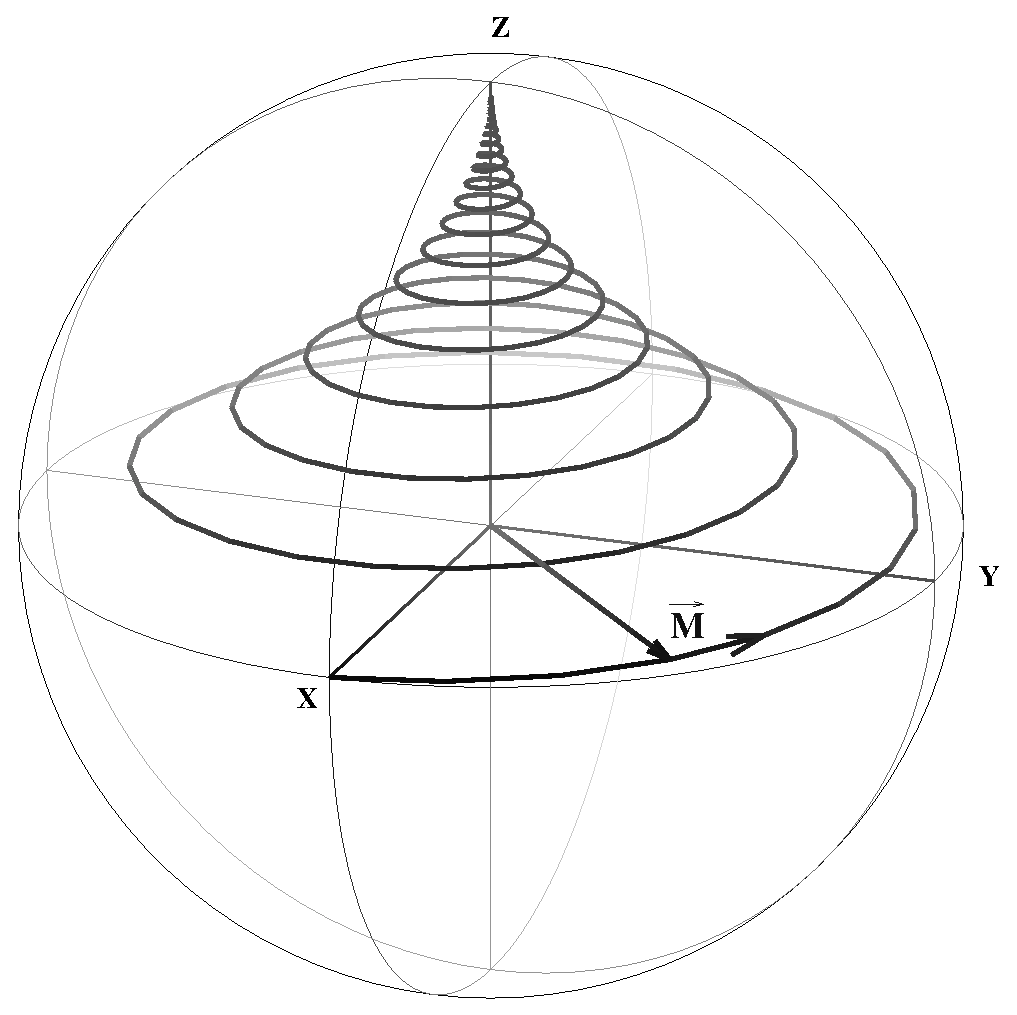
\epsfig{file=retour.eps,width=4in}
\end{center}
\caption{Retour à l'équilibre de l'aimantation macroscopique.}
\label{fig:retour}
\end{figure}

\section{Impulsions et onde continue}
Les noyaux de la même nature présents dans un échantillon n'ont généralement
pas tous la même fréquence de résonance, en particulier à cause de
l'effet différencié des électrons qui entourent les noyaux
(voir section \ref{sec:chemshift}).
Deux stratégies ont été successivement envisagées pour détecter et mesurer ces
différentes résonances et se traduisent par deux
façons différentes de manipuler le vecteur $\aimvec$ :
il s'agit des méthodes dites "par onde continue" et "par impulsion".
Cette dernière correspond à ce qui vient d'être présenté, à
savoir que $\aimvec$ est écarté de sa position initiale
et que $e(t)$ est analysée pendant la phase de retour à la situation initiale.
Sous réserve que la durée $T$ de la mise hors équilibre soit
suffisamment courte, et plus exactement que $1/T$ soit grand devant l'étendue de la
gamme de fréquences à considérer, tous les noyaux résonnant aux fréquences voisines
de celle de l'OEM subissent une perturbation identique.
La tension $e(t)$ recueillie aux bornes des spires au cours du retour
à la situation initiale est une somme de tensions
sinusoïdales de fréquences, d'amplitude et de phases différentes.
Le traitement de $e(t)$ nécessite des opérations de changement de fréquence
(toutes les fréquences sont diminuées d'une même quantité par un dispositif
électronique afin d'en faciliter le traitement ultérieur),
d'échantillonnage ($e(t)$ est mesurée à des intervalles de temps
réguliers) et de conversion analogique-digitale
(les résultats des mesures de $e(t)$ sont
converties en nombres binaires).
Il en résulte un ensemble de valeurs numériques,
manipulables par un calculateur,
qui contient toute l'information présente dans $e(t)$.
Pour un spectre de RMN du proton enregistré dans des conditions standard,
le temps nécessaire à l'acquisition des données est inférieur à 5 secondes.
L'analyse harmonique de $e(t)$ (sous forme numérique) est ensuite réalisée :
on obtient pour chaque fréquence l'intensité de la résonance.
Formellement, une fonction du temps $e(t)$ a été convertie en une fonction $S(\omega)$
appelée spectre.
Dans la pratique, le signal numérisé $S(\omega)$ se déduit de $e(t)$ par
transformation de Fourier, opération mathématique qui est calculée à l'aide
d'algorithmes rapides.

Pour des raisons technologiques, la recherche des
fréquences de résonance s'est d'abord effectuée
en faisant varier régulièrement et de façon
lente la fréquence $\nurf$ de l'OEM excitatrice.
L'absorption d'énergie est détectée par la mesure du
coefficient de surtension d'un circuit oscillant dont l'élément inductif est la bobine
d'excitation.
Une solution plus simple encore techniquement consiste à maintenir
constante la fréquence de l'OEM excitatrice et de faire varier régulièrement l'intensité
du champ magnétique $\bzeros$.
Pour obtenir un spectre de bonne qualité, il faut que $\bzeros$ ou $\nurf$ varie
lentement.
Typiquement, un spectre de proton standard était enregistré en 10 minutes
environ.

Le développement des techniques impulsionnelles se comprend aisément lorsque
l'on compare les possibilités d'amélioration du rapport signal/bruit des spectres.
Pendant les 10 minutes de l'enregistrement du spectre par la méthode de l'onde
continue, il est possible de répéter $N$ fois ($N = 100$, par exemple) le cycle
impulsion-acquisition et de co-additionner les valeurs de $e(t)$
(mises sous forme numérique) pour chaque valeur de $t$.
Une telle manipulation augmente dans un facteur $N$ le signal réellement
dû à la réponse des molécules et par un facteur $\sqrt{N}$ le bruit de fond crée par
les circuits électronique et dont la nature est aléatoire.
Le rapport Signal sur bruit (S/B) est amélioré dans un rapport $\sqrt{N}$
(soit 10 dans l'exemple choisi).
Il a été néanmoins possible d'améliorer aussi le rapport S/B
des spectre en onde continue en additionnant des spectres enregistrés successivement
dans les mêmes conditions.
L'obtention de spectres de \carb en abondance naturelle est
pratiquement irréalisable sans faire appel à l'accumulation rapide de spectres telle
qu'elle est effectuée par la méthode impulsionnelle.

L'élaboration d'expériences où les noyaux atomiques ne sont pas sollicités par
une seule impulsion mais par des trains (ou séquences) d'impulsions séparés par des
délais fixes ou variables, ouvre la voie à des méthodes d'investigation structurale
extrêmement puissantes.
Ces méthodes n'ont pas leur équivalent dans le domaine de
l'enregistrement en onde continue et s'appliquent aux molécules en solution, à l'état
solide et en imagerie médicale.

\section{Déplacement chimique, couplages}
\label{sec:chemshift}
Ce qui précède pourrait laisser penser que pour un type de noyau donné,
caractérisé par son rapport gyromagnétique la fréquence de résonance n'est déterminé
que par l'intensité $\bzeros$ du champ magnétique.
Si cela était réellement le cas la RMN serait restée une curiosité de
laboratoire, un peu comme si en spectroscopie infra-rouge toutes les fréquences de
vibration moléculaire correspondaient à un nombre d'onde de 3000 cm$^{-1}$.

Les électrons entourant un noyau créent un champ magnétique supplémentaire
sous l'influence du champ $\bzerovec$.
Il en résulte que le champ magnétique réellement perçu
par le noyau, $\bzerovecloc$, dépend de la densité électronique au
voisinage de ce noyau.
L'environnement chimique d'un noyau, c'est à dire la nature des atomes et des liaisons
environnantes est donc traduite par des valeurs particulières de
$\bzerolocs$.

$\bzerolocs$ est plus faible que $\bzeros$ et la différence est
proportionnelle à $\bzeros$.
Le facteur de proportionnalité est appelé constante d'écran (les électrons font écran
à $\bzerovec$ et noté $\sigma$ :
\begin{equation}
\bzerolocs = \bzeros(1-\sigma).
\end{equation}
La relation entre $\sigma$ et la fonction de densité électronique est connue
de manière théorique et les calculs correspondants sont réalisables en quelques minutes
pour des molécules peu complexes (quelques dizaines d'atomes) sur des ordinateurs
accessibles aux centres académiques.

Le coefficient $\sigma$ varie le plus souvent dans un intervalle restreint,
de 10$^{-5}$ pour les protons, de 2.10$^{-4}$ pour les noyaux de $^{13}$C.
La grandeur utilisée pratiquement n'est pas $\sigma$ mais le déplacement chimique
noté $\delta$, défini par rapport à la fréquence de
résonance d'un noyau d'une substance de référence comme le tétraméthylsilane
(TMS) pour les noyaux \prot et \carb.
La grandeur $\delta$ est sans unité :

\begin{equation}
\delta = \frac{\nu - \nutms}{\nutms}\times 10^6.
\end{equation}
L'usage a fait de $\delta$ une grandeur exprimée en ppm, ou parties par million.

L'existence d'un déplacement chimique bien défini présuppose que $\sigma$ ne dépend
pas de l'orientation relative de la molécule et de $\bzerovec$.
Ceci est faux en général, mais en phase liquide seule
une valeur moyenne de $\sigma$ est observée.
L'effet d'écran n'est décrit correctement qu'à
l'aide d'une matrice (ou tenseur) d'écran.

Le spectre de proton d'un composé organique en solution présente généralement
beaucoup plus de raies qu'il n'y a de type de protons chimiquement différents.
Cela est dû à une interaction magnétique entre noyaux appelée couplage scalaire
et dont le médiateur est le nuage électronique qui entoure les noyaux.
L'interaction magnétique directe à travers l'espace, appelée couplage
dipolaire, possède une moyenne nulle en milieu liquide isotrope mais est responsable
en partie des phénomènes de relaxation.
Dans les solides, le caractère tensoriel de l'effet d'écran et
le couplage dipolaire extrêmement intense (par comparaison
avec les couplages scalaires) donnent lieu à des spectres très complexes
qui peuvent être simplifiés par des techniques dédiées.

Les chapitres suivants seront essentiellement consacrés à la manipulation
de l'aimantation d'un échantillon sous l'influence de
$\bzerovec$, des couplages scalaires, ainsi que du
champ électromagnétique excitateur.
Ils constituent une base de connaissance nécessaire à la compréhension
des expériences usuelles utilisées pour l'analyse structurale
des molécules.


\chapter[RMN par TF]{Impulsions et transformation de Fourier}
\label{chap:bloch}

Le but de ce chapitre est de donner les bases théoriques de la
RMN impulsionnelle, technique qui a largement supplanté la
méthode du passage lent (dit par "onde continue")
grâce aux avantages qu'elle procure en termes de sensibilité
principalement.
Le nombre de pages consacrées à ce sujet ne présage pas de la
difficulté de la pratique de l'enregistrement de spectres par
transformation de Fourier.
L'enchaînement de toutes les opérations mentionnées,
de la génération des impulsions au tracé du spectre,
est totalement automatisable et transparent à l'utilisateur
dépourvu de curiosité.

\section{Équation simplifiée d'évolution de l'aimantation}
Le système que nous étudions est un ensemble de noyaux isolés les uns des
autres et tous magnétiquement équivalents.
Il peut par exemple s'agir des noyaux \prot d'un échantillon de
molécules de chloroforme CHCl$_3$ en solution dans du chloroforme deutéré,
en ne considérant que les molécules où l'atome de carbone est l'isotope
$^{12}$C (99 \% des cas) de spin nul.
Le cadre théorique de la description des phénomènes physiques
est celui de la mécanique classique, étant donné que
seule sera considérée l'évolution de l'aimantation macroscopique
de l'échantillon.
L'aimantation totale initiale de l'échantillon, notée $\aimzerovec$,
(définie au paragraphe \ref{sec:macro}) est soumise à
l'action du champ magnétique $\bzerovec$ seul avant toute
impulsion de l'OEM excitatrice, et après, pendant la
période de détection du signal.
Pendant l'impulsion, il faut tenir compte en plus de
l'action du champ de radio-fréquence.

Le champ magnétique $\bzerovec$ étant uniforme,
son action sur un système de moment magnétique $\aimvec$
se réduit à un couple de force $\Gammavec$ :
\begin{equation}
\Gammavec = \aimvec \wedge \bzerovec
\end{equation}
Ce couple de forces modifie le moment cinétique total
$\elvec$ des noyaux de l'échantillon
suivant le principe fondamental de la dynamique :
\begin{equation}
\derivt{\elvec} = \Gammavec = \aimvec \wedge \bzerovec
\end{equation}
Le moment magnétique total $\aimvec$ est le produit du moment
cinétique total $\elvec$ par le rapport
gyromagnétique des noyaux :
\begin{equation}
\aimvec = \gamma \elvec
\end{equation}
Ainsi
\begin{equation}
\label{eqn:bloch0}
\derivt{\aimvec} = \gamma \aimvec \wedge \bzerovec
\end{equation}
Les grandeurs $\gamma$ et $\bzerovec$ sont des données
constantes du problème.
L'équation \ref{eqn:bloch0} est l'équation du mouvement de
$\aimvec$, la résoudre c'est rechercher
l'expression de $\aimvect$ à partir d'un état initial défini en $t=0$.

Si à un instant donné, $\aimvec$ est l'aimantation d'équilibre
de l'échantillon $\aimzerovec$, et donc a la même
direction que $\bzerovec$,
alors $\derivttxt{\aimvec}$ est nulle et donc $\aimvec$ reste constant.
Il n'y a dans ce cas pas d'évolution de $\aimvec$, ce qui est
le propre d'un état d'équilibre.
Dans le paragraphe qui suit, on considère que $\aimvec$
a déjà été mise hors équilibre au moyen d'une impulsion de
radiofréquence.
On considère d'autre part que seule l'action de $\bzerovec$
s'exerce sur $\aimvec$,
les phénomènes de relaxation n'étant pas pris en compte.

\section{La précession de Larmor}
\label{sec:larmor}
Si $\kvec$ est le vecteur unitaire ayant le sens
et la direction de $\bzerovec$,
\begin{equation}
\bzerovec = \bzero \kvec
\end{equation}
et donc
\begin{equation}
\derivt{\aimvec} = \gamma \bzero \aimvec \wedge \kvec
\end{equation}
Si on pose
\begin{equation}
\gamma \bzeros = -\omega_0,
\end{equation}
l'équation qui régit les variations de l'aimantation totale des
noyaux considérés est :
\begin{equation}
\label{eqn:bloch1}
\derivt{\aimvec} = \omega_0 \kvec \wedge \aimvec
\end{equation}
Sans résoudre cette équation différentielle il est possible d'en déduire quelques
propriétés de l'évolution de $\aimvec$
lorsque $\bzerovec$ est constant.
L'égalité obtenue en prenant le produit scalaire des deux membres de
l'équation \ref{eqn:bloch1} par $\kvec$\ s'écrit
\begin{equation}
\derivt{(\kvec.\aimvec)} = \omega_0 (\kvec \wedge \aimvec).\kvec = 0
\end{equation}
car le produit vectoriel $\kvec \wedge \aimvec$
est perpendiculaire à $\kvec$
(et à $\aimvec$).
La grandeur $\kvec.\aimvec$ est la
mesure algébrique $\aimzs$ de la projection $\aimzvec$
de $\aimvec$ sur l'axe de $\kvec$ (axe $Oz$, figure \ref{fig:mxyz}).
La quantité $\aimzs$ est donc invariable au cours du temps.

Le produit scalaire des deux membres de l'équation \ref{eqn:bloch1}
par $\aimvec$ donne :
\begin{equation}
\label{eqn:normcnste}
\derivt{\aimvec}.\aimvec = 
\omega_0 (\kvec \wedge \aimvec).\aimvec = 0
= \frac{1}{2}.\derivt{\aims^2}
\end{equation}
La norme $\aims$ du vecteur $\aimvec$ est donc invariante au cours du temps.
Si $\theta$ est l'angle entre les directions des vecteurs
$\aimvec$ et $\kvec$,
alors $\aimzs = \aims\cos\theta$.
Sachant que $\aimzs$ et $\aims$ sont constants,
$\aimvec$ évolue en
faisant un angle constant avec $\bzerovec$.

\begin{figure}[hbt]
\begin{center}
\begin{pspicture}(-3,-1)(4,5)
\SpecialCoor
\uput{10pt}[-165](0,0){$O$}
\psline{->}(1;170)(5;-10)
\uput[-90](5;-10){$x$}
\psline{->}(0,0)(1;-10)
\uput[-90](1;-10){$\ivec$}
\psline{->}(1;-140)(5;40)
\uput[40](5;40){$y$}
\psline{->}(0,0)(1;40)
\uput{4pt}[-20](1;40){$\jvec$}
\psline{->}(1;-90)(5;90)
\uput[180](5;90){$z$}
\psline{->}(0,0)(1;90)
\uput[180](1;90){$\kvec$}
\psset{linewidth=0.08}
\psline{->}(0,0)(2,0.5)
\uput[0](2,0.5){$\aimxyvec$}
\psline{->}(0,0)(2,3.5)
\uput[60](2,3.5){$\aimvec$}
\psline{->}(0,0)(0,3)
\uput[135](0,3){$\aimzvec$}
\psline[linestyle=dashed,dash=3pt 3pt](2,0.5)(2,3.5)
\psline[linestyle=dashed,dash=3pt 3pt](0,3)(2,3.5)
\psline{->}(-2,-0.5)(-2,1.5)
\uput{3pt}[45](-2,1.5){$\bzerovec$}
\psset{linewidth=0.02}
\psellipse(0,3)(!4 3 sqrt div 1)
\pscurve{->}(0,1.5)
(!1 1 1 mul 3.5 3.5 mul add sqrt div 1.4 mul 3.5 1 1 mul 3.5 3.5 mul add sqrt div 1.4 mul)
(!2 2 2 mul 3.5 3.5 mul add sqrt div 1.3 mul 3.5 2 2 mul 3.5 3.5 mul add sqrt div 1.3 mul)
\rput(0.4,1.6){$\theta$}
\end{pspicture}
\caption{\label{fig:mxyz}
\small Décomposition de l'aimantation en composantes transversale et longitudinale.}
\end{center}
\end{figure}

Si on décompose $\aimvec$ en la somme des deux vecteurs
$\aimzvec$ et $\aimxyvec$ comme indiqué sur la figure \ref{fig:mxyz},
l'équation \ref{eqn:bloch1} devient
\begin{equation}
\derivt{(\aimxyvec+\aimzvec)} = \omega_0 \kvec \wedge (\aimxyvec+\aimzvec)
\end{equation}
Or $\derivttxt{\aimzvec}$ = 0 et
$\kvec \wedge \aimzvec$ = 0
(ces deux vecteurs sont colinéaires).
L'équation qui régit les variations de $\aimxyvec$
est donc formellement la même que celle qui régit celles de
$\aimvec$ :
\begin{equation}
\label{eqn:blochxy}
\derivt{\aimxyvec} = \omega_0 \kvec \wedge \aimxyvec
\end{equation}

Le vecteur $\aimxyvec$ est la projection de
$\aimvec$ dans le plan perpendiculaire à la direction de
$\bzerovec$.
Sa norme est constante (équation \ref{eqn:normcnste}
appliquée à $\aimxyvec$).
La norme de la variation de $\aimxyvec$
est constante (équation \ref{eqn:blochxy}) puisque
$\aimxyvec$ et $\kvec$ sont des vecteurs
de norme constante et qu'il sont en permanence orthogonaux.
Le vecteur $\derivttxt{\aimxyvec}$ est perpendiculaire en
permanence à $\aimxyvec$.
Le mouvement de $\aimxyvec$ qui répond à tous ces critères
ne peut être qu'un mouvement circulaire uniforme.
L'extrémité du vecteur $\aimvec$ décrit donc
un mouvement de rotation uniforme autour de $\kvec$,
c'est-à-dire au tour de $\bzerovec$,
en faisant avec ce dernier un angle constant $\theta$.

La résolution explicite de l'équation \ref{eqn:blochxy} permettra de préciser la
fréquence et le sens de la rotation de $\aimvec$
autour de $\bzerovec$.
Les vecteurs figurant dans l'équation différentielle \ref{eqn:blochxy}
seront projetés sur deux axes $Ox$ et $Oy$
portant les vecteurs unitaires $\ivec$,
$\jvec$, tous deux orthogonaux à $\kvec$
et qui définissant ce qui est communément appelé le plan transversal $xOy$.

En posant
\begin{equation}
\aimxyvec = \aimxs \ivec + \aimys \jvec
\end{equation}
l'équation \ref{eqn:blochxy} devient
\begin{equation}
\derivt{\aimxs} \ivec + \derivt{\aimys} \jvec =
\omega_0 (\kvec \wedge \ivec)\aimxs +
\omega_0 (\kvec \wedge \jvec)\aimys =
\omega_0 \aimxs \jvec -
\omega_0 \aimys \ivec
\end{equation}
et donc
\begin{eqnarray}
\label{eqn:mx}
\derivt{\aimxs} & = & -\omega_0 \aimys \\
\label{eqn:my}
\derivt{\aimys} & = & +\omega_0 \aimxs
\end{eqnarray}

En dérivant par rapport au temps les deux membres de l'équation \ref{eqn:mx},
et en remplaçant $\derivttxt{\aimys}$ par son expression issue de
l'équation \ref{eqn:my} on obtient :
\begin{equation}
\dderivt{\aimxs} = -\omega_0^2 \aimxs
\end{equation}
Les solutions de cette équation sont de la forme
\begin{equation}
\label{eqn:mxlarmor}
\aimxs = A\cos(\omega_0 t + \phi)
\end{equation}
où $A$ et $\phi$ sont des constantes déterminées par les valeurs initiales de
$\aimxs$ et $\aimys$.
$\aimys$ se déduit de l'équation \ref{eqn:mx} :
\begin{equation}
\label{eqn:mylarmor}
\aimys = A\sin(\omega_0 t + \phi)
\end{equation}
La constante $A$ est déterminée sachant que
\begin{equation}
A^2 = \aimxs^2 + \aimys^2
\end{equation}
et donc que $A$ est la norme du vecteur $\aimxyvec(t=0)$,
vecteur $\aimxyvec$ pris à l'instant où
l'évolution libre de l'aimantation commence.
A cet instant $\aimxs$ et $\aimys$ valent
$\aimxys(t=0).\cos\phi$ et
$\aimxys(t=0).\sin\phi$.
L'angle $\phi$ est celui que fait
$\aimxyvec(t=0)$ avec l'axe $Ox$ à l'instant $t = 0$.

La quantité $\omega_0$, appelée pulsation propre, définit la fréquence propre
$\nu_0$ de rotation de l'aimantation autour de l'axe $Oz$ :
\begin{equation}
\nu_0 = \omega_0 / 2\pi
\end{equation}

Lorsque l'échantillon est plongé dans le champ magnétique
$\bzerovec$ il acquiert un moment
magnétique $\aimzerovec$ aligné avec $\bzerovec$ ;
$\aimxyvec(t=0)$ est donc nul et reste nul aussi longtemps que
$\aimvec$ n'interagit qu'avec $\bzerovec$.
Ce n'est que lorsqu'une impulsion de radio-fréquence aura écarté
$\aimvec$ de sa position initiale que son mouvement sera la rotation qui vient
d'être déterminée (Figure \ref{fig:larmor}).
Ce mouvement est appelé précession de Larmor et s'effectue à la fréquence
\begin{equation}
 \fbox{$ \displaystyle
\nu_0 = -\frac{\gamma \bzeros}{2\pi}
 $}
\end{equation}

\begin{figure}[hbt]
\begin{center}
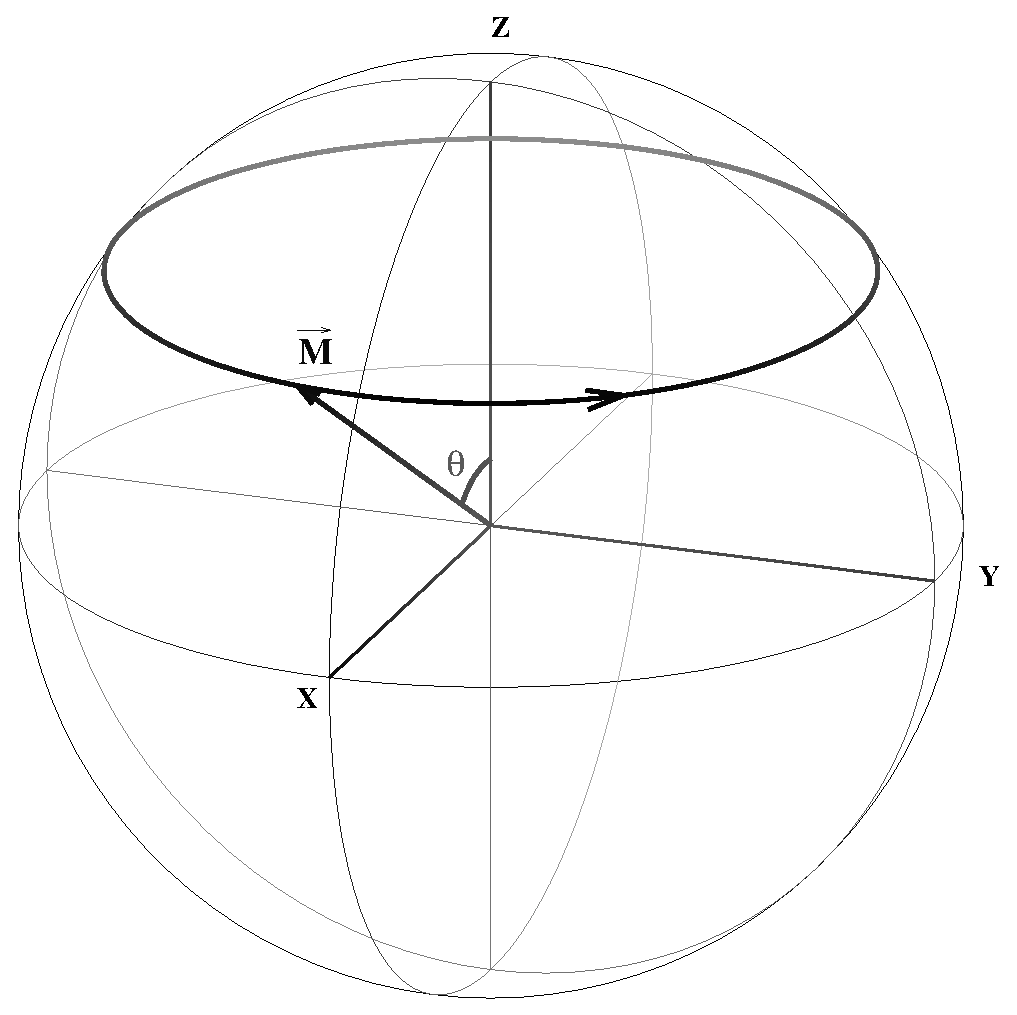
\epsfig{file=larmor.eps,width=4in}
\end{center}
\caption{Précession de Larmor.}
\label{fig:larmor}
\end{figure}

\section{Impulsion, référentiel tournant}
\label{sec:rf}
Le processus qui conduit de l'état d'équilibre $\aimzerovec$ de $\aimvec$
à un état excité résulte de l'action
d'un champ magnétique créé par un courant alternatif sinusoïdal de radiofréquence,
supposé aligné avec l'axe $Ox$ et égal à
\begin{equation}
\bunvect =
2\bunmax \cos(\omrf t+\phi) \ivec
\end{equation}

La pulsation $\omrf$ du champ variable $\bunvect$
est a priori quelconque.
L'angle $\phi$ est appelé la phase de l'impulsion.

De fait, et par la vertu des équations de Maxwell, le champ variable
$\bunvect$ est associé à un champ électrique variable.
L'association de ces deux champs constitue ce qui jusqu'à présent
était désigné sous le terme un peu vague d'OEM excitatrice.
Le fait est que seule la composante magnétique de cette onde
interagit avec les spins nucléaires.
L'interaction de l'OEM avec le système étudié peut donc légitimement
être étudiée comme étant restreinte à la seule action de la composante magnétique
de l'onde excitatrice.
Le champ de radiofréquence est créé par les bobines (dont la géométrie
réelle peut être très éloignée de l'idée de ce que l'on peut se faire d'une bobine,
voir figure \ref{fig:coil})
qui entourent l'échantillon et qui servent à la fois à recueillir les variations
de l'aimantation de l'échantillon sous forme de force électromotrice induite,
mais aussi à exciter l'échantillon lorsqu'elles sont parcourues par
un courant alternatif sinusoïdal de fréquence $\omrf/2\pi$.

\begin{figure}[hbt]
\begin{center}
\begin{pspicture}(-2.5,-2)(2.5,4.5)
\SpecialCoor
\psline(-0.5,4)(-0.5,-1.5)
\psarc(0,-1.5){0.5}{180}{0}
\psline(0.5,4)(0.5,-1.5)
\psellipse(0,1.5)(0.5,0.25)
\psellipse(0,4)(0.5,0.25)
\psline(-2.5,0)(2.5,0)
\psline(0,0.1)(0,-0.1)
\uput[135](0,0){$O$}
\psset{linewidth=0.05}
\psline(-2.5,-1)(-1.5,-1)
\psline{->}(-2.5,-1)(-1.5,-1)
\rput(-1,0){
\pscurve(-0.5,-1)(-0.3,-1)(0,-0.9)(0.2,0)(0,1)(-0.2,0)(0,-0.9)(0.3,-1)(0.5,-1)
}
\psline(-0.5,-1)(0.5,-1)
\rput(1,0){
\pscurve(-0.5,-1)(-0.3,-1)(0,-0.9)(0.2,0)(0,1)(-0.2,0)(0,-0.9)(0.3,-1)(0.5,-1)
}
\psline(1.5,-1)(2.5,-1)
\psline{->}(0,0)(2,0)
\uput[90](2,0){$\bunvect$}
\uput[-90](-1.5,-1){$\boldsymbol{I(t)}$}
\psline{->}(0,0)(0,3)
\uput[90](0,3){$\bzerovec$}
\end{pspicture}
\caption{\label{fig:coil}
% \small Création du champ excitateur $\bunvect$.}
\small Création du champ excitateur.}
\end{center}
\end{figure}

Il est commode de considérer $\bunvect$ comme la
superposition de deux champs magnétiques tournants
$\bunvecplus$ et $\bunvecmoins$ tels que :
\begin{eqnarray}
\bunvecplus & = &
\bunmax\cos(\omrf t + \phi) \ivec +
\bunmax\sin(\omrf t + \phi) \jvec \\
\bunvecmoins & = &
\bunmax\cos(\omrf t + \phi) \ivec -
\bunmax\sin(\omrf t + \phi) \jvec
\end{eqnarray}

Cette décomposition est la même que celle introduite lorsqu'il est dit
que la lumière polarisée linéairement peut être considérée comme
la superposition de lumières polarisées circulairement à droite
et à gauche.

Les vecteurs $\bunvecplus$ et $\bunvecmoins$
tournent respectivement dans le plan $xOy$ aux pulsations $+\omrf$ et
$-\omrf$.
Il suffit d'analyser l'action d'un seul de ces deux champs,
$\bunvecplus$ par exemple,
car un seul des deux exerce une influence sur l'aimantation
$\aimvec$ (voir ci-dessous).
Pour la commodité nous écrirons :
\begin{equation}
\label{eqn:bunvect}
\bunvect =
(\bunmax\cos(\omrf t + \phi)\ivec + \bunmax\sin(\omrf t + \phi)\jvec)
\end{equation}

L'équation \ref{eqn:bloch0} devient
\begin{equation}
\label{eqn:blochrf0}
\derivt{\aimvec} = \gamma \aimvec \wedge (\bzerovec + \bunvect)
\end{equation}

Si on définit
\begin{equation}
\omuns = -\gamma \bunmax
\end{equation}

l'équation \ref{eqn:blochrf0} devient
\begin{equation}
\label{eqn:blochrf1}
\derivt{\aimvec} =
(\omega_0 \kvec + \omuns(\cos(\omrf t + \phi) \ivec + \sin(\omrf t + \phi) \jvec))
\wedge \aimvec
\end{equation}

La résolution de cette équation où le champ magnétique dépend du temps
est facilitée si on change les axes de projection $Ox$, $Oy$
et $Oz$ de façon à rendre le second membre de l'équation \ref{eqn:blochrf1} indépendant
du temps.
Cela est réalisé en choisissant d'observer $\aimvec$ dans un repère tournant
autour de l'axe $Oz$ à la
pulsation $\omrf$ de la composante du champ magnétique excitateur
qui tourne dans le même sens que $\aimvec$ (figure \ref{fig:refer}).
Dans ce repère d'observation, le champ magnétique $\bunvect$
(ou plus exactement la composante tournante retenue) paraîtra immobile.
Le repère (ou référentiel) tournant aura pour axes $OX$, $OY$ et $OZ$,
portant respectivement les vecteurs unitaires
$\iprimvec$, $\jprimvec$ et $\kprimvec$.
Ces vecteurs sont choisis de façon à coïncider avec
$\ivec$, $\jvec$ et $\kvec$
à l'instant $t$ = 0 de l'établissement du champ $\bunvect$.
Les axes $Oz$ et $OZ$ restant en permanence confondus,
on a : $\kvec = \kprimvec$.

\begin{figure}[hbt]
\begin{center}
\begin{pspicture}(-4,-1)(4,4)
\SpecialCoor
\psline{->}(-4,0)(4,0)
\uput[-90](4,0){$x$}
\psline{->}(0,-1)(0,4)
\uput[180](0,4){$y$}
\uput{7pt}[-120](0,0){$O$}
\psline{->}(0.5;-150)(4;30)
\uput[30](4;30){$X$}
\psline{->}(0.5;-60)(4;120)
\uput[120](4;120){$Y$}
\pscircle*(-3,1){0.02}
\pscircle(-3,1){0.2}
\psset{linewidth=1.2pt}
\psline{->}(0,0)(2;0)
\uput[-90](2;0){$\ivec$}
\psline{->}(0,0)(2;90)
\uput[180](2;90){$\jvec$}
\psline{->}(0,0)(2;30)
\uput[120](2;30){$\iprimvec$}
\psline{->}(0,0)(2;30)
\uput[-150](2;120){$\jprimvec$}
\uput{8pt}[90](-3,1){$\kvec=\kprimvec$}
\psset{linewidth=0.08pt}
\psarc[arcsepB=1.2pt]{->}(0,0){2.5}{0}{30}
\uput[15](2.5;15){$\omrft$}
\end{pspicture}
\caption{\label{fig:refer}
\small Référentiel du laboratoire et référentiel tournant.}
\end{center}
\end{figure}

Ce changement de repère apporte le résultat souhaité (annexe \ref{chap:refer} pour le détail des
calculs), à savoir de faire disparaître les termes dépendants du temps.
L'équation \ref{eqn:blochrf1} devient identique dans sa forme à l'équation
\ref{eqn:bloch1}.
\begin{equation}
\label{eqn:blochrf2}
\derivt{\aimvec} = \omveceff \wedge \aimvec
\end{equation}

L'axe et la pulsation de la précession de Larmor dans le référentiel tournant sont donnés
par la direction et la mesure algébrique de $\omveceff$ (figure \ref{fig:effectif}) :
\begin{equation}
\omveceff =
(\omega_0 - \omrf) \kvec + \omuns \uvec = \omzerovec + \omunvec
\end{equation}
où le vecteur unitaire $\uvec$ est fixe dans le repère tournant
et reflète la phase de l'impulsion :
\begin{equation}
\uvec =
\cos\phi\iprimvec +
\sin\phi\jprimvec
\end{equation}

\begin{figure}[hbt]
\begin{center}
\begin{pspicture}(-1,-1)(4,5)
\SpecialCoor
\uput{10pt}[-165](0,0){$O$}
\psline{->}(1;170)(5;-10)
\uput[0](5;-10){$X$}
\psline{->}(0,0)(1.5;-10)
\uput[-90](1.5;-10){$\iprimvec$}
\psline{->}(1;-140)(5;40)
\uput[40](5;40){$Y$}
\psline{->}(0,0)(1.5;40)
\uput{4pt}[-20](1.5;40){$\jprimvec$}
\psline{->}(1;-90)(5;90)
\uput[180](5;90){$Z$}
\psline{->}(0,0)(1.5;90)
\uput[180](1.5;90){$\kprimvec$}
\psset{linewidth=1.2pt}
\psline{->}(0,0)(2,0.5)
\uput[0](2,0.5){$\omunvec$}
\psline{->}(0,0)(!1.5 2 mul 2 2 mul 0.5 0.5 mul add sqrt div 1.5 0.5 mul 2 2 mul 0.5 0.5 mul add sqrt div)
\uput[-120](!1.5 2 mul 2 2 mul 0.5 0.5 mul add sqrt div 1.5 0.5 mul 2 2 mul 0.5 0.5 mul add sqrt div){$\uvec$}
\psline{->}(0,0)(2,3.5)
\uput[60](2,3.5){$\omveceff=-\gamma \bveceff$}
\psline{->}(0,0)(0,3)
\uput[135](0,3){$\omzerovec$}
\psline[linestyle=dashed,dash=3pt 3pt](2,0.5)(2,3.5)
\psline[linestyle=dashed,dash=3pt 3pt](0,3)(2,3.5)
\psset{linewidth=0.8pt}
\psarc{->}(0,0){1.75}{-10}{14.03}
\uput[2](1.75;2){$\phi$}
\end{pspicture}
\caption{\label{fig:effectif}
\small Action d'une impulsion de RF, vue dans le référentiel tournant.}
\end{center}
\end{figure}

Le champ de radiofréquence créé par les bobines excitatrices est donc
capable de faire tourner l'aimantation macroscopique autour d'un axe
lié au référentiel tournant.
La précession de Larmor dans le référentiel tournant est
amène l'aimantation de l'échantillon
hors de sa position d'équilibre.
Ce paragraphe offre une description beaucoup plus détaillée de ce qui est communément
traduit par la formule "l'aimantation s'est écartée de sa position d'équilibre car
l'échantillon a absorbé l'énergie fournie par le champ excitateur".

\section{Impulsion en résonance et hors résonance}
Dans ce paragraphe l'évolution de $\aimvec$ dans le référentiel tournant est analysé dans
différents cas de figure :
\begin{itemize}
\item $\bunvec$ est appliqué en résonance, c'est-à-dire que la fréquence de l'excitation
est exactement égale à la fréquence de résonance des noyaux considérés :
$\omrf = \omega_0$,
\item $\bunvec$ est "légèrement" hors résonance,
\item $\bunvec$ est "complètement" hors résonance.
\end{itemize}

Si la fréquence du champ $\bunvec$ est exactement égale à la fréquence de résonance des
noyau alors $\omveceff = \omunvec$.
Dès que $\bun$ n'est plus nul, $\aimvec$ tourne autour de
l'axe horizontal porté par le vecteur $\uvec$ à la fréquence $\omuns/2\pi$.
Si l'angle de phase $\phi$ est nul, l'axe de rotation de $\aimvec$ est l'axe $OX$
(Figure \ref{fig:onres}).

\begin{figure}[hbt]
\begin{center}
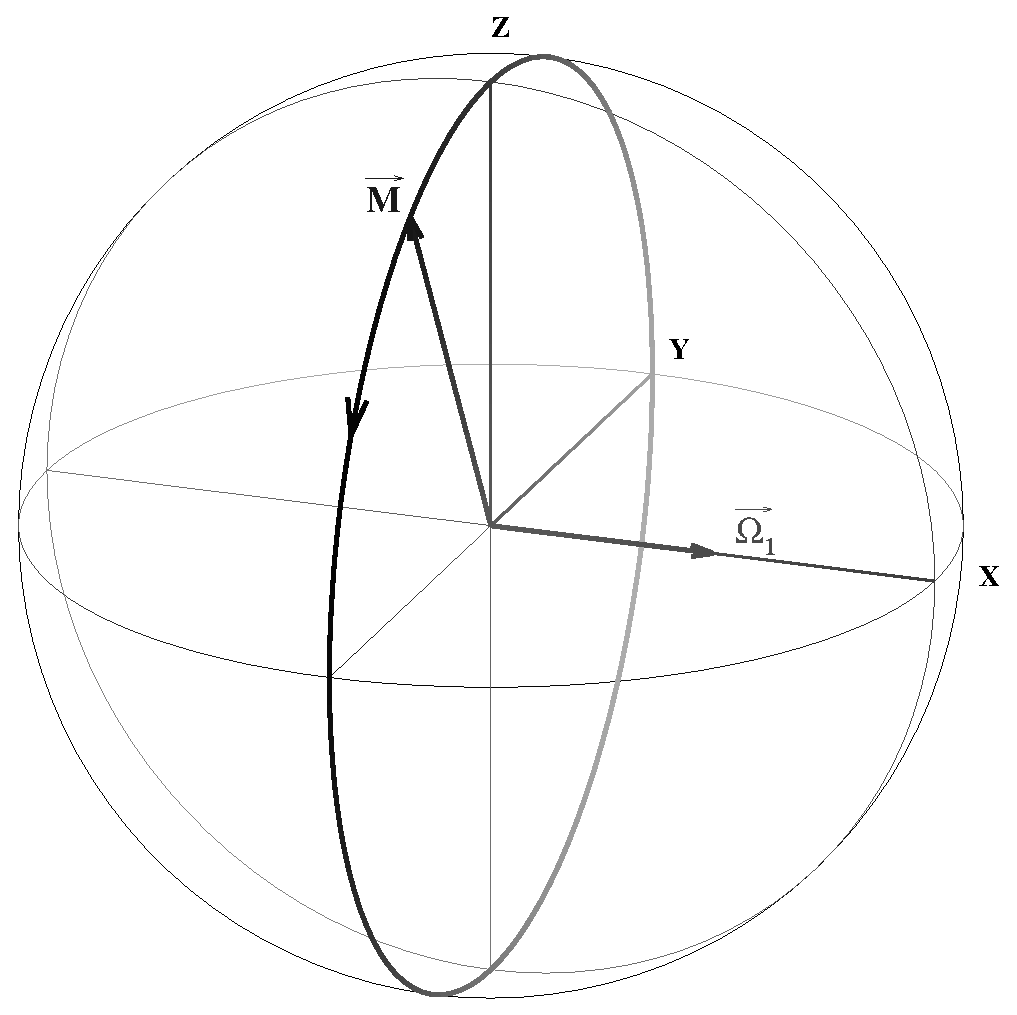
\epsfig{file=off0.eps,width=4in}
\end{center}
\caption{Excitation en résonance.}
\label{fig:onres}
\end{figure}

L'angle $\theta$ de la rotation de $\aimvec$ causée par l'application du champ $\bunvec$
pendant une durée $T$ vaut $\omuns T$.
Cet angle est aussi appelé angle de nutation.
S'il est égal à $\pi/2$, l'aimantation initialement dirigée selon l'axe $OZ$
devient $-\aimzeros\jprimvec$.
Le signe des angles de rotation résulte d'un certain nombre de conventions et
nous adopterons celle qui consiste à utiliser la règle du tire-bouchon :
Le tire-bouchon étant placé sur l'axe $OX$, il faut amener $\aimvec$ en direction
de l'axe $OY$ dans le sens des $Y$ négatifs pour faire avancer la vrille vers les $X$
positifs si l'angle $\theta$ est positif.

Pratiquement, les valeurs de la phase les plus utilisées sur un spectromètre
sont 0, $\pi/2$, $\pi$, $3\pi/2$.
Les impulsions correspondantes seront notées successivement $\theta_x$,
$\theta_y$, $\theta_{-x}$, $\theta_{-y}$ pour en rappeler
à la fois l'angle et l'axe de rotation.
L'effet de ces impulsions est donnée par le tableau \ref{tab:phase}.

\begin{table}
\caption{Action d'une impulsion de RF sur l'aimantation d'équilibre}
\label{tab:phase}
\begin{center}
\begin{tabular}[hbt]{ccc}
\hline
Impulsion & Phase($\phi$) & $\aimvec$ final \\ \hline
$\theta_{x}$  & $0$      & $-\aimzeros\sin\theta\jprimvec + \aimzeros\cos\theta\kprimvec$ \\
$\theta_{y}$  & $\pi/2$  & $+\aimzeros\sin\theta\iprimvec + \aimzeros\cos\theta\kprimvec$ \\
$\theta_{-x}$ & $\pi$    & $+\aimzeros\sin\theta\jprimvec + \aimzeros\cos\theta\kprimvec$ \\
$\theta_{-y}$ & $-\pi/2$ & $-\aimzeros\sin\theta\iprimvec + \aimzeros\cos\theta\kprimvec$ \\
\hline
\end{tabular}
\end{center}
\end{table}
Le vecteur $\aimvec$ à la fin de l'impulsion se réécrit de façon plus générale sous la forme :
\begin{equation}
\label{eqn:pulseaction}
\aimvec = \aimzeros \sin\theta (\cos(\phi-\pi/2)\iprimvec +
\sin(\phi-\pi/2)\jprimvec) + \aimzeros\cos\theta\kprimvec
\end{equation}
L'angle que fait la composante horizontale de $\aimvec$ avec le vecteur $\iprimvec$
est égal à la phase de l'impulsion, à $\pi/2$ près.

Des noyaux hors résonance sont caractérisés par leur "décalage" (offset)
à savoir la pulsation $\omzeros = \omega_0 - \omrf$.
Ils subissent en première approximation les mêmes actions dues au
champ $\bunvec$ si la condition $|\omzeros| << \omuns$ est vérifiée.
Cela nécessite un champ magnétique $\bunvec$ suffisamment intense pour
que $\omuns/2\pi$ soit grand par rapport à l'écart
entre la fréquence de résonance des noyaux et la fréquence des impulsions.
Plus $\bunvec$ sera intense et plus l'excitation des différents noyaux (de même nature)
de l'échantillon sera uniforme.
En conséquence les impulsions doivent être les plus courtes possible pour un
angle de rotation donné.
La durée des impulsions est généralement inférieure à 10 $\mu$s
pour un angle de $\pi/2$.

\begin{figure}[hbt]
\begin{center}
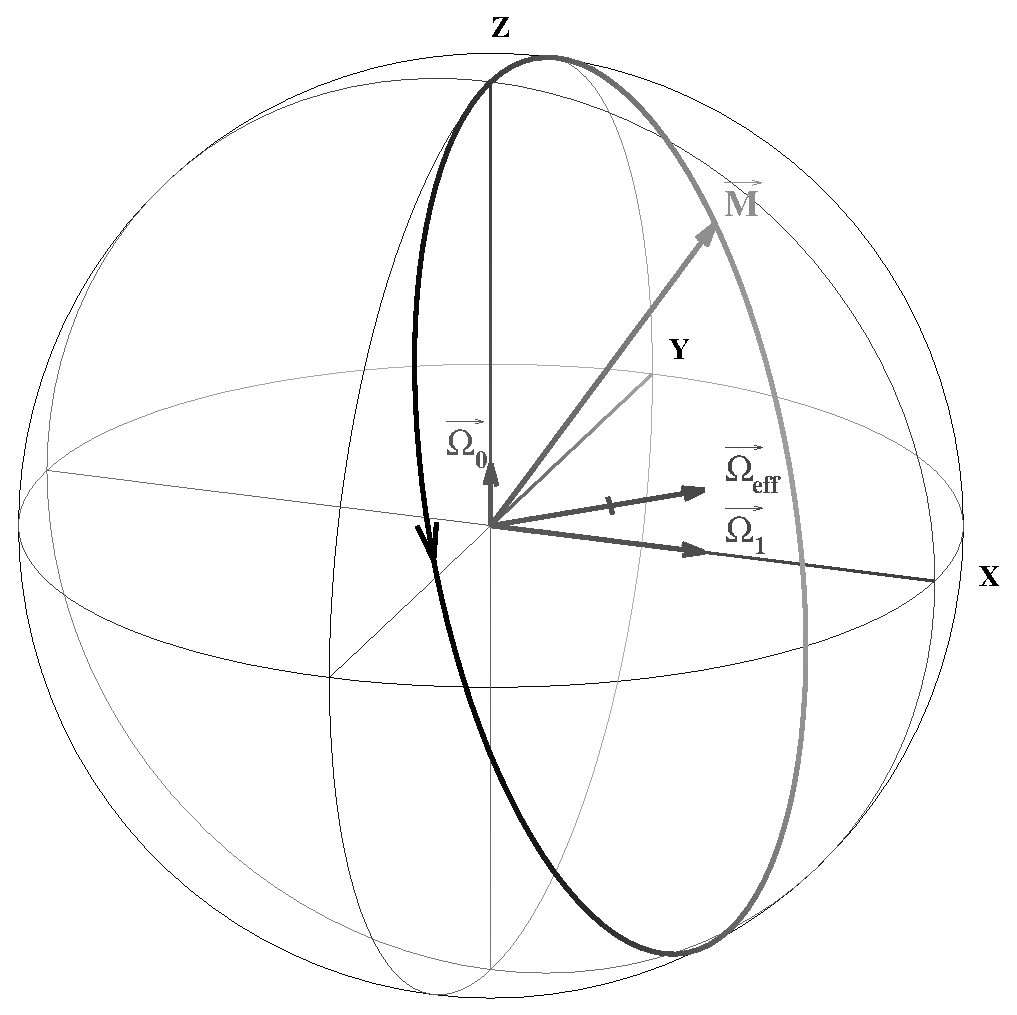
\epsfig{file=off1.eps,width=4in}
\end{center}
\caption{Excitation légèrement hors résonance.}
\label{fig:offres}
\end{figure}

Si $|\omzeros|$
 est de l'ordre de grandeur de $\omuns$
l'axe de rotation fait un angle $\theta$ significatif avec le plan
$XOY$ (Figure \ref{fig:offres}) :
\begin{equation}
\tan \theta =  \frac{\omzeros}{\omuns}
\end{equation}

La pulsation de rotation est la norme du vecteur $\omveceff$ :
\begin{equation}
\omeff = \sqrt{\omzeros^2 + \omuns^2}
\end{equation}
Dans le cas général la rotation de $\aimvec$ à partir de sa position d'équilibre
ne se fait plus exclusivement dans un plan vertical.

Si $\omuns$ est faible devant $\omzeros$,
les noyaux ne subissent pratiquement pas l'influence du champ de
radiofréquence, car ce dernier est appliqué très loin de la résonance
(Figure \ref{fig:veryoffres}).

Les noyaux de nature différente ont des gammes de fréquence de résonance
suffisamment éloignées les unes des autres pour que, par exemple, il soit impossible
d'exciter simultanément les protons et les noyaux de $^{13}$C avec une seule
impulsion.
Nous avons souligné qu'un champ magnétique linéaire $\bunvec$ de pulsation $\omrf$
résulte de la superposition de deux champs tournants de pulsation $+\omrf$ et $-\omrf$.
Dans les conditions usuelles où $\omega_0$ et $\omrf$ sont très proches,
$+\omrf$ et $-\omrf$ sont nécessairement très
éloignées.
Cela justifie le fait qu'une seule composante
circulaire de $\bunvec$ soit prise en compte dans les calculs.

\begin{figure}[hbt]
\begin{center}
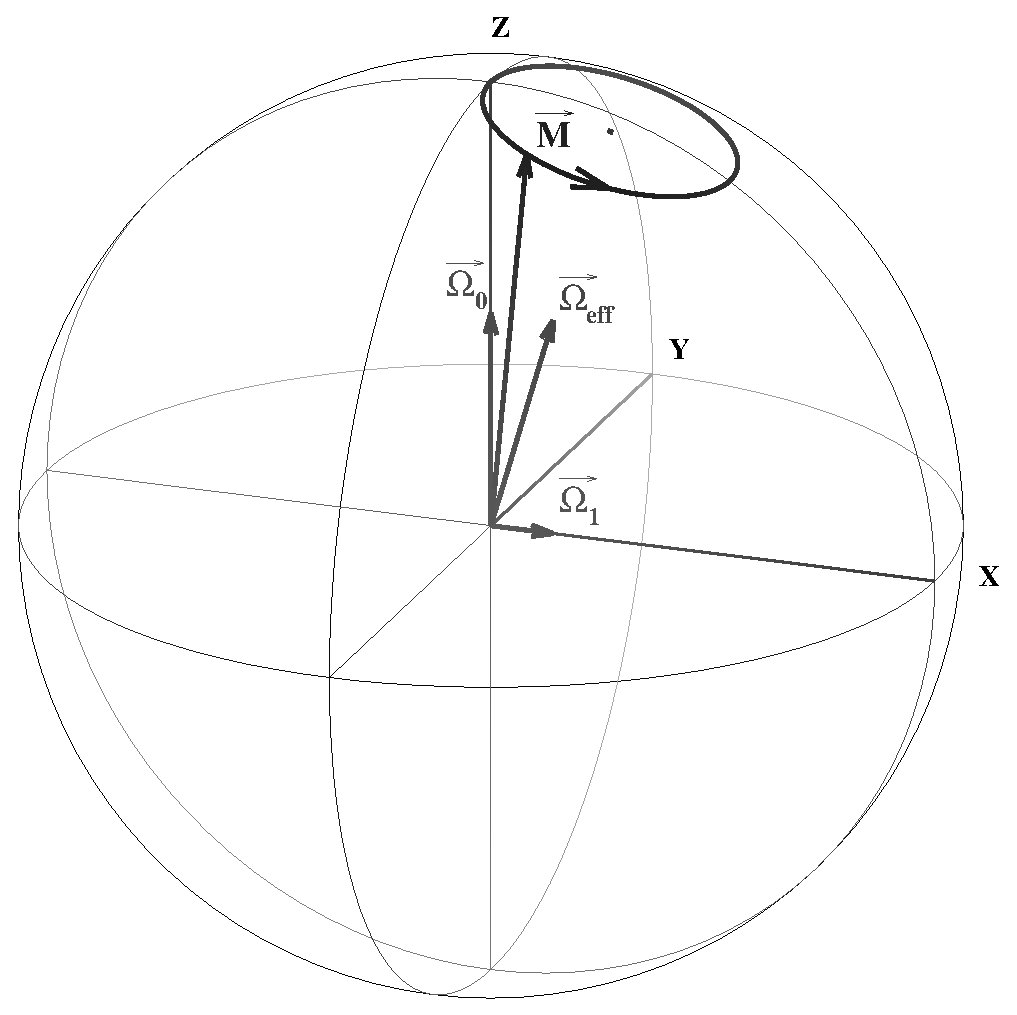
\epsfig{file=off2.eps,width=4in}
\end{center}
\caption{Excitation très loin de la résonance.}
\label{fig:veryoffres}
\end{figure}

\section{Après l'impulsion}
Lorsque $\bunvec$ redevient nul, le vecteur $\aimvec$ ne subit plus que l'action de
$\bzerovec$, et son mouvement dans le référentiel du laboratoire est le mouvement
de précession de Larmor de pulsation $\omega_0$ décrit au paragraphe \ref{sec:larmor}.

Sachant que le sens de rotation du référentiel tournant est celui de la
rotation libre (de Larmor) de $\aimvec$,
ce dernier tourne par rapport au référentiel tournant à la pulsation $\omzeros$
\begin{equation}
\omzeros = \omega_0 - \omrf
\end{equation}
sachant que le référentiel tournant tourne autour du référentiel du laboratoire
à la pulsation $\omrf$.

On constate que la description du mouvement de l'aimantation
macroscopique se résume (hors relaxation) à de simples rotations
si elle est effectuée dans le référentiel tournant.
Cette simplicité est liée au fait que dans ce référentiel tout
se passe comme $\aimvec$ n'était soumis qu'à des champs magnétiques constants.

\section{Relaxation}
Le traitement mécanique de l'évolution de l'aimantation d'un ensemble de noyaux tel
qu'il vient d'être traité néglige complètement l'effet de la relaxation, c'est à dire de
l'ensemble des phénomènes qui tendent à ramener $\aimvec$ à sa position initiale dès qu'elle
s'en écarte.
Il est commode pour étudier leur effet de se placer dans le référentiel
tournant à pulsation $\omzeros$, référentiel où $\aimvec$ paraît immobile en
l'absence de champ magnétique $\bunvec$ et de phénomènes de relaxation.
Sauf si les noyaux étudiés sont en résonance, il ne s'agit pas du référentiel tournant
au sens où il a été défini au paragraphe précédent.
Dans le référentiel d'étude, $\aimvec$ évolue en restant dans le plan $\Pi$ défini par $\aimvec$
et $\bzerovec$.

A chaque instant $t$ la variation des composantes $\aimzs$ et $\aimxys$ est proportionnelle à l'écart
entre leur valeur au temps $t$ et leur valeur d'équilibre :
\begin{eqnarray}
\label{eqn:t1}
\derivt{\aimzs} & = & -\frac{\aimzs - \aimzerozs}{T_1} \\
\label{eqn:t2}
\derivt{\aimxys} & = & -\frac{\aimxys - \aimzeroxys}{T_2}
\end{eqnarray}
Avec
\begin{eqnarray}
\aimzerozs & = & \aimzeros \\
\aimzeroxys & = & 0
\end{eqnarray}

$T_1$ et $T_2$ sont appelés temps de relaxation longitudinal (ou spin-réseau)
et transversal (ou spin-spin).
Ces deux grandeurs sont hautement dépendantes de la nature du noyau
considéré, de l'état de l'échantillon (solide ou liquide), de la température, de
l'environnement moléculaire...

Le mouvement de $\aimvec$ dans le plan $\Pi$ se déduit en résolvant les équations
différentielles \ref{eqn:t1} et \ref{eqn:t2}.
La relaxation transversale "amortit" $\aimxys$
suivant la loi :
\begin{equation}
\aimxys (t) = \aimxys (t=0) . \exp \left( -\frac{t}{T_2} \right)
\end{equation}

Cet affaiblissement de $\aimxy$ est un phénomène à caractère irréversible,
contrairement à celui provoqué par les inhomogénéités de $\bzerovec$,
qui peuvent être corrigées par écho de spin (voir section \ref{sec:echodespin}).
Les imperfections de $\bzerovec$ font que des sous-populations de noyaux précessent à des
fréquences légèrement différentes les unes des autres, la somme vectorielles de leurs
moments magnétiques tend alors à s'annuler.

La figure \ref{fig:isochrom} montre l'aimantation résultante $\aimvec$ issue de cinq zones
de l'échantillon où $\bzero$ s'échelonne régulièrement entre une valeur minimale
et une valeur maximale (il s'agit plus d'une caricature que d'une situation réaliste).
Immédiatement après l'impulsion, les aimantations des cinq zones sont toutes alignées
sur un axe du plan transversal (diagramme de gauche).
Après une première période d'évolution, chaque aimantation élémentaire aura
tourné d'une quantité proportionnelle à $\bzeros$, certaines tournent
donc plus vite que d'autres (diagramme du centre).
Leur somme vectorielle aura en conséquence une norme $\aims$ plus faible que 
celle de l'aimantation totale initiale, et ceci même en l'absence de relaxation.
L'affaiblissement de $\aims$ est encore plus net après une seconde
période d'évolution (diagramme de droite).

\begin{figure}[hbt]
\begin{center}
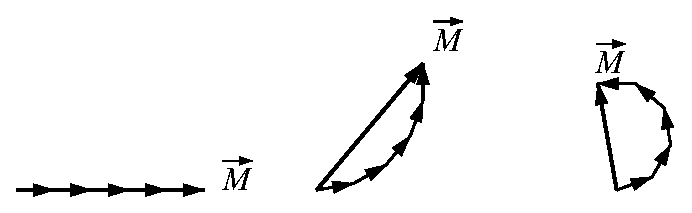
\epsfig{file=isochrom.eps,width=4in}
\end{center}
\caption{Effet de l'inhomogénéité de $\bzero$ sur l'évolution de l'aimantation transversale.}
\label{fig:isochrom}
\end{figure}

Expérimentalement on observe un affaiblissement de $\aimxys$ qui peut s'écrire
en première approximation par :
\begin{equation}
\aimxys (t) = \aimxys (t=0) . \exp \left( -\frac{t}{T_2^*} \right)
\end{equation}
où $T_2^*$ est le temps de relaxation transversal apparent, inférieur à $T_2$.

Indépendamment de $\aimxys$, $\aimzs$ évolue selon
\begin{equation}
\aimzs(t) = \aimzeros + (\aimzs (t=0) - \aimzeros)\exp \left( -\frac{t}{T_1} \right)
\end{equation}

Après une impulsion d'angle $\pi/2$, la composante longitudinale de $\aimvec$
est nulle et donc
\begin{eqnarray}
\label{eqn:relaxlong}
\aimzs(t) & = & \aimzeros \left( 1 - \exp \left( -\frac{t}{T_1} \right) \right) \\
\label{eqn:relaxtrans}
\aimxys(t) & = & \aimzeros \exp \left( -\frac{t}{T_2^*} \right)
\end{eqnarray}

Dans cette situation, la variation de $\aimzs$ et $\aimxys$ en fonction du temps 
est tracée figure \ref{fig:relax}.
En règle générale $T_2 \le T_1$.

\begin{figure}[hbt]
\begin{center}
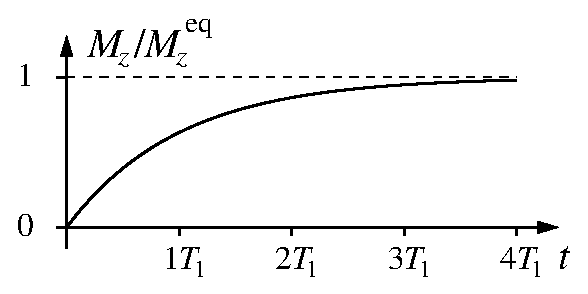
\epsfig{file=relaxlong.eps,width=2.5in}
\hspace{0.25in}
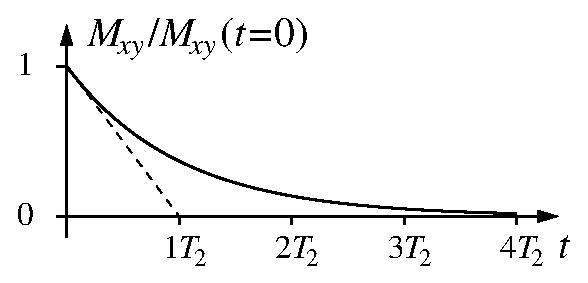
\epsfig{file=relaxtrans.eps,width=2.5in}
\end{center}
\caption{Relaxation longitudinale et transversale.}
\label{fig:relax}
\end{figure}

L'ordre de grandeur de $T_1$ et $T_2$ varie dans une gamme très large.
Il n'y a pas lieu de tenir compte de la relaxation pendant une impulsion de radio-fréquence
si $1/\omuns$ est faible par rapport aux temps de relaxation.
Les impulsions de grande durée et de faible intensité, voient leur efficacité modifiée par la
relaxation, donnant lieu au phénomène de saturation, qui ne sera pas étudié dans ce paragraphe.

Les expressions de $\aimxs (t)$ et de $\aimys (t)$ obtenues au paragraphe \ref{sec:larmor}
par résolution de l'équation du mouvement de $\aimvec$ dans le champ
$\bzerovec$ sont modifiées par la relaxation :
\begin{eqnarray}
\aimxs (t) & = & A\cos(\omega_0 t + \phi) \exp \left( -\frac{t}{T_2^*} \right) \\
\aimys (t) & = & A\sin(\omega_0 t + \phi) \exp \left( -\frac{t}{T_2^*} \right)
\end{eqnarray}

Le moment magnétique total d'un ensemble de noyaux est décrit d'une façon très
générale en tenant compte de l'action de $\bzerovec$, de l'action du champ de
radio-fréquence et des processus de relaxation.
Les équations différentielles qui résument l'effet de toutes ces
interactions sont désignées sous le nom d'équations de Bloch.

\section{Équations de Bloch}
\label{sec:eqnbloch}
Dans le référentiel tournant, l'équation \ref{eqn:blochrf2} décrit l'évolution
de $\aimvec$ sous l'action de $\bzerovec$ (modifiée par l'écran électronique)
et du champ de radiofréquence $\bunvec$, mais en l'absence de relaxation.
En considérant que la phase de $\bunvec$ est nulle, 
\begin{equation}
\omveceff = \left| \begin{array}{l}\omuns \\ 0 \\ \omzeros \end{array} \right.
\quad\mbox{et donc}\quad
\aimvec\wedge\omveceff = \left| \begin{array}{l} 
\aimys\omzeros \\ \aimzs\omuns-\aimxs\omzeros \\ -\aimys\omuns \end{array} \right.
\end{equation}
et vu que la relaxation agit aussi pendant l'application du champ $\bunvec$
selon les équations \ref{eqn:t1} et \ref{eqn:t2}, l'équation \ref{eqn:blochrf2}
devient :
\begin{eqnarray}
\derivt{\aimxs} & = & \aimys\omzeros - \frac{1}{T_2}\aimxs \\
\derivt{\aimys} & = & \aimzs\omuns-\aimxs\omzeros - \frac{1}{T_2}\aimys \\
\derivt{\aimzs} & = & -\aimys\omuns - \frac{1}{T_1} (\aimzs-\aimzerozs)
\end{eqnarray}
qui constituent les équations de Bloch.

Dans une expérience de RMN par impulsion et transformation de Fourier
utilisant des impulsions de RF brèves (quelques $\mu$s) par rapport à
$T_1$ et $T_2$ (au moins des ms, voire des secondes),
il est légitime d'ignorer l'effet de la relaxation pendant les impulsions.
La RMN par onde continue s'appuie sur la détection des états d'aimantation
qui correspondent à des solutions (quasi--)stationnaires des équations de Bloch.
Cet aspect de la RMN ne sera pas détaillé ici, sauf dans le cas
d'un champ $\bunvec$ appliqué en résonance ($\omzeros = 0$), car il aboutit
à la saturation de l'aimantation, utilisée pour l'établissement
de l'effet Overhauser nucléaire (section \ref{sec:noe}).
A l'état stationnaire, les coordonnées de $\aimvec$ sont indépendantes
du temps, Ainsi :
\begin{eqnarray}
0 & = & - \frac{1}{T_2}\aimxs \\
0 & = & \aimzs\omuns - \frac{1}{T_2}\aimys \\
0 & = & -\aimys\omuns - \frac{1}{T_1} (\aimzs-\aimzerozs)
\end{eqnarray}
dont la solution est :
\begin{eqnarray}
\aimxs & = & 0 \\
\aimys & = & \frac{\aimzerozs\omuns T_2}{1+\omuns^2 T_1 T_2} \\
\aimzs & = & \frac{\aimzerozs}{1+\omuns^2 T_1 T_2}
\end{eqnarray}

Si $\omuns \gg 1/\sqrt{T_1 T_2}$, alors $\aimzs \ll \aimzerozs$, ce qui
traduit une égalisation des populations des états $\al$ et $\be$ des spins nucléaires,
avec une disparition complète de l'aimantation macroscopique.

% \chapter[Signal]{Signal}

\section{Le signal de RMN}
La "mécanique" de l'aimantation décrite dans les paragraphes précédents montre
comment un échantillon dans son état d'équilibre magnétique est excité par une
impulsion de radio-fréquence et comment il revient vers son état initial en un
mouvement de précession de Larmor "amorti" par la relaxation.
L'utilisation de la RMN comme outil analytique nécessite la détermination
expérimentale du mouvement de l'aimantation.
Des résultats de cette mesure apparaissent les caractéristiques des
différentes populations de noyaux contenus dans l'échantillon.

La "bobine" qui transmet l'impulsion de courant de radiofréquence est à son
tour le siège d'une tension électrique alternative due au mouvement de
l'aimantation de l'échantillon.
Cette tension est appelée tension induite.
Dans un alternateur une partie mobile aimantée (rotor) tourne dans un
enroulement conducteur fixe (stator);
c'est très exactement de qui se passe en RMN où l'aimantation de l'échantillon
est mobile par rapport à la bobine fixe.
lorsque la bobine n'est plus utilisée pour transmettre
l'impulsion de radio-fréquence, la tension induite notée $e(t)$ est
enregistrée et analysée.
La tension induite est une grandeur physique mesurable dépendante du temps
définie pour $t \ge 0$,
l'instant $t = 0$ étant celui du début de son enregistrement.
L'expression "signal de RMN" ou "{\FIDfull}" ou "{\FID}"
(Free induction decay) désignera la fonction $e(t)$.

L'axe $Ox$ du référentiel du laboratoire a été choisi comme axe de la bobine au
paragraphe \ref{sec:macro}.
Le signal e(t) est créé par la variation de la projection de $\aimxs$ sur cet axe $Ox$ :
\begin{equation}
e(t) = K \derivt{\aimxs}
\end{equation}

Le nombre $K$ englobe un ensemble de facteurs géométriques liés à l'échantillon et à la
bobine, ainsi qu'un facteur lié au fait que la bobine est insérée dans
un circuit oscillant, circuit caractérisé par son facteur de surtension.
L'expression de $\aimxs(t)$ est
\begin{equation}
\aimxs(t) = A \cos(\omega_0 t + \phi) \exp(-t/T_2^*)
\end{equation}
dans l'hypothèse où un seul type de noyau est sollicité par l'impulsion de radio-fréquence.
Le facteur $A$ incorpore la valeur de l'aimantation d'équilibre $\aimzeros$ et le
facteur $\sin(\theta)$, où $\theta$ est l'angle de nutation (voir équation \ref{eqn:pulseaction}).
L'expression de $e(t)$ s'en déduit par dérivation :
\begin{equation}
e(t) = K A \exp(-t/T_2^*) (\omega_0 \sin(\omega_0 t + \phi) -
1/T_2^* \cos(\omega_0 t + \phi) )
\end{equation}

$e(t)$ est la somme de deux fonctions sinusoïdales amorties, l'une proportionnelle à
$\omega_0$, et l'autre à $1/T_2^*$, de plusieurs ordres de grandeur
inférieur à la première.
Le second terme est toujours négligeable devant le premier et donc :

\begin{equation}
e(t) = \emax \exp(-t/T_2^*) \sin(\omega_0 t + \phi)
\end{equation}

Formellement le signal $e(t)$ et l'aimantation $\aimxs(t)$ ont des expressions identiques,
à une différence de phase près.
Ces deux grandeurs seront souvent confondues par la suite bien qu'en réalité la première soit
la dérivée de la seconde par rapport au temps.
Ceci n'est possible qu'à cause de la
relative lenteur du phénomène de relaxation par rapport à la précession et à cause du
caractère sinusoïdal du signal.

Le paramètre le plus aisément modifiable par
l'expérimentateur est l'angle de l'impulsion de radiofréquence qui donne naissance au signal.
La composante horizontale $\aimxys$ de $\aimvec$ est maximale lorsque l'angle de l'impulsion est de
$\pi / 2$ ($\sin\theta=1$).
C'est donc à cette condition que l'amplitude du signal sera maximale,
en considérant que le signal ne provient que d'une seule séquence
impulsion--acquisition.
Dans une situation réelle où le rapport signal sur bruit est amélioré par
répétition de la séquence, il faut tenir compte de la vitesse de retour
de l'aimantation vers l'équilibre (donc des temps de relaxation) pour
choisir un angle de nutation optimal, angle qui est inférieur à $\pi/2$.

\section{Un récepteur très simplifié}
\label{sec:recept}

Toutes les fonctions d'un spectromètre par
impulsions et transformée de Fourier sont sous le contrôle d'un calculateur.
Cette nécessité s'est imposée par la nature de la chaîne de traitements qu'il faut faire subir au
signal $e(t)$ pour obtenir un spectre.
Un ensemble de traitements, comme l'amplification
et la démodulation (voir ci-après) sont du ressort de l'électronique analogique.

Le signal $e(t)$ a une fréquence égale à la fréquence de résonance des noyaux considérés,
qui se compte généralement en dizaines ou centaines de MHz.
S'il est techniquement
réalisable d'amplifier un tel signal (initialement de quelques $\mu$V), sa numérisation en
l'état n'est pas utile.

L'analyste désire en fait connaître la différence entre la fréquence de résonance des
noyaux étudiés et celle d'une substance de référence, différence qui donne accès aux
déplacements chimiques.
Ce qui est réalisé pratiquement par les circuits
électroniques de réception est une démodulation, opération qui
revient pratiquement à abaisser la fréquence du signal
d'une quantité égale à la fréquence des impulsions.
Le démodulateur livre un signal de basse fréquence $s(t)$ à partir du
signal $e(t)$ et de la tension délivrée par l'oscillateur qui pilote le générateur d'impulsion
(figure \ref{fig:spectroa}).
Le signal $s(t)$ est aussi appelé signal "audio--fréquence", par analogie à la
technique de réception radiophonique où le signal à transmettre est véhiculé par une
"onde porteuse" de haute fréquence puis démodulé (ou détecté) dans le récepteur.
A partir de
\begin{equation}
e(t) = A \exp(-t/T_2^*) \sin(\omega_0 t + \phi)
\end{equation}
le démodulateur fournit le signal $s(t)$ :
\begin{equation}
s(t) = A \exp(-t/T_2^*) \sin((\omega_0-\omrf) t + \phi)
= A \exp(-t/T_2^*) \sin(\omzeros t + \phi)
\end{equation}
où $\omzeros$ désigne la pulsation du signal d'audio--fréquence et $A$ son amplitude.
Le démodulateur abaisse la fréquence tout en conservant la phase du signal.
Il est indispensable de conserver l'information de la phase du signal dans $s(t)$ pour assurer,
entre autres choses, la possibilité d'augmentation du rapport signal/bruit par
accumulation.

La figure \ref{fig:spectroa} montre bien que le signal de référence ($\nuref = \omrf/2\pi$)
sert à la fois pour l'excitation de l'échantillon (il doit pour ce faire être amplifié
pour que ceci se déroule dans le temps le plus court possible) et pour la démodulation
du signal provenant de la sonde (c'est-à-dire de la partie du spectromètre qui 
entoure l'échantillon), signal qui doit être amplifié avant toute opération.
Le signal audio--fréquence est ensuite échantillonné (section \ref{sec:echantillon})
et numérisé par un convertisseur analogique-numérique (analog--digital converter, ou ADC) 
avant d'être traité par un calculateur (section \ref{sec:ft}).

\begin{figure}[hbt]
\begin{center}
\begin{pspicture}(0,1)(8.5,10.5)
\psset{linewidth=0.05}
\psframe(5.5,7.475)(6,10.5)
\psframe(5,7)(6.5,7.525)
\pscircle(5.5,7.25){0.1}
\pscircle(6,7.25){0.1}
\rput(4.75,7.75){Sonde}
\psframe(0,5.5)(1,6.5)
\rput(0.5,6){$\nuref$}
\psframe(3,5.5)(4,6.5)
\pspolygon(3.25,5.75)(3.75,6)(3.25,6.25)
\rput(3.5,6.75){Ampli.}
\psframe(7,5.5)(8,6.5)
\pspolygon(7.25,5.75)(7.75,6)(7.25,6.25)
\rput(7.5,6.75){Préampli.}
\psframe(7,4)(8,5)
\psline(7.25,4.25)(7.75,4.75)
\psline(7.75,4.25)(7.25,4.75)
\rput(5.75,4.75){Démodulateur}
\psframe(7,2.5)(8,3.5)
\rput(7.5,3){ADC}
\psframe(5,1)(8.5,2)
\rput(6.75,1.5){Calculateur}
\psline{->}(1,6)(3,6)
\psline(4,6)(5,6)(5.5,6.5)
\psline{<->}(5.5,6.5)(5.5,7)
\psline[linestyle=dashed,dash=5pt 5pt](5.5,6.5)(6,6)
\psline(6,6)(7,6)
\psline(8,6)(8.5,6)
\psline{->}(2,4.5)(7,4.5)
\psline{<-}(8,4.5)(8.5,4.5)
\psline(2,6)(2,4.5)
\psline(8.5,4.5)(8.5,6)
\psline{->}(7.5,4)(7.5,3.5)
\psline{->}(7.5,2.5)(7.5,2)
\end{pspicture}
\caption{\label{fig:spectroa}
\small Spectromètre très simplifié.}
\end{center}
\end{figure}

Il est commode de considérer que le démodulateur permet d'observer l'aimantation de
l'échantillon dans le référentiel tournant. Un signal $s(t)$ de fréquence nulle correspond à
la présence de noyaux exactement "en résonance" : $\omega_0 = \omrf$ et $\omzeros = 0$.
Un signal $s(t)$ de fréquence positive est dû à un noyau de fréquence de résonance
plus élevée que celle des impulsions.

Le schéma de détection du signal qui vient d'être présenté a l'inconvénient de fournir un
signal $s(t)$ où le signe de $\omzeros$ est ambigu.
Pour s'en rendre compte il suffit de considérer un premier signal
\begin{equation}
s_1(t)=A.\cos(\omzeros t + \phi).\exp(-t/T_2^*).
\end{equation}
Un autre noyau de pulsation de résonance $\omrf-\omzeros$ donnera un
signal
\begin{eqnarray}
s_2(t) & = & A.\cos(-\omzeros t + \phi).\exp(-t/T_2^*) \\
& = & A.\cos(\omzeros t - \phi).\exp(-t/T_2^*).
\end{eqnarray}
Dans l'expression de ces deux signaux apparaissent la même pulsation $\omzeros$ et des phases
opposées.
La phase n'étant pas connue de façon absolue, le signe de $\omzeros$ n'est pas
déterminé.
Un remède possible à cet état de fait consiste à choisir la fréquence des
impulsions en étant sûr qu'elle est soit supérieure (ou inférieure) à toutes les fréquences
de résonances présentées par les noyaux de l'échantillon ayant subi l'effet de
l'impulsion.

\section{La détection en quadrature}
Il ressort de l'analyse précédente qu'un schéma de détection monocanale (à
l'aide d'un seul démodulateur) ne peut pas donner accès au signe de $\omzeros$.
La technique de détection du signal dite "en quadrature" utilise deux démodulateurs, 
figure \ref{fig:spectrob}.
un premier démodulateur livre le signal $s_x(t)$, 
identique au signal $s(t)$ du paragraphe précédent.
La tension issue du circuit déphaseur est celle de l'oscillation pilote déphasée de 90$^{\circ}$.
Elle alimente le second démodulateur pour fournir le signal $s_y(t)$.
Les démodulateurs sont sensibles à la phase du signal qui les pilote, en conséquence :
\begin{eqnarray}
s_x(t) & = & A . \cos(\omzeros t + \phi) . \exp(-t/T_2^*) \\
s_y(t) & = & A . \sin(\omzeros t + \phi) . \exp(-t/T_2^*)
\end{eqnarray}
Si on porte dans un plan $XOY$ l'évolution du vecteur $\OMvec$ tel que
\begin{equation}
\OMvec = s_x(t) . \ivec + s_y(t) . \jvec
\end{equation}
on constate que ce vecteur retrace très exactement le mouvement de l'aimantation $\aimxyvec$
dans le référentiel tournant.
Le signe de $\omzeros$ est alors discernable sans ambiguïté.
Le traitement ultérieur des signaux $s_x(t)$ et $s_y(t)$, considérés simultanément, résout le
problème de la discrimination du signe de $\omzeros$.
Tout cela pour dire qu'il n'est pas possible de connaître le sens de rotation d'un objet
à partir de l'observation d'une seule projection de son mouvement et qu'il faut
deux projections pour y arriver.
Une manière commode de représenter le signal est de considérer la quantité complexe
\begin{equation}
s(t) = s_x(t) + is_y(t)
\end{equation}
qui contient toute l'information disponible sur l'aimantation transversale, à la
manière de $\OMvec$ mais en étant une quantité scalaire qui peut aussi s'écrire
\begin{equation}
\label{signalcomplexe}
s(t) = A . \exp(i(\omzeros t + \phi)) . \exp(-t/T_2^*)
\end{equation}
Le plan XOY du référentiel tournant est alors confondu avec le plan complexe comme 
l'indique la figure \ref{fig:xyplane}.

\begin{figure}[hbt]
\begin{center}
\begin{pspicture}(-4,-2)(4,2)
\SpecialCoor
\rput(-2.5,0){
\psline{->}(-1.5,0)(1.5,0)
\uput[0](1.5,0){$X$}
\psline{->}(0,-1.5)(0,1.5)
\uput[90](0,1.5){$Y$}
\uput[-135](0,0){$O$}
\psline{->}(0,0)(1,0)
\uput[-90](1,0){$\boldsymbol{\vec{\imath}}$}
\psline{->}(0,0)(0,1)
\uput[180](0,1){$\boldsymbol{\vec{\jmath}}$}
\psline[linewidth=0.05]{->}(0,0)(1.2;60)
\uput{2pt}[60](1.2;60){$\boldsymbol{\vec{M}}$}
}
\rput(2.5,0){
\psline(-1.5,0)(1.5,0)
\uput[0]{-90}(1.5,0){Réel}
\psline(0,-1.5)(0,1.5)
\uput[90]{0}(0,1.5){Imaginaire}
\uput[-135](0,0){$0$}
\psline(1,-0.1)(1,0.1)
\uput[-90](1,0){$\boldsymbol{1}$}
\psline(-0.1,1)(0.1,1)
\uput[180](0,1){$\boldsymbol{i}$}
\psline[linewidth=0.05]{->}(0,0)(1.2;60)
\uput{2pt}[60](1.2;60){$\boldsymbol{M}$}
}
\end{pspicture}
\caption{\label{fig:xyplane}
\small Plan transversal du référentiel tournant et plan complexe.}
\end{center}
\end{figure}

Une autre réalisation pratique de la
détection en quadrature est due à Redfield, mais le détail de son fonctionnement
nécessite la connaissance de l'échantillonnage du signal.

\begin{figure}[hbt]
\begin{center}
\begin{pspicture}(0,0)(8.5,10.5)
\psset{linewidth=0.05}
\psframe(5.5,7.475)(6,10.5)
\psframe(5,7)(6.5,7.525)
\pscircle(5.5,7.25){0.1}
\pscircle(6,7.25){0.1}
\rput(4.75,7.75){Sonde}
\psframe(0,5.5)(1,6.5)
\rput(0.5,6){$\nuref$}
\psframe(3,5.5)(4,6.5)
\pspolygon(3.25,5.75)(3.75,6)(3.25,6.25)
\rput(3.5,6.75){Ampli.}
\psframe(7,5.5)(8,6.5)
\pspolygon(7.25,5.75)(7.75,6)(7.25,6.25)
\rput(7.5,6.75){Préampli.}
\psframe(7,4)(8,5)
\psline(7.25,4.25)(7.75,4.75)
\psline(7.75,4.25)(7.25,4.75)
\rput(5.75,4.75){Démodulateur}
\psframe(5.5,3)(6.5,4)
\psline(5.75,3.25)(6.25,3.75)
\psline(6.25,3.25)(5.75,3.75)
\psframe(2.5,3)(4.5,4)
\rput(3.5,3.5){$\Delta\phi=90^{\circ}$}
\rput(3.5,2.75){Déphaseur}
\psframe(5.5,1.5)(6.5,2.5)
\rput(6,2){ADC}
\psframe(7,1.5)(8,2.5)
\rput(7.5,2){ADC}
\psframe(5,0)(8.5,1)
\rput(6.75,0.5){Calculateur}
\psline{->}(1,6)(3,6)
\psline(4,6)(5,6)(5.5,6.5)
\psline{<->}(5.5,6.5)(5.5,7.25)
\psline[linestyle=dashed,dash=5pt 5pt](5.5,6.5)(6,6)
\psline(6,6)(7,6)
\psline(8,6)(8.5,6)
\psline{->}(2,4.5)(7,4.5)
\psline{<-}(8,4.5)(8.5,4.5)
\psline{->}(2,6)(2,3.5)(2.5,3.5)
\psline{->}(4.5,3.5)(5.5,3.5)
\psline{<-}(6.5,3.5)(7.3,3.5)
\psline(7.7,3.5)(8.5,3.5)(8.5,6)
\psline{->}(6,3)(6,2.5)
\psline{->}(6,1.5)(6,1)
\psline{->}(7.5,4)(7.5,2.5)
\psline{->}(7.5,1.5)(7.5,1)
\end{pspicture}
\caption{\label{fig:spectrob}
\small Spectromètre utilisant la détection en quadrature.}
\end{center}
\end{figure}

\section{L'échantillonneur}
\label{sec:echantillon}
Le signal est une grandeur qui varie continûment au cours du temps.
Pour être traité par un calculateur numérique il faut l'échantillonner,
c'est à dire ne retenir du signal s(t)
qu'un nombre discret de valeurs (échantillons...), mesurées à des instants régulièrement
espacées.
Une "image" du signal est ainsi crée qui est d'autant plus fidèle au signal
d'origine que la fréquence des mesures est élevée.
En contrepartie, il y aura plus de valeurs de mesure à traiter et à stocker.
De plus, l'échantillonnage est d'autant plus délicat à
réaliser que sa fréquence est rapide.
A partir de la fonction $s(t)$ on construit une suite de
valeurs de tension $s_n$ telle que
\begin{equation}
s_n = s(n . \Delta t)
\end{equation}
où $n$ est le numéro de l'échantillon et $\Delta t$ le temps qui sépare deux mesures.
Les tensions $s_n$ sont ensuite converties en nombres binaires
par un convertisseur analogique-digital,
étape indispensable au traitement informatisé du signal.
Un grand nombre $N$ d'échantillons est ainsi mesuré,
$N$ étant généralement une puissance de 2.
L'inverse du temps qui sépare deux mesures définit la fréquence d'échantillonnage :
\begin{equation}
\nuech = \frac{1}{\Delta t}
\end{equation}
qui est le nombre de mesures effectuées en une seconde.
Le choix de $\nuech$ est déterminé par la
plus grande valeur de fréquence présente dans le signal, notée $\numax$ :
\begin{equation}
- \numax  < \frac{\omzeros}{2\pi} < + \numax
\end{equation}
Le théorème de Nyquist affirme qu'il faut que
\begin{equation}
\nuech = 2 . \numax
\end{equation}
Cela se justifie en considérant les signaux numérisés issus de deux signaux sinusoïdaux
de fréquence $\numax - \delta\nu$ et $\numax + \delta\nu$.
Un signal $s(t) = \cos(\omega t + \phi)$ se numérise en
$s_n = \cos(2\pi\nu n/2\numax + \phi)$ puisque $\Delta t = 1/2\numax$.

Si $\nu = \numax - \delta\nu$ alors
\begin{eqnarray}
s_n & = & \cos(2\pi n (\numax - \delta\nu)/2\numax + \phi) \\
& = & \cos(\pi n(1-\delta\nu/\numax) + \phi)
\end{eqnarray}

Si $\nu = \numax + \delta\nu$ alors
\begin{eqnarray}
s_n & = & \cos(2\pi n (\numax + \delta\nu)/2\numax + \phi) \\
& = & \cos(\pi n(1+\delta\nu/\numax) + \phi) \\
& = & \cos(\pi n(-1-\delta\nu/\numax) - \phi) \\
& = & \cos(2\pi n + \pi n(-1-\delta\nu/\numax) - \phi) \\
& = & \cos(\pi n(1-\delta\nu/\numax) - \phi)
\end{eqnarray}

\begin{figure}[hbt]
\begin{center}
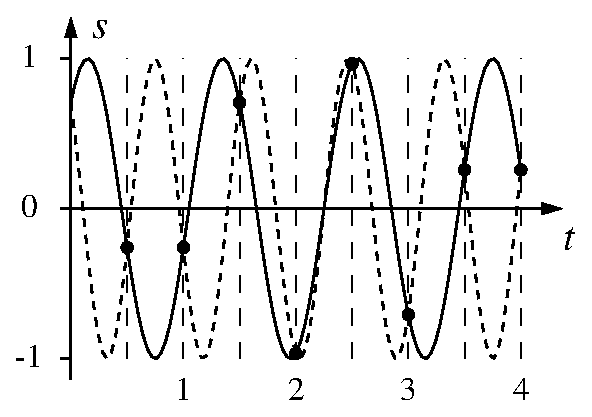
\epsfig{file=alias.eps,width=3in}
\end{center}
\caption{Illustration du phénomène de repliement spectral.}
\label{fig:aliasing}
\end{figure}

puisque $\cos(x+2\pi n) = \cos(x)$ et $\cos(x) = \cos(-x)$.
Les signaux numérisés sont donc indiscernables du point de vue de leur fréquence.
Un raisonnement général indique que tous les signaux de
fréquence $\nu$ tels que $\nu > \numax$ et $\nu < -\numax$ peuvent être considérés
après échantillonnage comme des signaux de fréquence comprise entre $-\numax$ et $+\numax$,
entraînant l'apparition d'informations erronées.
Ce phénomène porte le nom de
repliement spectral et est illustré figure \ref{fig:aliasing} 
où deux signaux de fréquences $\numax - \delta\nu$ et
$\numax + \delta\nu$ prennent des valeurs identiques à tous les instants d'échantillonnage.
Dans cette figure, $\numax = 1$ Hz et donc $\nuech = 2$ Hz, ce qui conduit à une
prise d'échantillons toutes les 0.5 s, matérialisée par les traits verticaux en pointillés fins
et les cercles.
Les signaux  représentés ont pour fréquence $1 - 1/6$ Hz (en trait plein) et
$1 + 1/6$ Hz (en pointillé). Leur échantillonnage conduit exactement
aux même mesures, ce qui prouve qu'ils seront vus de la même manière par
les traitement ultérieurs et conduiront à des spectres identiques.

Le cas qui vient d'être traité correspond à une détection du signal sur un seul canal,
cas dans lequel des signaux de fréquences opposés sont indiscernables.
La bande spectrale utile ne s'étend alors que de la fréquence 0 à la fréquence $\numax$,
soit une largeur spectrale de $\numax$.
La fréquence d'échantillonnage doit alors être le double de la largeur spectrale.
Dans le cas de la détection du signal complexe, la largeur spectrale $2\numax$ est égale
à la fréquence d'échantillonnage $2\numax$.
Deux signaux complexes de fréquences $\nu$ et $\nu+2\numax = \nu+\nuech$ sont 
en effet échantillonnés identiquement :
\begin{eqnarray}
s_n & = & \exp(i(2 \pi n (\nu + \nuech)/\nuech + \phi)) \\
& = & \exp(i(2 \pi n \nu/\nuech + 2 \pi n + \phi)) \\
& = & \exp(i(2 \pi n \nu/\nuech)).\exp(2 i \pi n) \\
& = & \exp(i(2 \pi n \nu/\nuech))
\end{eqnarray}.

Les signaux issus du repliement spectral 
sont de deux natures : il s'agit soit de signaux vrais 
(issus de l'échantillon) de fréquence trop
élevée soit de composantes du bruit de fond.
Un filtre dit "filtre audio" placé entre le démodulateur et l'échantillonneur
et dont la bande passante est légèrement supérieure à la largeur spectrale
voulue atténue ces signaux indésirables.

Les spectromètres modernes utilisent la technique du sur-échantillonnage dans
laquelle $\nuech$ est beaucoup plus grand que requis par le critère de Nyquist.
Le filtrage est alors réalisé par une technique numérique et non plus
par des composants analogiques.

\section{Le "Redfield trick"}
\label{sec:redfield}

Les signaux $s_x(t)$ et $s_y(t)$ issus du double démodulateur décrit figure
\ref{fig:spectrob} sont soit
échantillonnés simultanément (pour former le signal complexe), 
et on parlera de détection simultanée, soit échantillonnés
séquentiellement selon la méthode de Redfield.
Un système d'aiguillage électronique permet en fait de n'utiliser 
qu'un seul démodulateur et qu'un seul convertisseur, même pour
la détection simultanée.

Dans le cas de la détection séquentielle,
un seul signal réel est construit à partir de $s_x(t)$ et de $s_y(t)$
en intercalant un échantillon de $s_x(t)$ avec un de
$s_y(t)$ puis en changeant le signe des valeurs mesurées.
En supprimant comme au paragraphe précédent le terme
d'amplitude et de relaxation qui n'apportent rien à la compréhension de la méthode,
à partir de $s_x(t) = \cos(\omzeros t + \phi)$ et de $s_y(t) = \sin(\omzeros t + \phi)$
le signal échantillonné $s_n$ est tel
que :
\begin{eqnarray}
s_0 & = & +s_x(0 . \Delta t) = +\cos(\omzeros.0.\Delta t + \phi) \\
s_1 & = & -s_y(1 . \Delta t) = -\sin(\omzeros.1.\Delta t + \phi) \\
s_2 & = & -s_x(2 . \Delta t) = -\cos(\omzeros.2.\Delta t + \phi) \\
s_3 & = & +s_y(3 . \Delta t) = +\sin(\omzeros.3.\Delta t + \phi) \\
s_4 & = & +s_x(4 . \Delta t) = +\cos(\omzeros.4.\Delta t + \phi) \\
\mbox{etc...} & &
\end{eqnarray}
L'expression de $s_0$ .... $s_4$ se réécrit  :
\begin{eqnarray}
s_0 =  \cos(\omzeros.0.\Delta t + 0 . \pi/2 + \phi) \\
s_1 =  \cos(\omzeros.1.\Delta t + 1 . \pi/2 + \phi) \\
s_2 =  \cos(\omzeros.2.\Delta t + 2 . \pi/2 + \phi) \\
s_3 =  \cos(\omzeros.3.\Delta t + 3 . \pi/2 + \phi) \\
s_4 =  \cos(\omzeros.4.\Delta t + 4 . \pi/2 + \phi) \\
\mbox{etc...} & &
\end{eqnarray}
Si $\Delta t$ est choisi maintenant comme $1/4\numax$, c'est-à-dire si la fréquence
d'échantillonnage est double de celle utilisée en détection simultanée, 
le signal $s(t)$ qui
donnerait $s_n$ une fois échantillonné s'écrit en remplaçant $n$ par $t/\Delta t$.
\begin{eqnarray}
s(t) & = & \cos(2\pi\nu_0 t + t.4\numax.\pi/2 + \phi) \\
     & = & \cos(2\pi(\nu_0 + \numax)t + \phi)
\end{eqnarray}
On constate que ceci revient à augmenter la phase $\phi$ d'une quantité
proportionnelle au temps.
Puisque $\numax$ est par définition la fréquence la plus élevée du signal,
la quantité $\nu_0 + \numax$ est toujours positive.
Le signal $s(t)$ construit par la méthode de Redfield ne
contient que des signaux de fréquence positive et le problème de la détermination du
signe de $\nu_0$ (ou de $\omzeros$) ne se pose plus.
Lorsque la fréquence des impulsions est choisie
de façon à ce que les signaux $s_x(t)$ et $s_y(t)$ aient une fréquence comprise entre
$-\numax$ et $+\numax$,
(on dira : "la porteuse est au milieu du spectre") la méthode de "préparation" de
$s(t)$ décale toutes les fréquences de la quantité $\numax$.
Le critère de Nyquist impose donc le
doublement de la fréquence d'échantillonnage ($\Delta t = 1/4\numax$) puisque les fréquences
intervenant dans $s(t)$ sont comprises entre 0 et $2.\numax$.

La façon dont $s(t)$ est construit par la méthode de Redfield
est en fait une mesure de $\aimvec$ sur un axe $OR$ mobile par
rapport au référentiel tournant.
$\aimvec$ est successivement mesuré sur les axes :
\begin{eqnarray}
+OX		& \mbox{au temps} &		0 \\
-OY		& &			1/4\numax \\
-OX		& &			2/4\numax \\
+OY		& &			3/4\numax \\
+OX		& &			4/4\numax \\
\mbox{etc...}& &
\end{eqnarray}
L'axe $OR$ sur lequel $\aimvec$ est mesuré fait donc un tour en un temps $4/4\numax$,
sa fréquence de rotation par rapport au référentiel tournant est donc $\numax$,
dans le sens négatif de rotation.
Tout vecteur tournant à une fréquence $\nu$ supérieure à $-\numax$ par rapport au
référentiel tournant (cela doit être le cas de tous les vecteurs $\aimvec$) apparaîtra 
bien comme
tournant à une fréquence positive par rapport à l'axe OR.

\section{Analyse harmonique et linéarité}
\label{sec:ft}
Après démodulation en quadrature et échantillonnage le spectromètre délivre soit un 
ensemble de signaux $s_x(t)$ et $s_y(t)$ sous forme d'un signal complexe
si la détection est simultanée soit un signal réel unique $s(t)$ 
si la méthode de détection de Redfield est employée. 
Ces signaux proviennent du retour 
à l'équilibre d'un ensemble de noyaux préalablement excités par une impulsion de 
radio-fréquence. 
La  question à résoudre par l'analyste est : combien de type de noyaux résonnent à quelle 
fréquence? 
Répondre à cette question revient à élaborer un graphique portant en 
abscisse des fréquences et en ordonnée une amplitude qui caractérise le nombre de 
noyaux résonnant à chaque fréquence. 
Un tel graphique est un spectre, représentation 
d'une fonction notée $S(\Oms)$. 
Le but de l'analyse harmonique est la transformation d'un 
signal $s(t)$, fonction du temps, 
en une fonction de la pulsation (ou de la fréquence) $S(\Oms)$ 
qui caractérise le "contenu sinusoïdal" du signal.

Jusqu'ici seul des ensembles de noyaux identiques ont été considérés pour établir 
l'expression de $e(t)$, $s(t)$ et $s_n$. 
Ces noyaux sont caractérisés par leur pulsation 
propre $\omzeros$, leur temps de relaxation transversal apparent $T_2^*$, 
et leur aimantation initiale $\aimzerovec$. 
Les opérations qui mènent de $\aimvect$ à $s_n$ sont linéaires (si elles sont effectivement 
réalisées de façon idéale) c'est à dire que le résultat ($s_n$) obtenu en considérant plusieurs 
populations de noyaux est celui qui serait obtenu en faisant la somme des résultats 
individuels obtenus à partir des différentes populations prises séparément. 
Plus formellement une opération $O$ qui agit sur deux objets $x_1$ et $x_2$ 
(vecteurs, fonctions...) est linéaire si :
\begin{eqnarray}
O(x_1 + x_2) & = & O(x_1) + O(x_2) \\
O(\lambda . x_1) & = & \lambda . O(x_1)
\end{eqnarray}
L'aimantation totale d'un ensemble de deux noyaux est la somme de leurs aimantations 
individuelles. 
Sous réserve que l'impulsion soit non sélective, l'amplitude de 
l'aimantation transversale se déduit de l'angle de nutation de 
l'impulsion de façon identique pour les 
différentes populations de noyaux. 
Le passage de l'aimantation 
transversale vers le signal $e(t)$ fait intervenir une dérivation par rapport au temps, 
opération qui est linéaire : la dérivée d'une somme de fonctions est la somme de leurs 
dérivées. 
Les étapes d'amplification, de démodulation et d'échantillonnage sont linéaires 
dans la mesure où leur réalisation pratique est infiniment parfaite... 
Fondamentalement la conversion analogique-numérique est nécessairement une étape non linéaire 
puisqu'un il faut que le signal atteigne au moins une valeur de seuil (non nulle) pour 
que le convertisseur donne autre chose que la valeur numérique nulle. 
D'un point de vue pratique la "numérisation" du signal est considérée comme linéaire 
si la valeur de seuil est très faible,
c'est-à-dire si la taille du nombre binaire fournie est grande. 

L'opération qui transforme le signal numérisé en spectre numérisé est une opération 
linéaire, réalisée par différentes méthodes de calcul numérique. 
Parmi ces méthodes la Transformation de Fourier est actuellement la plus répandue, 
essentiellement à cause de sa très grande vitesse d'exécution. 
La linéarité de la transformation de Fourier nous autorise à poursuivre le 
cheminement du signal en ne considérant qu'une seule population de noyaux identiques.

\section{La transformation de Fourier (TF) réelle}
Appliquer la transformation de Fourier réelle (réelle, par opposition à complexe) à un 
signal, c'est faire implicitement l'hypothèse que ce signal est une fonction du temps à 
valeurs réelles qui s'écrit comme une somme de fonctions sinusoïdales d'amplitudes et de 
phases à déterminer pour chaque fréquence (ou pulsation) possible. 
Dans un cas général il ne s'agit pas d'une somme 
discrète mais d'une superposition continue de sinusoïdes :
\begin{equation}
s(t) = \intmp A(\Oms) \cos(\Oms t + \phi(\Oms)) \, d\Oms
\end{equation}
Une sinusoïde amortie, par exemple, ne peut pas en toute rigueur s'écrire comme une 
somme de sinusoïdes pures en nombre fini. 
En développant l'expression de $s(t)$ sous la 
forme :
\begin{equation}
s(t) = \intzp R(\Oms) \cos\Oms t \, d\Oms + \intzp I(\Oms) \sin\Oms t \, d\Oms
\end{equation}
le terme de phase $\phi(\Oms)$ est englobé dans les fonctions $R(\Oms)$ et $I(\Oms)$. 
On peut montrer que : 
\begin{eqnarray}
\label{eqn:ftftr}
R(\Oms) & = & \intzp s(t).\cos \Oms t \, dt \\
\label{eqn:ftfti}
I(\Oms) & = & \intzp s(t).\sin \Oms t \, dt
\end{eqnarray}
en toute rigueur des facteurs multiplicatifs doivent figurer devant les expressions de 
$R(\Oms)$ et de $I(\Oms)$ mais ils n'apportent pas de modification au raisonnement. 
Une justification de ces expressions est donnée dans l'appendice \ref{chap:fourier}.

Dans un premier temps nous allons considérer que $s(t)$ provient de l'évolution libre d'un 
seul type de noyau et que le facteur de phase est nul : 
$s(t) = \cos \omzeros t . \exp(-t/\lambda_0)$. 
L'évaluation de $R(\Oms)$ et de $I(\Oms)$ s'obtient en calculant :
\begin{eqnarray}
R(\Oms) & = & \intzp  \cos\Oms t . \cos \omzeros t . \exp(-t/\lambda_0) \, dt \\
\mbox{et}\quad	
I(\Oms) & = & \intzp  \sin\Oms t . \cos \omzeros t . \exp(-t/\lambda_0) \, dt
\end{eqnarray}
Les calculs sont simplifiés en considérant que :
\begin{eqnarray}
\intzp \cos \Oms t . \exp(-t/\lambda_0) \, dt & = & \lambda_0/(1 + \lambda_0^2 \Oms^2) \\
\mbox{et}\quad
\intzp \sin \Oms t . \exp(-t/\lambda_0) \, dt & = & \Oms\lambda_0^2/(1 + \lambda_0^2 \Oms^2)
\end{eqnarray}
Sachant que
\begin{equation}
\cos \Oms . \cos \omzeros = \cos(\Oms - \omzeros) + \cos(\Oms + \omzeros), 
\end{equation}
à un facteur 2 près (sans importance) on déduit :
\begin{equation}
R(\Oms) = \lambda_0/(1 + (\Oms - \omzeros)^2\lambda_0^2) + 
\lambda_0/(1 + (\Oms + \omzeros)^2\lambda_0^2)
\end{equation}
Les deux termes sont semblables et changer $\omzeros$ en $-\omzeros$ 
donne la même valeur de $R(\Oms)$. 
La fonction
\begin{equation}
A(\Oms) = \lambda_0/(1 + (\Oms - \omzeros)^2\lambda_0^2)
\end{equation}
est appelée fonction de Lorentz  en absorption et sa représentation graphique, figure \ref{fig:absorp}, 
est la courbe lorentzienne $A(\Oms)$, centrée sur $\Oms = \omzeros$, ayant en ce point sa valeur maximale $\lambda_0$. 
Sa largeur à mi-hauteur vaut $2/\lambda_0$, elle est matérialisée par les points $A$ et $B$.
La fonction représentée est en fait $A(\Oms)/\lambda$ dont le maximum
est toujours égal à 1.

\begin{figure}[hbt]
\begin{center}
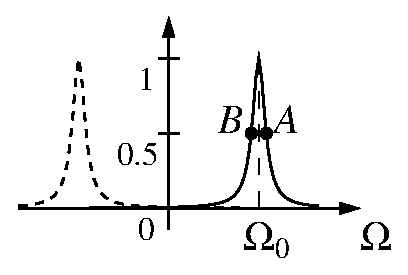
\epsfig{file=absorp.eps,width=2in}
\end{center}
\caption{\label{fig:absorp}Fonction de Lorentz (absorption).}
\end{figure}

Les fonctions de Lorentz centrées sur 
$\Oms = \omzeros$ seront notées $A(\omzeros)$, 
bien qu'il s'agisse implicitement d'une fonction de la variable $\Oms$ 
dont $\omzeros$ est un paramètre. 
Dans le cas étudié :
\begin{equation}
R(\Oms) = A(\omzeros) + A(-\omzeros)
\end{equation}
La courbe en pointillé sur la figure \ref{fig:absorp} est centrée autour
de $-\omzeros$ ; sa contribution à la partie du spectre où $\Oms \ge 0$ est pratiquement
négligeable.

Suivant des calculs analogues
\begin{eqnarray}
I(\Oms) & = & D(\omzeros) + D(-\omzeros) \\
\mbox{où}\quad D(\omzeros) & = & \lambda_0^2(\Oms - \omzeros)/
(1 + (\Oms - \omzeros)^2\lambda_0^2) 
\end{eqnarray}
La fonction $D(\Oms)$ est la fonction de Lorentz en dispersion.
Les représentations graphiques de $D(\Oms)/\lambda$ (trait plein)
et de $D(-\omzeros)/\lambda$ (trait pointillé) sont données 
figure \ref{fig:dispers}.
Les valeurs du maximum et du minimum sont respectivement 0.5 et -0.5 et leur
écartement en fréquence vaut $2/\lambda$.
La largeur à mi-hauteur est donc nécessairement plus grande que celle
de la courbe d'absorption.

\begin{figure}[hbt]
\begin{center}
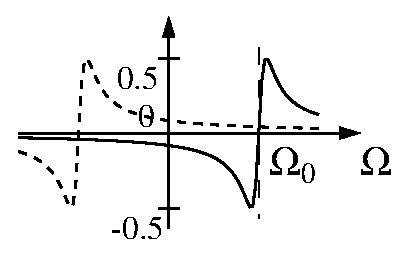
\epsfig{file=dispers.eps,width=2in}
\end{center}
\caption{\label{fig:dispers}Fonction de Lorentz (dispersion).}
\end{figure}

Les transformées de Fourier réelles $R(\Oms)$ et $I(\Oms)$ 
ne se calculent qu'à partir de signaux (réels) où toutes les 
fréquences sont censées être du même signe, puisqu'elles ne s'applique qu'à un seul 
signal (voir section \ref{sec:recept} et \ref{sec:redfield}).
On ne conserve généralement de $R(\Oms)$ et de $I(\Oms)$ que la partie 
correspondant aux fréquences positives. 
Dans la mesure où les raies spectrales ont une largeur faible par rapport à
la largeur spectrale totale et où les raies ne sont pas
trop proches des bords du spectres, les contributions de $A(-\omzeros)$ et de 
$D(-\omzeros)$ sont négligeables et on peut donc considérer que 
$R(\Oms) = A(\omzeros)$ et que $I(\Oms) = D(\omzeros)$,
ce qui est plus vrai pour $A(\Oms)$ que pour $D(\Oms)$, comme il
est possible de se rendre compte en comparant les figures
\ref{fig:absorp} et \ref{fig:dispers}, tracées avec des paramètres identiques.

Le spectre $S(\Oms)$ usuellement présenté à l'analyste est la représentation de la fonction 
$A(\Oms)$, dite courbe en Absorption pure. 
La fonction $D(\Oms)$ n'est en général pas 
représentée.
La fonction $D(\Oms)$ est en effet intrinsèquement plus large que $A(\Oms)$
ce qui rend plus difficile la distinction entre deux raies de fréquences proches,
entre autres inconvénients.

Dans l'exemple qui vient d'être traité, où la phase du signal est nulle, 
les fonctions $R(\Oms)$ et $A(\Oms)$ d'une 
part et $I(\Oms)$ et $D(\Oms)$ d'autre part sont identiques. 
Il n'en est pas de même lorsque la phase du signal n'est pas nulle. 
Pour obtenir un spectre où toutes les raies sont des 
courbes en absorption pure il faut nécessairement appliquer un
traitement à $R(\Oms)$ et $I(\Oms)$, le phasage.
Avant d'aborder cette question, regardons le sens physique du résultat qui vient d'être obtenu.

Un signal $s(t)$, produit d'une fonction sinusoïdale
de phase nulle et de pulsation $\omzeros$ par 
un facteur d'amortissement se décompose comme une somme d'une infinité de 
sinusoïdes de pulsations voisines de $\omzeros$. 
Moins ce signal est amorti, c'est-à-dire plus $\lambda_0$ est grand, 
et moins il y a de "participation" des sinusoïdes de fréquence éloignées de $\omzeros$ 
dans le signal. 
A l'extrême limite, si le signal est une sinusoïde pure, $S(\Oms)$ est 
une fonction nulle partout sauf pour $\Oms = \omzeros$ où elle prend une valeur infinie. 
La surface située sous la courbe en absorption ne dépend pas 
du facteur d'amortissement : diviser 
$\lambda_0$ par 2 double la largeur de la raie et divise par deux sa hauteur. 
La surface de la raie en absorption contient donc l'information quantitative 
que l'on peut tirer de la RMN : 
il est possible de tirer d'un spectre les populations relatives des différents types de noyaux 
de l'échantillon en faisant le rapport des surfaces des pics d'absorption correspondants. 
Les programmes de traitement des spectres permettent le calcul de ces surfaces relatives 
par intégration numérique de parties de spectres. 
Cela n'est pas le seul intérêt de la présentation des spectres en absorption : 
comme l'indiquent les figures \ref{fig:absorp} et \ref{fig:dispers}, les raies 
d'absorption sont, toutes choses égales par ailleurs, moins large que les raies en 
dispersion, amenant par là-même une sensible amélioration de la résolution des 
spectres. 
La présence de la fonction $I(\Oms)$ se justifie par la nature causale du signal : il 
n'est défini que pour $t \ge 0$ ; son calcul se justifie lorsqu'il y a lieu de phaser les spectre.

Si maintenant le signal contient un terme de phase : 
\begin{eqnarray}
s(t) & = & \cos (\omzeros t + \phi). \exp(-t/\lambda_0) \\ 
& = & \cos \omzeros t . \cos \phi . \exp(-t/\lambda_0) - 
\sin \omzeros t . \sin \phi . \exp(-t/\lambda_0)
\end{eqnarray}
le calcul de $R(\Oms)$ et de $I(\Oms)$ 
nécessite l'établissement des résultats suivants :
\begin{eqnarray}
\intzp  \cos \Oms t . \sin \omzeros t . \exp(-t/\lambda_0) \, dt & = &
D(\omzeros) - D(-\omzeros) \\
\mbox{et}\quad
\intzp  \sin \Oms t . \sin \omzeros t . \exp(-t/\lambda_0) \, dt & = &
A(\omzeros) - A(-\omzeros)
\end{eqnarray}
En ne gardant que la partie où $\Oms$ est positif dans $R(\Oms)$ et $I(\Oms)$ :
\begin{eqnarray}
R(\Oms) & = & A(\omzeros) . \cos \phi - D(\omzeros) . \sin \phi \\
\mbox{et}\quad 
I(\Oms) & = & A(\omzeros) . \sin \phi + D(\omzeros) . \cos \phi
\end{eqnarray}
La valeur de la phase étant a priori indéterminée $R(\Oms)$ et $I(\Oms)$ sont généralement des 
combinaisons de raies en absorption et en dispersion. 
Des spectres en absorption pure $S_A(\Oms)$ et $S_D(\Oms)$ sont calculables à partir de 
$R(\Oms)$ et de $I(\Oms)$ :
\begin{eqnarray}
S_A(\Oms) & = & R(\Oms) . \cos \phi + I(\Oms) . \sin \phi = A(\omzeros) \\
S_D(\Oms) & = & I(\Oms) . \cos \phi - R(\Oms) . \sin \phi = D(\omzeros)
\end{eqnarray}
Le spectre $S(\Oms)$ recherché est $S_A(\Oms)$, 
le spectre en dispersion pure est calculé pour 
permettre un phasage ultérieur si la valeur de $\phi$ choisie n'est pas correcte. 
La phase de tous les signaux issus d'un même échantillon serait identique si 
l'acquisition du signal commençait juste après l'impulsion. 
Cette commutation infiniment rapide n'est pas 
réalisable techniquement et un délai d'attente est nécessaire entre l'émission d'une 
impulsion et la réception du signal. 
Pendant ce délai les différentes composantes du 
signal se déphasent les unes des autres d'un angle égal au produit de leur pulsation par la 
durée du délai, ce qui aboutit à une dépendance linéaire entre $\phi$ et $\omzeros$ :
$\phi(\Oms) = a\Oms + b$.
L'opération qui consiste à trouver les paramètres $a$ et $b$ tels que 
$S_A(\Oms)$ ne présente que des raies en absorption
pure sur l'ensemble des raies du spectre est appelée phasage du spectre.
Les effets d'offset introduisent aussi une dépendance entre $\phi$ et $\omzeros$,
qui pratiquement peut être considérée comme linéaire.
Le phasage d'un spectre est effectué par le logiciel des spectromètres de 
manière interactive (l'utilisateur décide si les valeurs de $a$ et de $b$
conduisent à des raies spectrales symétriques par rapport à leur maximum)
ou de manière automatique. 

Une possibilité pour obtenir des raies spectrales symétriques 
consiste à calculer soit $P(\Oms)$ soit $M(\Oms)$ :
\begin{eqnarray}
P(\Oms) & = & R(\Oms)^2 + I(\Oms)^2 = A(\omzeros)^2 + D(\omzeros)^2 \\
M(\Oms) & = & P(\Oms)^{1/2} 
\end{eqnarray}
Ces spectres sont appelés respectivement spectres en puissance et en magnitude, ils sont 
indépendants de la phase du signal. 
Ils présentent tous les deux des raies plus larges que 
les raies en absorption.

Le spectre en puissance favorise les grands pics au détriment des 
petits, laissant une apparence spectre moins "bruyant", 
au détriment de l'information quantitative.
Une raie d'un spectre en puissance possède la forme d'une raie en absorption pure.
Il en résulte que la largeur à mi-hauteur d'une raie en magnitude (de forme non-lorentzienne)
est égale à la largeur à quart de hauteur de la raie en absorption : $2\sqrt{3}/\lambda$.

En résumé, si le signal à traiter est un signal réel issu soit d'une démodulation 
monocanale, soit du "Redfield trick", sa transformée de Fourier est constituée d'une 
paire de fonctions $R(\Oms)$ et $I(\Oms)$ 
dont on ne garde que les valeurs définie pour $\Oms$ positif. 
L'hypothèse de la présence de composantes du signal de fréquences de signes tous identiques 
est nécessaire pour obtenir un résultat pertinent. 
Un spectre de raies en absorption pure s'obtient par phasage, c'est-à-dire par
combinaison des fonctions $R(\Oms)$ et $I(\Oms)$.

\section{Transformation de Fourier complexe}

La méthode de double démodulation et d'échantillonnage simultané produit les signaux 
$s_x(t)$ et $s_y(t)$ qui traduisent le mouvement de $\aimvec$ par rapport aux axes $OX$ et $OY$ du 
référentiel tournant. 
Leur analyse harmonique simultanée par transformation de Fourier 
va nécessairement être exécutée autrement que s'il s'agissait d'un unique signal, issu de 
la méthode de Redfield par exemple.
La transformation de Fourier complexe, en considérant
simultanément l'évolution de l'aimantation nucléaire sur deux axes
orthogonaux du référentiel tournant, est capable de distinguer des 
fréquences d'évolution positives ou négatives du signal, superposition de
signaux élémentaires $\exp(i \Oms t)$ couvrant a priori tout l'éventail possible
des fréquences :
\begin{equation}
s(t) = \intmp S(\Oms).\exp(i \Oms t) \, d\Oms
\end{equation}

Pour un signal provenant d'un unique type de noyaux, 
considérons à nouveau le signal complexe présenté dans l'équation \ref{signalcomplexe},
mais avec les notations du paragraphe précédent :
\begin{eqnarray}
s(t) & = & 
\cos (\omzeros t + \phi) . \exp(-t/\lambda_0)) 
+ i.\sin (\omzeros t + \phi) . \exp(-t/\lambda_0)) \\
& = & \exp(i \omzeros t) . \exp(-t/\lambda_0) . \exp(i\phi)
\end{eqnarray}
Un premier intérêt à la manipulation d'un signal complexe se manifeste en
constatant que la phase intervient dans un coefficient multiplicatif
du signal, coefficient qui se retrouver inchangé dans l'expression
du spectre complexe qui sera obtenu, et ceci par linéarité de la TF.
Il sera commode dans un premier temps de considérer un signal de phase nulle.

La transformée de Fourier complexe 
$S(\Oms)$ du signal complexe $s(t)$ est définie par :
\begin{equation}
\label{eqn:ftcomplexe}
S(\Oms) = \intzp s(t) . \exp(-i \Oms t) \, dt
\end{equation}
C'est une fonction à valeurs complexes dont les parties réelles
et imaginaires sont notées maintenant $R_C(\Oms)$ et $I_C(\Oms)$.
La justification de l'équation \ref{eqn:ftcomplexe} est donnée dans
l'annexe \ref{chap:fourier}.

Si le signal est de phase nulle :
\begin{eqnarray}
s(t) & = & \exp(i \omzeros t) . \exp(-t/\lambda_0) \\
& = & \cos(i \omzeros t) . \exp(-t/\lambda_0) + i\sin(i \omzeros t) . \exp(-t/\lambda_0) \\
& = & s_x(t) + i.s_y(t)
\end{eqnarray} 
alors 
\begin{eqnarray}
S(\Oms) & = & \intzp (s_x(t)+is_y(t)(\cos \Oms t - i \sin \Oms t) \, dt \\
& = & R_C(\Oms) + iI_C(\Oms)
\end{eqnarray}
avec, en développant et en regroupant les parties réelles et imaginaires
\begin{eqnarray}
R_C(\Oms) & = & \intzp s_x(t)\cos\omzeros t + s_y(t)\sin\omzeros t \, dt \\
\mbox{et}\quad
I_C(\Oms) & = & \intzp -s_x(t)\sin\omzeros t + s_y(t)\cos\omzeros t \, dt
\end{eqnarray}
En utilisant les résultats du paragraphe précédent on obtient
\begin{eqnarray}
R_C(\Oms) & = & (A(\omzeros) + A(-\omzeros)) + (A(\omzeros) - A(-\omzeros))\\
I_C(\Oms) & = & (D(\omzeros) + D(-\omzeros)) + (D(\omzeros) - D(-\omzeros))
\end{eqnarray}
soit
\begin{equation}
S(\Oms) = A(\omzeros) + i.D(\omzeros)
\end{equation}
à un facteur 2 près.
Comme attendu, la fréquence $-\omzeros$ n'intervient plus dans l'expression
du spectre $S(\Oms)$.
Le signe - présent dans la définition de la TF complexe est nécessaire pour
obtenir ce résultat. 
Le changer en signe positif revient à changer $\omzeros$
en $-\omzeros$ dans l'expression de $S(\Oms)$.

Si de plus le signal comporte un facteur de 
phase $\exp(i\phi)$, sa transformée de Fourier complexe s'écrit :
\begin{eqnarray}
S(\Oms) & = & (A(\omzeros) + i.D(\omzeros)).(\cos\phi + i.\sin\phi) \\
& = & A(\omzeros).\cos\phi - D(\omzeros).\sin\phi + \\
& & i.(A(\omzeros).\sin\phi + D(\omzeros).\cos\phi ) \nonumber
\end{eqnarray}
On constate que la partie réelle (resp. imaginaire) de la transformée de Fourier 
complexe du signal complexe est identique à la fonction $R(\Oms)$ (resp. $I(\Oms)$) 
obtenue à partir du signal réel correspondant. 
A chaque mode de détection en quadrature correspond un mode de transformation de Fourier, 
le spectre obtenu étant ensuite manipulé (phasage, intégration...) exactement de la même manière. 
La technique utilisée pour la détection et la transformation du signal est 
généralement transparente à l'utilisateur. 
Il est néanmoins important d'avoir compris la différence entre les deux 
modes de transformation de Fourier pour analyser en RMN 2D le 
processus d'obtention et de phasage des spectres.

Même s'il faut être un peu familiarisé avec l'algèbre complexe, il est toujours plus 
pratique de désigner le signal et le spectre par une seule grandeur complexe plutôt que 
d'avoir à considérer séparément deux grandeurs réelles. 
Le formalisme de la matrice 
densité défini au chapitre suivant utilise de façon intensive les notions de signal et de spectre 
complexe. 
Dans l'expression du signal le facteur de relaxation sera souvent considéré comme implicite. 
Danc ce cas on écrira donc :
\begin{equation}
\exp(i \omzeros t) \xrightarrow{\mathrm{TF}} A(\omzeros) + i.D(\omzeros)
\end{equation}

\section{TF d'un signal échantillonné}
Les signaux et les spectres dont il a été question au paragraphe précédent
sont des fonctions de $t$ et de $\Oms$ où ces deux quantités varient
de manière continue.
Il a déjà été signalé qu'il n'est possible d'appréhender un signal temporel
que par son échantillonnage opéré à un nombre fini d'instants, si
les traitements qui lui sont ensuite appliqués sont effectués par un
calculateur numérique (un ordinateur).
Pour tenir compte de cette réalité, il est nécessaire de réécrire les relations
qui lient $s(t)$ et $S(\Oms)$ en faisant intervenir des sommes de nombres finis
de termes et non plus des intégrales.
Malgré l'intérêt théorique que cela représente, cet aspect ne sera pas développé
ici, et seuls les résultats utiles seront évoqués.

La transformation de Fourier, réelle ou complexe, est effectuée à partir
d'un nombre d'échantillons $N$ suivant un algorithme (une méthode de calcul)
dont le temps d'exécution croît comme la fonction $N\log(N)$, c'est-à-dire
reste utilisable pour toutes les valeurs de $N$ d'intérêt pratique,
pourvu que ce soit une puissance de 2.
Le résultat de la TF numérique est un spectre, lui-même
échantillonné dans le domaine des fréquences.
Un spectre tracé sur du papier n'est en fait défini que par un
nombre fini de points liés entre eux par des segments
de droite.

Pour des noyaux dont les fréquences de résonance sont réparties dans un intervalle
de largeur $\Delta\Oms$, entre $\omrf-\Delta\Oms/2$ et $\omrf+\Delta\Oms/2$,
deux schémas d'enregistrement des spectres sont possibles :
\begin{itemize}
\item
Le "Redfield trick" (ou détection séquentielle) est utilisé. 
Il faut alors échantillonner le signal à la fréquence $2\Delta\Oms$. 
Si $2N$ nombrés réels sont obtenus, la TF numérique réelle en donnera
deux fois $2N$ réels mais correspondant à une lageur spectrale
$2\Delta\Oms$, dont la moitié contiennent la même
information que l'autre moitié.
Il ne reste donc que $2N$ valeurs réelles utiles, $N$ pour $R(\Oms)$
et autant pour $I(\Oms)$.
Après phasage, le spectre utilisable (utilisé ?), ne contient que
des pics en absorption, et est constitué de $N$ valeurs.
\item
La détection simultanée est utilisée. 
La fréquence d'échantillonnage est alors $\Delta\Oms$. 
Si $N$ nombres complexes sont enregistrés (en fait $2N$ nombres réels, 
comme avec la détection séquentielle), la TF complexe produit $N$ nombres
complexes.
Après phasage du spectre, seule la partie réelle, constitué de $N$ valeurs,
est utilisée.
\end{itemize}

Les deux schémas sont largement équivalents et leur mise en {\oe}uvre
ne demande pas des moyens radicalement différents.
Au niveau du résultat, l'équivalence n'est cependant pas totale.
En effet les expressions de $R(\Oms)$ et $I(\Oms)$ font intervenir
les fonctions $A$ et $D$ avec comme paramètre $\omzeros$ et $-\omzeros$,
alors que $R_C(\Oms)$ et $I_C(\Oms)$ ne font intervenir que $\omzeros$.
Cela peut être mis en relation avec le fait que le repliement des signaux
dont la fréquence sort de la fenêtre spectrale choisie ne s'effectue
pas de la même manière dans les deux schémas.

L'analyse du procédé de FT numérique d'un signal échantillonné peut
néanmoins être poursuivie en ne considérant que la TF complexe. 
On désignera ainsi :
\begin{itemize}
\item $\delta t$ le temps qui sépare l'acquisition de deux échantillons,
\item $\Delta t$ le temps total de l'acquisition de $N$ valeurs complexes,
\item $\delta \Oms$ l'écart de fréquences entre deux points successifs du spectre
\item $\Delta \Oms$ la largeur spectrale.
\end{itemize}

Le critère de Nyquist indique que
\begin{equation}
\Delta \Oms . \delta t = 2\pi
\end{equation}
puisque la fréquence (et non pas la pulsation, d'où le terme $2\pi$)
d'échantillonnage est égale à la largeur spectrale.
Le temps total d'acquisition vaut $\delta t . N$ et l'écart
entre deux fréquences consécutives dans le spectre vaut
$\Delta \Oms/N$ puisque la TF complexe d'un signal contenant $N$
valeurs contient $N$ valeurs. Ainsi
\begin{equation}
\delta \Oms . \Delta t = 2\pi.
\end{equation}
La quantité $\delta\Oms$ est appelée résolution numérique du spectre
et est inversement proportionnelle à la durée de l'acquisition.

\section{Améliorer le rapport signal sur bruit}
Tout au long de la chaîne de traitement du signal analogique, un signal indésirable de 
caractère aléatoire se superpose au signal intéressant : le bruit. 
Son origine se trouve dans le caractère corpusculaire des électrons 
et dans leur "agitation" thermique. 
La tension induite dans la bobine est extrêmement faible et la perturbation 
apportée par le bruit est, dans le cas de noyaux peu sensibles ou peu nombreux, 
aussi grande voire plus grande que le signal issu de l'échantillon. 
Ce problème n'est pas typique de la RMN et sa solution 
réside dans plusieurs stratégies expérimentales. 
Il convient tout d'abord de disposer d'une sonde et de circuits d'amplification 
particulièrement soignés, et d'accorder au 
mieux la sonde, c'est-à-dire de faire en sorte que la transmission entre
la bobine et le préamplificateur à laquelle elle est connectée se fasse
avec un rendement maximum.

La différence fondamentale qui existe entre le signal vrai et le bruit est le caractère 
reproductible du premier et le caractère aléatoire du second. 
Par sommation de $M$ signaux obtenus dans des conditions identiques, 
l'amplitude du signal vrai est multipliée 
par $M$ et celle du bruit par $M^{1/2}$.

Ce dernier point mérite un développement et tout d'abord une définition de
ce qu'est l'amplitude du bruit.
Considérons un {\FID} constituée de $N$ valeurs réelles (pour simplifier)
constitués uniquement de bruit : $\epsilon_j (1 \le j \le N)$.
Idéalement, la moyenne des $\epsilon_j$ est nulle :
\begin{equation}
\frac{1}{N}\sum_{j=1}^{N} \epsilon_j = 0
\end{equation}
cette propriété restant valable quelque soit la collection,
suffisamment grande, d'échantillons de bruit.
La variance du bruit est alors définie comme la valeur quadratique moyenne
des écarts entre les échantillons et leur moyenne (nulle),
c'est-à-dire comme la moyenne des $\epsilon_j^2$, grandeur qui par définition
est strictement positive et d'autant plus grande que le bruit est "intense" :
\begin{equation}
\mbox{Var}(\epsilon) = \frac{1}{N}\sum_{j=1}^{N} \epsilon_j^2
\end{equation}
L'intensité du bruit est une grandeur physique de même dimension
que le bruit (des Volts, puisqu'il s'agit de mesurer une tension électrique)
et est définie comme la racine carrée de la variance :
\begin{equation}
\sigma(\epsilon) = \sqrt{\mbox{Var}(\epsilon)}.
\end{equation}

Sachant que $M$ {\FID} de $N$ valeurs chacune seront enregistrés, $\epsilon_{jk}$
désignera la valeur du $j\mieme$ échantillon 
du $k\mieme$ {\FID} et
$v_j$ la valeur du $j\mieme$ échantillon du signal "vrai", 
valeur qui ne dépend pas de $k$ puisqu'elle est reproductible.
En utilisant les mêmes notations, l'échantillon enregistré $s_{jk}$ s'écrit
\begin{equation}
s_{jk} = v_j + \epsilon_{jk}.
\end{equation}
et le signal $a$ résultant de l'addition de $M$ acquisitions est tel que
\begin{equation}
a_j = \sum_{k=1}^{M}(v_j + \epsilon_{jk}) = Mv_j + \sum_{k=1}^{M}\epsilon_{jk}.
\end{equation}
Le signal reproductible a bien été multiplié par $M$.
Le bruit $E$ présent dans ce signal est constitué des $E_j = a_j - Mv_j$, de valeur moyenne
nulle puisqu'elle est la somme de quantités de valeur moyenne nulle.
De plus,
\begin{eqnarray}
\mbox{Var(E)} 
& = & \frac{1}{N}\sum_{j=1}^N\left( \sum_{k=1}^M \epsilon_{jk} \right)^2 \\
& = & \frac{1}{N}\sum_{j=1}^N\left( \sum_{k=1}^M \epsilon_{jk}^2 +
\sum_{k=1}^M \sum_{\substack{l=1  \\ l \neq k}}^M \epsilon_{jk}\epsilon_{jl} \right) \\
\label{vara} & = & \sum_{k=1}^M \left( \frac{1}{N}\sum_{j=1}^N \epsilon_{jk}^2 \right) +
\sum_{k=1}^M \sum_{\substack{l=1 \\ l \neq k}}^M
\left( \frac{1}{N}\sum_{j=1}^N\epsilon_{jk}\epsilon_{jl} \right) \\
\label{varb} & = & M.\mbox{Var}(\epsilon)
\end{eqnarray}

Le passage entre les équations \ref{vara} et \ref{varb} mérite un commentaire.
On reconnaît aisément dans le premier terme de \ref{vara} la définition de 
$\mbox{Var}(\epsilon)$, valeur qui est sommée M fois à l'identique.
Le second terme de \ref{vara} fait intervenir le produit des bruits de deux
enregistrements, calculé échantillon par échantillon.
Comme les bruits issus de deux enregistrements différents ne sont pas corrélés
(au sens commun du terme comme au sens qu'en donne de manière rigoureuse la
théorie des statistiques), la moyenne de ces produits est nulle.

Ainsi,
\begin{equation}
\sigma(E) = \sqrt{M.\mbox{Var}(\epsilon)} = 
M^{1/2}.\sqrt{\mbox{Var}(\epsilon)} = M^{1/2}.\sigma(\epsilon)
\end{equation}
ce qui était le résultat annoncé.

Le rapport des intensités du signal et du bruit est donc multiplié par $M/M^{1/2}=M^{1/2}$. 
La durée d'enregistrement du signal de précession libre est relativement courte (de 
l'ordre de la seconde) ce qui permet l'accumulation rapide d'un grand nombre de 
signaux, le spectre étant obtenu après Transformée de Fourier du signal total. 
La TF étant une opération linéaire et la TF du bruit étant aussi du bruit, 
le rapport "spectre sur bruit",
aussi appelé rapport "signal sur bruit du spectre", est amélioré par le facteur $M^{1/2}$. 

La réalisation pratique de l'accumulation des signaux nécessite l'introduction d'un délai 
entre la fin de l'acquisition d'un signal et l'impulsion suivante est appelé délai de relaxation. 
Il est en effet indispensable de laisser à l'aimantation le temps de revenir aussi près que 
possible de son état initial. 
Si ce délai est trop bref la relaxation longitudinale n'a pas le 
temps de restaurer $\aimvec$ à sa valeur initiale et l'intensité des signaux dépendra des temps 
$T_1$ des différents types de noyaux de l'échantillon. 
Après quelques séquences excitation - 
acquisition - relaxation, l'aimantation "initiale" des noyaux devient reproductible car un 
état stationnaire s'établit progressivement. 
Lorsqu'une grande reproductibilité du signal 
est nécessaire (dans certaines expériences multi--impulsionnelles, par exemple) 
les premiers signaux ne sont pas enregistrés. 
Le temps total qui s'écoule entre deux 
séquences élémentaires est appelé temps de répétition.

L'amélioration du rapport S/B est réalisable sur un appareil à onde continue par 
accumulation de spectres. Un exemple numérique montre la supériorité de la RMN par 
impulsions dans ce domaine. Si on ne dispose que de 10 heures (36000 s) et que le 
temps de répétition est de 3.6 s il est possible de réaliser 10000 accumulations et donc 
d'améliorer le rapport S/B par un facteur 100. Si en onde continue il faut 6 minutes 
(360 s) pour enregistrer un spectre, seulement 100 spectres seront accumulés pendant le 
temps imparti, et l'amélioration du rapport S/B ne se fera que d'un facteur 10.

Une autre manière d'influencer le rapport signal sur bruit d'un spectre
est de faire subir un pré-traitement au signal temporel, appelé filtrage numérique,
juste avant d'effectuer la TF.

\section{Le filtrage numérique}
\label{filtrage}
Une étape intermédiaire entre la numérisation du signal et sa TF est parfois nécessaire 
afin d'en améliorer certaines caractéristiques et faciliter son exploitation. 
La multiplication du signal par une fonction appelée fonction "fenêtre" provoque une 
modification simultanée de la forme des raies et du rapport signal sur bruit
Le passage d'un signal analogique dans un filtre provoque une modification 
de son spectre, le  traitement qui donne le même type de modification, effectué sur un 
signal numérisé porte le nom de filtrage numérique.

\begin{figure}[hbt]
\begin{center}
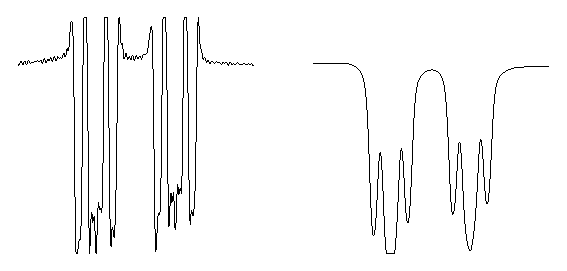
\epsfig{file=apodH.eps,width=3in,angle=180}
\end{center}
\caption[Effet du filtrage numérique sur un spectre du \prot.]
{Effet filtrage numérique sur un spectre du \prot.
A gauche, le spectre non filtré, et à droite filtré par un filtre de type
Lorentz-Gauss (rétrécissement des raies).}
\label{fig:apodH}
\end{figure}

La figure \ref{fig:apodH} montre comment 
la résolution d'un spectre de \prot à été artificiellement améliorée au dépend 
du rapport S/B et de la forme des raies.
Dans le spectre de \carb de la figure \ref{fig:apodC}, le rapport S/B
a été amélioré au dépend de la largeur des raies.

\begin{figure}[hbt]
\begin{center}
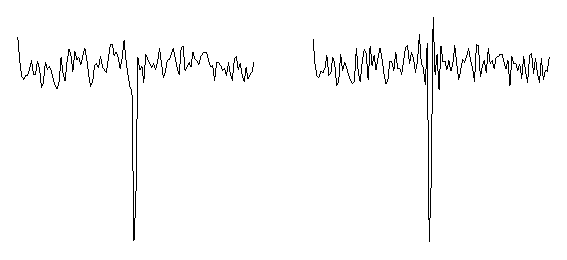
\epsfig{file=apodC.eps,width=3in,angle=180}
\end{center}
\caption[Effet filtrage numérique sur un spectre du \carb.]
{Effet du filtrage numérique sur un spectre du \carb.
A gauche, le spectre non filtré, et à droite filtré par un filtre de type
Lorentz (élargissement des raies).}
\label{fig:apodC}
\end{figure}

Le cas présenté figure \ref{fig:trunc} illustre la distorsion du spectre 
introduite par la troncature du signal.

\begin{figure}[hbt]
\begin{center}
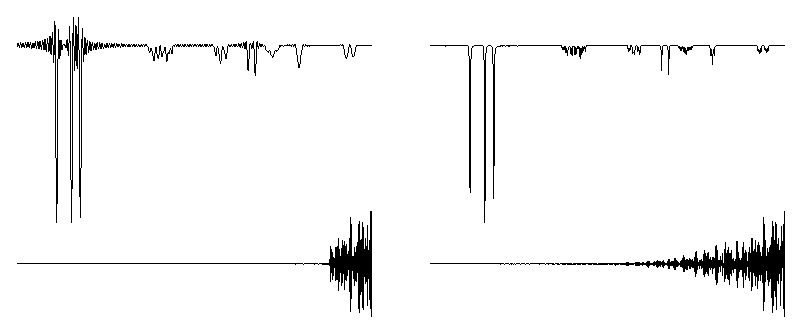
\epsfig{file=trunc.eps,width=5in,angle=180}
\end{center}
\caption[Effet de la troncature du \FID.]
{Effet de la troncature du \FID.
A gauche, le {\FID} non tronqué et le spectre correspondant.
A droite, le {\FID} tronqué et son spectre.}
\label{fig:trunc}
\end{figure}

Idéalement, le signal devrait être enregistré pendant un temps infini pour en 
recueillir l'intégralité. 
L'allongement du temps d'enregistrement entraîne une moindre 
efficacité de l'amélioration du rapport S/B par accumulation, une diminution du rapport 
S/B de chaque signal pris individuellement et enfin nécessite un volume de stockage du 
spectre important. 
Le temps d'enregistrement du signal, noté $\Delta t$, est déterminé par la 
largeur spectrale et par le nombre d'échantillons à enregistrer. Il se peut que l'amplitude 
du signal au temps $t = \Delta t$, proportionnelle à $\exp(-\Delta t/T_2^*)$
reste importante par rapport 
à l' amplitude initiale.
Le signal dont on calcule la TF est alors une fonction 
exponentielle décroissante tronquée et les raies du spectres ne seront plus de forme 
lorentzienne.

Déterminer la TF d'un signal $s(t)$ tronqué revient à calculer 
\begin{equation}
S(\Oms) = \int_0^{\Delta t} \exp(-i \Oms t). s(t) \, dt
\end{equation}
A titre d'exemple, si le signal est caractérisé par un $T_2^*$ infiniment long et une phase 
nulle, $s(t) = \exp(i \omzeros t)$ alors,
\begin{eqnarray}
S(\Oms) & = & \int_0^{\Delta t} \exp(-i t (\Oms - \omzeros)) d\Oms \\
& = & \frac{i}{\Oms - \omzeros} \left[ \exp(-i t(\Oms-\omzeros))\right]_0^{\Delta t} \\
& = & \frac{i}{\Oms - \omzeros} (\exp(i \Delta t (\Oms-\omzeros))-1)
\end{eqnarray}

Si on pose $u = \Delta t (\Oms -\omzeros)$ alors la partie réelle de 
$S(\Oms)$ vaut $\Delta t . \sin(u)/u$. 
Le spectre correspondant est tracé figure \ref{fig:sinc}, avec $\omzeros = 0$.
Cette fonction est centrée sur $\Oms = \omzeros$ et est significativement
différente d'une raie lorientzienne en absorption. 
La raie qui serait idéalement fine en l'absence de troncature 
a maintenant une largeur définie 
entre les points A et B, correspondant aux premières valeurs nulles de sin(u)/u, 
c'est-à-dire à $u = \pm\pi$. 
La largeur de la raie $\delta\Oms$ est alors telle que $\Delta t.\delta\Oms = 2 \pi$,
égale à la résolution numérique du spectre.
La raie est d'autant plus large que $\Delta t$ est court.

\begin{figure}[hbt]
\begin{center}
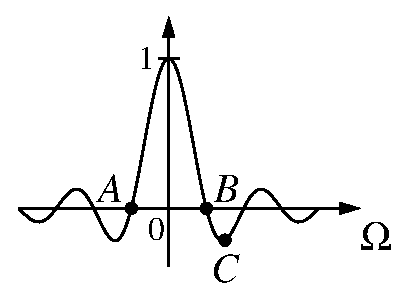
\epsfig{file=sinc.eps,width=3in}
\end{center}
\caption{Effet sur un spectre de la troncature du signal temporel.}
\label{fig:sinc}
\end{figure}

Qualitativement $\Delta t$ et $T_2^*$ 
jouent des rôles similaires puisque raccourcir le temps pendant lequel le signal a une 
intensité appréciable entraîne un élargissement des raies et une diminution de leur 
hauteur.
Toutefois, la relaxation n'introduit ni "pied" négatif dans le spectre ni de maxima 
secondaires. L'intensité de la première excursion négative (point C, figure \ref{fig:sinc}) 
est calculée pour $u = 3\pi/2$ et vaut $-2/3\pi = -0.212$, 
relativement à l'intensité du maximum principal. 
Des pics de faible intensité situés au voisinage du pic principal 
seront masqués par la distorsion de 
la ligne de base engendrée par la troncature.

Le cas analysé ici est un cas extrême, l'autre cas extrême est celui où $T_2^*$ est très 
inférieur à $\Delta t$. 
Au moment où cesse l'acquisition du signal il n'y a alors plus de signal 
mesurable (sauf du bruit) et la troncature n'a plus d'effet ni sur la largeur des raies ni sur 
leur forme. 
Dans les cas intermédiaires la troncature introduit un élargissement des raies 
et l'apparition de maxima secondaires positifs et négatifs, mais d'intensité relative plus 
faible qu'en l'absence de relaxation.

\section{L'apodisation}
Pour couper le pied (apodiser) négatif des raies issues d'un signal tronqué et restaurer leur 
forme lorentzienne, il suffit de multiplier $s(t)$ par une fonction exponentielle 
décroissante $\exp(-t/\tau)$ avec $\tau > 0$ (Figure \ref{fig:apodC}).
Le signal $s(t) = \exp(-t/T_2^*).\exp(i \omzeros t)$ devient 
$\exp(-t.(1/T_2^* + 1/\tau)).\exp(i \omzeros t)$. 
Tout se passe comme si $T_2^*$ avait été diminué, l'amortissement du 
signal étant caractérisé par un paramètre $\lambda$ tel que 
\begin{equation}
1/\lambda = 1/T_2^* + 1/\tau
\end{equation}
La largeur à mi-hauteur $\Delta\nu_{1/2}$ d'une raie lorentzienne est reliée à 
$\lambda$ par $\Delta\nu_{1/2} = 1/\pi\lambda$, 
l'apodisation par une fenêtre exponentielle décroissante $\exp(-t/\tau)$ élargit donc les raies 
de $1/\pi\lambda$ Hertz. 
Si $\tau$ est choisi suffisamment grand pour que le signal soit pratiquement 
nul à $t = \Delta t$, les raies du spectre ne présentent plus d'oscillations à leur base mais leur 
élargissement diminue la résolution du spectre.

L'apodisation n'est pas sans répercussion sur le rapport signal sur bruit du spectre.
Le bruit reste d'intensité constante de $t=0$ à $t=\Delta t$.
Puisque le signal issu de l'échantillon décroît au cours du temps, on peut
dire que le rapport signal sur bruit décroît aussi au cours de l'enregistrement.
Multiplier le signal par une exponentielle décroissante peut totalement
annuler le bruit lorsque $t$ est voisin de $\Delta t$.
Cette même opération atténue aussi le signal.
Il est possible de montrer que le rapport signal sur bruit est optimisé
lorsque qu'on apodise le signal avec $\tau = T_2^*$.

Lorsque le rapport signal sur bruit est important il est possible d'en tirer parti pour 
améliorer la résolution du spectre. 
Si le signal est multiplié par une fonction 
exponentielle croissante $\exp(t/\tau)$, ($\tau > 0$) 
la largeur à mi-hauteur des raies est diminuée de 1/$\pi\tau$ 
(en l'absence de troncature) et le rapport signal sur bruit diminue. 
En considérant que 
toutes les raies du spectre ont le même $T_2^*$, multiplier le signal par $\exp(t/T_2^*)$ 
compense complètement l'effet de la relaxation et les raies atteignent leur largeur 
minimale de l'ordre de $1/\Delta t$.
L'effet sur le rapport signal sur bruit peut alors être catastrophique.
Il faut donc multiplier à nouveau le signal temporel par une fonction
qui va atténuer fortement la fin
du signal tout en laissant le début le plus intact possible.
Cela se réalise par exemple avec une fonction gaussienne. 
Cette dernière va contribuer
bien entendu à élargir les raies, mais de manière contrôlable, tout en leur
donnant une forme assez complexe.
La transformation du signal résultante (Lorentz-Gauss) est pratiquement utilisée pour
faciliter la séparation de signaux de fréquences extrêmement voisines
(Figure \ref{fig:apodH}).
L'utilisateur doit rechercher un compromis entre les différentes
options qui lui permettent de modifier la résolution, la forme des raies, le
rapport sur bruit, et ceci en fonction du signal disponible et de la nature
des informations recherchées dans le spectre.

\section{Le zero filling}
La technique du "remplissage avec des zéros" contribue à l'amélioration de séparation 
entre raies de fréquences voisines, et consiste à faire suivre par des valeurs numériques 
nulles les valeurs du signal numérisé du signal avant transformée de Fourier. 
L'intérêt de cette manipulation est illustré figure \ref{fig:zerofill}, 
où le spectre $a$ est obtenu par TF d'un signal 
composé de 4094 valeurs complexes. 
Le signal en question est "allongé" à l'aide zéros 
jusqu'à obtenir un signal de 16384 valeurs complexe, les 12288 derniers étant nulles. 
Le spectre de droite, composé de 16384 points complexes présente des détails fins invisibles dans 
celui de gauche. Seule une petite région spectrale est représentée.

\begin{figure}[hbt]
\begin{center}
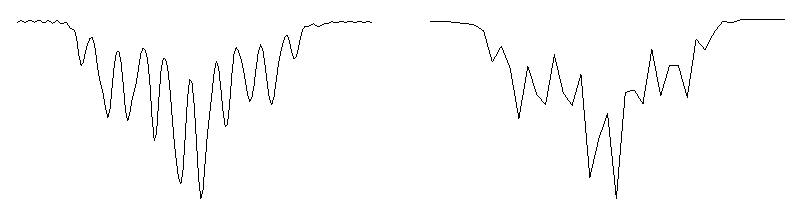
\epsfig{file=zerofill.eps,width=5in,angle=180}
\end{center}
\caption[Effet du zero-filling.]
{A gauche, spectre sans zero filling avant TF. A droite, le signal temporel a été allongé 4 fois.}
\label{fig:zerofill}
\end{figure}

Le zero filling a pour but d'augmenter artificiellement la résolution numérique
puisque la largeur spectrale ne change pas et que le nombre de points qui définit
la taille du spectre augmente (ce nombre est égal au nombre de valeurs du signal temporel).
Le zero filling fournit une interpolation de $S(\Oms)$ entre les valeurs issues d'une TF
sans zero filling.
Il est généralement admis que multiplier la taille du spectre par un facteur 2 apporte 
une amélioration utile, et qu'utiliser un facteur plus important n'apporte
pas d'amélioration sensible.

\section{Le programme de phases}
\label{sec:progphaseft}

Un spectre enregistré par la méthode impulsionnelle présentée dans ce chapitre peut présenter
des pics à des positions inattendues, et dont l'intensité
dépend de la qualité des dispositifs électroniques qui constituent
la chaîne d'acquisition du signal.
Un artefact exactement situé au milieu du 
spectre ($\Oms = 0$) est appelé pic axial et un artefact symétrique du pic réel par rapport au pic 
axial est appelé "fantôme de quadrature" ($\Oms = - \omzeros$)
pour une raison qui apparaîtra ci-après.
L'enregistrement de signaux successifs où les 
phases de l'impulsion et du récepteur sont modifiées entre chaque séquence excitation - 
détection permet l'élimination de ces artefacts. 
Le concept de programme de phase introduit ici sera 
réexaminé dans le cadre plus général des expériences multi--impulsionnelles.

L'analyse du programme de phase associé à une expérience de RMN
consiste à étudier comment varie le signal en 
fonction de la phase de l'impulsion (ou des impulsions) qui l'a créé. 
Dans l'expérience élémentaire "excitation - détection", 
il a été signalé qu'une augmentation de la phase de l'impulsion entraîne une 
augmentation identique de l'angle que fait la composante transversale
de l'aimantation avec l'axe $OX$.
En identifiant signal complexe et aimantation transversale dans le référentiel tournant,
augmenter de $\Delta \phi$ la phase de l'impulsion revient à 
multiplier $s(t)$ par $\exp(i.\Delta\phi)$. 
Ainsi si $\Delta\phi = \pi/2$, alors $s(t)$ devient $i.s(t)$. 

Un détecteur idéal est censé délivrer une tension nulle en l'absence de grandeur à 
mesurer. 
Dans la réalité, une tension continue, ou tension de décalage, 
est présente à la sortie du (ou des) détecteur(s). 
On notera $\epsilon$ cette tension et $s(t,\phi = 0)$ 
le "vrai" signal complexe en supposant 
que la phase $\phi$ de l'impulsion utilisée est nulle; 
le signal complexe mesuré est alors  $s(t, 0) + \epsilon = s'(t, 0)$. 
Le tableau \ref{tab:phasea} résume les valeurs du signal complexe 
mesuré en fonction de la phase de l'impulsion.

\begin{table}
\caption{Variation du signal en fonction de la phase de l'impulsion, 
effet d'une composante continue}
\label{tab:phasea}
\begin{center}
\begin{tabular}[hbt]{crcl}
\hline
Phase    &                     & $s(t)$ &          \\ \hline
$0$      &  $1.s(t,0) + \epsilon$ & = & $s'(t,0)$ \\
$\pi/2$  &  $i.s(t,0) + \epsilon$ & = & $s'(t,\pi/2)$ \\
$\pi$    &   $-s(t,0) + \epsilon$ & = & $s'(t,\pi)$ \\
$-\pi/2$ & $-i.s(t,0) + \epsilon$ & = & $s'(t,-\pi/2)$ \\
\hline
\end{tabular}
\end{center}  
\end{table}

Si on additionne $s'(t,0)$ et l'opposé de $s'(t,\pi)$ on constate l'annulation du terme 
d'erreur et l'addition constructive des signaux vrais : 
$s'(t,0) - s'(t,\pi) = 2.s(t,0)$. 
Ce résultat est général si on considère les signaux issus de deux impulsions de 
phases différent de $\pi$.

L'amplitude de la composante du signal ayant une fréquence nulle 
c'est-à-dire $S(\Oms = 0)$ est calculée par selon la définition de la TF : 
\begin{equation}
		S(0) = \intzp s(t).\exp(i.0.t) \, dt = \intzp s(t) \, dt
\end{equation}
qui correspond à la définition de la moyenne du signal. 
Superposer une composante $\epsilon$
continue au signal (de moyenne non nulle par définition) 
revient à modifier la valeur de 
$S(\Oms = 0)$ et donc à introduire dans le spectre un pic axial.
Utiliser $s'(t,0) - s'(t,\pi) = 2.s(t,0)$ au lieu
de $2(s(t,0)+\epsilon)$ permet donc d'éliminer le pic axial.

En supposant maintenant qu'il n'y a pas d'erreur de décalage mais une différence de gain 
d'amplification des signaux $s_x(t)$ et $s_y(t)$ issus des deux démodulateurs, le signal 
complexe effectivement enregistré lorsque la phase de l'impulsion est nulle s'écrit :
\begin{equation}
s'(t,0) = s_x(t,0).(1+\delta) + i.s_y(t,0).(1-\delta) 
\end{equation}
où $1+\delta$ et $1-\delta$ sont les gains relatifs des deux chaînes d'amplification. 
Ces gains sont en principe ajustés de façon à valoir 1 et 1 
mais des variations peuvent apparaître au cours du temps. 
L'effet de la dissymétrie entre les deux canaux de réception est mise en évidence 
en écrivant 
\begin{equation}
s'(t,0) = 1.(s_x(t,0) + i.s_y(t,0)) + \delta.(s_x(t,0) - i.s_y(t,0)) 
\end{equation}
si, pour simplifier, on omet le terme de relaxation et de phase du signal :
\begin{eqnarray}
s_x(t,0) &=& \cos(\omzeros t) \\
s_y(t,0) &=& \sin(\omzeros t)
\end{eqnarray}
alors :
\begin{equation}
		s'(t,0) = 1.\exp(i \omzeros t) + \delta.\exp(-i \omzeros t)
\end{equation}
la partie réelle de la TF de $s'(t,0)$ présente une raie 
d'intensité relative 1 à la pulsation $\omzeros$ et une autre raie, 
le "fantôme de quadrature", à la 
pulsation $-\omzeros$ et d'intensité relative $\delta$. 
On peut considérer que l'apparition de ce pic non 
voulu est lié à une incapacité du détecteur à distinguer parfaitement les fréquences 
positives des fréquences négatives lorsque les canaux de réception sont non 
symétriques. 
A l'extrême si un des canaux vient à ne plus fonctionner (gain nul), alors $\delta$ 
vaut 1 ou -1 : le pic attendu et son image de quadrature ont la même intensité, ce
qui correspond à une détection à une détection sur un seul canal et donc
à une indétermination du signe des fréquences.
 
Le tableau \ref{tab:phaseb} indique pour les diverses valeurs de phase $\phi$ de l'impulsion 
ce qu'est le signal enregistré $s'(t,\phi)$ en 
fonction de s(t,0) et de s*(t,0), avec 
\begin{eqnarray}
s(t,0) & = & s_x(t,0) + i.s_y(t,0) \\
s^*(t,0) & = & s_x(t,0) - i.s_y(t,0)
\end{eqnarray}

\begin{table}
\caption{Variation du signal en fonction de la phase de l'impulsion, 
effet d'une erreur de quadrature}
\label{tab:phaseb}
\begin{center}
\begin{tabular}[hbt]{cc}
\hline
$\phi$    &                      $s'(t,\phi)$           \\ \hline
$0$      &  $1.s(t,0)  + \delta.s^*(t,0)$ \\
$\pi/2$  &  $i.s(t,0) -i \delta.s^*(t,0)$ \\
$\pi$    &   $-s(t,0)  - \delta.s^*(t,0)$ \\
$-\pi/2$ & $-i.s(t,0) +i \delta.s^*(t,0)$ \\
\hline
\end{tabular}
\end{center}  
\end{table}


Ainsi augmenter $\phi$ de $\pi/2$ revient à multiplier le terme $s(t,\phi)$ par $i$ 
et le terme $s^*(t,\phi)$ par $-i$ : 
\begin{equation}
s'(t,\phi+\pi/2) = i . s(t,\phi) - \delta . i . s^*(t,\phi)
\end{equation}
Dans un cas plus général on aurait :
\begin{equation}
s'(t,\phi+\Delta \phi) = \exp(i \Delta \phi) . s(t,\phi) + 
\delta.\exp(i.-\Delta \phi) . s^*(t,\phi)
\end{equation}

Pour éliminer l'erreur de quadrature il suffit d'additionner 
$s'(t,0)$ et $-i . s'(t,\pi/2)$ :
\begin{eqnarray}
    s'(t,0)     & = & s(t,0) + \delta.s^*(t,0) \\
- i.s'(t,\pi/2) & = & s(t,0) - \delta.s^*(t,0)
\end{eqnarray}
et leur somme vaut $2.s(t,0)$ indépendamment de $\delta$.

On peut montrer que si le déphaseur du récepteur en quadrature (figure \ref{fig:spectrob})
effectue un déphasage différent de $\pi/2$, une erreur de quadrature se produit,
identique à celle qui résulte du déséquilibre entre les deux voies de réception.

Pour éliminer simultanément l'erreur de 
décalage et de quadrature ($\delta$ et $\epsilon$ non nuls) 
un calcul analogue à celui présenté ci-dessus indique qu'il faut calculer 
la somme :
\begin{equation}
	s'(t,0) - i.s'(t,\pi/2) - s'(t,\pi) + i.s'(t,-\pi/2)
\end{equation}
qui vaut $4.s(t,0)$ indépendamment de $\delta$ et de $\epsilon$. 
La notion de phase du récepteur permet de formaliser cette manipulation des signaux. 
Pour additionner de façon cohérente les signaux, 
c'est-à-dire pour renforcer les vrais signaux et annuler les 
imperfections il faut augmenter successivement la phase de l'impulsion par pas de $\pi/2$ et 
augmenter identiquement la phase du récepteur : 
augmenter la phase du récepteur 
de $\pi/2$ revient à multiplier le signal complexe par $\exp(-i.\pi/2) = -i$. 
Pour supprimer toute confusion due au vocabulaire il faudrait parler de 
"déphasage du signal après acquisition" plutôt que de phase du récepteur. 
La multiplication du signal par $-i$ compense la multiplication du 
signal complexe par $i$ introduite par l'augmentation  de $\pi/2$ de la phase de l'impulsion. 
Les signaux vrais sont les seuls à être multipliés par $i$, 
ce sont les seuls à être additionnés de façon constructive. 
Dans le cas de l'expérience impulsion -- détection traitée jusqu'ici, la 
relation entre phase du récepteur $\phi_R$ et phase de l'impulsion (ou phase de l'émetteur) 
est donc :
\begin{equation}
\Delta \phi_R = \Delta \phi.
\end{equation}

En utilisant les conventions introduites dans la table \ref{tab:phase},
le programme de phase qui vient d'être décrit se note :
\begin{eqnarray}
  \phi & = & (x, y, -x, -y) \\
\phi_R & = & (x, y, -x, -y)
\end{eqnarray}
l'élimination des pics indésirables n'étant réalisée qu'après addition de quatre signaux. 
La mise en {\oe}uvre pratique du changement de phase du récepteur se limite en fait à des 
additions ou à des soustractions de signaux réels : si $s'(t)$ est écrit comme $s_x'(t) + i.s_y'(t)$ 
les parties réelles et imaginaires des termes à sommer sont données dans le tableau \ref{tab:phasec}.

\begin{table}
\caption{Phase du récepteur}
\label{tab:phasec}
\begin{center}
\begin{tabular}[hbt]{ccc}
\hline
terme    &  partie réelle & partie imaginaire           \\ \hline
$s'(t)   $ & $s_x'(t) $ & $s_y'(t)$  \\
$-i.s'(t)$ & $s_y'(t) $ & $-s_x'(t)$ \\
$-s'(t)  $ & $-s_x'(t)$ & $-s_y'(t)$ \\
$i.s'(t) $ & $-s_y'(t)$ & $s_x'(t)$  \\
\hline
\end{tabular}
\end{center}  
\end{table}

Il suffit donc après chaque numérisation des signaux $s_x'(t)$ et $s_y'(t)$ de sommer les 
valeurs obtenues, munies du signe requis, vers la partie réelle ou vers la partie 
imaginaire du signal total, comme indiquée dans le tableau \ref{tab:phasec}.

La notion de programme de phase sera réexaminée au paragraphe \ref{sec:progphasedensite} 
dans le cadre du formalisme de la matrice densité.


\chapter{Diagrammes énergétiques}
\label{chap:diagram}

La démarche qui va être présentée dans le chapitre suivant,
intitulé "matrice densité", repose
sur l'acceptation par le lecteur d'un certain nombre de règles
très formelles, mais qui ont comme premier avantage de reproduire
les résultats connus pour les systèmes à un spin et fondés sur
la manipulation du vecteur aimantation macroscopique.
Leur second avantage est d'être applicables "les yeux fermés"
en étant sûr qu'au terme de calculs, parfois un peu lourds, certes,
des résultat reflétant la réalité du comportement de systèmes complexes
pourront être obtenus.
Cette "conception algébrique" de la RMN n'est pas nécessairement la préférée de tous,
et la "conception géométrique" du modèle de Bloch semble être pour certains
(le plus grand nombre ?) plus directement accessible car plus visuelle.

L'extension du modèle de Bloch aux systèmes à plusieurs spins relève 
de la connaissance préalable de leur diagramme énergétique.
Ce chapitre a pour but de présenter ces diagrammes
et d'introduire la notion de couplage scalaire, notion qui est centrale
pour l'étude des structures moléculaires par RMN.
La présentation du modèle de Bloch étendu sera faite ultérieurement,
après la présentation du formalisme de la matrice densité, et afin
de faire le lien entre les deux concepts. 

Les diagrammes énergétiques indiquent quels sont les états d'énergie accessibles
à un spin ou un système de spin plongés dans un champ magnétique $\bzerovecloc$.
L'absorption et l'émission d'énergie sous forme d'une onde électromagnétique
par le système s'effectue à des fréquences caractéristiques qui se déduisent
des valeurs des énergies possibles. 
Ces fréquences sont les mêmes que celles observées pour la précession de l'aimantation
dans le modèle de Bloch et son extension aux systèmes à plus de un spin.
Le diagramme énergétique d'un système de spins est donc utile à connaître,
même pour les inconditionnels de la démarche algébrique.
% Comme précédemment nous nous plaçons dans l'hypothèse des systèmes faiblement couplés
% et des impulsions parfaites.

\section{Systèmes à un spin}

Comme indiqué au début de cet ouvrage, la fréquence de résonance $\nu_I$ d'un noyau $I$,
de rapport gyromagnétique $\gamma_I$ soumis au champ local $\bzerovecloc (I)$ est :
\begin{equation}
\nu_I = \frac{\gi\bzerolocs (I)}{2\pi}
\end{equation}
sachant qu'ici $\nu_I$ représente une fréquence mesurable dans le référentiel
du laboratoire (et non pas dans le référentiel tournant).

La résonance du noyau $I$ est liée à l'existence de 2 niveaux énergétiques
qui avaient été notés $E_{\al}$ et $E_{\be}$ liés aux valeurs du nombre quantique $m_s(I)$
$+1/2$ et $-1/2$, respectivement.
En prenant comme référence (énergie 0)  l'énergie moyenne $(E_{\al} + E_{\be})/2 $,
on obtient $E_{\al} = -1/2.h\nu_I$ et $E_{\be} = +1/2.h\nu_I$, soit
\begin{equation}
E/h = -m_s(I) \nu_I
\end{equation}
ce qui aboutit au diagramme énergétique de la figure \ref{fig:diagrami}.
Les états liés à $m_s(I) = +1/2$ et $-1/2$ seront respectivement notés $\al$ et $\be$.

\begin{figure}[hbt]
\begin{center}
\begin{pspicture}(0,-1.5)(5,2.5)
\psline[linewidth=0.05]{->}(0.5,-1.5)(0.5,1.5)
\psline(0,0)(1,0)
\psline(1,0)(2,1)
\psline(1,0)(2,-1)
\psline[linewidth=1mm](2,1)(3,1)
\psline[linewidth=1mm](2,-1)(3,-1)
\psline{<->}(2.5,-1)(2.5,1)
\rput(0.5,2){$E/h$}
\rput(4.5,2){$m_s$}
\rput(3,0){$\nu_I$}
\rput(3.5,1){$\be$}
\rput(3.5,-1){$\al$}
\rput(4.5,1){$-1/2$}
\rput(4.5,-1){$+1/2$}
\end{pspicture}
\caption{\label{fig:diagrami}
\small Diagramme énergétique d'un spin 1/2 isolé $I$}
\end{center}
\end{figure}

Pour rappel, le chemin qui conduit du diagramme énergétique
vers la précession du vecteur $\aimvec$ hors équilibre à la
fréquence $\nu_I$ s'appuie sur le traitement par la mécanique classique du mouvement
de ce vecteur, traitement dont la légitimité est laissée à
l'appréciation (la crédulité ?) du lecteur qui ne maîtriserait pas
les aspects fondamentaux de la mécanique quantique.

En faisant une entorse aux principes exposés dans le préambule,
le raisonnement suivant présente le lien quantique entre niveaux énergétiques
et précession de Larmor.
Cela doit être considéré comme une digression...

Soient $\qal$ et $\qbe$ sont les fonctions propres de l'hamiltonien
\begin{equation}
H = -2\pi\nu_I \cdot I_z 
\end{equation}
avec respectivement comme valeurs propres $E_{\al}=-h\nu_I/2$ et $E_{\be}=+h\nu_I/2$.
L'état d'\emph{une seule} particule décrit par la fonction d'onde
\begin{equation}
\qpsi_0 = \frac{\qal + \qbe}{\sqrt{2}}
\end{equation}
est un état propre de $I_x$.
C'est-à-dire que si on dispose d'un grand nombre de particules
qui sont toutes à l'instant $t=0$ dans l'état $\qpsi_0$,
et si on mesure $\aimxs = \gamma_I I_x$ sur chaque particule,
alors on est \emph{certain} de trouver à chaque fois $1/2.\gamma_I\hbar$.
L'état $\qpsi_0$ va évoluer
au cours du temps, selon le résultat usuel, issu de l'intégration
de l'équation de Schrödinger dépendante du temps.
\begin{eqnarray}
\qal & \xrightarrow{H,t} & \exp(-iE_{\al}t/\hbar)\cdot \qal\\
\qbe & \xrightarrow{H,t} & \exp(-iE_{\be}t/\hbar)\cdot \qbe\\
\qpsi_0 & \xrightarrow{H,t} & \qpsi(t) \nonumber\\
& & = (\exp(-iE_{\al}t/\hbar) \cdot \qal + \exp(-iE_{\be}t/\hbar) \cdot \qbe)/\sqrt{2}
\end{eqnarray}
La probabilité $p_+(t)$ pour que la mesure de $\aimxs$ donne $+1/2.\gamma_I.\hbar$
est fournie par 
\begin{eqnarray}
p_+(t) & = & |\bpsi_0 \qpsi(t)|^2 \nonumber\\
& = & |\exp(-iE_{\al}t/\hbar) + \exp(-iE_{\be}t/\hbar)|^2/4 \nonumber\\
& = & (1 + \cos((E_{\be} -E_{\al})t/\hbar)/2 \label{eqn:interf}\\
& = & (1 + \cos(2\pi\nu_It))/2
\end{eqnarray}
Sachant que la valeur propre $-1/2.\gamma_I\hbar$ de $\aimxs$ est associée
à la fonction d'onde $(\qal - \qbe)/\sqrt{2}$,
un calcul identique au précédent conduit pour la probabilité 
$p_-(t)$ pour que la mesure de $\aimxs$ donne $-1/2.\gamma_I\hbar$
\begin{equation}
p_-(t)  =  (1 - \cos(2\pi\nu_It))/2
\end{equation}

La valeur moyenne de $\aimx$ au temps $t$, observable sur un grand nombre
de noyaux initialement tous dans l'état $\qpsi_0$ est donc
\begin{eqnarray}
<\aimxs(t)> & = & 1/2.\gamma_I\hbar(p_+(t) - p_-(t)) \nonumber\\
& = & 1/2.\gamma_I\hbar\cos(2\pi\nu_It)
\end{eqnarray}

Suivant la même procédure,
\begin{eqnarray}
<\aimys(t)> & = & -1/2.\gamma_I\hbar\sin(2\pi\nu_It)\\
<\aimzs(t)> & = & 0
\end{eqnarray} 
ce qui correspond une rotation à la fréquence $-\nu_I$ de $<\aimvec(t)>$,
en partant à $t=0$ d'une aimantation alignée sur l'axe $Ox$
du référentiel du laboratoire.

Ce raisonnement est très général et peut s'étendre à l'étude de l'action
du champ $\bunvec$.
Les principes la mécanique quantique se substituent parfaitement
à ceux de la mécanique classique sans introduire l'hypothèse supplémentaire
de la nécessaire validité de cette dernière dans le domaine macroscopique.
Le lecteur attentif aura remarqué que tout se joue dans l'équation
\ref{eqn:interf} où l'évolution sinusoïdale de $\aimxs(t)$ est liée à un
effet d'interférence quantique, tout à fait semblable
dans sa forme à une interférence optique.

Fin de la digression...

En résumé, c'est bien parce qu'il y a deux niveaux d'énergie $E_{\al}$
et $E_{\be}$ qu'il y a une précession de l'aimantation transversale à
la fréquence $(E_{\be} - E_{\al})/h$ et qu'il est donc intéressant
de tracer des diagrammes énergétiques.

\section{Systèmes à deux spins}
\subsection{Sans couplage scalaire}
Si deux systèmes sont réunis sans qu'ils interagissent entre eux,
leur énergie d'interaction avec l'extérieur est la somme
des énergies prises séparément.
On considère ici 2 noyaux $I$ et $S$ caractérisés par leur fréquence
de résonance $\nu_I$ et $\nu_S$.
L'énergie d'interaction $E$ s'exprime donc par
\begin{equation}
E/h = -m_s(I)\nu_I -m_s(S)\nu_S
\end{equation}
L'état quantique du système est défini par les valeurs de $m_s(I)$ et $m_s(S)$.
Sous forme symbolique, on note $\al\al$, $\al\be$, $\be\al$ et $\be\be$
les quatre états possibles de ce système composé de deux spins $1/2$,
le premier signe étant relatif à $I$ et le second à $S$.

Toutes les transitions énergétiques envisageables ne sont cependant pas
réalisables par émission ou absorption d'une onde électromagnétique.
Pour savoir quelles sont les transitions autorisées il faut d'abord
définir le nombre quantique total :
\begin{equation}
m_s = m_s(I) + m_s(S)
\end{equation}
pour définir la règle de sélection :
\begin{equation}
|\Delta m_s| = 1
\end{equation}
qui se justifie à la fois par la loi de conservation du moment cinétique
et l'attribution du spin 1 au photon, la particule
associée au rayonnement électromagnétique.
Pour cette raison, les transitions observables sont aussi appelées
transitions "à $\pm 1$ quanta" ou "à simple quanta".

Il en résulte quatre transitions possibles, pour lesquelles
soit $\Delta m_s(I) = 1$ et $\Delta m_s(S) = 0$,
soit $\Delta m_s(S) = 0$ et $\Delta m_s(S) = 1$.
Les deux premières sont dites "transitions de $I$" et
les secondes "transitions de $S$", comme
indiqué sur la figure \ref{fig:diagramis}.

\begin{figure}[hbt]
\begin{center}
\begin{pspicture}(0,-3.5)(14,4)
\psline[linewidth=0.05]{->}(0.5,-3.5)(0.5,3.5)
\rput(0.5,4){$E/h$}
\psline(0,0)(1,0)
\psline(1,0)(1.5,2)
\psline(1,0)(1.5,-2)
\psline(1.5,2)(2.5,2)
\psline(1.5,-2)(2.5,-2)
\psline{<->}(2,-2)(2,2)
\rput(2.5,0){$\nu_I$}
\psline(2.5,2)(3,3)
\psline(2.5,2)(3,1)
\psline(2.5,-2)(3,-1)
\psline(2.5,-2)(3,-3)
\psline[linewidth=1mm](3,3)(4,3)
\psline[linewidth=1mm](3,1)(4,1)
\psline{<->}(3.5,1.05)(3.5,2.95)
\rput(4,2){$\nu_S$}
\psline[linewidth=1mm](3,-3)(4,-3)
\psline[linewidth=1mm](3,-1)(4,-1)
\psline{<->}(3.5,-1.05)(3.5,-2.95)
\rput(4,-2){$\nu_S$}
\rput(4.5,0){
 \rput(0,3){$\be\be$}
 \rput(0,1){$\be\al$}
 \rput(0,-1){$\al\be$}
 \rput(0,-3){$\al\al$}
}
\rput(5.5,0){
 \rput(0,4){$m_s(I)$}
 \rput(0,3){$-1/2$}
 \rput(0,1){$-1/2$}
 \rput(0,-1){$+1/2$}
 \rput(0,-3){$+1/2$}
}
\rput(7,0){
 \rput(0,4){$m_s(S)$}
 \rput(0,3){$-1/2$}
 \rput(0,1){$+1/2$}
 \rput(0,-1){$-1/2$}
 \rput(0,-3){$+1/2$}
}
\rput(8.5,0){
 \rput(0,4){$m_s$}
 \rput(0,3){$-1$}
 \rput(0,1){$0$}
 \rput(0,-1){$0$}
 \rput(0,-3){$+1$}
}
\rput(11.5,0){
 \psline[linewidth=1mm](-2.5,1)(-1.5,1)
 \rput(-1,1){$\be\al$}
 \psline[linewidth=1mm](-0.5,3)(0.5,3)
 \rput(0,3.5){$\be\be$}
 \psline[linewidth=1mm](0.5,-3)(-0.5,-3)
 \rput(0,-3.5){$\al\al$}
 \psline[linewidth=1mm](2.5,-1)(1.5,-1)
 \rput(1,-1){$\al\be$}
 \psline{<->}(-2,1.05)(0,2.95)
 \rput(-1.5,2.5){$\nu_S$}
 \psline{<->}(-2,0.95)(0,-2.95)
 \rput(-1.5,-1.5){$\nu_I$}
 \psline{<->}(2,-1.05)(0,-2.95)
 \rput(1.5,-2.5){$\nu_S$}
 \psline{<->}(2,-0.95)(0,2.95)
 \rput(1.5,1.5){$\nu_I$}
}
\end{pspicture}
 \caption{\label{fig:diagramis}
 Diagramme énergétique d'un système $IS$ de 2 spins non couplés
 }
\end{center}
\end{figure}

Les fréquences de résonance associées $\nu_I$ et $\nu_S$ sont données par
\begin{eqnarray}
h \nu_I & = & E_{\be\be} - E_{\al\be} = E_{\be\al} - E_{\al\al}\\
h \nu_S & = & E_{\be\be} - E_{\be\al} = E_{\al\be} - E_{\al\al}
\end{eqnarray}

Les noyaux $I$ et $S$ n'ont aucune interaction et le spectre observable
ne fera intervenir que leurs propres fréquences.

Les transitions (une dans chaque sens) entre les états énergétiques 
$\al\al$ et $\be\be$ correspondent à $\Delta m_s = \pm 2$ et sont
appelées transitions "à double quanta" ;
celles entre $\al\be$ et $\be\al$ sont des transitions "à 0 quanta".

\subsection{Avec couplage scalaire}

Deux noyaux $I$ et $S$ de même nature (système $IS$ homonucléaire) ou de nature 
différentes (système $IS$ hétéronucléaire) peuvent interagir entre eux par couplage 
scalaire (appelé ainsi parce qu'il s'exprime sous la forme d'un produit scalaire d'opérateurs...).
Cette interaction a pour médiateurs les orbitales moléculaires et les spins électroniques.
Elle est caractérisée à son intensité $J$, appelée constante de couplage
et mesurée en Hertz.

Le couplage est fort si $J$ est comparable ou plus grand 
que la différence des fréquences de résonance des noyaux $I$ et $S$. 
Cela n'est jamais le cas 
pour les systèmes hétéronucléaires et peu fréquent dans les systèmes homonucléaires, 
surtout à des valeurs élevées du champ magnétique $\bzeros$.
Pour les systèmes faiblement couplés, l'expression de l'énergie
du système des deux spins $I$ et $S$ comporte un terme supplémentaire
lié à l'existence du couplage :
\begin{equation}
E/h = -m_s(I)\nu_I -m_s(S)\nu_S + Jm_s(I)m_s(S)
\end{equation}

Les règles de sélection restant valides (par ce que les couplages sont faibles),
quatre transitions sont observables.
Leurs fréquences sont maintenant toutes différentes et données par :
\begin{eqnarray}
\nu_1 & = & (E_{\be\al} - E_{\al\al})/h = \nu_I - J/2 \\
\nu_2 & = & (E_{\be\be} - E_{\al\be})/h = \nu_I + J/2 \\
\nu_3 & = & (E_{\al\be} - E_{\al\al})/h = \nu_S - J/2 \\
\nu_4 & = & (E_{\be\be} - E_{\be\al})/h = \nu_S + J/2
\end{eqnarray}
Comme indiqué dans la figure \ref{fig:diagramisj}.
Les deux premières fréquences sont liées aux transitions à simple ($\pm 1$) quanta
du noyau $I$ et les deux dernières aux transitions à simple quanta
de $S$.
Ce qui différence les fréquences des deux transitions de $I$ (ou de $S$)
réside simplement dans le fait que l'état du spin $S$ (ou de $I$)
est soit $\al$ soit $\be$.
Dans le premier cas la fréquence de la transition est diminuée de $J/2$,
dans le second cas elle est augmentée de $J/2$.
Une transition d'un noyau est donc pleinement définie à partir de la
donnée de l'état de l'autre noyau du système, ou des autres noyaux s'il
y en a plus que deux dans le système.

\begin{figure}[hbt]
\begin{center}
\begin{pspicture}(0,-3.5)(14,4)
\psline[linewidth=0.05]{->}(0.5,-3.5)(0.5,3.5)
\rput(0.5,4){$E/h$}
\psline(0,0)(1,0)
\psline(1,0)(1.5,2)
\psline(1,0)(1.5,-2)
\psline(1.5,2)(2.5,2)
\psline(1.5,-2)(2.5,-2)
\psline{<->}(2,-2)(2,2)
\rput(2.5,0){$\nu_I$}
\psline(2.5,2)(3,3)
\psline(2.5,2)(3,1)
\psline(2.5,-2)(3,-1)
\psline(2.5,-2)(3,-3)
\psline(3,3)(4,3)
\psline(3,1)(4,1)
\psline{<->}(3.5,1)(3.5,3)
\rput(4,2){$\nu_S$}
\psline(3,-3)(4,-3)
\psline(3,-1)(4,-1)
\psline{<->}(3.5,-1)(3.5,-3)
\rput(4,-2){$\nu_S$}
\psline(4,3)(4.5,3.5)
\psline(4,1)(4.5,0.5)
\psline(4,-1)(4.5,-1.5)
\psline(4,-3)(4.5,-2.5)
\psline[linewidth=1mm](4.5,3.5)(5.5,3.5)
\psline[linewidth=1mm](4.5,0.5)(5.5,0.5)
\psline[linewidth=1mm](4.5,-2.5)(5.5,-2.5)
\psline[linewidth=1mm](4.5,-1.5)(5.5,-1.5)
\rput(5,0){
 \rput(0,3){$\be\be$}
 \rput(0,1){$\be\al$}
 \rput(0,-1){$\al\be$}
 \rput(0,-3){$\al\al$}
}
\rput(6,0){
 \psline{->}(0,3)(0,3.5)
 \psline{->}(0,1)(0,0.5)
 \psline{->}(0,-1)(0,-1.5)
 \psline{->}(0,-3)(0,-2.5)
}
\rput(7,0){
 \rput(0,4){$Jm_s(I)m_s(S)$}
 \rput(0,3.25){$+J/4$}
 \rput(0,0.75){$-J/4$}
 \rput(0,-1.25){$-J/4$}
 \rput(0,-2.75){$+J/4$}
}
\rput(11.5,0){
 \psline[linewidth=1mm](-2.5,0.5)(-1.5,0.5)
 \rput(-1,0.5){$\be\al$}
 \psline[linewidth=1mm](-0.5,3.5)(0.5,3.5)
 \rput(0,4){$\be\be$}
 \psline[linewidth=1mm](0.5,-2.5)(-0.5,-2.5)
 \rput(0,-3){$\al\al$}
 \psline[linewidth=1mm](2.5,-1.5)(1.5,-1.5)
 \rput(1,-1.5){$\al\be$}
 \psline{<->}(-2,0.55)(0,3.45)
 \rput(-2,2){$\nu_S+J/2$}
 \psline{<->}(-2,0.45)(0,-2.45)
 \rput(-2,-1){$\nu_I-J/2$}
 \psline{<->}(2,-1.55)(0,-2.45)
 \rput(2,-2.25){$\nu_S-J/2$}
 \psline{<->}(2,-1.45)(0,3.45)
 \rput(2,1.5){$\nu_I+J/2$}
}
\end{pspicture}
 \caption{\label{fig:diagramisj}
 Diagramme énergétique d'un système $IS$ de 2 spins faiblement couplés.
 }
\end{center}
\end{figure}

La constante de couplage $J$ est expérimentalement accessible en remarquant
que :
\begin{equation}
J = \nu_2 - \nu_1 = \nu_4 - \nu_3 
\end{equation}

Remarquons enfin que les fréquences des transitions à double (DQ) et à zéro (ZQ) quanta
ne dépendent pas de la valeur de $J$ :
\begin{eqnarray}
\nu_{\mbox{\scriptsize{DQ}}} & = & (E_{\be\be} - E_{\al\al})/h = \nu_I + \nu_S \\
\nu_{\mbox{\scriptsize{ZQ}}} & = & (E_{\be\al} - E_{\al\be})/h = \nu_I - \nu_S
\end{eqnarray}

\section{Systèmes à trois spins}
L'énergie d'un système de trois spins faiblement couplés $ISL$ est donnée par :
\begin{eqnarray}
E/h & = & -m_s(I) \nu_I -m_s(S) \nu_S -m_s(L) \nu_L \\
& & \quad + J_{IS} m_s(I) m_s(S) + J_{IL} m_s(I) m_s(L) + J_{SL} m_s(S) m_s(L)
\end{eqnarray}
chacune des constantes de couplage étant faible devant la différence
des fréquences de résonance des noyaux dont elle décrit le couplage.
Un système de trois spins possède donc 8 niveaux énergétiques possibles.
Les transitions autorisées sont celles pour lesquelles
\begin{equation}
|\Delta m_s| = 1
\end{equation}
avec
\begin{equation}
m_s = m_s(I) + m_s(S) + m_s(L)
\end{equation}
où, à nouveau, $m_s$ est le nombre quantique associé à la projection sur
un axe du moment cinétique total du système.

La figure \ref{fig:diagramisl} représente symboliquement les 8 niveaux 
et les douze transitions observables dans un système $ISL$ faiblement couplé.

\begin{figure}[hbt]
\begin{center}
\begin{pspicture}(-4,-3.5)(4,3.5)
\psline[linewidth=1mm](-0.5,3)(0.5,3)
\psline[linewidth=1mm](-3.5,1)(-2.5,1)
\psline[linewidth=1mm](-0.5,1)(0.5,1)
\psline[linewidth=1mm](2.5,1)(3.5,1)
\psline[linewidth=1mm](-0.5,-3)(0.5,-3)
\psline[linewidth=1mm](-3.5,-1)(-2.5,-1)
\psline[linewidth=1mm](-0.5,-1)(0.5,-1)
\psline[linewidth=1mm](2.5,-1)(3.5,-1)
\rput(0,3.5){$\be\be\be$}
\rput(-4,1.5){$\al\be\be$}
\rput(-0.6,1.5){$\be\al\be$}
\rput(4,1.5){$\be\be\al$}
\rput(0,-3.5){$\al\al\al$}
\rput(4,-1.5){$\be\al\al$}
\rput(0.6,-1.5){$\al\be\al$}
\rput(-4,-1.5){$\al\al\be$}
\psline{<->}(0,2.95)(-3,1.05)
\psline{<->}(0,2.95)(0,1.05)
\psline{<->}(0,2.95)(3,1.05)
\psline{<->}(-3,0.95)(-3,-0.95)
\psline{<->}(-3,0.95)(0,-0.95)
\psline{<->}(-3,-0.95)(0,0.95)
\psline{<->}(0,-2.95)(3,-1.05)
\psline{<->}(0,-2.95)(0,-1.05)
\psline{<->}(0,-2.95)(-3,-1.05)
\psline{<->}(3,-0.95)(3,0.95)
\psline{<->}(3,-0.95)(0,0.95)
\psline{<->}(3,0.95)(0,-0.95)
\end{pspicture}
 \caption{\label{fig:diagramisl}
 Diagramme énergétique d'un système de 3 spins $ISL$.
 }
\end{center}
\end{figure}

Ainsi, par exemple, la transition $\be\al\al \rightarrow \be\be\al$ est une transition
du noyau $S$ qui s'opère avec $I$ dans l'état $\be$ et $L$ dans l'état $\al$.
Sa fréquence est la somme de trois termes : $\nu_S$ parce que c'est une transition
de $S$, $+J_{IS}/2$ car $I$ est dans l'état $\be$ et $-J_{SL}/2$ car $L$ est dans
l'état $\alpha$, soit au total 
\begin{equation}
\nu(\be\al\al \rightarrow \be\be\al) = \nu_S + J_{IS}/2 - J_{SL}/2
\end{equation}

La transition $\al\al\be \rightarrow \be\be\al$ satisfait à la condition
$|\Delta m_s| = 1$ bien que sa probabilité d'observation soit nulle.
Il y a au total trois transitions de ce genre qui sont inobservables.
Dans les systèmes fortement couplés $ABC$ il est possible d'observer
jusqu'à 15 (12 + 3) transitions.

\section{Diagramme énergétique et population des états}

Les différents niveaux énergétiques d'un système en équilibre thermodynamique
sont peuplés par les noyaux en fonction de la distribution de Boltzman.
Comme il a déjà été souligné, les différences d'énergie entre niveaux sont
très faibles par rapport $kT$ dans les conditions usuelles de température,
et donc les noyaux se répartissent à peu près équitablement
entre les niveaux possibles. 
Cet "à peu près" fait toute la différence puisque
l'intensité du signal observable est proportionnelle aux différences de population,
comme cela a été étudié en détail pour un spin isolé.

Un système de $n$ spins 1/2 possède $2^n$ niveaux énergétiques puisque chaque spin
peut être soit dans l'état $\al$ soit dans l'état $\be$.
Chaque niveau d'énergie $E_i (1 \le i \le 2^n)$ d'un ensemble de $P$ systèmes
de spins identiques est peuplé par $p_i$ noyaux avec
\begin{eqnarray}
\sum_i^{2^n} p_i & = & P \\
p_i & = & Z \exp(-E_i/kT) = Z(1 - E_i/kT)
\end{eqnarray}
dans l'hypothèse où $E_i \ll kT$.
$Z$ est un facteur de proportionnalité qui est déterminé par
\begin{eqnarray}
P & = & \sum_i^{2^n} (Z - ZE_i/kT) \\
& = & 2^n Z - Z/kT \sum_i^{2^n} E_i \\
& = & 2^n Z
\end{eqnarray}
sachant que la somme des énergies de tous les niveaux est nulle (il
suffit de faire l'addition pour s'en rendre compte).
Deux états indexés $i$ et $j$ d'énergie $E_i$ et $E_j$ auront comme population
$p_i = Z(1-E_i/kT)$ et $p_j = Z(1-E_j/kT)$ soit une différence de population
\begin{equation}
\label{eqn:diffpop}
p_i - p_j = -P/2^n.(E_i - E_j)/kT
\end{equation}
proportionnelle à leur différence d'énergie.
Il est utile de signaler qu'étant donné que les constantes de couplage
scalaire sont au plus de quelques centaines de Hz (sauf cas exceptionnels)
et que les fréquences de résonance sont de l'ordre de quelques dizaines
ou quelques centaines de MHz, les populations ne sont pas affectées par
l'intensité des couplages.

En considérant par exemple le noyau $I$ d'un système $ISL$ ($n$ = 3),
les différences de population $p_{\al i j} -p_{\be i j}$, avec $i$ et $j$
valant $\al$ ou $\be$, sont toutes égales :
\begin{eqnarray}
p_{\al i j} -p_{\be i j} & = & P/8.h\nu_I/kT \\
& = & P/8.\gamma_I.\hbar \bzeros/kT
\end{eqnarray}
sachant que les écarts énergétiques apportés par les déplacements chimiques
($E/h$ est de l'ordre de quelques dizaines de kHz tout au plus)
sont aussi trop faibles pour perturber notablement les populations.
Les différences de population considérées ici sont d'une grande importance pratique
car elles correspondent à des états pour lesquels des transitions sont
observables et car les intensités de ces transitions sont proportionnelles
aux différences de population correspondantes.

Il est possible de définir la différence de population $\Delta P(I)$ du noyau
$I$ comme étant la somme des différences de population correspondant
aux quatre états possibles des spins $S$ et $L$ :
\begin{eqnarray}
\Delta P(I) & = & (p_{\al \al \al} -p_{\be \al \al}) + (p_{\al \al \be} -p_{\be \al \be})
\nonumber\\
& & \quad + (p_{\al \be \al} -p_{\be \be \al}) + (p_{\al \be \be} -p_{\be \be \be}) \\
& = & P.\gamma_I.\hbar B_0/2kT
\end{eqnarray}
Cette valeur est indépendante du nombre de spins dans le système : le facteur 2
au dénominateur provient du rapport $2^n/2^{n-1} = 2$, sachant que $2^n$ provient
de l'équation \ref{eqn:diffpop} et que $2^{n-1}$ est le nombre d'états possibles
une fois que l'état d'un noyau a été fixé.

Le concept de différence de population pour un noyau est utile pour définir
la contribution de chaque noyau $I$ au vecteur aimantation macroscopique
global de l'échantillon $\aimzeros$ dans sa situation d'équilibre.
Ainsi,
\begin{eqnarray}
\aimzerozs(I) & = & \Delta P(I) . \gamma(I)\hbar/2 \\
& = & P.\gamma(I)^2.\hbar^2 B_0/4kT
\end{eqnarray}
le résultat établi pour un spin 1/2 isolé restant valable pour un spin 1/2
appartenant à un système de spins couplés.
Il faut toutefois noter que dans le cas d'un système à $n$ spins, 
la contribution de chaque noyau à $\aimzerovec$
résulte de la sous-contribution de $2^{n-1}$ vecteurs aimantation macroscopique
identiques (vecteurs élémentaires), 
chacun étant associé à une énergie d'une transition observable,
c'est-à-dire à une fréquence de résonance mesurable.

La mise hors équilibre de l'aimantation de l'échantillon par création
d'aimantation transversale est le moyen de mettre en évidence
les transitions entre niveaux énergétiques.
Chaque vecteur élémentaire décrit ensuite le mouvement de précession de Larmor
à la fréquence égale à la fréquence de la transition qui lui correspond.
Tout ceci constitue la base du modèle vectoriel de la RMN, généralisé aux systèmes
faiblement couplés. Le modèle vectoriel sera étudié plus en détail, après avoir
exposé la description de la RMN à l'aide du concept de matrice densité.

\chapter[La Matrice Densité]{La Matrice Densité}
\label{chap:densite}

\section{Position du problème}
La description physique du phénomène de résonance magnétique nucléaire
peut s'effectuer à (au moins) trois niveaux, faisant appel aux diagrammes énergétiques,
au vecteur d'aimantation macroscopique (le modèle de Bloch) et au formalisme
de la matrice densité.
Le modèle de Bloch, présenté précédemment, donne une image réaliste de 
l'évolution d'un système de noyaux isolés magnétiquement les uns des autres. 
Ce modèle peut être étendu pour y inclure l'action
des couplages scalaires. 
Il a ici semblé utile d'introduire le formalisme de la matrice densité à un 
niveau très élémentaire plutôt que de continuer avec le modèle de Bloch,
afin de faciliter l'étude d'expériences complexes 
faisant appel, par exemple, aux transitions à multiple quanta et
de justifier simplement la structure du programme de phase associé à une séquence 
multi-impulsionnelle. 

S'il est relativement aisé de comprendre comment utiliser
un diagramme énergétique ou une représentation vectorielle,
la caractérisation d'un système physique par une matrice
n'est pas usuellement ressentie comme intuitive.
La matrice densité possède une définition parfaitement rigoureuse dans 
le cadre du formalisme de la mécanique quantique.
Ce dernier n'est pas immédiatement accessible au non-initié,
et aurait même une action fortement répulsive.
Il n'est d'autre part pas évident de justifier 
par la seule compréhension de la RMN
la nécessité de l'assimilation préalable d'un volumineux
corpus de connaissances générales en mécanique quantique.
L'expérience montre qu'il est possible d'utiliser un nombre minimal
de définitions et de règles, sans démonstration, pour parvenir à une
description de la RMN utilisant la matrice densité et
qui soit opérationnelle dans la plus part des situations usuelles.
Le lecteur curieux et séduit par la puissance de cette approche n'en sera que
plus motivé pour aborder l'apprentissage des fondements de la mécanique quantique,
et découvrir l'origine des règles qu'il aura utilisées de prime
abord en toute innocence.
La matrice densité sera donc par la suite un objet dont il sera question
sans qu'une définition formelle ne lui ait été préalablement donnée.
Cette démarche non conventionnelle, surtout au pays de Descartes,
est cependant d'un intérêt certain, même
si elle peut dérouter.

Le concept de matrice densité est utilisé par les physiciens pour décrire le 
comportement d'un ensemble de particules qui ne présentent pas toutes le même état. 
Un système composé d'une particule ou d'un ensemble de particules de 
même état (cette situation est désignée sous l'appellation "cas pur") est 
parfaitement décrit par une fonction d'onde, fonction dont on sait tirer les probabilité de 
mesures de différentes grandeurs observables (position, quantité de mouvement, 
moment cinétique, énergie mécanique totale...) et dont l'évolution dans le temps est 
prévisible grâce à l'équation de Schrödinger.
Un système constitués de $P$ particules de spin 1/2, dont $p_{\al}$ et $p_{\be}$ sont 
dans l'état $m_s = +1/2$ et $m_s = -1/2$ ne peut être correctement 
décrit par une fonction d'onde.
Cette situation (appelée cas impur, ou mélange statistique) est celle
présentée par échantillon en équilibre (au sens thermodynamique du terme) dans un 
champ magnétique, au début de toute expérience de RMN. 
Dans un cas pur, matrice densité et fonction d'onde sont deux représentations 
équivalentes du système considéré. 
Il est possible de déduire de la matrice densité tous les résultats des 
mesures voulues et de déterminer leur évolution au cours du temps. 
Un mélange statistique est la réunion de sous-systèmes purs et 
la matrice densité associée à ce mélange est alors la moyenne 
des matrices densité des sous-systèmes dont il est composé, 
moyenne pondérée par les populations.
La matrice densité dans un cas pur ou dans un cas impur est utilisée de la même manière et 
constitue donc une sorte de généralisation de la fonction d'onde.

Connaissant la matrice densité d'un échantillon dans son état initial et les différents 
événements qui vont survenir (impulsions de radiofréquence entrecoupées de délais 
d'évolution), il sera possible de déterminer la matrice densité à chaque instant de 
l'acquisition du signal de précession libre. 
La grandeur observable, qui est la 
composante horizontale du moment magnétique de l'échantillon, sera déduite de la 
matrice densité.

Une matrice, d'une manière générale, est la représentation d'une transformation (ou opérateur)
linéaire qui transforme un élément d'un espace vectoriel en un autre élément
d'un espace vectoriel (le même ou un autre), ces espaces étant définis sur un même corps
(le corps des nombres complexes, en ce qui concerne ce qui va suivre).
Si le vecteur d'origine appartient à un espace de dimension $m$ et celui
d'arrivée à un espace de dimension $n$,
la matrice qui représente la transformation est un tableau de nombres complexes
possédant $n$ lignes et $m$ colonnes.

Pour situer le degré de complexité des calculs à effectuer, il faut savoir qu'analyser un 
système de $n$ spins couplés nécessite la manipulation de matrices à $2^n$ lignes et $2^n$ 
colonnes! 
De tels calculs sont très largement simplifiés si la matrice densité est 
exprimée comme une somme de matrices, multiples de matrices de base judicieusement 
choisies. 
La taille $n$ du système de spins étant fixée, il y a autant
de matrices de base que d'éléments dans la matrice soit $4^n$. 
Les matrices de base sont désignées sous forme symbolique facile à mémoriser. 
Bien qu'il existe une infinité d'ensembles possibles de matrices de base,
les "produits d'opérateurs cartésiens" seront préférentiellement choisis comme base.
Une base (c'est-à-dire un ensemble de matrices de base) étant choisie, 
des règles de calcul permettent de prévoir l'évolution de la 
matrice densité pendant les évènements qui constituent une séquence d'impulsions.
Chaque événement, impulsion ou délai, est associé à une opération linéaire
qui transforme la matrice densité du système avant l'événement en la matrice densité
après l'événement.
Une telle transformation, qui associe une matrice à une autre matrice, 
est appelée "super--opérateur".

Les règles d'évolution et d'utilisation de la matrice densité seront d'abord
introduites à propos des systèmes à un et deux spins.
D'autres règles permettront de calculer les grandeurs observables
$\aimxs$ et $\aimys$, projections de l'aimantation sur les axes
transversaux du référentiel tournant.
La généralisation de ces règles aux systèmes plus 
complexes procède des mêmes méthodes de calcul. 

\section{Le système à un spin}
\subsection{Les opérateurs cartésiens}
Un système à un spin (pour lequel on peut espérer retrouver les résultats du modèle de 
Bloch) est formé d'un noyau que l'on note $I$.
Les quatre matrices de base qui constituent la base d'opérateurs cartésiens
seront désignées par $E/2$, $I_x$, $I_y$ et $I_z$.
D'une manière générale, la matrice densité du système de spins considéré peut toujours s'écrire
\begin{equation}
\sigma = a \cdot E/2 + b \cdot I_x + c \cdot I_y + d \cdot I_z
\end{equation}
où $a$, $b$, $c$ et $d$ sont des nombres réels.
Les matrices $I_x$, $I_y$ et $I_z$ sont aussi appelées les matrices de Pauli.
La matrice identité $E$ intervient sous forme de E/2 pour des raisons
d'homogénéité des propriétés des matrices de base.
Les quatre matrices de base permettent de définir tout état du système de spins.
L'ensemble de tous les états possible constitue ce qui est appelé l'\emph{espace des états}.

\subsection{État initial}
La matrice densité, notée $\sigma$, d'un ensemble de $P$ noyaux plongé dans un champ magnétique, 
et ayant atteint une situation d'équilibre est :
\begin{equation}
\sigma_0 = P \cdot E/2 + \Delta P \cdot I_z
\end{equation}
où $\Delta P$ est la différence des populations initiales $p_{\al} - p_{\be}$ 
(voir p. \pageref{page:population}). 
La matrice $E$ étant la matrice identité, sa transformation par un opérateur linéaire
donnera toujours la matrice identité.
Sa contribution à $\sigma$ n'évolue pas au cours du temps.
Pour cette raison le terme proportionnel à $E/2$ sera toujours omis 
dans la suite des calculs. 
Ainsi,
\begin{equation}
\sigma_0 = \Delta P \cdot Iz
\end{equation}
Le coefficient multiplicatif $\Delta P$ se retrouvera tout au long du calcul de l'évolution
de la matrice densité du système, par linéarité des transformations qu'elle subit. 
Par souci de clarté, ce facteur sera aussi omis dans les calculs. 
Néanmoins, si on veut comparer différentes techniques du point de vue quantitatif, 
il est nécessaire de se souvenir de l'existence de ce facteur.
L'état initial du système sera donc décrit par :
\begin{equation}
\sigma_0 = I_z
\end{equation}

\subsection{Évènements}
\label{sec:evenements}
L'effet d'une impulsion ou de l'évolution libre du système pendant un délai
est calculé par action d'un super-opérateur sur la matrice densité. 
Par linéarité, si une matrice $\sigma$ est la somme de deux matrices
$I_a$ et $I_b$ ($a$ ou $b$ = $x$, $y$, ou $z$) multipliées par les 
coefficients $a$ et $b$ :
\begin{equation}
\sigma =  a \cdot I_a + b \cdot I_b
\end{equation}
et si $\hat{O}$ est le super-opérateur associé à un événement 
(impulsion ou délai) alors $\sigma'$, transformée de $\sigma$ par $\hat{O}$, 
se déduit des transformées de $I_a$ et $I_b$ par $\hat{O}$ :
\begin{equation}
\sigma' = \hat{O}(\sigma) = a \cdot \hat{O}(I_a) + b \cdot \hat{O}(I_b)
\end{equation}
Il suffit donc de connaître le résultat de la transformation des matrices de base pour 
calculer le résultat de la transformation de toute matrice.

Tout événement est caractérisé par l'\emph{interaction} entre les spins et l'extérieur
ainsi que par sa \emph{durée}.
Une interaction est \emph{caractérisée} par son \emph{intensité} et sa \emph{nature},
supposées constantes pendant toute la durée où elle s'applique. 
Cela sera vrai pour les impulsions et les délais considérés dans le référentiel tournant.
C'est pourquoi les analyses théoriques qui seront conduites par la suite 
se feront dans implicitement dans le référentiel tournant.
La \emph{description} d'une interaction sera effectuée au moyen d'une matrice, 
dont la nature mathématique est identique à celle de la matrice densité du système.
Une interaction est donc décrite par une matrice, elle même associée à un opérateur
appelé opérateur \emph{hamiltonien}.
L'action d'un hamiltonien $H$ (les exemples arrivent bientôt, patience...)
constant pendant un temps $t$ sur la matrice densité 
d'un système se traduit par un super-opérateur $\hat{H}$ qui ne dépend
que du produit $H \cdot t$, et ceci selon une relation mathématique qui
est sans intérêt à ce niveau de l'exposé. 
En résumé :
\begin{equation}
\sigma \flham{H \cdot t} \sigma' = \hat{H}(\sigma)
\end{equation}
On commettra par la suite un abus de langage en parlant de la transformation
de la matrice densité sous l'action de l'opérateur $Ht$, alors qu'il
faudrait parler de l'action du super-opérateur calculé à partir du produit $Ht$.

Les opérateurs associés aux impulsions de radio-fréquence
dépendent de leur phase $\phi$ et de l'amplitude $\buns$ de leur
champ de radiofréquence caractérisée par la pulsation $\omuns$.
Si l'impulsion dure un temps $t$, l'angle $\theta$ de basculement
de l'aimantation est $\theta = \omuns t$.
Nous nous plaçons ici dans l'hypothèse où l'effet d'offset est négligeable
et donc où $|\omzeros| \ll |\omuns|$.
Les impulsions seront alors dites parfaites car l'aimantation
n'évolue que dans un plan strictement vertical du référentiel tournant.

Si la phase d'une impulsion de RF vaut 
0, $\pi/2$, $\pi$ ou $-\pi/2$, l'opérateur correspondant sera noté
$\omuns I_x$, $\omuns I_y$, $-\omuns I_x$ ou $-\omuns I_y$.
Dans leur forme explicite, les opérateurs d'évolution sont en effet 
semblables aux "opérateurs cartésiens" utilisés comme matrices de base. 
En commettant l'abus de langage mentionné ci-dessus, des impulsions de durée $t$
et d'angle de basculement $\theta$ sont donc associées aux opérateurs
$\theta I_x$, $\theta I_y$, $-\theta I_x$ ou $-\theta I_y$,
puisque $\omuns t = \theta$.

Un noyau d'offset $\omzeros$ évoluant librement subit une interaction
$H = \omzeros \cdot I_z$. 
Si cette interaction se prolonge pendant le temps $t$, l'opérateur qui
est associé à l'évolution du système est $\omzeros t I_z = \theta I_z$
où $\theta$ est ici l'angle de précession de l'aimantation dans le
référentiel tournant.

On constate déjà que les noms des matrices de base n'ont pas été choisis
au hasard puisque qu'un opérateur $\theta I_i$ ($i$ = $x$, $y$ ou $z$) 
est associé à une rotation de l'aimantation d'un angle $\theta$ autour de l'axe $Oi$
du référentiel tournant (en écrivant $i$ en majuscule).

\subsection{Transformation des matrices de base}
\label{subsec:transf}
Il faut maintenant savoir comment les matrices de base $I_i$ sont transformées
sous l'action des opérateurs $\theta I_j$ pour prédire toute évolution
de l'aimantation de l'échantillon.
Pour ce faire, il faut préalablement définir le \emph{commutateur} 
$[A,B]$ de deux matrices $A$ et $B$ :
\begin{equation}
[A,B] = A \cdot B - B \cdot A = i.\{A,B\}
\end{equation}
où $A \cdot B$ représente la matrice obtenue par application successive de $B$ et de $A$
et $\{A,B\}$, une notation utile dans le contexte et que
l'auteur désignera par la suite, abusivement certes, comme le
commutateur de $A$ et de $B$, la définition "officielle" (avec des crochets au lieu
d'accolades) de ce terme
introduisant sans nécessité le nombre complexe $i$ dans les calculs.
Le commutateur de $A$ et de $B$ est nul si appliquer d'abord $B$ puis $A$
revient toujours au même qu'appliquer $A$ puis $B$ (d'où le nom de commutateur).

Une matrice de base $I_i$ reste invariante si l'opérateur 
$\theta I_j$ qui lui est appliqué commute avec $I_i$.
Ceci n'est vrai que si $i$ et $j$ sont égaux, c'est-à-dire si $I_i = I_j$.
Dans le cas contraire
\begin{equation}
I_i \flham{\theta I_j} 
\cos\theta \cdot I_i + \sin\theta \cdot \{I_i,I_j\}
\end{equation}

Les commutateurs se déduisent des règles de calcul suivantes :
\begin{equation}
\label{eqn:commutsimple}
\{I_x,I_y\} = I_z \quad \{I_y,I_z\} = I_x \quad \{I_z,I_x\} = I_y
\end{equation}
\begin{equation}
\{I_i,I_j\} = - \{I_j,I_i\}
\end{equation}

\subsection{Mesure des composantes de l'aimantation}
Le vecteur aimantation macroscopique est déterminé à chaque instant par
ses trois composantes $\aimxs$, $\aimys$ et $\aimzs$, elles mêmes
déduites de la matrice densité du système comme les coefficients
de $I_x$, $I_y$, et $I_z$, à un facteur multiplicatif $\gamma\hbar / 2$ près.
Si 
\begin{equation}
\sigma = a \cdot E + b \cdot I_x + c \cdot I_y + d \cdot I_z
\end{equation}
alors
\begin{equation}
\aimxs = b\gamma\hbar/2 \quad 
\aimys = c\gamma\hbar/2 \qetq 
\aimzs = d\gamma\hbar/2
\end{equation}
Dans la pratique le facteur $\gamma\hbar/2$ sera implicite, et donc ne
sera jamais écrit, sauf dans le cadre de considération quantitatives
sur l'intensité des signaux.

\subsection{Action d'une impulsion sur l'état d'équilibre}
L'état initial de l'aimantation de l'échantillon est caractérisé par $\sigma_0 = I_z$.
Si $\sigma_1$ désigne la matrice densité du système après une 
impulsion de phase $\pi/2$ et d'angle $\theta$ (une impulsion $\theta_y$) alors
\begin{equation}
\sigma_1 = \cos\theta \cdot I_z + \sin\theta \cdot \{I_y,I_z\} =  
\cos\theta \cdot I_z + \sin\theta \cdot I_x
\end{equation}

On en déduit qu'à la fin de l'impulsion
\begin{equation}
(\aimxs, \aimys, \aimzs) = (\sin\theta, 0, \cos\theta)
\end{equation}
ce qui correspond, à un facteur multiplicatif $\Delta P \cdot \gamma\hbar/2$ près, 
aux coordonnés du vecteur $\aimvec$ initial après rotation de 
l'angle $\theta$ autour de l'axe $OY$, dans le plan $OXZ$, 
dans le sens trigonométrique (de $OZ$ vers $OX$).
Si $\theta = \pi/2$ alors $\sigma_1 = I_x$ et donc $\aimxs = 1$ et $\aimys = \aimzs = 0$. 
La nullité de $\aimzs$ traduit l'égalité des populations des noyaux pour lesquels 
$m_s = 1/2$ et $m_s = -1/2$.

\subsection{Précession}
Le but est ici de calculer l'aimantation $t$ secondes après une impulsion $\theta_y$.
Sachant que
\begin{equation}
\sigma(0) = \cos\theta \cdot I_z + \sin\theta \cdot I_x
\end{equation}
on déduit par action de l'hamiltonien $\omzeros I_z$ pendant le temps $t$ :
\begin{equation}
\sigma(t) = \cos\theta \cdot I_z + \sin\theta 
(\cos(\omzeros t) \cdot I_x + \sin(\omzeros t) \cdot \{I_z,I_x\}) 
\end{equation}
soit
\begin{equation}
\sigma(t) = \cos\theta \cdot I_z + \sin\theta \cdot \cos(\omzeros t) \cdot I_x\gamma
+ \sin\theta \cdot \sin(\omzeros t) \cdot I_y
\end{equation}
et donc
\begin{equation}
\aimxs = \sin\theta\cos(\omzeros t) \quad 
\aimys = \sin\theta\sin(\omzeros t) \quad 
\aimzs = \cos\theta
\end{equation}

Le vecteur $\aimvec$ évolue en conservant un angle $\theta$ avec la direction du champ $\bzerovec$,
sa composante perpendiculaire à $\bzerovec$ effectue un mouvement circulaire de pulsation $\omzeros$
dans le référentiel tournant, comme prévu.

L'analyse théorique détaillée et rigoureuse des phénomènes de relaxation,
telle qu'elle est présentée dans les ouvrages de référence,
retrace l'évolution de la matrice densité du système étudié sous l'influence
de perturbations aléatoires, et est totalement hors propos ici.
Nous nous limiterons ici à introduire la relaxation par l'approche phénoménologique
des équations de Bloch, comme au chapitre précédent.

Le signal complexe $s(t)$ mesuré dans le référentiel tournant par détection en
quadrature du signal recueilli par les bobines de la sonde sera
\begin{equation}
s(t) = K \cdot \sin\theta \cdot \exp(i \omzeros t) \cdot \exp(-t/T_2^*) \cdot \exp(i\phi)
\end{equation}
où $T_2^*$ est le temps de relaxation transversal apparent de l'aimantation et
$\phi$ un déphasage introduit par l'ensemble des circuit électroniques de
traitement du signal.
Après échantillonnage, numérisation, transformation de Fourier de $s(t)$ et correction de phase, 
le spectre $S(\Omega)$ est obtenu :
\begin{equation}
S(\Oms) = K \cdot \left[ A(\omzeros) + i \cdot D(\omzeros) \right]
\end{equation}
où le coefficient de proportionnalité $K$ contient le produit de 
$\Delta P$, de $\gamma\hbar$ (pour le moment magnétique individuel des noyaux), de
$\gamma\bzeros$ (introduit dans le calcul de la force électromotrice induite),
d'un facteur géométrique qui traduit la distance entre les bobines et l'échantillon,
ainsi que du facteur de surtension électrique $Q$ du circuit oscillant dans lequel
les bobines sont insérées.
Tous calculs faits
\begin{equation}
K \propto P \frac{\gamma^3 \bzeros^2}{T}
\end{equation}

\subsection{A propos de la méthode}
La démarche suivie ici se résume dans les étapes suivantes :
\begin{itemize}
\item Écrire l'expression de l'état (la matrice densité) initiale du système
\item Pour chaque événement, écrire l'opérateur d'évolution correspondant et calculer
son action sur l'état du système
\item Calculez l'état à chaque instant $t$ de la détection du signal, sachant que pendant cette
période le système est soumis à son évolution libre (sauf découplage)
\item Déterminez le signal $s(t)$ par le calcul de
l'aimantation transversale du système à chaque instant $t$
\item Calculez la transformée de Fourier du signal pour déterminer le spectre recherché
\end{itemize}

La méthode décrite ici est très générale et s'inspire de la mécanique rationnelle
où l'écriture de l'hamiltonien (classique, par opposition à quantique) d'un système
conditionne l'écriture des équations différentielle du mouvement.
Leur résolution permet de prévoir l'évolution des positions et des vitesses
du système étudié.

Par ailleurs, on constate la parfaite équivalence entre le modèle vectoriel
de l'aimantation développé au chapitre \ref{chap:bloch} et 
l'approche utilisant la matrice densité.
Cela a pour origine l'équivalence qu'il y a entre les composantes de l'aimantation
et les coefficients multiplicatifs des opérateurs cartésiens $I_x$, $I_y$ et $I_z$.
De plus, les opérations de rotation dans l'espace physique où évolue le vecteur
aimantation ont leurs stricts analogues avec les opérateurs d'évolution, en termes
d'angle et de direction de rotation.
La situation va changer sensiblement pour des systèmes de spins couplés.

\section{Système de deux spins faiblement couplés}

Les matrices de base nécessaires au traitement d'un problème à 2 noyaux sont au 
nombre de $4^2$ soit 16.
D'un point de vue quantique, l'espace des fonctions d'ondes pour un système
de 2 particules est défini comme un \emph{espace produit direct}.
Cette notion de produit direct possède bien entendu une définition mathématique précise.
A ce niveau, il suffit de considérer que c'est une manière d'associer
deux espaces utilisés pour décrire individuellement l'état de deux particules
indépendantes pour former l'espace des états des deux particules prises dans leur ensemble.
Une base de l'espace produit pourrait être constituée en calculant l'ensemble des 
produits directs des éléments des bases associées à chaque des particules.
La base des opérateurs cartésiens d'un noyau $I$ est $\{E_I, I_x, I_y, I_z\}$ et celle
d'un noyau $S$ est $\{E_S, S_x, S_y, S_z\}$.
Par exemple, le produit direct des matrices $I_x$ et $S_y$ devrait s'écrire $I_x \otimes S_y$.
Par commodité, et parce qu'il n'y aura jamais ambiguïté avec le produit interne (celui
qui correspond à l'application successive d'opérateurs à l'intérieur d'un même
espace d'états d'une particule), cette notation deviendra $I_xS_y$.

De la même manière que c'est $E/2$ et non pas $E$ qui est considéré comme matrice de
base lorsqu'il n'y a qu'une particule, des facteurs multiplicatifs
sont nécessaires pour définir la base des \emph{produits d'opérateurs cartésien}
d'un système de deux (et plus de deux) noyaux.
On définit ainsi :
\begin{itemize}
\item $E_IE_S/2 =  E/2$
\item $E_IS_x$, $E_IS_y$, $E_IS_z$ notées $S_x$, $S_y$, $S_z$
\item $I_xE_S$, $I_yE_S$, $I_zE_S$ notées $I_x$, $I_y$, $I_z$
\item $2I_zS_z$, $2I_zS_x$, $2I_zS_y$, $2I_xS_z$, $2I_yS_z$
\item $2I_xS_x$, $2I_xS_y$, $2I_yS_x$, $2I_yS_y$
\end{itemize}

Le facteur 2 présent dans les neuf dernières matrices de base se justifie pour conserver à 
leur ensemble certaines propriétés. 
Ce facteur restera inséparable du reste du symbole des matrices, 
il ne sera jamais inclus dans d'autres facteurs multiplicatifs : $a \cdot 2I_zS_z$
ne sera jamais écrit $2a \cdot I_zS_z$.

\subsection{Etat initial}
L'état initial d'un système de deux noyaux est décrit par la matrice densité
\begin{equation}
\sigma_0 = \Delta P(I)/2 \cdot I_z + \Delta P(S)/2 \cdot S_z
\end{equation}
en omettant le terme constant $1/2 \cdot E/2$. 
Si le système est homonucléaire les différences de population des noyaux $I$ et $S$
sont identiques et dans ce cas $\sigma_0$ est noté $I_z + S_z$. 
Dans le cas contraire, $\Delta P(I)$ et $\Delta P(S)$ sont proportionnels aux rapports 
gyromagnétiques $\gi$ et $\gs$. 
En notant $a = \gs/\gi$, $\sigma_0$ s'écrit $I_z + a \cdot S_z$.

\subsection{Impulsions de radio-fréquence}
Les impulsions de radiofréquence, telles qu'elles ont été présentées au chapitre précédent,
sont non sélectives dans le cas homonucléaire, ou sélectives dans 
le cas hétéronucleaire.
Autrement dit, une impulsion d'angle $\pi/2$ d'une durée de 10 $\mu$s aura le même
effet sur les noyaux $^1$H d'une molécule mais sera incapable d'agir
sur un noyau de $^{13}$C, et vice-versa.
Dans le cas homonucléaire, l'opérateur associé à une impulsion d'angle 
$\theta$ et de phase nulle est $\theta \cdot I_x + \theta \cdot S_x$. 
Pour connaître le résultat provoqué par l'action du super-opérateur associé à une
somme de deux opérateurs, il suffit d'appliquer successivement les deux 
deux super-opérateurs correspondants, dans n'importe quel ordre,
\emph{sous réserve que les opérateurs commutent}, ce qui sera toujours le cas ici.
Dans le cas hétéronucléaire, une impulsion appliquée au voisinage de la fréquence 
d'un des deux noyaux sera associée à l'opérateur défini pour les systèmes à un spin : 
$\theta \cdot I_x$ ou $\theta \cdot S_x$ pour une impulsion sur I 
ou sur S, de phase nulle et d'angle $\theta$.
La règle qui associe phase de l'impulsion et opérateur d'impulsion reste inchangée
(paragraphe \ref{sec:evenements}).
Dans le cas homonucléaire les impulsions exercées
sur les noyaux $I$ et $S$ ont nécessairement la même phase.

\subsection{Évolution libre}
L'évolution libre du système dans le référentiel tournant 
fait intervenir $\omsi$ et $\omss$, écarts entre les pulsations de 
résonance de $I$ et de $S$ et les pulsations des impulsions appliquées aux noyaux $I$ et $S$. 
Le couplage est caractérisé par la constante de couplage $J$. 
L'opérateur d'évolution libre s'écrit alors :
\begin{equation}
\label{eqn:hcouplefaible}
H_{\mbox{\footnotesize evo}} = \omsi \cdot I_z + \omss \cdot S_z + \pi J \cdot 2I_zS_z
\end{equation}
Les trois termes de cet opérateur commutent entre eux (voir ci-après) et peuvent donc
être appliqués dans n'importe quel ordre.
 
\subsection{Relations de commutation}
Les relations de commutation utiles à ce niveau concernent $I_x$, $I_y$, $S_x$, $S_y$ pour les 
opérateurs d'impulsion et $I_z$, $S_z$, $2I_zS_z$ pour les opérateurs d'évolution libre. 
Les règles suivantes indiquent les paires de matrices de base qui commutent (commutateur nul) et 
leur commutateur dans le cas contraire. Les règles de commutation \ref{eqn:commutsimple}
de $I_x$, $I_y$ et $I_z$ restent valables et s'appliquent identiquement
à $S_x$, $S_y$ et $S_z$.

\begin{enumerate}
\item Tout opérateur commute avec lui-même
\item $\{I_i,S_j\} = 0$ pour tout $i$ et tout $j$ égal à $x$, $y$ ou $z$
\item $\{I_i,2I_iS_j\} = \{S_i,2I_jS_i)\} = 0$ pour tout $i$ et tout $j$ égal à $x$, $y$ ou $z$
\item $\{2I_zS_z,2I_iS_j\} = 0$ pour tout $i$ et tout $j$ égal à $x$ ou $y$
\item $\{2I_zS_z,2I_zS_i\} = \{S_z,S_i\}$ pour tout $i$ égal à $x$, $y$ ou $z$
\item $\{2I_zS_z,2I_iS_z\} = \{I_z,I_i\}$ pour tout $i$ égal à $x$, $y$ ou $z$
\item $\{I_i,2I_jS_k) = 2\{I_i,I_j\}S_k$ pour tout $i$, $j$ ou $k$ égal à $x$, $y$ ou $z$
\item $\{S_i,2I_jS_k) = 2I_j\{S_i,S_k\}$ pour tout $i$, $j$ ou $k$ égal à $x$, $y$ ou $z$
\end{enumerate}

Ainsi par exemple :
\begin{enumerate}
\item $\{I_z,I_z\} = 0$
\item $\{I_x,S_z\} = 0$
\item $\{I_z,2I_zS_x\} = \{S_x,2I_yS_x\} = 0$
\item $\{2I_zS_z,2I_yS_x\} = 0$
\item $\{2I_zS_z,2I_zS_y\} = \{S_z,S_y\} = -S_x$
\item $\{2I_zS_z,2I_xS_z\} = \{I_z,I_x\} = I_y$
\item $\{I_x,2I_yS_z\} = 2\{I_x,I_y\}S_z = 2I_zS_z$
\item $\{S_x,2I_zS_z\} = 2I_z\{S_x,S_z\} = -2I_zS_y$
\end{enumerate}

\subsection{Calcul du signal}
Pour un système homonucléaire, $s_x(t)$ (resp. $s_y(t)$) 
se calcule comme la somme des 
coefficients multiplicatifs présents devant $I_x$ et $S_x$ 
(resp. $I_y$ et $S_y$). 
Pour un système hétéronucléaire, la détection du signal n'est réalisée 
que soit aux fréquences de $I$, 
soit à celles de $S$. 
Si on choisit de détecter les signaux des noyaux $I$, $s_x(t)$ et $s_y(t)$ 
se déduisent des coefficients de $I_x$ et $I_y$.

\subsection{Exemple}
Considérons un système $IS$ homonucléaire en équilibre, soumis à une impulsion d'angle 
$\pi/2$ et de phase $\pi/2$.
\begin{equation}
\sigma_0 = I_z + S_z
\end{equation}

$I$ et $S$ jouent ici des rôles complètement symétriques, le résultat de l'évolution de $S_z$ se 
déduit de celle $I_z$ en permutant $I$ et $S$.

L'opérateur d'impulsion est $\pi/2 \cdot (I_y + S_y)$. 
La matrice $I_z$ n'évolue pas sous l'action de $\pi/2 \cdot S_y$ 
car $I_z$ et $S_y$ commutent. 
\begin{eqnarray}
\sigma_1 & = & \cos(\pi/2) \cdot I_z + 
\sin(\pi/2) \cdot \{I_y,I_z\} + \mbox{sym}(I,S) \\
         & = & I_x + \mbox{sym}(I,S) \\
	 & = & I_x + S_x
\end{eqnarray}
La notation sym$(I,S)$ signifiant le résultat de la permutation de 
$I$ et de $S$ dans l'expression qui précède.

Après un temps $t$ d'évolution libre, 
la matrice $\sigma(t)$ se déduit par action successive 
des opérateurs $\omsi t \cdot I_z$, $\omss t \cdot S_z$ 
et $\pi J t \cdot 2I_zS_z$.

Puisque $I_x$ et $S_z$ commutent, l'opérateur 
$\omss t \cdot S_z$ est sans action sur $I_x$.
Ainsi,
\begin{eqnarray}
I_x & \flham{\omsi t \cdot I_z} &
\cos(\omsi t) \cdot I_x + 
\sin(\omsi t) \cdot \{I_z, I_x\} = 
\cos(\omsi t) \cdot I_x + \sin(\omsi t) \cdot I_y \nonumber\\
& \flham{\pi J t \cdot 2I_zS_z} & 
\cos(\omsi t) 
(\cos(\pi J t) \cdot I_x + \sin(\pi J t) \cdot \{2I_zS_z, I_x\}) \nonumber\\
& & +\sin(\omsi t) 
(\cos(\pi J t) \cdot I_y + \sin(\pi J t) \cdot \{2I_zS_z, I_y\})
\end{eqnarray}
Sachant que $\{2I_zS_z, I_x\} = 2I_yS_z$ et que $\{2I_zS_z, I_y\} = -2I_xS_z$
et en développant tous les termes :
\begin{eqnarray}
\sigma(t) & = & \cos(\omsi t) \cos(\pi J t) \cdot I_x
+ \sin(\omsi t) \cos(\pi J t) \cdot I_y \nonumber\\
&  & + \cos(\omsi t) \sin(\pi J t) \cdot 2I_yS_z
- \sin(\omsi t) \sin(\pi J t) \cdot 2I_xS_z \nonumber\\
\label{eqn:evolix-is}&  & + \mbox{sym}(I,S)
\end{eqnarray}

Les termes qui contiennent les opérateurs $I_x$, $I_y$, $S_x$ et $S_y$
sont les seuls à contribuer à la mesure du signal $s(t)$
à l'instant $t$ :
\begin{eqnarray}
s(t) & = & \cos(\pi J t) 
(\cos(\omsi t) + i.\sin(\omsi t)) + \mbox{sym}(I,S) \\
& = & \cos(\pi J t) \exp(i \omsi t) + \mbox{sym}(I,S)
\end{eqnarray}

La première des deux identités
\begin{eqnarray}
\cos(x) & = & \frac{\exp(ix) + \exp(-ix)}{2} \\
\sin(x) & = & \frac{\exp(ix) - \exp(-ix)}{2i}
\end{eqnarray}
permet d'exprimer le signal complexe de façon à 
en faciliter la transformée de Fourier :
\begin{eqnarray}
s(t) & = & \exp(i(\omsi + \pi J)t) / 2 + \exp(i(\omsi - \pi J)t) / 2 
\nonumber\\
&   & + \exp(i(\omss + \pi J)t) / 2 + \exp(i(\omss - \pi J)t) / 2 
\end{eqnarray}
les facteurs liés à la relaxation transversale apparente étant omis
mais implicitement présents.
La transformation de Fourier de cette expression fait apparaître
quatre raies spectrales aux pulsations $\omsi - \pi J$,
$\omsi + \pi J$, $\omss - \pi J$ et $\omss + \pi J$,
c'est-à-dire aux fréquences 
\begin{eqnarray}
\nu_1 & = & \nu_I - J/2 \\ 
\nu_2 & = & \nu_I + J/2 \\
\nu_3 & = & \nu_S - J/2 \\
\nu_4 & = & \nu_S + J/2
\end{eqnarray}
La constante de couplage $J$ est mesurable sur le spectre
en remarquant que :
\begin{equation}
J = \nu_2 - \nu_1 = \nu_4 - \nu_3
\end{equation}

On reconnaît ici le spectre caractéristique d'un système AX (figure \ref{fig:ixy-is})
Le facteur 1/2 traduit que les deux 
composantes de chaque doublet ont une intensité deux fois plus 
faible que les pics produits par les 
noyaux I et S s'ils étaient isolés.

Si, au lieu de déterminer le résultat de l'évolution libre de $I_x$,
c'est celle de $I_y$ qui avait été considérée, le résultat aurait été identique,
à ceci près que les raies du doublet auraient été des raies lorentziennes en dispersion.

\begin{figure}[hbt]
\begin{center}
$a$\hspace{1.5in}\hspace{1cm}$b$\hspace{1.5in}$\mbox{ }$\\
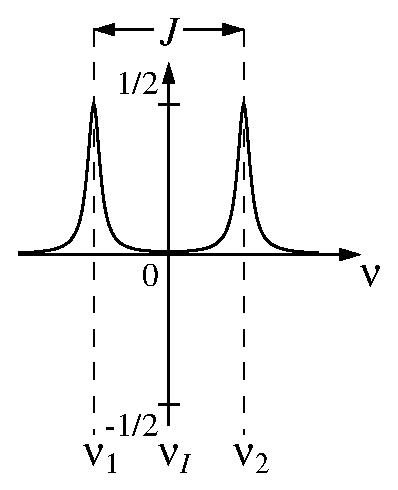
\epsfig{file=ix-is.eps,width=1.5in} \hspace{1cm}
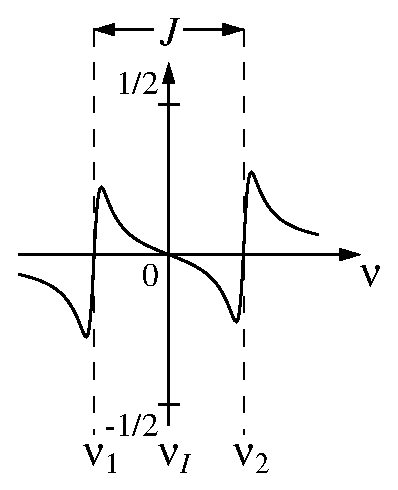
\epsfig{file=iy-is.eps,width=1.5in} \\[1cm]
\end{center}
\caption[Doublets produits par un système $IS$]{
\label{fig:ixy-is}
(a) doublet en absorption issu de $I_x$,
(b) doublet en dispersion issu de $I_y$}
\end{figure}

Si les noyaux $I$ et $S$ ne sont pas de même nature, 
l'impulsion qui excite par exemple l'aimantation du noyau $I$
est sans action sur le noyau $S$.
La détection aux fréquences de $I$ fait 
apparaître un doublet aux fréquences $\nu_1 = \nu_I + J/2$ et
$\nu_2 = \nu_I - J/2$ et rien n'est détectable dans la gamme des
fréquences de résonance de $S$.
Il suffit pour s'en convaincre d'éliminer du calcul
qui précède les termes qui disparaissent si l'opérateur
lié à l'impulsion est seulement $\pi/2 \cdot I_y $
au lieu de $\pi/2 \cdot (I_y + S_y)$.

Dans l'expérience impulsion-détection qui vient d'être décrite 
le signal dû au
noyau $I$ provient de l'évolution de $I_z$ et de $I_z$ uniquement. 
Ce sera toujours le cas pour ce type d'expérience quel que 
soit le nombre de noyaux couplés à $I$.

\section{Systèmes à trois spins (ou plus), faiblement couplés}

\subsection{Méthode}
Conformément à ce qui précède, il faut $4^3 =$ 64 matrices de base pour
décrire l'état d'un système $ISL$ où les trois noyaux sont couplés :

\begin{itemize}
\item La matrice identité $E$, sous forme $E/2$
\item $I_i$, $S_i$ et $L_i$ où $i$ vaut $x$, $y$ ou $z$ (9 matrices)
\item $2I_iS_j$, $2I_iL_j$, $2S_iL_j$ où $i$ et $j$ 
valent $x$, $y$ ou $z$ (27 matrices)
\item $4I_iS_jL_k$ où $i$,$j$ et $k$ valent $x$, $y$ ou $z$ (27 matrices)
\end{itemize}
L'état d'équilibre d'un tel système est défini par la matrice densité 
\begin{equation}
\sigma_0 = \Delta P(I)/4 \cdot I_z + \Delta P(S)/4 \cdot S_z + 
\Delta P(L)/4 \cdot L_z
\end{equation}
Cette écriture se simplifie si le système est homonucléaire : 
\begin{equation}
\sigma_0 = I_z + S_z + L_z
\end{equation}
et si l'aspect quantitatif des calculs qui suivent n'est pas
essentiel.

Les opérateurs associés aux impulsions d'angle $\theta$ sont 
$\epsilon \theta \cdot I_i$, où $i$ vaut $x$ 
ou $y$ et $\epsilon$ 1 ou $-1$ selon la phase de l'impulsion. 
Si plusieurs noyaux sont concernés par une 
impulsion (2 ou 3 noyaux sont de même nature), 
les opérateurs associés sont appliqués successivement.

Les opérateurs d'évolution associés aux déplacements chimiques de 
$I$, $S$ et $L$ sont $\omsi t \cdot I_z$, 
$\omss t \cdot S_z$ et $\omsl t \cdot L_z$. 
Les opérateurs associés au couplage scalaire sont les même que pour 
les systèmes à deux noyaux. 
Il n'existe pas de "super-couplage" qui ferait intervenir 
simultanément les trois noyaux et donc des opérateurs de type 
$4I_zS_zL_z$.

Les règles de commutation ont la même structure que celles utilisées 
pour les systèmes à deux spins. 
Ainsi, par exemple :
\begin{itemize}
\item $\{2I_zS_z,2S_xL_x\} = 4I_z\{S_z,S_x\}L_x = 4I_zS_yL_x$
\item $\{2I_zS_z,2S_zL_y\} = 4I_z\{S_z,S_z\}L_y = 0$
\item $\{2I_zS_z,4I_xS_yL_x\} = 2\{2I_zS_z,2I_xS_y\}L_x = 0$
\item $\{2I_zS_z,4I_xS_zL_y) = 2\{2I_zS_z,2I_xS_z\}L_y = 2I_yL_y$
\end{itemize}

Si par exemple, les noyaux $I$ et $L$ sont de même nature 
et que le signal est détecté à leur 
fréquence, $\aimxs$ (respectivement $\aimys$) est la somme des coefficients
multiplicatifs de $I_x$ et $L_x$  (respectivement $I_y$ et $L_y$).

\subsection{Exemple}
\label{sec:isl}
Considérons un noyau $I$ d'un certain type, couplé à des 
noyaux $S$ et $L$ d'un autre type.
Ce système est caractérisé par trois constantes de 
couplage : $J_{IS}$, $J_{IL}$ et $J_{SL}$. 
A titre d'exemple, considérons l'évolution du noyau $I$, 
soumis d'abord à une impulsion $\pi/2_y$, puis à 
une évolution libre pendant laquelle le signal est enregistré.

Initialement on considérera que $\sigma_0 = I_z$. 
Comme cela se vérifie aisément, seul ce terme fournira un signal détectable à 
la fréquence du noyau $I$.
L'opérateur associé à l'impulsion est comme précédemment $\pi/2 \cdot I_y$.
L'état $\sigma_0$ devient $\sigma_1 = I_x$.
L'opérateur d'évolution comprend 6 termes : $\omss t \cdot S_z$,
$\omsl t \cdot L_z$, $\pi J_{SL} t \cdot 2S_zL_z$, $\omsi t \cdot I_z$, 
$\pi J_{IS} t \cdot 2I_zS_z$ et $\pi J_{IL} t \cdot 2I_zL_z$.
Les trois premiers termes commutent avec $I_x$, il suffit donc d'appliquer les trois 
derniers à $I_x$ pour calculer $\sigma(t)$. 

Les calculs sont menés de façon commode lorsqu'ils 
sont présentés sous forme graphique, comme sur la figure \ref{fig:isl}. 
L'action d'un opérateur $\theta \cdot A$ qui commute avec une 
matrice de base $B$ se traduit par une double flèche verticale.
Dans le cas contraire une 
flèche vers la gauche mène à la copie de la matrice de base $B$ considérée 
et une flèche vers la droite mène au commutateur de l'opérateur et de la matrice de base,
c'est-à-dire à $\{A,B\}$. 
Une flèche à gauche est associée au facteur multiplicatif $\cos(\theta)$, 
une flèche à droite est associée à $\sin(\theta)$. 
Dans le cas où $\theta$ vaut $\pm \pi/2$ la flèche vers la droite est 
associée au coefficient nul ($\sin(\pm\pi/2)$), 
on ne trace alors qu'une simple flèche verticale.
Sur la droite du schéma sont indiqués les opérateurs qui interviennent
à chaque étape du calcul.

\begin{figure}[hbt]
\setlength{\unitlength}{0.9mm}
\begin{center}
\begin{picture}(160,80)
 
 \put(70,80){\makebox(0,0)[t]{$\boldsymbol{\sigma_0 = I_z}$}}
 
 \thicklines
 \put(70,76){\vector(0,-1){10}}
 \thinlines
  \put(160,70){\makebox(0,0)[rb]{$\pi/2 \cdot I_y$}}
 \put(70,65){\makebox(0,0)[t]{$\boldsymbol{\sigma_1 = I_x}$}}
 
 \thicklines
 \put(69.8,61){\vector(0,-1){10}} \put(70.2,61){\vector(0,-1){10}}
 \thinlines
  \put(160,55){\makebox(0,0)[rb]
   {$\omss t \cdot S_z + \omsl t \cdot L_z + \pi J_{SL} t \cdot 2S_zL_z$}}
 \put(70,50){\makebox(0,0)[t]{$\boldsymbol{I_x}$}}
 
 \thicklines
 \put(70,46){\vector(-4,-1){40}}
 \thinlines
 \put(70,46){\vector(4,-1){40}}
 \put(30,35){\makebox(0,0)[t]{$\boldsymbol{I_x}$}}
  \put(160,40){\makebox(0,0)[rb]{$\pi J_{IS} t \cdot 2I_zS_z$}}
 \put(110,35){\makebox(0,0)[t]{$2I_yS_z$}}
 
 \thicklines
 \put(30,31){\vector(-2,-1){20}}
 \thinlines
 \put(30,31){\vector(2,-1){20}}
 \put(110,31){\vector(-2,-1){20}}
 \put(110,31){\vector(2,-1){20}}
 \put(10,20){\makebox(0,0)[t]{$\boldsymbol{I_x}$}}
 \put(50,20){\makebox(0,0)[t]{$2I_yL_z$}}
 \put(90,20){\makebox(0,0)[t]{$2I_yS_z$}}
  \put(160,25){\makebox(0,0)[rb]{$\pi J_{IL} t \cdot 2I_zL_z$}}
 \put(130,20){\makebox(0,0)[t]{$-4I_xS_zL_z$}}
 
 \thicklines
 \put(10,16){\vector(-1,-1){10}}
 \put(10,16){\vector(1,-1){10}}
 \thinlines
 \put(50,16){\vector(-1,-1){10}}
 \put(50,16){\vector(1,-1){10}}
 \put(90,16){\vector(-1,-1){10}}
 \put(90,16){\vector(1,-1){10}}
 \put(130,16){\vector(-1,-1){10}}
 \put(130,16){\vector(1,-1){10}}

 \put(0,5){\makebox(0,0)[t]{$\boldsymbol{I_x}$}}
 \put(20,5){\makebox(0,0)[t]{$\boldsymbol{I_y}$}}
 \put(40,5){\makebox(0,0)[t]{$2I_yL_z$}}
 \put(60,5){\makebox(0,0)[t]{$-2I_xL_z$}}
 \put(80,5){\makebox(0,0)[t]{$2I_yS_z$}}
 \put(100,5){\makebox(0,0)[t]{$-2I_xS_z$}}
 \put(120,5){\makebox(0,0)[t]{$-4I_xS_zL_z$}}
  \put(160,10){\makebox(0,0)[rb]{$\omsi t \cdot I_z$}}
 \put(140,5){\makebox(0,0)[t]{$4I_yS_zL_z$}}

\end{picture}
\end{center}
 \caption[Évolution de $2I_x$, système $ISL$]{\label{fig:isl}
 Excitation et évolution libre de l'aimantation d'un noyau $I$
 couplé à deux noyaux $S$ et $L$.}
\end{figure}

Les parties du graphe en gras correspondent uniquement
à la partie utile.
Comme il est facile de s'en rendre compte, les termes de la
dernière ligne qui ne sont pas en gras ne contribuent pas
au signal.
Avec un peu d'habitude il est possible de savoir,
sans faire d'erreur, quelles branches de l'arbre n'ont
aucune chance d'aboutir à de l'aimantation mesurable.
Pour connaître $s_x(t)$ et $s_y(t)$ il suffit de partir de
la racine de l'arbre (située en haut !) et de faire le
produit des facteurs $\sin()$ et $\cos()$ qui aboutissent à
$I_x$ et $I_y$.

Ainsi,
\begin{eqnarray}
s_x(t) & = & \cos( \pi J_{IS} t) \cos(\pi J_{IL} t) \cos(\omsi t) \\
s_y(t) & = & \cos( \pi J_{IS} t) \cos(\pi J_{IL} t) \sin(\omsi t)
\end{eqnarray}

Le signal complexe $s(t)$ vaut donc
\begin{equation}
s(t) = \cos( \pi J_{IS} t) \cos(\pi J_{IL} t) \exp(i \omsi t)
\end{equation}

En transformant les cosinus en exponentielles complexes :
\begin{equation}
s(t) = \frac{1}{4}\exp(i \omsi t)
(\exp(i \pi J_{IS} t) + \exp(-i \pi J_{IS} t))
(\exp(i \pi J_{IL} t) + \exp(-i \pi J_{IL} t))
\end{equation}
dont le développement fournit une somme de 4 termes :
\begin{eqnarray}
s(t) & = & \frac{1}{4} \exp(i (\omsi + \pi J_{IS} + \pi J_{IL}) t) \\
& & + \frac{1}{4} \exp(i (\omsi + \pi J_{IS} - \pi J_{IL}) t) \\
& & + \frac{1}{4} \exp(i (\omsi - \pi J_{IS} + \pi J_{IL}) t) \\
& & + \frac{1}{4} \exp(i (\omsi - \pi J_{IS} - \pi J_{IL}) t)
\end{eqnarray}

La transformée de Fourier de ce signal comporte quatre raies aux fréquences :
\begin{eqnarray}
\nu_1 & = & \nu_I - J_{IS}/2 - J_{IL}/2 \\
\nu_2 & = & \nu_I - J_{IS}/2 + J_{IL}/2 \\
\nu_3 & = & \nu_I + J_{IS}/2 - J_{IL}/2 \\
\nu_4 & = & \nu_I + J_{IS}/2 + J_{IL}/2
\end{eqnarray}

Un tel ensemble de raies constitue un doublet de doublets, dont on peut
extraire les valeurs des constantes de couplage :
\begin{eqnarray}
J_{IS} & = & \nu_3 - \nu_1 = \nu_4 - \nu_2 \\
J_{IL} & = & \nu_2 - \nu_1 = \nu_4 - \nu_3
\end{eqnarray}

Le coefficient 1/4 indique que chaque raie est 4 fois moins intense qu'une raie issue d'un 
noyau non couplé, comme indiqué sur la figure \ref{fig:ix-isl}.

\begin{figure}[hbt]
\begin{center}
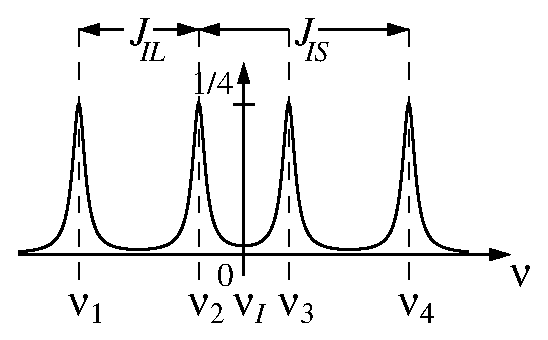
\epsfig{file=ix-isl.eps,width=1.5in}
\end{center}
\caption[Doublet de doublet produit par un système $ISL$]{
\label{fig:ix-isl}
Doublet de doublet produit par un système $ISL$}
\end{figure}

Si les constantes de couplage $J_{IS}$ et $J_{IL}$ sont égales,
on observe trois raies d'intensités 
relatives 1 : 2 : 1 qui constituent un triplet.

L'approximation des faibles couplages permet aussi de traiter les 
problèmes où deux noyaux sont magnétiquement équivalents, sous réserve de 
considérer comme nulle leur constante de couplage.

\section{Cohérences}

Le concept de "cohérence" est utilisé pour faciliter l'écriture des programmes
de phase associés aux séquences d'impulsions ou la mise en place
d'impulsions de gradient de champ statique $\bzerovec$.
Dans les deux cas il s'agit d'enregistrer la partie pertinente du signal
et d'éliminer celle que ne l'est pas.
Au paragraphe \ref{sec:progphaseft} nous avons vu que des imperfections
possibles de l'électronique de réception sont susceptibles
d'introduire des pics indésirables, pics
qui ont été éliminés en faisant varier simultanément les phases
d'émission (des impulsions) et de réception (du signal).
Ce besoin de tri sélectif du contenu du signal
est omniprésent dans les expériences de RMN multi--impulsionnelle.

Les cohérences sont définies de manière très naturelle à
partir de la définition de la matrice densité,
elles sont en fait liées à la manière dont on choisit une base
de matrices densité élémentaires pour décomposer la
matrice densité d'un système.
Cela va d'abord être illustré pour un système à un spin
et sera ensuite généralisé.

La base \{$E/2$, $I_x$, $I_y$, $I_z$\} peut être remplacée par la
base \{$E/2$, $I_+$, $I_-$, $I_z$\} où les matrices $I_+$ et $I_-$, sont 
définies par les relations :
\begin{equation}
I_+ = I_x + i \cdot I_y \qetq I_- = I_x - i \cdot I_y
\end{equation}
ou
\begin{equation}
I_x = \frac{I_+ + I_-}{2} \qetq I_y = \frac{I_+ - I_-}{2i}
\end{equation}

Les opérateurs $I_+$ et $I_-$ sont les cohérences du système à un spin.
Il est possible de voir ce que cela signifie en regardant
l'évolution de $\sigma_1 = I_x = (I_+ + I_-)/2$ 
sous l'action de l'opérateur d'évolution libre
$\phi \cdot I_z$ où $\phi = \omsi t$.
Ceci peut se faire en évaluant d'abord comment évoluent $I_+$ et $I_-$.
En ce qui concerne $I_+ = I_x + i \cdot I_y$ :
\begin{eqnarray}
I_+ & \flham{\phi \cdot I_z} & 
(\cos\phi \cdot I_x + \sin\phi \cdot I_y) + i(\cos\phi \cdot I_y - \sin\phi \cdot I_x) \\
& & = \cos\phi(I_x + i \cdot I_y) -i\sin\phi(I_x + i \cdot I_y) \\
\label{eqn:evoliplus} & & = \exp(-i \phi) \cdot I_+
\end{eqnarray}

De même,
\begin{equation}
\label{eqn:evolimoins}
I_- \flham{\phi \cdot I_z} \exp(+i \phi) \cdot I_-
\end{equation}

L'introduction de $\phi = \omsi t$ n'est pas seulement destinée
à alléger la présentation des calculs.
Elle introduit une unification formelle entre les rotations
de l'aimantation autour des axes transversaux du référentiel tournant
lors des impulsions de radio-fréquence et la rotation autour de l'axe $OZ$ pendant
les périodes de précession.

De manière générale \emph{une cohérence est une matrice densité qui est transformée
en un multiple d'elle même par action du superopérateur lié à
l'évolution libre du système}.
Un mathématicien dirait que les cohérences sont les matrices propres
du super--opérateur hamiltonien.

Pour en revenir à l'évolution de $I_x$, en remplaçant $\phi$ par sa valeur 
on obtient :
\begin{equation}
\label{eqn:evolcoher}
\sigma(t) = \exp(+i \omsi t)/2 \cdot I_- + \exp(-i \omsi t)/2 \cdot I_+
\end{equation}

Le signal observé est en fait le double du coefficient multiplicatif 
associé à la matrice de base $I_-$. 
Si le signal complexe $s(t)$ avait été calculé à partir de l'expression 
$M_x - i.M_y$, $s(t)$ aurait été le coefficient multiplicatif de $I_+$
(à un facteur 2 près).

La matrice densité $\sigma_1$ obtenue immédiatement après l'impulsion de radio-fréquence
traduit l'existence d'une aimantation transversale,
aimantation qui peut être convertie soit en signal évoluant à la pulsation $\omsi$, 
soit à la pulsation $-\omsi$.
Ceci est à rapprocher du fait que $\sigma_1 = I_+/2 + I_-/2$,
que $I_+$ évolue en $\exp(-i \omsi t) \cdot I_+$ et 
que $I_-$ évolue en $\exp(+i \omsi t) \cdot I_-$.
 
On associe aux matrices $I_-$ et $I_+$ une grandeur appelée ordre de 
cohérence (noté $p$) et qui vaut respectivement -1 et +1. 
L'ordre de cohérence $p$ d'une matrice traduit la manière 
dont elle évolue lors d'une rotation autour de $OZ$ : 
une matrice $B_p$ d'ordre bien défini $p$, comme $I_+$ et $I_-$, 
par opposition à $I_x$ et $I_y$ qui en sont des combinaisons,
évolue sous l'action d'un opérateur $\phi . I_z$ selon
\begin{equation}
B_p \flham{\phi \cdot I_z} \exp(-i p \phi) \cdot B_p
\end{equation}

La matrice $I_z$ reste invariante sous l'action des opérateurs d'évolution libre. 
Bien qu'elle ne soit pas associée à la mesure de l'aimantation transversale, on lui attribue 
formellement l'ordre 0 : $\exp(-i 0 \phi) = 1$, indépendamment de $\phi$.
La matrice identité $E$ se voit aussi attribuer un ordre de cohérence nul
du fait de son invariance par toute transformation linéaire.
Ces points seront détaillés ultérieurement, au paragraphe \ref{sec:population}.

L'ordre de cohérence $p$ d'une matrice est aussi couramment désigné sous le
terme "nombre de quanta" de l'état correspondant : 
$I_-$, $I_z$ et $I_+$ sont respectivement des états à -1, 0 (par extension) et +1 quanta.
Le fait que l'aimantation soit mesurée comme le facteur multiplicatif de $I_-$
fait dire que ce sont les états "à -1 quanta" qui sont observables.
Dans un système à un spin nous venons de voir que l'ordre
de cohérence d'un état d'ordre défini est invariante pendant une période
d'évolution libre.
Ce résultat est tout-à-fait général, tant que les phénomènes de relaxation
sont négligés.
Il est clair qu'au bout d'un temps infini l'état de tout système retourne vers
l'ordre 0.
Les impulsions de radio-fréquence sont le moyen par lequel le spectroscopiste
induit des changements d'ordre de cohérence du système et permet, entre autres,
la production d'aimantation transversale mesurable au cours de son retour à
l'équilibre.

\section{Ordre de cohérence et programme de phase}
\label{sec:progphasedensite}
Ce paragraphe fait appel aux notions introduites en \ref{sec:progphaseft}.

On y considère d'abord une impulsion d'angle $\pi/2$ et de phase 
nulle qui transforme $I_z$ ($p=0$) en $-I_y = -(I_+ - I_-)/2i$. 
Lors d'une seconde expérience, on augmente de $\pi/2$ la phase de 
l'impulsion pour former une impulsion $\pi/2_y$.
Cela peut se concevoir comme résultant de l'action successive
d'une impulsion $\pi/2_x$ exercée sur l'aimantation d'équilibre
suivie d'une rotation de $\pi/2$ autour de l'axe $OZ$,
et se justifie aisément en disant que l'axe de rotation $OX$ (première impulsion)
se transforme en $OY$ (seconde impulsion) par rotation de $\pi/2$
autour de $OZ$.
La première étape (l'impulsion $\pi/2_x$) conduit $I_z$ vers $-I_y = -(I_+ - I_-)/2i$.
La seconde étape (la rotation de $\pi/2$ autour de $OZ$)
transforme $I_+$ en $\exp(-i\pi/2) I_+ = -iI_+$
et $I_-$ en $\exp(+i\pi/2) I_- = iI_-$.
Globalement $I_z$ devient $-(-iI_+ - iI-)/2i$ soit $I_x$.

Ce raisonnement peut paraître superflu car le lecteur a remarqué depuis
un certain temps déjà qu'une impulsion $\pi/2_y$ transforme $I_z$ en $I_x$.
Son intérêt consiste à considérer dans son ensemble
les évènements de la séquence impulsion--détection.
L'état du système à la fin de la première impulsion est $-I_y = -(I_+ - I_-)/2i$,
ce qui conduit à $s(t=0)=-i$,
$-i$ étant le double du facteur multiplicatif de $I_-$ à la fin de l'impulsion.
Sachant que $I_-$ évolue en $\exp(-i(-1)\omsi t)I_- = \exp(i\Omega t)I_-$ 
après $t$ secondes,
le signal détecté après l'impulsion de phase nulle est $-i\exp(i\Omega t)$.
Si la phase de l'impulsion est maintenant augmentée de $\pi/2$, $I_-$ est remplacé
par $\exp(+i\pi/2) I_-$ au temps $t=0$ de la détection.
Le signal enregistré est donc simplement multiplié par $\exp(+i\pi/2) = i$,
comme déjà observé en \ref{sec:progphaseft}.
Il suffit de multiplier dans le récepteur le signal par $-i$ pour additionner
de manière constructive les signaux issus des deux impulsions.
Cette multiplication correspond, comme cela a déjà été dit, à une augmentation
$\Delta\phi_R = \pi/2$ de la phase du récepteur.

En retraçant l'origine du résultat, $\Delta\phi_R = \Delta\phi$,
que nous venons d'établir à nouveau, mais par des
moyens qui se prêtent aisément à une généralisation, il apparaît
que l'augmentation de la phase du récepteur doit être égale à la celle
de l'impulsion pour les raisons suivantes :
\begin{itemize}
\item L'aimantation initiale se comporte comme un état à 0 quanta
\item L'impulsion produit un état à -1 quanta
\item Cet état à -1 quanta initial restera à -1 quanta pendant la détection
\item Seul l'état à -1 quanta est détectable
\item L'impulsion produit aussi un état à +1 quanta
\item Cet état à +1 quanta reste à +1 quanta et n'est pas détectable
\item Une augmentation de la phase de l'impulsion de $\Delta\phi$ multiplie $s(t=0)$
par $\exp(-i p \Delta\phi) = \exp(i \Delta\phi)$ car $p(I_-)=-1$
\item $s(t)$ se déduit de $s(0)$ de manière indépendante de la nature de l'impulsion.
\item L'augmentation de la phase du récepteur de $\Delta\phi$ compense exactement
le facteur multiplicatif introduit par l'augmentation de la phase de l'impulsion.
\end{itemize} 

Le raisonnement tenu ici n'est valable que parce que l'aimantation initiale est
décrite par un état à 0 quanta et que l'état détecté est à -1 quanta.
Lorsque ce n'est pas le cas, un résultat analogue mais général peut être obtenu,
résultat qui lie phase du récepteur et phase de la ou des impulsions
de la séquence utilisée.
La démonstration en sera abordée lorsque les cohérences des systèmes
à plusieurs spins auront été définies.

Pour en finir avec ce paragraphe quelque peu théorique,
il est intéressant de voir quelle interprétation donner aux
pics axiaux et fantômes de quadrature dans le cadre du formalisme des cohérences.

Les pics axiaux apparaissent à l'identique quelle que soit
la phase de l'impulsion utilisée.
On peut donc dire que tout se passe comme si le détecteur enregistre
un signal constant, issu d'une cohérence à 0 quanta, associé à une pulsation nulle.

Rappelons que si les amplificateurs des signaux $s_x(t)$ et $s_y(t)$
ont des gains relatifs $1+\delta$ et $1-\delta$ le signal
observé est $s'(t)=\exp(i\omsi t) + \delta\exp(-i\omsi t)$,
ce qui correspond pour le premier terme à la détection normale des -1 quanta
et pour le second terme à la détection des +1 quanta.
Pour se convaincre de cette dernière affirmation, il suffit de se rappeler
que $\exp(-i\Omega t)$ est le facteur multiplicatif de $I_+$ lors de l'évolution
libre de l'aimantation transversale (équation \ref{eqn:evolcoher}).
Les signaux issus de la détection des +1 quanta sont multipliés
par $\exp(-i\pi/2) = -i$ lorsque la phase de l'impulsion est augmentée de $\pi/2$.
L'augmentation de $\pi/2$ de la phase du récepteur multiplie à son tour
le signal par $\exp(-i\pi/2) = -i$.
La contribution provenant de la détection des +1 quanta est donc multipliée
par $(-i)(-i)=-1$, et disparaît par addition des signaux.

Le programme de phase, en additionnant de manière constructive
que les signaux issus de la détection des -1 quanta, élimine
les signaux indésirables aux pulsations 0 et $-\omsi$.

\section{Évolution libre des matrices de base}

Le but de ce paragraphe est de préciser comment évoluent les 
matrices de base des systèmes à un ou plusieurs spins, afin de pouvoir prévoir rapidement 
quelle matrice de base, écrite au temps $t=0$ de l'acquisition du signal
sera responsable de quel groupe de raies dans le spectre.
Il constitue une extension de l'exemple du paragraphe \ref{sec:isl}
et permet d'introduire le concept de cohérence pour les systèmes à
plusieurs spins.

\subsection{Système à un spin, encore}
Dans un système à un spin, $\sigma(t=0) = I_x$ évolue pour donner le signal 
$s(t) = \exp(i \omsi t)$, 
dont la transformée de Fourier $S(\Omega) = A(\omsi) + iD(\omsi)$ a pour
partie réelle la courbe lorentzienne en 
absorption $A(\omsi)$ (figure \ref{fig:absorp}), 
si on tient compte du facteur de relaxation transversale. 
Dans les mêmes conditions, $I_y$ évolue pour donner un signal $s(t) = i\exp(i \omsi t)$
dont la transformée de Fourier $S(\Omega) = -D(\omsi) + iA(\omsi)$
a pour partie réelle la courbe de Lorentz en dispersion $-D(\omsi)$
(figure \ref{fig:dispers}).

\subsection{Système à deux spins}

\subsubsection{Etats non couplés}
L'évolution de $\sigma(t=0) = I_x$ pour un système à deux spins $IS$ 
faiblement couplés fournit le signal 
$2s(t) = \exp(i (\omsi + \pi J) t) + \exp(i (\omsi - \pi J) t)$. 
La partie réelle spectre 
\begin{equation}
S(\Omega) = A(\omsi + \pi J) + iD(\omsi + \pi J) + A(\omsi - \pi J) + iD(\omsi - \pi J)
\end{equation}
présente deux raies 
d'absorption aux pulsations $\omsi + \pi J$ et $\omsi - \pi J$.
Elles constituent un doublet en absorption et en phase.
Ce dernier terme indique que les deux parties du doublet sont de même signe.
Le spectre qui résulte de l'évolution de $I_y$, dans le mêmes conditions,
présente deux raies en dispersion et en phase. 
Les évolutions de $S_x$ et de $S_y$ sont semblables à celles de $I_x$ et $I_y$,
en remplaçant $\omsi$ par $\omss$.
Pour une raison qui apparaîtra au paragraphe suivant, les états
$I_x$, $I_y$, $S_x$ et $S_y$ sont dits "états non couplés" du système $IS$.

Reprenons la question de l'évolution libre de $\sigma(t=0) = I_x$ mais
avec une description utilisant les cohérences.
On peut à ce stade tenter d'écrire $I_+ = I_x + iI_y$ et $I_- = I_x - iIy$
en se rappelant qu'il s'agit de matrices à 16 éléments (4 fois 4) et non plus
de matrices à 4 éléments (2 fois 2) comme pour les systèmes à un spin.

$I_+$ est une matrice d'ordre de cohérence $+1$ 
si une rotation d'angle $\phi$ autour de $OZ$
donne $\exp(-i\phi)I_+$.
Une rotation autour de $OZ$ et d'angle $\phi$ correspond dans ce contexte
au superopérateur associé à l'opérateur $\phi F_z$ où 
\begin{equation}
\label{eqn:operateurf}
F_z = I_z + S_z
\end{equation}
et autrement dit, à l'opérateur $\phi I_z + \phi S_z$.
Etant donné que $\{S_z, I_{\pm}\} = 0$, 
les matrices $I_+$ et $I_-$ sont transformées
en $\exp(-i \phi) I_+$ et $\exp(i \phi) I_-$ par action de $\phi F_z$,
ce qui leur confère respectivement un ordre de cohérence $+1$ et $-1$.

\subsubsection{États couplés}
Il est possible d'écrire $2I_xS_z = (I_+ + I_-)Sz = I_+S_z + I_-S_z$
et facile à vérifier que $I_+S_z$ et $I_-S_z$ sont aussi des matrices respectivement
d'ordre de cohérence +1 et -1 puisque $\{S_z, 2I_{x,y}S_z\} = 0$ et 
$\{I_z, 2I_{x,y}S_z\} = 2\{Iz, I_{x,y}\}S_z$.

L'évolution de $2I_xS_z$ sous l'action de l'opérateur d'évolution libre
$H = \omsi t I_z + \omss t S_z + \pi J t 2I_zS_z$ est décrite par la figure
\ref{fig:evolixsz}.

\begin{figure}[hbt]
\begin{center}
\setlength{\unitlength}{0.9mm}
\begin{picture}(80,50)
 
 \put(0,5){\makebox(0,0)[t]{$2I_xS_z$}}
 \put(20,5){\makebox(0,0)[t]{$2I_yS_z$}}
 \put(40,5){\makebox(0,0)[t]{$\boldsymbol{I_y}$}}
 \put(60,5){\makebox(0,0)[t]{$\boldsymbol{-I_x}$}}
  \put(80,10){\makebox(0,0)[rb]{$\omsi t \cdot I_z$}}
 \put(10,16){\vector(-1,-1){10}}
 \put(10,16){\vector(1,-1){10}}
 \thicklines
 \put(50,16){\vector(-1,-1){10}}
 \put(50,16){\vector(1,-1){10}}
 \thinlines

 \put(10,20){\makebox(0,0)[t]{$2I_xS_z$}}
 \put(50,20){\makebox(0,0)[t]{$\boldsymbol{I_y}$}}
  \put(80,25){\makebox(0,0)[rb]{$\pi J_{IL} t \cdot 2I_zS_z$}}
 \put(30,31){\vector(-2,-1){20}}
 \thicklines
 \put(30,31){\vector(2,-1){20}}
 \thinlines

 \put(30,35){\makebox(0,0)[t]{$\boldsymbol{2I_xS_z}$}}
  \put(80,40){\makebox(0,0)[rb]{$\omss t \cdot 2S_z$}}
 \thicklines
 \put(29.8,46){\vector(0,-1){10}} \put(30.2,46){\vector(0,-1){10}}
 \thinlines

 \put(30,50){\makebox(0,0)[t]{$\boldsymbol{2I_xS_z}$}}

\end{picture}
 \caption[Évolution de $2I_xS_z$, système $IS$]{\label{fig:evolixsz} 
 Évolution libre d'un état $2I_xS_z$ d'un système $IS$.}
\end{center}
\end{figure}

Contrairement à ce qui se passe pour l'évolution de $I_x$ où, à la fin du calcul, 
le coefficient multiplicatif de $I_x$ et $I_y$ varie en $\cos(\pi J t)$, 
ici ces coefficient varient en $\sin(\pi J t)$. 
Ainsi 
\begin{eqnarray}
s(t) & = & -\sin(\omsi t)\sin(\pi J t) + i\cos(\omsi t)\sin(\pi J t) \\
& = & i\exp(i\omsi t)\sin(\pi J t)
\end{eqnarray}
Le développement de la fonction sinus en exponentielles complexes :
\begin{equation}
s(t) = \exp(i (\omsi t + \pi J)t)/2 - \exp(i (\omsi t - \pi J)t)/2
\end{equation}
fait apparaître deux raies en absorption mais de signes opposés :
on parle alors d'un doublet antiphase. 
Il en est de même pour $2I_zS_x$, $2I_yS_z$ et $2I_zS_y$
Ces matrices de base décrivent des états du système appelés "états couplés".

La figure \ref{fig:ixysz-is} montre les doublets produits par un noyau
$I$ couplé faiblement à partir des états (a) $2I_xS_z$ et (b) $2I_yS_z$.

\begin{figure}[hbt]
\begin{center}
$a$\hspace{1.5in}\hspace{1cm}$b$\hspace{1.5in}$\mbox{ }$\\
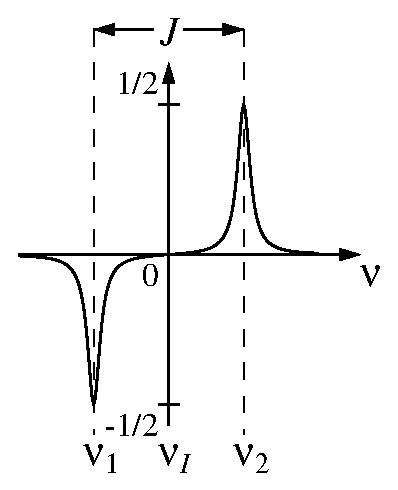
\epsfig{file=ixsz-is.eps,width=1.5in} \hspace{1cm}
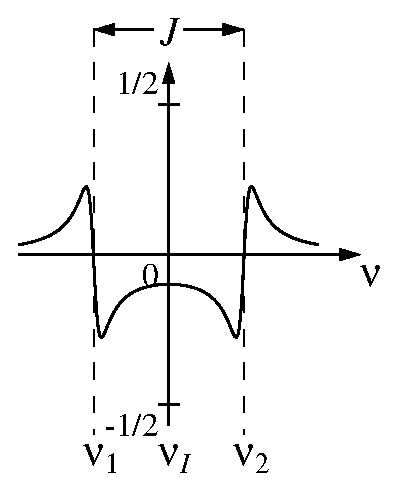
\epsfig{file=iysz-is.eps,width=1.5in}
\end{center}
\caption[Doublets antiphases produits par un système $IS$]{
\label{fig:ixysz-is}
(a) doublet antiphase en absorption issu de $I_xS_z$,
(b) doublet antiphase en dispersion issu de $I_yS_z$}
\end{figure}

Les états $I_-$ et $I_-S_z$ sont, nous l'avons vu, des matrices
d'ordre de cohérence -1.
Ils se convertissent l'un en l'autre par action de l'opérateur
d'évolution libre mais conservent donc l'ordre de cohérence -1 :
\begin{eqnarray}
I_x & \flham{\pi J t \cdot 2I_zSz} &
\cos(\pi J t) \cdot I_x + \sin(\pi J t) \cdot 2I_yS_z \\ 
I_y & \flham{\pi J t \cdot 2I_zSz} &
\cos(\pi J t) \cdot I_y - \sin(\pi J t) \cdot 2I_yS_z
\end{eqnarray}
D'où
\begin{eqnarray}
I_{\pm} = I_x \pm iI_y & \flham{\pi J t \cdot 2I_zSz} &
\cos(\pi J t) \cdot I_{\pm} \mp i \sin(\pi J t) \cdot 2I_{\pm}S_z \\
\label{eqn:evolipm-is} I_{\pm} & \flham{Ht} &
\exp(\mp i \omsi t)(\cos(\pi J t) \cdot I_{\pm} \mp i \sin(\pi J t) \cdot 2I_{\pm}S_z)
\end{eqnarray}
De manière identique :
\begin{equation}
\label{eqn:evolipmsz-is} 2I_{\pm}S_z \flham{Ht}
\exp(\mp i \omsi t)(\cos(\pi J t) \cdot 2I_{\pm}S_z \mp i \sin(\pi J t) \cdot I_{\pm})
\end{equation}

Les matrices $I_{\pm}$ et $2I_{\pm}S_z$ ne sont pas des cohérences du 
système étudié, toutefois leur ordre de cohérence n'est pas modifié
par l'évolution libre, puisqu'elles évoluent comme une somme de
deux matrices de même ordre de cohérence.

Ce résultat est très général : \emph{l'évolution libre de fait pas varier
l'ordre de cohérence d'un état}.

A partir de la demi somme et de la demi différence des équations 
\ref{eqn:evolipm-is} et \ref{eqn:evolipmsz-is},
du fait que $I_{\pm}$ est en fait $I_{\pm}E_S$,
et des définitions :
\begin{eqnarray}
S_{\al} & = & \frac{E_S + 2S_z}{2} \\
S_{\be} & = & \frac{E_S - 2S_z}{2}
\end{eqnarray}
on obtient
\begin{eqnarray}
\label{eqn:evolipmsa-is} I_{\pm}S_{\al} & \flham{Ht} &
\exp(\mp i (\omsi + \pi J)t) \cdot I_{\pm}S_{\al} \\
\label{eqn:evolipmsb-is} I_{\pm}S_{\be} & \flham{Ht} &
\exp(\mp i (\omsi - \pi J)t) \cdot I_{\pm}S_{\be}
\end{eqnarray}
ce qui prouve que les matrices $I_{\pm}S_{\al}$ et $I_{\pm}S_{\be}$ 
sont des cohérences du système $IS$ faiblement couplés,
d'ordre de cohérence $\pm 1$.
Il en est de même, par symétrie, pour les matrices $I_{\al}S_{\pm}$ et $I_{\be}S_{\pm}$.

Les fréquences d'évolution de ces cohérences à simple quanta sont exactement les
fréquences des transitions observables dans le diagramme énergétique du système $IS$.
L'ordre de cohérence d'un terme de la matrice densité
correspond de fait à la valeur de $\Delta m_s$ de la transition qui lui est associée.
Ce point est à la base du lien qui sera fait entre le formalisme
de la matrice densité et la généralisation du modèle de Bloch.

\subsubsection{États à 0 et double quanta}
Parmi les états dont il n'a pas encore été question figurent ceux décrits
par les opérateurs $2I_{x,y}S_{x,y}$.
Le fait est qu'ils sont impossibles à produire à partir de l'état d'équilibre
en utilisant une seule impulsion idéale, ce qui
explique qu'ils n'aient pas encore été rencontrés avant ce point du texte.
Ils sont cependant impliqués dans certaines expériences multi--impulsionnelles
de grande importance pratique.
La matrice $2I_xS_x$ s'exprime en fonction de $I_+$, $I_-$, $S_+$, $S_-$
par la relation $2I_xS_x = (I_+ + I_-)(S_+ + S_-)/2$ soit 
$I_+S_+/2 + I_+S_-/2 + I_-S_+/2 + I_-S_-/2$. 

A nouveau l'action de l'opérateur $\phi \cdot F_z$ sur ces quatre derniers
opérateurs montre que ce sont des cohérences d'ordre respectivement +2, 0, 0 et -2.
On parle alors de cohérence à double et à zero quanta.
Il est donc certain que l'évolution libre de $2I_xS_x$ ne fera apparaître 
aucune aimantation mesurable.
La matrice $2I_xS_x$ évolue néanmoins, mais sans faire apparaître la constante de 
couplage puisque $2I_zS_z$ et $2I_xS_x$ commutent, comme
indiqué sur la figure \ref{fig:evolixsx}.

\begin{figure}[hbt]
\begin{center}
\setlength{\unitlength}{0.9mm}
\begin{picture}(80,50)
 
 \put(0,5){\makebox(0,0)[t]{$2I_xS_x$}}
 \put(20,5){\makebox(0,0)[t]{$2I_xS_y$}}
 \put(40,5){\makebox(0,0)[t]{$2I_yS_x$}}
 \put(60,5){\makebox(0,0)[t]{$2I_yS_y$}}
  \put(80,10){\makebox(0,0)[rb]{$\omss t \cdot S_z$}}
 \put(10,16){\vector(-1,-1){10}}
 \put(10,16){\vector(1,-1){10}}
 \put(50,16){\vector(-1,-1){10}}
 \put(50,16){\vector(1,-1){10}}

 \put(10,20){\makebox(0,0)[t]{$2I_xS_x$}}
 \put(50,20){\makebox(0,0)[t]{$2I_yS_x$}}
  \put(80,25){\makebox(0,0)[rb]{$\omsi t \cdot I_z$}}
 \put(30,31){\vector(-2,-1){20}}
 \put(30,31){\vector(2,-1){20}}

 \put(30,35){\makebox(0,0)[t]{$2I_xS_x$}}
  \put(80,40){\makebox(0,0)[rb]{$\pi J t \cdot 2I_zS_z$}}
 \put(29.8,46){\vector(0,-1){10}} \put(30.2,46){\vector(0,-1){10}}

 \put(30,50){\makebox(0,0)[t]{$2I_xS_x$}}

\end{picture}
 \caption[Evolution de $2I_xS_x$, système $IS$]{\label{fig:evolixsx} 
 Evolution libre d'un état $2I_xS_x$ d'un système $IS$.}
\end{center}
\end{figure}

Dans $\sigma(t)$, le coefficient multiplicatif de $2I_xS_x$ est 
$\cos(\omsi t) \cos(\omss t)$, qui vaut aussi 
$\cos((\omsi + \omss)t)/2 + \cos((\omsi - \omss)t)/2$. 
Les pulsations $\omsi + \omss$ et $\omsi - \omss$ sont les 
pulsations associées aux transitions à $\pm 2$ et 0 quanta du système $IS$. 
Un calcul identique montre que chacune des quatre matrices associées aux transitions à  
0 et $\pm 2$ quanta évolue pour donner des combinaisons de ces quatre matrices.
Cette observation est compatible avec la décomposition des matrices 
$2I_{x,y}S_{x,y}$ en termes d'ordre de cohérence 0 et $\pm 2$.
En effet, on peut écrire :
\begin{eqnarray}
& & I_{\pm}S_{\pm} \flham{\pi J t \cdot 2I_zS_z} I_{\pm}S_{\pm} \nonumber\\
& & \quad \flham{\omsi t I_z} 
\exp(i\mp\omsi t)I_{\pm}S_{\pm} \nonumber\\
& & \quad \flham{\omss t S_z}
\exp(i\mp\omsi t) \exp(i\mp\omss t) I_{\pm}S_{\pm} \nonumber\\
& & \quad\quad = \exp(i(\mp\omsi \mp\omss)t) I_{\pm}S_{\pm} 
\end{eqnarray}

Il apparaît donc ici que les matrices $I_{\pm}S_{\pm}$ sont des cohérences.
Leur fréquence d'évolution est égale aux fréquences des transitions
à zéro et double quanta déduites du diagramme énergétique du système $IS$.

\subsubsection{Ordres de cohérence partiels}
On constate que l'ordre de cohérence d'un état s'obtient par addition des ordres
de cohérence individuels associés aux noyaux $I$ et $S$ considérés séparément.
En fait, considérons une cohérence générale $I_{\lambda}S_{\mu}$, avec $\lambda$, $\mu$
valant $z$, $+$, $-$, ou 0 pour signifier que l'opérateur n'y figure pas
(et donc d'ordre de cohérence nul !).
Alors,
\begin{eqnarray}
& &I_{\lambda}S_{\mu} \flham{\phi \cdot Iz}
\exp(-i p(I_{\lambda}) \phi) \cdot I_{\lambda}S_{\mu}\\
& &I_{\lambda}S_{\mu} \flham{\phi \cdot Sz}
\exp(-i p(S_{\mu}) \phi) \cdot I_{\lambda}S_{\mu}\\
& &I_{\lambda}S_{\mu} \flham{\phi \cdot Fz}
\exp(-i p(I_{\lambda} \phi)\exp(-i p(S_{\mu}) \phi) \cdot I_{\lambda}S_{\mu}\nonumber\\
& & \quad = \exp(-i (p(I_{\lambda})+p(S_{\mu})) \phi) \cdot I_{\lambda}S_{\mu}
\end{eqnarray}
ce qui montre bien que
\begin{equation}
p(I_{\lambda}S_{\mu}) = p(I_{\alpha}) + p(S_{\mu})
\end{equation}

Les quantités $p(I_{\lambda})$ et $p(S_{\mu})$ sont appelées ordres de cohérence partiels,
quantités dont la somme est l'ordre de cohérence total.
Il est important aussi de noter que, dans la mesure où on ne considère
que des systèmes de spins faiblement couplés,
\emph{les ordres de cohérence partiels sont invariants au cours des périodes
d'évolution libre}. 

\subsubsection{Populations}
Les matrices $E$, $I_z$, $S_z$, $2I_zS_z$ sont invariantes par action des opérateurs 
d'évolution libre et ne sont sujettes qu'aux phénomènes liés à la relaxation longitudinale.
Ces matrices ne constituent pas des cohérences mais des populations (voir \ref{sec:population}),
bien que leur invariance sous l'action de $\phi \cdot F_z$ permettent de leur
attribuer un ordre de cohérence global nul, somme d'ordres de cohérence partiels nuls.

Il faut bien noter qu'un état comme $I_+S_-$, bien que d'ordre de cohérence nul,
n'est pas une population, car il n'est pas invariant par action de $\phi \cdot F_z$.

\subsection{Système à trois spins}
Les matrices de base utilisées pour décrire les systèmes à trois spins sont classables en 
sept catégories suivant les ordres de cohérences qui leur sont associés et l'existence 
d'états couplés.
Pour chaque catégorie nous donnerons dans la table \ref{tab:isl}
un exemple représentatif et la 
possibilité ou non de donner de l'aimantation observable
par évolution libre.

\begin{table}[hbt]
\begin{center}
\begin{tabular}{llcc}
 & Catégorie & Exemple & Détectable\\[0.5ex] 
1 & Population (pseudo-ordre 0) & $4I_zS_zL_z$ & non \\
2 & Ordre $\pm 1$ non couplé & $L_x$ & oui \\
3 & Ordre $\pm 1$ couplé 1 fois & $2S_zL_x$ & oui \\
4 & Ordre $\pm 1$ couplé 2 fois & $4I_xL_zS_z$ & oui \\
5 & Ordre 0, $\pm 2$ non couplé & $2S_xL_y$ & non \\
6 & Ordre 0, $\pm 2$ couplé & $4I_xS_yL_z$ & non \\
7 & Ordre $\pm 1$, $\pm 3$ & $4I_xS_xL_x$ & non
\end{tabular}
\caption{\label{tab:isl}Classification des opérateurs pour les systèmes à trois spins}
\end{center}
\end{table}

Les catégories originales introduites à cause de la présence d'un troisième noyau sont 
numérotées 4, 6 et 7.

Il convient d'insister ici sur le fait que l'état $2S_zL_x$,
ligne 3 du tableau \ref{tab:isl},
n'est pas détectable en tant que tel, mais que son évolution libre conduit
à un état observable.
Il en est de même pour les états correspondants à la ligne 4.

Considérons l'évolution des matrices $I_x$ (type 2), $2I_xS_z$ (type 3)
et $4I_xS_zL_z$ (type 4) selon l'opérateur 
d'évolution libre associé aux systèmes de trois noyaux faiblement couplés. 
Ces trois matrices commutent avec les opérateurs 
$\omss t \cdot S_z$, $\omsl t \cdot L_z$ et $\pi J_{SL} t \cdot 2S_zL_z$.
De plus, on ne s'intéresse qu'à la nature des résonances du noyau $I$ couplé à S et L, 
qui doit être indépendante de l'offset de $I$, ce qui permet de choisir $\omsi = 0$. 
Ceci revient à ne pas prendre en compte l'opérateur $\omsi t \cdot I_z$
Parmi les 6 termes initiaux de l'opérateur d'évolution libre,
seuls $\pi J_{IS} t \cdot 2I_zS_z$ et $\pi J_{IL} t \cdot 2I_zL_z$ restent à considérer.

Le calcul de l'évolution de $I_x$ a déjà été présenté en \ref{sec:isl}
et conduit à quatre raies en absorption de même signe (on dit aussi "en phase").

L'évolution de $2I_xS_z$ s'écrit :

\begin{figure}[hbt]
\begin{center}
\setlength{\unitlength}{0.9mm}
\begin{picture}(90,35)
 
 \put(0,5){\makebox(0,0)[t]{$2I_xS_z$}}
 \put(20,5){\makebox(0,0)[t]{$4I_yS_zL_z$}}
 \put(40,5){\makebox(0,0)[t]{$\boldsymbol{I_y}$}}
 \put(60,5){\makebox(0,0)[t]{$-2I_xL_z$}}
  \put(90,10){\makebox(0,0)[rb]{$\pi J_{IL} t \cdot 2I_zL_z$}}
 \put(10,16){\vector(-1,-1){10}}
 \put(10,16){\vector(1,-1){10}}
 \thicklines
 \put(50,16){\vector(-1,-1){10}}
 \thinlines
 \put(50,16){\vector(1,-1){10}}

 \put(10,20){\makebox(0,0)[t]{$2I_xS_z$}}
 \put(50,20){\makebox(0,0)[t]{$\boldsymbol{I_y}$}}
  \put(90,25){\makebox(0,0)[rb]{$\pi J_{IS} t \cdot 2I_zS_z$}}
 \put(30,31){\vector(-2,-1){20}}
 \thicklines
 \put(30,31){\vector(2,-1){20}}
 \thinlines
 
 \put(30,35){\makebox(0,0)[t]{$\boldsymbol{2I_xS_z}$}}

\end{picture}
 \caption[Evolution de $2I_xS_z$, système $ISL$]{\label{fig:evolixszl0} 
 Evolution libre d'un état $2I_xS_z$ d'un système $ISL$.}
\end{center}
\end{figure}

Ainsi
\begin{eqnarray}
s(t) & = & i\sin(\pi J_{IS} t)\cos(\pi J_{IL} t)\\
& = & i \sin(\pi(J_{IS}+J_{IL})t)/2 + i \sin(\pi(J_{IS}-J_{IL})t)/2
\end{eqnarray}

En transformant les fonctions sinus en exponentielles complexes
et après transformation de Fourier,
on obtient quatre raies en absorption de fréquences et d'intensités indiquées ci-dessous :
\begin{eqnarray*}
\mbox{Fréquence} & & \mbox{Intensité} \\[0.5ex]
+J_{IS}+J_{IL} & & +1/4 \\
+J_{IS}-J_{IL} & & +1/4 \\
-J_{IS}+J_{IL} & & -1/4 \\
-J_{IS}-J_{IL} & & -1/4 
\end{eqnarray*}

On retrouve $J_{IS}$ entre deux raies en antiphase et $J_{IL}$ entre deux raies en phase. 
Dans cet exemple $J_{IS}$ est appelé couplage actif car il intervient 
dans l'évolution de $2I_xS_z$ à la fois sur $I_x$ et sur $S_z$.
$J_{IL}$ est ici un couplage inactif (ou passif) : il n'intervient dans l'évolution de 
$2I_xS_z$ que sur $I_x$. 
Un couplage actif donne lieu à une paire de pics antiphase alors 
qu'un couplage inactif donne lieu à une paire de raies en phase.

L'évolution de $I_x$ ne conduit qu'à des pics en phase 
puisque tous les couplages sont passifs.

Dans l'évolution de $4I_xS_zL_z$ les constantes de couplage 
$J_{IL}$ et $J_{IS}$ sont toutes deux actives :

\begin{figure}[hbt]
\begin{center}
\setlength{\unitlength}{0.9mm}
\begin{picture}(90,35)
 
 \put(0,5){\makebox(0,0)[t]{$4I_xS_zL_z$}}
 \put(20,5){\makebox(0,0)[t]{$2I_yL_z$}}
 \put(40,5){\makebox(0,0)[t]{$2I_yS_z$}}
 \put(60,5){\makebox(0,0)[t]{$\boldsymbol{-2I_x}$}}
  \put(90,10){\makebox(0,0)[rb]{$\pi J_{IS} t \cdot 2I_zS_z$}}
 \put(10,16){\vector(-1,-1){10}}
 \put(10,16){\vector(1,-1){10}}
 \put(50,16){\vector(-1,-1){10}}
 \thicklines
 \put(50,16){\vector(1,-1){10}}
 \thinlines

 \put(10,20){\makebox(0,0)[t]{$4I_xS_zL_z$}}
 \put(50,20){\makebox(0,0)[t]{$\boldsymbol{2I_yS_z}$}}
  \put(90,25){\makebox(0,0)[rb]{$\pi J_{IL} t \cdot 2I_zL_z$}}
 \put(30,31){\vector(-2,-1){20}}
 \thicklines
 \put(30,31){\vector(2,-1){20}}
 \thinlines
 
 \put(30,35){\makebox(0,0)[t]{$\boldsymbol{4I_xS_zL_z}$}}

\end{picture}
 \caption[Évolution de $4I_xS_zL_z$, système $ISL$]{\label{fig:evolixszlz} 
 Évolution libre d'un état $4I_xS_zL_z$ d'un système $ISL$.}
\end{center}
\end{figure}

Ainsi,
\begin{eqnarray}
s(t) & = & -\sin(\pi J_{IS} t)\sin(\pi J_{IL} t)\\
& = & \cos(\pi(J_{IS}+J_{IL})t)/2 - \cos(\pi(J_{IS}-J_{IL})t)/2
\end{eqnarray}
En transformant les fonctions cosinus en exponentielles complexes
et après transformation de Fourier,
on obtient quatre raies en absorption de fréquences et d'intensités indiquées ci-dessous :
\begin{eqnarray*}
\mbox{Fréquence} & & \mbox{Intensité} \\[0.5ex]
+J_{IS}+J_{IL} & & +1/4 \\
+J_{IS}-J_{IL} & & -1/4 \\
-J_{IS}+J_{IL} & & -1/4 \\
-J_{IS}-J_{IL} & & +1/4 
\end{eqnarray*}
Les pics distants de $J_{IS}$ d'une part et de $J_{IL}$
d'autre part sont bien en antiphase.

La figure \ref{fig:ixzz-isl} montre les doublets de doublets produits par un noyau
$I$ couplé faiblement aux noyaux $S$ et $L$ à partir des états (a) $2I_xS_z$
et (b) $4I_xS_zL_z$.

\begin{figure}[hbt]
\begin{center}
$a$\hspace{1.5in}\hspace{1cm}$b$\hspace{1.5in}$\mbox{ }$\\
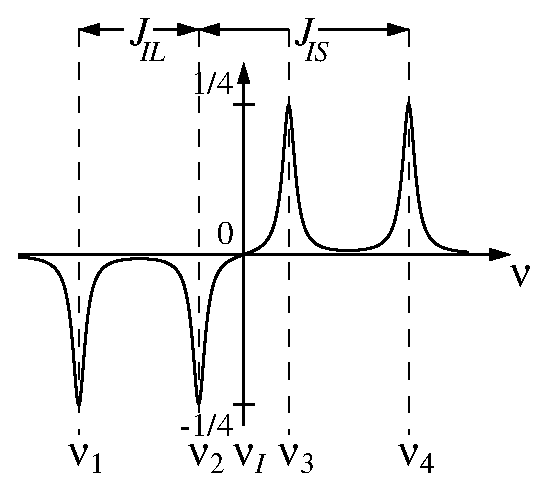
\epsfig{file=ixsz-isl.eps,width=1.5in} \hspace{1cm}
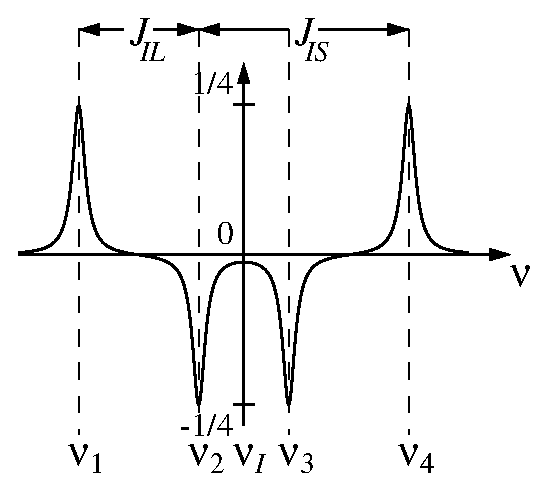
\epsfig{file=ixszlz-isl.eps,width=1.5in}
\end{center}
\caption[Doublets de doublets produits par un système $ISL$]{
\label{fig:ixzz-isl}
(a) Doublet de doublet issu de $2I_xL_z$, antiphase pour $S$ 
(b) doublet de doublet issu de $4I_xS_zL_z$, doublement antiphase (pour $S$ et $L$)}
\end{figure}

Il est intéressant de noter qu'une matrice de base 
comme $4I_xS_xL_x$ ne donne aucune aimantation 
observable alors qu'elle s'exprime aussi comme 
$(I_+ + I_-)(S_+ + S_-)(L_+ + L_-)/2$ et 
contient donc des termes comme $I_+S_-L_-$ d'ordre de cohérence total
égal à $-1$. 
L'existence d'un terme d'ordre de cohérence $-1$ est en effet une condition nécessaire 
mais non suffisante à l'obtention d'un signal.
La production d'un signal détectable reste l'exclusivité des opérateurs
$I_-$, $S_-$ et $L_-$.

\section{Populations} 
\label{sec:population}

\subsection{Systèmes à un spin}
\label{sec:popun}
Un ensemble de $P$ spins isolés en état d'équilibre dans le champ $\bzerovec$
est décrit par la matrice densité initiale
\begin{equation}
\sigma_0 = P \cdot E/2 + \Delta P \cdot I_z
\end{equation}
où 
\begin{equation}
P = p_{\al} + p_{\be} \qetq \Delta P = p_{\al} - p_{\be}
\end{equation}
en faisant intervenir
les populations associées aux niveaux énergétiques $E_{\al}$ et $E_{\be}$.
Ces populations sont aisément déductibles à partir des coefficients
de $E/2$ (qui est toujours égale à $P$) et de $I_z$ :
\begin{equation}
p_{\al} = \frac{P + \Delta P}{2} \qetq p_{\be} = \frac{P + \Delta P}{2}
\end{equation}

D'une manière générale, si
\begin{equation}
\sigma = a \cdot E/2 + b \cdot I_x + c \cdot I_y + d \cdot I_z
\end{equation}
alors
\begin{equation}
p_{\al} = \frac{a+d}{2} \qetq p_{\be} = \frac{a-d}{2}
\end{equation}
ce qui impose à $a$ et $d$ d'être des nombres réels.

L'invariance de $E/2$ et de $I_z$ sous l'action de l'opérateur
d'évolution libre entraîne l'invariance les populations des
états énergétiques pendant ces périodes, en l'absence de relaxation
longitudinale.

Une impulsion d'angle $\theta$ et de phase quelconque
exercée sur un système en équilibre transforme $I_z$ en
$\cos\theta \cdot I_z + ...$ et conduit donc à
\begin{equation}
p_{\al} = P\frac{1+\cos\theta}{2} \qetq
p_{\be} = P\frac{1-\cos\theta}{2}
\end{equation}
avec pour conséquence que si $\theta = \pi / 2$, alors les populations
sont égales et la composante longitudinale de l'aimantation est nulle
(certains auteurs parlent alors de saturation, même si l'aimantation
transversale est non nulle).
Une impulsion d'angle de nutation $\pi$ échange $p_{\al}$ et $p_{\be}$,
conduisant à ce qui est désigné par "inversion de population".
Le retour à l'équilibre est alors uniquement assuré par
la relaxation longitudinale (en négligeant le "radiation damping"...).
L'inversion de population offre donc un moyen, parmi d'autres, de mesurer
le temps de relaxation $T_1$ d'un système.

Notons qu'il est aussi possible d'écrire
\begin{equation}
\sigma = \frac{a+d}{2} \cdot \frac{E + 2I_z}{2} + \frac{a-d}{2} \cdot \frac{E - 2I_z}{2}
+ b \cdot I_x + c \cdot I_y
\end{equation}
qui, en introduisant les matrices
\begin{equation}
I_{\al} = \frac{E + 2I_z}{2} \qetq I_{\be} = \frac{E - 2I_z}{2}
\end{equation}
se transforme en
\begin{equation}
\sigma = p_{\al} \cdot I_{\al} + p_{\be} \cdot I_{\be} + b \cdot I_x + c \cdot I_y
\end{equation}

Le choix de $I_{\al}$ et $I_{\be}$ comme matrices de base au lieu de $E/2$ et $I_z$
donne directement accès aux populations des différents états énergétiques
possibles pour les noyaux.
Ces opérateurs sont pour cette raison appelés opérateurs de population.
L'écriture de $\sigma$ sous la forme:
\begin{equation}
\sigma = p_{\al} \cdot I_{\al} + p_{\be} \cdot I_{\be} 
+ \frac{b-ic}{2} \cdot I_+ + \frac{b+ic}{2} \cdot I_-
\end{equation}
présente la matrice densité comme combinaison linéaire des opérateurs
de population et des cohérences, représentation qui est la
plus "naturelle" (un mathématicien dirait "canonique")
d'après la définition de la matrice densité d'un système.
Toutefois, la simplicité des règles de calcul est en faveur de l'emploi de la
base des opérateurs cartésiens pour l'étude de l'évolution de $\sigma$
sous l'action des hamiltoniens usuels (évolution libre et impulsions de
radio-fréquence).

\subsection{Systèmes à deux spins}

Dans les systèmes à deux spins $IS$, quatre populations 
$p_{\al\al}$, $p_{\al\be}$, $p_{\be\al}$ et $p_{\be\be}$ sont à 
considérer, correspondant chacune à un état $m_s = \pm 1/2$ pour chaque noyau du système.  
Dans un cas général, la matrice densité contient l'information relative aux populations par 
l'intermédiaire des termes proportionnels à $E/2$, $I_z$, $S_z$ et $2I_zS_z$.
Si l'état du système est décrit par
\begin{equation}
\sigma = a_{E/2} \cdot E/2 + a_{I_z} \cdot I_z + a_{S_z} \cdot S_z + 
a_{2I_zS_z} \cdot 2I_zS_z + \mbox{autres termes...}
\end{equation}
alors
\begin{eqnarray}
2a_{E/2} & = & p_{\al\al} + p_{\al\be} + p_{\be\al} + p_{\be\be} = P \\
2a_{I_z} & = & p_{\al\al} + p_{\al\be} - p_{\be\al} - p_{\be\be} = \Delta P(I) \\
2a_{S_z} & = & p_{\al\al} - p_{\al\be} + p_{\be\al} - p_{\be\be} = \Delta P(S) \\
2a_{2I_zS_z} & = & p_{\al\al} - p_{\al\be} - p_{\be\al} + p_{\be\be} 
\end{eqnarray}
ce qui montre que l'état initial du système est décrit par
\begin{equation}
\sigma_0 = P/2 \cdot {E/2} + \Delta P(I)/2 \cdot I_z + \Delta P(S)/2 \cdot S_z
\end{equation}
$P$ (comme $\Delta P(I)$ et $\Delta P(S)$) intervient ici avec un facteur 2 au dénominateur.
Cela se justifie de manière suivante : si toutes les populations sont égales, la
population de chaque état énergétique est $P/4$.
Dans ce cas $\sigma = P/4 \cdot E$ et donc les termes diagonaux de la matrice densité
sont égaux aux populations.
Dans la mesure où la matrice densité n'a pas été définie, cette explication relève
plutôt du moyen mnémotechnique mais n'est pas sans fondement théorique.

Le terme proportionnel à $2I_zS_z$ apparaît dans les systèmes hors équilibre,
même dépourvus d'aimantation transversale.
Son rôle sera détaillé dans l'étude du transfert d'aimantation.

Les populations se déduisent des coefficients multiplicatifs des opérateurs cartésiens 
à l'aide des relations :
\begin{eqnarray}
\label{eqn:popisa}
2 p_{\al\al} & = & a_{E/2} + a_{I_z} + a_{S_z} + a_{2I_zS_z} \\
2 p_{\al\be} & = & a_{E/2} + a_{I_z} - a_{S_z} - a_{2I_zS_z} \\
2 p_{\be\al} & = & a_{E/2} - a_{I_z} + a_{S_z} - a_{2I_zS_z} \\
\label{eqn:popisd}
2 p_{\be\be} & = & a_{E/2} - a_{I_z} - a_{S_z} + a_{2I_zS_z}
\end{eqnarray}
Alternativement, $\sigma$ s'écrit comme combinaison des quatre opérateurs de population :
\begin{equation}
\sigma = p_{\al\al} \cdot P_{\al\al} + p_{\al\be} \cdot P_{\al\be}
+ p_{\be\al} \cdot P_{\be\al} + p_{\be\be} \cdot P_{\be\be} + \mbox{autres termes...}
\end{equation}
avec
\begin{eqnarray}
2 P_{\al\al} = E/2 + I_z + S_z + 2I_zS_z \\
2 P_{\al\be} = E/2 + I_z - S_z - 2I_zS_z \\
2 P_{\be\al} = E/2 - I_z + S_z - 2I_zS_z \\
2 P_{\be\be} = E/2 - I_z - S_z + 2I_zS_z
\end{eqnarray}

Comme pour les systèmes à un spin, les populations n'évoluent pas sous l'action des 
opérateurs de déplacement chimique. 
Elles n'évoluent pas non plus sous l'action de 
l'opérateur de couplage.

Une connaissance un peu plus approfondie de la théorie de la matrice densité
laisse apparaître qu'un opérateur de population $P_{ij}$ de l'ensemble
des états d'un système à deux spins est en fait le produit (direct) des
opérateurs $I_{i}$ et $S_{j}$ ($i$ et $j$ valant $\al$ ou $\be$).
La base des 16 produits des opérateurs cartésiens obtenue à partir des
bases \{$E_I/2$, $I_x$, $I_y$, $I_z$\} et \{$E_S/2$, $S_x$, $S_y$, $S_z$\} peut être
remplacée par celle des produits formés à partir des bases
\{$I_{\al}$, $I_{\be}$, $I_+$, $I_-$\} et 
\{$S_{\al}$, $S_{\be}$, $S_+$, $S_-$\}.
Cette base produit contient
\begin{enumerate}
\item 4 opérateurs de population : 
$I_{\al}S_{\al}$, $I_{\al}S_{\be}$, $I_{\be}S_{\al}$, $I_{\be}S_{\be}$
\item 4 cohérences à simple quanta de $I$ : 
$I_+S_{\al}$, $I_+S_{\be}$, $I_-S_{\al}$, $I_-S_{\be}$
\item 4 cohérences à simple quanta de $S$ : 
$I_{\al}S_+$, $I_{\be}S_+$, $I_{\al}S_-$, $I_{\be}S_-$
\item 2 cohérences à double quanta : $I_+S_+$, $I_-S_-$
\item 2 cohérences à zéro quanta : $I_+S_-$, $I_-S_+$
\end{enumerate}

Comme pour un spin isolé, cette base est idéale tant que le système est soumis
à des périodes d'évolution libre contenant tous les termes de
l'hamiltonien correspondant.
Il est toutefois souvent utile de faire agir séparément les différentes
parties de l'hamiltonien, ainsi que, bien entendu des impulsions de radiofréquence.
La base des produits des opérateurs cartésiens reste alors un bon compromis
pour la facilité de conduite des calculs.
Les règles de prévision de l'évolution de la matrice densité exprimées dans la
base \{$E_I/2$, $I_+$, $I_-$, $I_z$\} et les produits d'opérateurs qui en dérivent
sont parfois très commodes pour analyser certaines situations.
Les règles de calcul correspondantes seront introduites ou rappelées en temps utile.

\subsection{Systèmes à trois spins}

La généralisation des équations régissant les populations à des systèmes à trois spins,
bien que fastidieuse, se fait sans plus de difficulté que pour les systèmes à deux spins.
Ainsi, avec les mêmes notations que ci-dessus :
\begin{equation}
\sigma_0 = P/4 \cdot E/2 + \Delta P(I)/4 \cdot I_z + 
\Delta P(S)/4 \cdot S_z + \Delta P(L)/4 \cdot L_z
\end{equation}
Le facteur 4 devient 8 pour les systèmes à quatre spins, 
et est multiplié par 2 chaque fois qu'il y a un noyau de plus dans le système de spins.

Le coefficient $a_{4I_zS_zL_z}$ de l'opérateur d'ordre longitudinal $4I_zS_zL_z$
se déduit des populations par :
\begin{eqnarray}
4a_{4I_zS_zL_z} & = & p_{\al\al\al} - p_{\al\al\be} - p_{\al\be\al} + p_{\al\be\be}
\nonumber\\
& & \quad - p_{\be\al\al} + p_{\be\al\be} + p_{\be\be\al} - p_{\be\be\be}
\end{eqnarray}

Les relations qui donnent les différentes populations en fonction des coefficients
multiplicatifs des opérateurs cartésien s'écrivent, par exemple, 
\begin{eqnarray}
2p_{\al\al\al} & = & a_{E/2} + a_{I_z} + a_{S_z} + a_{L_z}
\nonumber\\
& & \quad + a_{2I_zS_z} + a_{2I_zL_z} + a_{2S_zL_z} + a_{4I_zS_zL_z}
\end{eqnarray}
le facteur 2 restant à l'identique quel que soit le nombre de spins dans le système.
L'opérateur de population $P_{\al\al\al}$ dont le facteur multiplicatif est 
la population $p_{\al\al\al}$ est alors donné par :
\begin{eqnarray}
4P_{\al\al\al} & = & E/2 + I_z + S_z + L_z
\nonumber\\
& & + 2I_zS_z + 2I_zL_z + 2S_zL_z + 4I_zS_zL_z
\end{eqnarray}

\section{Echo de spin}
\label{sec:echodespin}

De nombreuses séquences d'impulsions contiennent le motif $T$ -- ($\pi$) -- $T$, 
considéré comme un délai d'évolution de durée $2T$ "coupé" en son milieu par une impulsion 
RF d'angle $\pi$
comme indiqué par la figure \ref{fig:echo}.

\begin{figure}[hbt]
\setlength{\unitlength}{5mm}
\begin{center}
\begin{picture}(16,6)
\put(0,1){\vector(1,0){16}}
\put(2,4){\vector(0,-1){3}}
\put(2,4.5){\makebox(0,0){$\sigma_0$}}
\put(6.7,4){\vector(1,-3){1}}
\put(6.8,4.5){\makebox(0,0){$\sigma_1$}}
\put(9.2,4){\vector(-1,-3){1}}
\put(9.3,4.5){\makebox(0,0){$\sigma_2$}}
\put(14,4){\vector(0,-1){3}}
\put(14,4.5){\makebox(0,0){$\sigma_3$}}
\put(5,3){\makebox(0,0){$T$}}
\linethickness{2mm}
\put(7.95,1){\line(0,1){3}}
\thinlines
\put(11,3){\makebox(0,0){$T$}}
\put(16,2){\makebox(0,0){$t$}}
\put(8,5){\makebox(0,0){$\pi_{\phi}$}}
\end{picture}
\end{center}
\caption{\label{fig:echo}
Echo de spin
}
\end{figure}

Les modifications subies par la matrice densité d'un système entre l'instant initial 
et l'instant final de cette séquence sont calculables par les règles usuelles 
de transformation des matrices de base. 
Il est néanmoins possible de simplifier les calculs en 
appliquant successivement l'impulsion RF et un 
opérateur d'évolution appelé opérateur réduit.
Leur action est identique à celle effectuée par la 
succession des opérateurs associés à la séquence considérée. 
L'opérateur associé à une évolution libre de durée $2T$ est en fait amputé 
de certains termes suivant la nature du 
système de spins considéré et la sélectivité de l'impulsion d'angle $\pi$.
L'impulsion centrale est associée à l'opérateur noté $O_{\pi}$.

Un traitement général de ce problème nécessiterait à nouveau de recourir à la
théorie générale de l'opérateur densité. 
Seuls les résultats seront donnés ici, avec tout de même une justification
satisfaisante pour l'esprit.
Le lecteur pourra à volonté vérifier que la transformation d'une matrice de base 
quelconque par la suite "normale" d'opérateurs (évolution libre, impulsion RF puis
évolution libre) et par le raccourci de l'opérateur réduit coïncident :
\begin{equation}
\flham{T \cdot H} \quad 
\flham{O_{\pi}} \quad
\flham{T \cdot H}
\iff
\flham{O_{\pi}} \quad
\flham{2T \cdot \hred}
\end{equation}
Une autre manière de se persuader de l'exactitude du résultat sur des cas particuliers
est de considérer l'évolution du vecteur aimantation dans le cadre du modèle
de Bloch et de son extension aux systèmes couplés.

\subsection{Système à un spin}
\label{sec:echo1spin}
Si le système étudié est constitué d'un unique noyau $I$,
la règle qui donne l'expression de l'opérateur réduit s'établit aisément.

Pour avoir une vue globale de l'action de la séquence d'écho de spin, il faut
commencer par savoir comment sont transformées les matrices de base $I_x$, $I_y$ et $I_z$.

La matrice de base $\sigma_0 = I_z$ est invariante pendant la première période d'évolution, se 
transforme en $\sigma_2 = -I_z$ ($\cos\pi = -1$, $\sin\pi = 0$) 
sous l'action de l'impulsion d'angle $\pi$, quelque soit sa phase, 
reste ensuite égale à $-I_z$ jusqu'à la fin de la séquence ($\sigma_3 = -I_z$).

Considérons maintenant l'évolution de $\sigma_0 = I_x = (I_+ + I_-)/2$. 
Entre les instants 0 et 1, $I_+$ évolue en $\exp(-i\omsi T) \cdot I_+$
et $I_-$ en $\exp(+i\omsi T) \cdot I_-$.
Juste avant l'impulsion, la matrice densité du système est 
donc :
\begin{equation}
\sigma_1 = (\exp(-i\omsi T) \cdot I_+ + \exp(+i\omsi T) \cdot I_-)/2
\end{equation}
Sachant que 
\begin{eqnarray}
I_x & \flham{\pi I_x} & I_x \\
I_y & \flham{\pi I_x} & -I_y \\
I_x & \flham{\pi I_y} & -I_x \\
I_y & \flham{\pi I_y} & I_y
\end{eqnarray}
on détermine que
\begin{eqnarray}
I_+ = I_x + iI_y \flham{\pi I_x} I_x - iIy = I_- \\
I_- = I_x - iI_y \flham{\pi I_x} I_x + iIy = I_+ \\
I_+ = I_x + iI_y \flham{\pi I_y} -I_x + iIy = -I_- \\
I_- = I_x - iI_y \flham{\pi I_y} -I_x - iIy = -I_+
\end{eqnarray}

A l'instant 2, si la phase $\phi$ de l'impulsion est nulle, 
la matrice densité du système vaut :
\begin{equation}
\sigma_2 = (\exp(-i\omsi T) \cdot I_- + \exp(+i\omsi T) \cdot I_+)/2
\end{equation}
Pendant le second délai de durée $T$, $I_+$ et $I_-$ évoluent 
comme pendant le premier délai et donc
\begin{eqnarray}
\sigma_3 & = & (\exp(-i\omsi T)\exp(+i\omsi T) \cdot I_- \nonumber\\
& & \quad + \exp(+i\omsi T)\exp(-i\omsi T) \cdot I_+)/2 \\
& = & (I_- + I_+)/2 \\
& = & I_x
\end{eqnarray}

La transformation subie par $I_x$, $I_y$ et $I_z$ suivant la phase de l'impulsion 
est donnée dans le tableau \ref{tab:echo}.

\begin{table}
\caption{\small Influence de la phase de l'impulsion d'angle $\pi$ sur l'aimantation
issue de l'écho de spin}
\label{tab:echo}
\begin{center}
\begin{tabular}[hbt]{ccc}
                  & $\pi_x$ & $\pi_y$ \\[1.5ex]
$I_x \rightarrow$ & $I_x$   & $-I_x$  \\
$I_y \rightarrow$ & $-I_y$  & $I_y$   \\
$I_z \rightarrow$ & $-I_z$  & $-I_z$
\end{tabular}
\end{center}  
\end{table}

Tout se passe donc comme si toutes les matrices de base ne subissaient que l'action de 
l'impulsion $\pi_{\phi}$, quelque soit sa phase $\phi$.
On constate que l'impulsion a supprimé complètement l'opérateur d'évolution libre 
de durée de $2T$, et que seul l'opérateur 
associé à l'impulsion est à prendre en compte.

Dans le cas du système à un spin, l'opérateur réduit est donc l'opérateur nul (celui
qui donne toujours zéro),
associé au super--opérateur identité (celui qui ne fait rien,
comme il se doit pour un opérateur nul).

Un tel résultat est aisément visualisé à l'aide du modèle vectoriel.
Alternativement, l'évolution de $I_-$ est intéressante à considérer.
A l'instant 1, son coefficient multiplicatif est $\exp(+i\omsi T)$ et devient
brusquement (les impulsions sont idéales et donc infiniment brèves),
à l'instant 2, $\exp(+i\omsi T)$,
qui était le coefficient de $I_+$ à l'instant 1.
Tout s'est passé pendant l'impulsion comme si $T$ était devenu $-T$.
Une impulsion $\pi$ est donc une sorte de machine à remonter (ou à inverser) le temps.
De manière équivalente, il suffit de considérer que l'impulsion a
transformé $\omsi$ en $-\omsi$ pendant la première période d'évolution libre.
Le seconde période de durée $T$ ne fait qu'annuler ce qui s'est passé pendant la première.
Il est donc normal que le résultat ne fasse pas intervenir la valeur de $\omsi$.

Le terme d'écho de spin a pour origine le comportement de l'aimantation
macroscopique en présence d'un champ statique $\bzerovec$ inhomogène.
Au terme du premier délai de durée $T$ différents vecteurs aimantation
liés à différentes localisations spatiales dans l'échantillon ont tourné
autour de $OZ$ avec des angles différents, comme indiqué sur la
figure \ref{fig:isochrom}, page \pageref{fig:isochrom}.
Cela revient à dire que les différentes régions de l'espace
sont associées à diverses valeurs de $\omsi$.
Il se peut très bien que $\aimvec$ soit nul à l'instant 1 pour cause
de déphasage total de ses différentes composantes (aussi appelées \emph{isochromats}).
L'impulsion RF et le second délai vont amener chacune des composantes sur
l'axe $OX$, indépendemment de leur position dans l'échantillon, 
car indépendemment de leur $\omsi$.
L'aimantation totale est ainsi "ressucitée" à l'instant 3, comme un écho
de la situation du système à l'instant 0.

L'impulsion d'angle $\pi$ appliquée à l'aimantation transversale est
appelée impulsion de \emph{refocalisation} puisqu'elle la ramène à son intensité
initiale après avoir été \emph{défocalisée} par les inhomogénéités de $\bzerovec$.
Un affaiblissement de l'aimantation après le temps $2T$ est tout de même présent, 
lié à deux phénomènes physiques. 
Le premier, déjà cité, est la relaxation transversale, que rien ne peut refocaliser.
Le second, qui est aussi irréversible, 
est lié à la diffusion translationnelle des molécules dans le cas
d'échantillons liquides : ce que subit une molécule pendant le premier délai
n'est parfaitement compensé pendant le second que si la molécule est restée à la même place.
Plus les molécules bougent vite et moins la refocalisation des isochromats
sera effective et plus le signal sera atténué.
L'écho de spin est donc la technique expérimentale de base pour accéder à la fois
aux temps $T_2$ "vrais" et à la mobilité des molécules en solution.

Le recours aux opérateurs $I_+$ et $I_-$ n'était pas strictement nécessaire ici.
Il a cependant permis de montrer aussi qu'une impulsion d'angle $\pi$ entraîne
une variation d'ordre de cohérence de $\pm 2$ pour les états d'ordre $\mp 1$,
ce qui ne sera pas sans importance par la suite.
Si l'aimantation initiale est longitudinale, elle le reste, mais change de sens.
On parle alors d'impulsion d'\emph{inversion} (voir paragraphe \ref{sec:popun}).

\subsection{Systèmes à deux spins}

Nous considérons ici un système $IS$ faiblement couplé.

\subsubsection{Principe}
Pour trouver $\hred$, il suffit d'écrire $H$ et de n'en garder que les termes qui sont
invariants par action de $O_{\pi}$.

Il n'y a dans le principe que deux possibilités pour $O_{\pi}$ :
soit la refocalisation ne s'exerce que sur $I$ (ou sur $S$),
soit elle s'exerce sur $I$ et $S$ simultanément.
Dans le premier cas, l'impulsion est dite sélective.
Le second cas, où la refocalisation n'est pas sélective, 
est celui des sytèmes homonucléaires où
$O_{\pi} = \pi \cdot (I_{\phi} + S_{\phi})$ ainsi que celui des
systèmes hétéronucléaires où deux impulsions d'angle $\pi$ sont appliquées
simultanément avec des phases qui ne sont pas nécessairement identiques.

Dans le premier cas, si $O_{\pi} = \pi \cdot I_{x,y}$
L'hamiltonien d'évolution libre
\begin{equation}
H = \omsi \cdot I_z + \omss \cdot S_z + \pi J \cdot 2I_zS_z
\end{equation}
est réduit en
\begin{equation}
\hred = \omss \cdot S_z
\end{equation}
car
\begin{eqnarray}
I_z  & \flham{\pi \cdot I_{x,y}} & -I_z \\
S_z  & \flham{\pi \cdot I_{x,y}} & S_z \\
2I_zS_z  & \flham{\pi \cdot I_{x,y}} & -2I_zS_z
\end{eqnarray}
Il y a alors refocalisation de l'offset de $I$ et du couplage.
Tout se passe en effet comme si $\omsi = J = 0$.
Par symétrie si l'impulsion $\pi$ ne s'applique qu'au noyau $S$,
ce sont son offset et le couplage qui sont refocalisés.

Dans le second cas, $O_{\pi} = \pi \cdot I_{x,y} + \pi \cdot S_{x,y}$.
Sachant que :
\begin{eqnarray}
I_z  & \flham{\pi \cdot I_{x,y}} 
\flham{\pi \cdot S_{x,y}} & -I_z \\
S_z  & \flham{\pi \cdot I_{x,y}} 
\flham{\pi \cdot S_{x,y}} & -S_z \\
2I_zS_z  & \flham{\pi \cdot I_{x,y}} 
\flham{\pi \cdot S_{x,y}} & 2I_zS_z
\end{eqnarray}
et donc que seul le terme de couplage est invariant par action de $O_{\pi}$
\begin{equation}
\label{eqn:hredis}
\hred = \pi J \cdot 2I_zS_z
\end{equation}
Les effets des offsets sont refocalisés et seule l'action du couplage
subsiste.
On voit que l'on dispose ici d'un outil extrêmement puissant
qui permet au spectroscopiste de trier parmi les termes de
l'hamiltonien ceux qui l'intéressent.
Une grande partie de ce qui constitue les chapitres suivants est
basée sur les idées présentées dans ce paragraphe.

\subsubsection{Exemple avec $\pi_x(I)$ seul}
Il n'est pas inintéressant d'étudier un exemple en regardant
ce qui ce passe en utilisant la base des cohérences et des populations,
en partant de $\sigma_0 = I_x$ et avec, dans un premier temps
$O_{\pi} = \pi \cdot I_x$.
Sachant que $I_x = I_xE_S$, $2I_x = I_+ + I_-$ et que $E_S = S_{\al} + S_{\be}$,
\begin{equation}
2\sigma_0 = I_+S_{\al} + I_+S_{\be} + I_-S_{\al} + I_+S_{\be}
\end{equation}
Pour prendre des notations cohérentes avec les définitions de $\nu_1$ et de $\nu_2$
pour le système $IS$, on définit :
\begin{equation}
\Omega_1 = \omsi -\pi J = 2\pi\nu_1 \qetq
\Omega_2 = \omsi +\pi J = 2\pi\nu_2
\end{equation}
ce qui, d'après les équations 
\ref{eqn:evolipmsa-is} et \ref{eqn:evolipmsb-is}
donne après la première période d'évolution libre :
\begin{eqnarray}
2\sigma_1 & = & \exp(-i\Omega_2 T) \cdot I_+S_{\al} \nonumber\\
& & \quad + \exp(-i\Omega_1 T) \cdot I_+S_{\be} \nonumber\\
& & \quad + \exp(+i\Omega_2 T) \cdot I_-S_{\al} \nonumber\\
& & \quad + \exp(+i\Omega_1 T) \cdot I_-S_{\be}
\end{eqnarray}
L'opérateur $\pi \cdot I_x$ transforme $I_+$ en $I_-$ et réciproquement :
\begin{eqnarray}
2\sigma_2 & = & \exp(+i\Omega_2 T) \cdot I_+S_{\al} \nonumber\\
& & \quad + \exp(+i\Omega_1 T) \cdot I_+S_{\be} \nonumber\\
& & \quad + \exp(-i\Omega_2 T) \cdot I_-S_{\al} \nonumber\\
& & \quad + \exp(-i\Omega_1 T) \cdot I_-S_{\be}
\end{eqnarray}
ce qui revient, pendant la première période d'évolution libre,
à inverser les rôles d'une part de $\Omega_1$ avec $-\Omega_1$
et d'autre part de $\Omega_2$ avec $-\Omega_2$.
La situation est assez analogue avec celle étudiée pour un spin isolé.
Le noyau $S$ joue ici un rôle passif en substituant $\Omega_1$ et $\Omega_2$ à 
la seule $\omsi$.
Ainsi, après la seconde période d'évolution libre :
\begin{eqnarray}
2\sigma_3 & = & \exp(+i\Omega_2 T)\exp(-i\Omega_2 T) \cdot I_+S_{\al} \nonumber\\
& & \quad + \exp(+i\Omega_1 T)\exp(-i\Omega_1 T) \cdot I_+S_{\be} \nonumber\\
& & \quad + \exp(-i\Omega_2 T)\exp(+i\Omega_2 T) \cdot I_-S_{\al} \nonumber\\
& & \quad + \exp(-i\Omega_1 T)\exp(+i\Omega_1 T) \cdot I_-S_{\be} \nonumber\\
& = & 2\sigma_0
\end{eqnarray}
et donc $\sigma_3 = \sigma_0 = I_x$.
Bien entendu le calcul direct est beaucoup plus rapide :
\begin{equation}
I_x \flham{O_{\pi}=\pi\cdot I_x} I_x
\flham{T\hred=\omss T S_z } I_x
\end{equation}
Le calcul passant par les cohérences montre que l'impulsion
a refocalisé à la fois les effets de l'offset de $I$ du couplage
en inversant le signe de $\Omega_1$ et de $\Omega_2$.

\subsubsection{Exemple avec $\pi_x(S)$ seul}
Dans ce cas, $\sigma_2$ se déduit de $\sigma_1$ en inversant $S_{\al}$
et $S_{\be}$ ce qui revient à permuter les indices "1" et "2" de $\Omega$
pendant la première période d'évolution libre :
\begin{eqnarray}
2\sigma_2 & = & \exp(-i\Omega_1 T) \cdot I_+S_{\al} \nonumber\\
& & \quad + \exp(-i\Omega_2 T) \cdot I_+S_{\be} \nonumber\\
& & \quad + \exp(+i\Omega_1 T) \cdot I_-S_{\al} \nonumber\\
& & \quad + \exp(+i\Omega_2 T) \cdot I_-S_{\be}
\end{eqnarray}
qui conduit à :
\begin{eqnarray}
2\sigma_3 & = & \exp(-i\Omega_1 T)\exp(-i\Omega_2 T) \cdot I_+S_{\al} \nonumber\\
& & \quad + \exp(-i\Omega_2 T)\exp(-i\Omega_1 T) \cdot I_+S_{\be} \nonumber\\
& & \quad + \exp(+i\Omega_1 T)\exp(+i\Omega_2 T) \cdot I_-S_{\al} \nonumber\\
& & \quad + \exp(+i\Omega_2 T)\exp(+i\Omega_1 T) \cdot I_-S_{\be}
\end{eqnarray}
Sachant que 
\begin{equation}
\Omega_1 T + \Omega_2 T = \frac{\Omega_1 + \Omega_2}{2}.2T = \omsi.2T
\end{equation}
il apparaît que tout se passe à l'instant 3 comme si seul l'hamiltonien
$\omsi$ avait agi pendant le temps $2T$, confirmant ainsi
que l'action du couplage a été refocalisée.

\subsubsection{Exemple avec $\pi_x(I)$ et $\pi_x(S)$}
L'action des impulsions RF sur $\sigma_1$ permute $I_-$ avec $I_+$ et
$S_{\al}$ avec $S_{\be}$.
Cela est équivalent à combiner les transformations des deux exemples précédents :
permutation des étiquettes "1" et "2" et changement de signe
pendant la première période d'évolution libre.
Ainsi, c'est la différence des pulsations $(\Omega_2 - \Omega_1)/2 = \pi J$
qui intervient et qui rend l'offset de $I$ inopérant et préserve intacte
l'action du couplage.

\subsection{Système à trois spins}

\begin{figure}[hbt]
\begin{center}
\begin{pspicture}(-0.5,-0.5)(7,5)
\psline{->}(-1,0)(7,0)
\psline{-}(-1,2)(7,2)
\rput(7,0.5){$t$}
\psline[linewidth=2mm]{-}(3,2)(3,3.5)
\psline[linestyle=dashed]{-}(0,3.7)(0,-0.5)
\psline[linestyle=dashed]{-}(2.9,3.7)(2.9,-0.5)
\psline[linestyle=dashed]{-}(3.1,3.7)(3.1,-0.5)
\psline[linestyle=dashed]{-}(6,3.7)(6,-0.5)
\rput(1.5,1.5){$T$}
\rput(4.5,1.5){$T$}
\rput(-0.5,0.5){$L$}
\rput(-0.5,2.5){$IS$}
\rput(3,4){$\pi_y$}
\end{pspicture}
\caption{\label{fig:echoisl}
Exemple d'écho de spin sur un système hétéronucléaire $ISL$}
\end{center}
\end{figure}

A titre d'exemple, un système $ISL$, soumis à la séquence 
d'écho de spin de la figure \ref{fig:echoisl},
évolue sous l'action successive de l'opérateur $O_{\pi}$ lié à l'impulsion
\begin{equation}
O_{\pi} = \pi \cdot I_y + \pi \cdot S_y
\end{equation}
et de l'hamiltonien réduit $\hred$ pendant le temps $2T$.
Les termes de l'hamiltonien d'évolution libre
\begin{equation}
H = \omsi \cdot I_z + \omss \cdot S_z + \omsl \cdot L_z
+ \pi J_{IS} \cdot 2I_zS_z + \pi J_{IL} \cdot 2I_zL_z + \pi J_{SL} \cdot 2S_zL_z
\end{equation}
sont transformés comme suit par $O_{\pi}$ :
\begin{eqnarray}
I_z  & \flham{\pi \cdot I_y} 
\flham{\pi \cdot S_y} & -I_z \\
S_z  & \flham{\pi \cdot I_y}
\flham{\pi \cdot S_y} & -S_z \\
L_z  & \flham{\pi \cdot I_y} 
\flham{\pi \cdot S_y} & L_z \\
2I_zS_z  & \flham{\pi \cdot I_y} 
\flham{\pi \cdot S_y} & 2I_zS_z \\
2I_zL_z  & \flham{\pi \cdot I_y} 
\flham{\pi \cdot S_y} & -2I_zL_z \\
2S_zL_z  & \flham{\pi \cdot I_y} 
\flham{\pi \cdot S_y} & -2S_zL_z
\end{eqnarray}
ce qui conduit à
\begin{equation}
\hred = \omsl \cdot L_z + \pi J_{IS} \cdot 2I_zS_z
\end{equation}

L'offset de $L$ n'est pas refocalisé car il n'y a pas 
d'impulsion à sa fréquence, contrairement à $I$ et $L$.
Le couplage de ces derniers est le seul à subsister car $\hred$ agit
sur eux simultanément.

\section{Programme de phase (suite)}
\subsection{Théorie}

Ce paragraphe centralise les connaissances générales liées aux programmes de phase
qui pourraient, et c'est parfois le cas, faire l'objet d'une étude
particulière pour chaque séquence étudiée au cours des chapitres qui suivent.

La situation générale est la suivante : l'échantillon est dans un état
initial d'ordre de cohérence nul, il subit l'action d'impulsions de RF
et de délais d'évolution libre, (éventuellement organisés en écho de spin) et
finalement les états d'ordre de cohérence $-1$ d'un type particulier de noyaux
sont détectés. 
Sachant que l'évolution libre conserve l'ordre de cohérence,
seules les impulsions sont capables de transformer un état d'ordre de cohérence
défini en un ou plusieurs autres états d'ordre de cohérence égaux ou différents.

Dans la pratique, chaque impulsion peut donner lieu à une grande
diversité de changement d'ordre de cohérence alors que l'expérimentateur
souhaite ne sélectionner qu'un petit nombre de
\emph{chemins de transfert de cohérence} entre le 0 initial et le $-1$ final.
La relaxation peut aussi créer de l'aimantation longitudinale
non désirée qui sera ultérieurement transformée en cohérences
sans intérêt ou nuisibles par rapport au résultat attendu.
La variation systématique de la phase des impulsions et de la phase
du récepteur permet de sélectionner le ou les chemins voulus, comme
cela a été montré à propos de la compensation des défauts du récepteur.

Le programme de phase d'une acquisition peut être considéré comme une sorte de béquille
qui va compenser un certain nombre de défauts, 
défauts du récepteur comme vu précédemment,
ou les inexactitudes sur la valeur des angles des impulsions et des délais,
ou encore les effets de la relaxation.

Dans un premier temps nous allons nous considérer un état $A_a$ d'ordre de cohérence défini $a$
et une impulsion \emph{de phase nulle} qui transforme $A$ en une combinaison d'états
qui inclut (ou qui se limite à) $B_b$, état d'ordre de cohérence défini $b$.
\begin{equation}
\label{eqn:generaltransfer}
A_a \flham{\theta_{\phi=0}} \cdots + B_b + \cdots
\end{equation}
La question est d'abord de savoir comment 
va évoluer $B_b$ si l'impulsion est de phase $\phi$,
puis de savoir comment une augmentation de cette phase se
répercute dans le signal détecté.
Le raisonnement qui va être tenu dans un premier temps 
considère un système homonucléaire $IS$ où l'impulsion agit
sur les deux noyaux à la fois de manière identique, sachant que la généralisation
ne pose pas de problème.

Faire agir une impulsion d'angle de nutation $\theta$ et de phase $\phi$ 
sur un état quelconque revient à effectuer successivement les opérations suivantes :
\begin{enumerate}
\item faire tourner le système étudié d'un angle $-\phi$ autour de l'axe $OZ$
\item appliquer l'impulsion d'angle de nutation $\theta$ et de phase nulle
\item faire tourner le système d'un angle $\phi$ autour de l'axe $OZ$
\end{enumerate}
qui sont bien équivalentes à laisser le système en place et à faire tourner
l'axe de rotation lié à l'impulsion d'un angle $\phi$ dans le plan transversal
à partir sa position sur l'axe $OX$ (quand $\phi=0$).

La première étape se traduit par l'action de l'opérateur $-\phi \cdot F_z$
où $F_z = I_z + S_z$ (voir équation \ref{eqn:operateurf}, page \pageref{eqn:operateurf},
ainsi que la définition de l'ordre de cohérence) :
\begin{equation}
A_a \flham{-\phi \cdot F_z}\exp(+ia\phi) A_a
\end{equation}
Par linéarité du superopérateur d'évolution, appliquée à la seconde étape,
\begin{equation}
\exp(+ia\phi) \cdot A_a \flham{\theta_{\phi=0}} 
\cdots + \exp(+ia\phi) \cdot B_b + \cdots
\end{equation}
Ce qui conduit, après avoir effectué la rotation d'angle $\phi$ de la troisième étape, à :
\begin{eqnarray}
A_a & \flham{\theta_{\phi}} &
\cdots + \exp(-ib\phi)\exp(+ia\phi) \cdot B_b + \cdots \\
\label{eqn:decalphase} & & = \cdots + \exp(-i\Delta p\phi) \cdot B_b + \cdots
\end{eqnarray}
où
\begin{equation}
\Delta p = b - a
\end{equation}
est le saut d'ordre de cohérence considéré ici.
Avec un angle de de phase différent $\phi'$ pour l'impulsion, le résultat est bien
entendu identique dans sa forme :
\begin{eqnarray}
A_a  &\flham{\theta_{\phi'}} &
\cdots + \exp(-i\Delta p\phi') \cdot B_b + \cdots \\
& & = \cdots + \exp(-i\Delta p \Delta\phi)\exp(-i\Delta p\phi) \cdot B_b + \cdots
\end{eqnarray}
En posant
\begin{equation}
\Delta \phi = \phi' - \phi
\end{equation}
nous avons démontré qu'augmenter la phase $\phi$ de l'impulsion de $\Delta \phi$
a pour conséquence la transformation du membre de droite de l'équation \ref{eqn:decalphase} :
\begin{equation}
(\exp(-i\Delta p\phi) \cdot B_b)
\flham{\phi \rightarrow \phi+\Delta \phi}
\exp(-\Delta p \Delta\phi) \cdot (\exp(-i\Delta p\phi) \cdot B_b) 
\end{equation}

Pour que les signaux correspondants aux deux valeurs des phases $\phi$ et $\phi'$
soient additionnés il faut que le récepteur multiplie le signal produit avec $\phi'$
par $\exp(+i\Delta p \Delta\phi)$ avant de l'additionner à celui produit avec la phase $\phi$.
En effet, le facteur $\exp(-i\Delta p \Delta\phi)$ qui multiplie 
$\exp(-i\Delta p\phi) \cdot B_b$ quand la phase de l'impulsion passe de
$\phi$ à $\phi'$ sera répercuté dans le signal détecté
par linéarité de toutes les opérations qui suivent la production de $B_b$
à partir de $A_a$.
La multiplication par le récepteur du signal par $\exp(+i\Delta p \Delta\phi)$
est équivalente à une augmentation la phase du récepteur $\phi_R$ de
\begin{equation}
\label{eqn:masterphase}
\Delta \phi_R = -\Delta p \Delta\phi
\end{equation}
quand la phase de l'impulsion est augmentée de $\Delta \phi$.

L'équation \ref{eqn:masterphase} est très générale.
Elle reste valable même si le système $IS$ est fortement couplé, car l'opérateur
$F_z$ est encore pertinent pour décrire les rotations autour de $OZ$.
Rien ne limite le nombre de spins du système, il suffit par exemple, pour un système
$ISL$ de définir $F_z = I_z + S_z + L_z$.
Si le système est hétéronucléaire, $F_z$ ne concerne que les opérateurs
associés aux noyaux sollicités par l'impulsion dont la phase es modifiée.

La généralisation va même plus loin.
Un groupe d'impulsions séparées par des délais joue le même
rôle qu'une seule impulsion : une cohérence $A_a$ d'ordre $a$ est
transformée, en autres, en une cohérence $B_b$ d'ordre $b$.
Si \emph{toutes les phases} des impulsions du groupe sont augmentées
de $\Delta\phi$ alors la phase du récepteur doit être modifiée selon
l'équation \ref{eqn:masterphase} pour réaliser l'addition constructive des signaux.

\subsection{Mise en {\oe}uvre}

Les spectromètres modernes sont capables de faire varier les phases
par pas de 0.1$^{\circ}$ ou moins et de manière précise grâce
à la synthèse numérique des impulsions de RF.
L'idée générale est d'avoir
\begin{equation}
\Delta\phi = \frac{2\pi}{n}
\end{equation}
avec $n$ entier de manière à parcourir toutes les valeurs entre
$0$ et $2\pi$ par pas identiques.
On parle ainsi de \emph{cycles de phases}.
Par commodité $n$ est une puissance de 2, à savoir 2, 4 le plus souvent et
quand c'est nécessaire 8, mais cela peut être 12 dans certains cas.
Il est souhaitable de sélectionner le ou les chemins voulus
en choisissant $n$ aussi petit que possible pour qu'un cycle
complet de toutes les phases soit réalisé en un minimum de temps.
Ce n'est pas impératif pour les expériences de RMN 1D
mais peut devenir crucial pour les spectres 2D.

Avant de détailler un exemple la question qui se pose est :
qu'advient-il des signaux issus d'un chemin de transfert de cohérence non sélectionné ?
Imaginons qu'un saut d'ordre de cohérence $\Delta p$ soit sélectionné.
Pour un autre saut
\begin{equation}
A_a \flham{\theta_{\phi=0}} \cdots + B'_{b'} + \cdots
\end{equation}
réalisé par la même impulsion, on définit $\Delta p' = b' - a$.
Un saut de phase de l'impulsion $\Delta\phi$ entraîne une multiplication de $B'_{b'}$ par
$\exp(-i\Delta p' \Delta\phi)$ et le changement de phase du récepteur fait de même
par un facteur $\exp(+i\Delta p \Delta\phi$) soit globalement une multiplication par
un facteur $\exp(-i\Delta(\Delta p) \Delta\phi)$ avec
\begin{equation}
\Delta(\Delta p) = \Delta p' - \Delta p = b' - b
\end{equation}
Si l'incrément de phase $\Delta\phi$ vaut $2\pi/n$ et que les signaux issus
des $n$ phases de l'impulsion sont co-additionnés, la partie du signal
qui provient du transfert de $A_a$ vers $B'_{b'}$ est multipliée par
\begin{eqnarray}
S & = & \sum_{k=0}^{n-1} \exp(-2i\pi k \Delta(\Delta p)/n) \\
& = & \sum_{k=0}^{n-1} \left(\exp(-2i\pi \Delta(\Delta p)/n)\right)^k
\end{eqnarray}
en tenant compte de l'action du changement de phase du récepteur.

Deux cas se présentent :
\begin{enumerate}
\item Si $\Delta(\Delta p)/n$ est entier (0 compris) alors $S$ vaut $n$ et le transfert de
$A_a$ vers $B'_{b'}$ est préservé, comme l'est celui de $A_a$ vers $B_b$.
\item En posant
\begin{equation}
w = \exp(-2i\pi \Delta(\Delta p)/n)
\end{equation}
alors
\begin{eqnarray}
S & = & \sum_{k=0}^{n-1} w^k = \frac{1-w^n}{1-w} \\
\mbox{avec}\quad w^n & = & \exp(-2i\pi \Delta(\Delta p))
\end{eqnarray}
Si $\Delta(\Delta p)$ est non nul et strictement inférieur à $n$, $1-w$ est non nul
mais $1-w^n = 0$ car $\Delta(\Delta p)$ est un nombre entier.
Il en résulte que dans ce cas $S$ est nul et donc que l'effet sur le signal
du transfert de $A_a$ vers $B'_{b'}$ est supprimé.
\end{enumerate}

En résumé, si le transfert $A_a \rightarrow B_b$ 
de saut d'ordre de cohérence $\Delta p = b-a$ est préservé
par application de la relation \ref{eqn:masterphase}, alors tous
les sauts $\Delta p' = b'-a$ tels que
\begin{equation}
\Delta p' = \cdots, \Delta p - 2n, \Delta p - n, \Delta p, \Delta p + n, \Delta p + 2n, \cdots
\end{equation}
seront aussi préservés et les autres sauts seront rejetés et
ne contribueront pas au signal final.
Autrement dit, pour sélectionner des changements d'ordre de cohérence
équidistants de $n$ il faut cycler la phase de l'impulsion par pas
\begin{equation}
\label{eqn:selectionphase}
\Delta \phi = \frac{2\pi}{n}
\end{equation}

Le résultat obtenu permet donc de choisir la taille du cycle de phase $n$
qui puisse préserver simultanément deux chemins (c'est souvent utile)
ou d'en favoriser un au détriment de tous les autres (c'est tout aussi utile).

\subsection{Exemples}
\subsubsection{Impulsion--détection}
L'exemple le plus simple est constitué par la séquence impulsion-détection,
dessinée symboliquement sur la figure \ref{fig:impuldetec}
et accompagnée de la représentation graphique de son chemin de transfert de cohérence.

\begin{figure}[hbt]
\begin{center}
\begin{pspicture}(0,0)(7,5)
\psline(2,1)(6,1)
\psline(2,1.5)(6,1.5)
\psline(2,0.5)(6,0.5)
\psline[linewidth=0.8mm]{-}(2,1)(2.8,1)(3,0.5)(6,0.5)
\psline[linewidth=0.8mm,linestyle=dashed]{-}(2.8,1)(3,1.5)(6,1.5)
\rput(1.5,1.5){$+1$}
\rput(1.5,1){$0$}
\rput(1.5,0.5){$-1$}
\rput(0.5,1){$p$}
\psline{->}(2,3)(6.5,3)
\rput(7,3){$t$}
\psline[linewidth=2mm]{-}(2.9,3)(2.9,4.5)
\rput(3,3){
\pscurve(0,1)(1,0.5)(3,0)
\pscurve(0,-1)(1,-0.5)(3,0)
\psline(0,1)(0,-1)
}
\end{pspicture}
\caption{\label{fig:impuldetec}
\small Séquence impulsion -- détection, chemin de transfert de cohérence}
\end{center}
\end{figure}

Le trait plein représente représente le seul chemin digne d'intérêt.
Il est toutefois inévitable que l'impulsion d'angle $\pi/2$
produise à la fois un état $I_-$ et un état $I_+$.
L'état $I_+$ n'est théoriquement pas détecté si le récepteur est parfait.
L'équation \ref{eqn:masterphase} indique
\begin{equation}
\Delta\phi_R = \Delta\phi
\end{equation}
puisque $\Delta p = -1$, résultat déjà établi précédemment qui constitue
la base de l'écriture du programme de phase de l'expérience
(Tableau \ref{tab:impuldetec}).

\begin{table}[hbt]
\begin{center}
\begin{tabular}{ccccc}
\hline
$\phi$ (4) & 0 & 1 & 2 & 3 \\
$\phi_R$ (4) & 0 & 1 & 2 & 3 \\
\hline
\end{tabular}
\caption{\label{tab:impuldetec}Programme de phase de l'expérience impulsion--détection}
\end{center}
\end{table}

Le nombre 4 entre parenthèses est la valeur de $n$.
Les phases des impulsions
et du récepteur sont données en multiples de $2\pi/n$, c'est-à-dire ici de $\pi/2$.

Si le récepteur n'est pas parfait, il peut détecter les $+1$ ($b'=+1$)
quanta ce qui représente une valeur de $\Delta(\Delta p) = (+1)-(-1) = +2$ 
puisqu'on ne désire détecter que les états à -1 ($b=-1$) quanta.
Il en résulte de si $n=2$ alors $\Delta(\Delta p)/n$ est entier et donc que les
états à $+1$ quanta qui pourraient être détectés par un récepteur affligé
d'un défaut de quadrature le seront.
Si $n=4$ alors $\Delta(\Delta p)/n$ n'est pas entier et le défaut de quadrature
est compensé.

Une composante continue issue du détecteur correspond à $b'=0$,
soit $\Delta(\Delta p) = (0)-(-1)$ et donc à $\Delta(\Delta p)/n$ non entier,
que $n$ soit égal à 2 ou 4, avec comme conséquence son élimination par
le programme de phase.

Avant de quitter cette séquence fondamentale il convient de se rappeler
qu'elle n'est pas exécutée qu'une fois puisque le programme de phase
impose pratiquement 4 réalisations suivant le programme de phase.
Une fois la première acquisition effectuée, il faut attendre "un certain temps"
avant de recommencer, le temps que les cohérences disparaissent 
et que les populations se reconstituent sous l'effet de la relaxation.
Il est généralement admis que cela est réalisé de manière satisfaisante
quand le délai entre deux impulsions est de l'ordre de 5 fois $T_1$.
Ce temps peut être raccourci en utilisant une impulsion d'angle de nutation
inférieur à $\pi/2$ qui va laisser une différence de population résiduelle.
Cette population n'est en aucun cas détectable et est sans rapport avec
l'éventuelle détection d'une composante continue par le récepteur.

Pour une valeur de délai inter-impulsion (ou temps de répétition)
et une valeur de $T_1$ il existe une valeur de $\theta$ qui optimise
le rapport signal sur bruit du spectre.
En général, il s'établit au bout d'un petit nombre d'impulsions
d'excitation un état d'équilibre de l'aimantation longitudinale
avant impulsion qui est différent de l'état d'équilibre initial.
Les premiers signaux ne sont donc pas strictement reproductibles,
le temps que l'état stationnaire s'établisse.
Afin de faire jouer pleinement son rôle au programme de phase,
les 2 ou 4 premiers {\FID} ne sont pas enregistrées.

\subsubsection{Impulsion--écho de spin--détection}
La figure \ref{fig:impechodetec} décrit la séquence en question ainsi que
et son chemin de transfert de cohérence.

\begin{figure}[hbt]
\begin{center}
\begin{pspicture}(0,0)(9,5)
\psline(2,1)(8,1)
\psline(2,1.5)(8,1.5)
\psline(2,0.5)(8,0.5)
\psline[linewidth=0.8mm]{-}(2,1)(2.8,1)(3,1.5)(3.9,1.5)(4.1,0.5)(8,0.5)
\psline[linewidth=0.8mm,linestyle=dashed]{-}(2.8,1)(3,0.5)(3.9,0.5)(4.1,1.5)(8,1.5)
\rput(1.5,1.5){$+1$}
\rput(1.5,1){$0$}
\rput(1.5,0.5){$-1$}
\rput(0.5,1){$p$}
\psline{->}(2,3)(8.5,3)
\rput(9,3){$t$}
\psline[linewidth=2mm]{-}(2.9,3)(2.9,4.5)
\rput(2.9,4.75){$\pi/2_{\phi_1}$}
\psline[linewidth=4mm]{-}(4,3)(4,4.5)
\rput(4,4.75){$\pi_{\phi_2}$}
\rput(3.4,3.75){$T$}
\rput(4.6,3.75){$T$}
\rput(5,3){
\pscurve(0,1)(1,0.5)(3,0)
\pscurve(0,-1)(1,-0.5)(3,0)
\psline(0,1)(0,-1)
}
\end{pspicture}
\caption{\label{fig:impechodetec}
Séquence impulsion -- écho de spin -- détection, chemin de transfert de cohérence}
\end{center}
\end{figure}

Elle peut par exemple servir à mesurer un temps de relaxation transversal vrai
bien que le schéma réellement utilisé pour cela soit un peu plus élaboré.
L'impulsion initiale (dite d'excitation) crée, si elle est parfaite, des états
à $+1$ et $-1$ quanta.
Si l'impulsion de refocalisation est parfaite, elle permute $I_+$ et $I_-$.
C'est donc bien l'état à $+1$ quanta créé par la première impulsion
qui va être détecté après transformation en état $I_-$ par l'impulsion d'angle $\pi$
et évolution pendant le second temps $T$.

Outre les habituels défauts du récepteur il faut considérer que l'impulsion
d'excitation peut ne pas être parfaite, laissant de l'aimantation longitudinale
qui en théorie est inversée par l'impulsion d'angle $\pi$ si elle est parfaite.
Si elle ne l'est pas, des cohérences non désirées car détectables vont apparaître.
De même la relaxation pendant le premier temps $T$ crée
de l'aimantation longitudinale qui peut être transformée en aimantation
détectable par une refocalisation imparfaite.
Le programme de phase du tableau \ref{tab:impechodetec} a pour but
d'éliminer ces défauts.

\begin{table}[hbt]
\begin{center}
\begin{tabular}{ccccccccccccccccc}
pas          &  1 &  2 &  3 &  4 &  5 &  6 &  7 &  8 \\
%             &  9 & 10 & 11 & 12 & 13 & 14 & 15 & 16 \\
\hline
$\phi_1$ (4) &  0 &  1 &  2 &  3 \\
$\phi_2$ (4) &  0 &  1 &  2 &  3  &  2 &  3 &  0 &  1 \\
$\phi_R$ (4) &  0 &  1 &  2 &  3 \\
\hline
\end{tabular}
\caption{\label{tab:impechodetec}
Programme de phase de l'expérience impulsion -- écho de spin -- détection}
\end{center}
\end{table}

Pourquoi les angles de nutation
des impulsions de RF seraient inexacts alors qu'il suffit expérimentalement
d'en ajuster la durée ou l'intensité pour atteindre la valeur souhaitée ?
Même si les constructeurs de sondes portent une grande attention à l'homogénéité
du champ $\bun$ produit par les bobines, des inhomogénéités résiduelles font que
l'angle de nutation d'une impulsion ne peut être la même en tous les point de l'échantillon.
Cela est particulièrement sensible \emph{in vivo} où l'échantillon lui-même
est usuellement hétérogène.
Le recours au cyclage de phase ou aux impulsions de gradient de champ est alors
nécessaire.

Le chemin de transfert de cohérence qui doit être sélectionné (en trait plein)
et l'équation \ref{eqn:masterphase} indiquent que
\begin{equation}
\Delta\phi_R = -\Delta\phi_1 \qetq \Delta\phi_R = 2\Delta\phi_2
\end{equation}
pour chacune des phases des impulsions considérées séparément.
Changer le couple de phases $(\phi_1, \phi_2)$ en 
$(\phi_1+\Delta\phi_1, \phi_2+\Delta\phi_2)$ peut être réalisé en changeant
d'abord $\phi_1$ puis $\phi_2$, ce qui aboutit à
\begin{equation}
\Delta\phi_R = -\Delta p_1 \Delta\phi_1 -\Delta p_2 \Delta\phi_2
\end{equation}
c'est-à-dire dans le cas présent à
\begin{equation}
\Delta\phi_R = -\Delta\phi_1 +2\Delta\phi_2
\end{equation}
Si $\Delta\phi_1=\Delta\phi_2=\Delta\phi$ alors
\begin{equation}
\Delta\phi_R = \Delta\phi
\end{equation}
ce qui traduit bien le fait que l'ensemble des évènements de la séquence
transforme la population initiale en état à $-1$ quanta détectable.

Les valeurs indiquées dans le programme de phase sont toujours écrites "modulo $n$",
puisque les angles sont définis à $2\pi$ près.
Lorsqu'une suite de valeurs de phase est reproduite à l'identique, cette suite
n'est écrite qu'une fois.
Les pas 1--4 du programme de phase ne sont destinés qu'à compenser les défauts du récepteur
puisque toute la séquence est considérée en un seul bloc 
($\Delta\phi_1 = \Delta\phi_2 = \Delta\phi_R$).
Les pas 5--8 sont identiques aux précédents sauf que $\phi_2$ a été augmentée de $\pi$
ce qui est suffisant ($n=2$) pour éliminer les transferts $p=0 \rightarrow p=-1$
($\Delta p = -1$) induits
par l'imperfection de l'angle $\pi$ de la seconde impulsion.
L'augmentation de $\phi_2$ par $\pi$ se traduit par $\Delta\phi_R = 2\pi$,
équivalente à $\Delta\phi_R=0$ et qui conduit donc à la répétition des valeurs de $\phi_R$
des pas 1--4 pour les pas 5--8.

\section{Angle de nutation et variation d'ordre de cohérence}
Dans la plupart des séquences impulsionnelles qui seront décrites par la suite,
les angles de nutation des impulsions vaudront soit $\pi/2$ soit $\pi$,
sachant que les écarts à ces valeurs nominales sont considérées comme des nuisances.
Les séquences DEPT, COSY--$\theta$ et INADEQUATE font intervenir d'autres angles
afin de moduler de manière contrôlée l'intensité des transferts de cohérence.
Les paragraphes qui suivent regroupent les résultats nécessaires à la compréhension 
des mécanismes sous-jacents.

L'action d'une impulsion parfaite sur un ensemble de noyaux de même type
se réduit toujours à l'application d'une succession d'opérateurs "mono--particulaires"
($\theta I_{\phi}$, $\theta S_{\phi}$, $\theta L_{\phi}$, ...) dans un ordre quelconque.
Il suffit donc de savoir comment agit une impulsion $\theta I_x$ (de phase $\phi = 0$) 
sur les états du noyau $I$ pour analyser tous les cas possibles et donner
plus de sens concret à $A_a$ et $B_b$ de l'équation \ref{eqn:generaltransfer}.
En se plaçant dans une base où les éléments possèdent un ordre de cohérence défini,
l'équation \ref{eqn:decalphase} permet d'extrapoler les résultats aux angles de phase
quelconques.

% \subsection{Description des impulsions dans la base $\{E_I/2, I_z, I_+, I_-\}$}
L'opérateur $E_I/2$ est invariant par action de toute transformation linéaire.
A partir des règles de calcul utilisant les opérateurs cartésiens et les
définitions de $I_+$ et de $I_-$, il est possible par exemple de savoir
ce que devient, par exemple $I_+$ sous l'action d'une impulsion $\theta_x$ dans la base 
$\{E_I, I_z, I_+, I_-\}$ :
\begin{eqnarray}
& & \quad I_+  = I_x + iI_y \\
I_x & \flham{\theta \cdot I_x} & I_x \\
I_y & \flham{\theta \cdot I_x} & 
\cos\theta \cdot I_y + \sin\theta \cdot I_z \\
& & \quad I_x = (I_+ + I_-)/2 \\
& & \quad iI_y = (I_+ - I_-)/2 \\
I_+ & \flham{\theta \cdot I_x} & i\sin\theta \cdot I_z
+\frac{1+\cos\theta}{2}\cdot I_+ +\frac{1-\cos\theta}{2}\cdot I_- \\
& & = i\sin\theta \cdot I_z + \cos^2(\theta/2) \cdot I_+ + \sin^2(\theta/2) \cdot I_-
\end{eqnarray}
Des calculs identiques fournissent :
\begin{eqnarray}
I_- & \flham{\theta \cdot I_x} &
-i\sin\theta \cdot I_z + \sin^2(\theta/2) \cdot I_+ + \cos^2(\theta/2) \cdot I_- \\
I_z & \flham{\theta \cdot I_x} &
\cos\theta \cdot I_z + i/2\sin\theta \cdot I_+ - i/2\sin\theta \cdot I_-
\end{eqnarray}

Ces résultats sont visualisés directement sur la figure
\ref{fig:impulspmz}

\begin{figure}[hbt]
\begin{center}
\begin{pspicture}(-0.5,-0.5)(13,3.5)
\psline[linewidth=0.2mm,linestyle=dotted]{-}(1.5,0)(12.5,0)
\psline[linewidth=0.2mm,linestyle=dotted]{-}(1.5,1.5)(12.5,1.5)
\psline[linewidth=0.2mm,linestyle=dotted]{-}(1.5,3)(12.5,3)
\rput(0,1.5){$p$}
\rput(1,3){$+1$}
\rput(1,1.5){$0$}
\rput(1,0){$-1$}
\psline[linewidth=0.8mm]{->}(2,3)(3,3)
\psline[linewidth=0.8mm]{->}(2,3)(3,1.5)
\psline[linewidth=0.8mm]{->}(2,3)(3,0)
\rput(4,3){$\cos^2\frac{\theta}{2}$}
\rput(4,1.5){$i\sin\theta$}
\rput(4,0){$\sin^2\frac{\theta}{2}$}
\psline[linewidth=0.8mm]{->}(6,1.5)(7,3)
\psline[linewidth=0.8mm]{->}(6,1.5)(7,1.5)
\psline[linewidth=0.8mm]{->}(6,1.5)(7,0)
\rput(8,3){$\frac{i}{2}\sin\theta$}
\rput(8,1.5){$\cos\theta$}
\rput(8,0){$-\frac{i}{2}\sin\theta$}
\psline[linewidth=0.8mm]{->}(10,0)(11,3)
\psline[linewidth=0.8mm]{->}(10,0)(11,1.5)
\psline[linewidth=0.8mm]{->}(10,0)(11,0)
\rput(12,0){$\cos^2\frac{\theta}{2}$}
\rput(12,1.5){$-i\sin\theta$}
\rput(12,3){$\sin^2\frac{\theta}{2}$}
\end{pspicture}
\caption{\label{fig:impulspmz}
\small Effet de l'angle de nutation sur les matrices de la base \{$E/2$, $I_z$, $I_+$, $I_-$\}}
\end{center}
\end{figure}

Pour rappel, l'action de $\omsi t \cdot I_z$ dans la base considérée ici
est décrite par les équations
\ref{eqn:evoliplus} et \ref{eqn:evolimoins}
et l'action des couplages scalaires est du ressort des équations
\ref{eqn:evolipm-is} et \ref{eqn:evolipmsz-is}.
Par rapport à la base des opérateurs cartésiens, la simplicité et l'homogénéité
des règles de calcul ont globalement disparu.
En revanche, chaque saut d'ordre de cohérence individuel est maintenant
associé à un coefficient multiplicatif qui traduit son efficacité et l'influence sur
cette dernière de l'angle de l'impulsion.

% \subsection{Description des impulsions dans la base $\{I_{\al}, I_{\be}, I_+, I_-\}$}

\section{Impulsions de gradient de champ statique}
\subsection{Principe}

Pendant l'acquisition du signal de RMN, l'intensité du champ magnétique doit être
aussi uniforme que possible dans le volume utile de l'échantillon, si le but
poursuivi est l'enregistrement d'un spectre de haute résolution.
La situation est sensiblement différente en imagerie.
Comme cela a déjà mentionné, les inhomogénéités de $\bzero$ conduisent à
un raccourcissement de $T_2^*$ par rapport à $T_2$ et à un élargissement
des raies spectrales après TF du signal enregistré.

L'introduction d'inhomégénités de durée et d'intensité contrôlées,
\emph{avant} l'acquisition, permet en particulier
de sélectionner un chemin de transfert de cohérence parmi plusieurs.
Cela ne nécessite qu'une seule acquisition et non pas la co-accumulation
de plusieurs signaux obtenus selon le programme de phase.
Le rapport signal sur bruit pour un même échantillon et à temps d'enregistrement
constant n'est toutefois jamais meilleur qu'avec le cyclage des phases.

Une bobine de fil conducteur, de géométrie particulière et parcourue par un courant, 
engendre un champ magnétique inhomogène au sein de l'échantillon.
On peut montrer qu'avec les ordres de grandeur de $\bzero$ et du champ additionnel
produit par cette bobine, la direction du champ $\bzerovec$ n'est pas 
significativement affectée.
La composante $\bzeroz$ de $\bzerovec$ détermine toujours la fréquence de Larmor
et donc seules les variations de $\bzeroz$ sont à prendre en compte.
En un point donné de l'échantillon, de coordonnées $(x_0, y_0, z_0)$,
le \emph{gradient} de $\bzeroz(x,y,z)$ est le vecteur défini par :
\begin{equation}
\label{eqn:graddef}
\gvec(x_0,y_0,z_0) = (\gx, \gy, \gz) = \left(
\left( \derivpart{\bzerozs}{x} \right)_{x=x_0}, 
\left( \derivpart{\bzerozs}{y} \right)_{y=y_0}, 
\left( \derivpart{\bzerozs}{z} \right)_{z=z_0}
\right)
\end{equation}
Une bobine dite "de gradient $x$" est conçue de manière à ce que $\gy$ et $\gz$ soient nuls
et que $\gx$ soit uniforme, c'est-à-dire indépendant de l'endroit choisi 
dans l'échantillon et donc de $x_0$.
Les bobines de gradient $y$ et de gradient $z$ sont conçues de manière analogue.
Un gradient uniforme est accessible au moyen de trois bobines d'axes orthogonaux,
chacune étant à l'origine de chaque composante du vecteur $\gvec$.
\begin{equation}
\gvec = (\gx, 0, 0) + (0, \gy, 0) + (0, 0, \gz)
\end{equation}
Chacune des trois composantes de $\gvec$ a une intensité qui est directement
proportionnelle à l'intensité du courant qui traverse la bobine correspondante.
Il suffit donc de trois bobines et de trois amplificateurs de courant pilotables
numériquement par l'ordinateur qui contrôle le spectromètre 
pour produire à volonté une inhomogénéité de $\bzerovec$ de caractéristiques connues.

La géométrie des bobines est telle qu'en un point au voisinage du centre de l'échantillon
$\bzeroz$ ne soit pas affecté par le gradient et vaille $\bzz$, sa valeur en
l'absence de courant dans les bobines.
Le point de champ invariant sera pris comme origine $O$ du système de coordonnées
dans le référentiel du laboratoire.
En un point $M$ tel que $\OMvec = \rvec(x,y,z)$ et en présence du gradient uniforme $\gvec$,
\begin{equation}
\bzerozs = \bzz + x\gx + y\gy + z\gz = \bzz + \rvec\cdot\gvec
\end{equation}
équation qui satisfait à la définition \ref{eqn:graddef} et à l'uniformité des gradients
si $\gx$, $\gy$ et $\gz$ sont indépendant de $x$, $y$ et $z$.
La figure \ref{fig:gradz} montre l'action sur $\bzerozs$ d'un gradient $z$ uniforme.

\begin{figure}[hbt]
\begin{center}
\begin{pspicture}(-4,-0.5)(4,3)
\psline{->}(-3.5,0)(3.5,0)
\rput(4,0){$z$}
\psline{->}(0,-0.5)(0,2.5)
\rput(0,3){$\bzerozs$}
\psline[linewidth=0.6mm]{-}(-3.5,1.5)(3.5,2.5)
\rput(0.4,1.7){$\bzz$}
\rput(-0.3,-0.3){0}
\end{pspicture}
\caption{\label{fig:gradz}
\small Variation du champ statique en fonction de $z$ en présence d'un gradient uniforme.}
\end{center}
\end{figure}

Les gradients de champ $\bzerovec$ sont établis au cours 
d'une séquence d'impulsions à des moments
bien précis pendant une durée limitée (de l'ordre de la milliseconde).
On parle alors d'impulsions de gradient de champ statique.
Notons qu'il est aussi possible de mettre à profit en spectroscopie et en imagerie
des impulsions de gradient de champ RF (gradients $\buns$)
qui ne seront pas abordées ici.

Un noyau $I$ d'offset $\omsi$ a une pulsation de résonance 
$\omega_I(\rvec=\zerovec) = \omrf + \omsi$
à l'origine $O$ du système de coordonnées.
Une augmentation de $\bzeros$ de $\rvec\cdot\gvec$ entraîne au point $M$
une augmentation de pulsation
de résonance de $\gamma\rvec\cdot\gvec$ :
\begin{equation}
\omega_I(\rvec) = \omrf + \omsi + \gamma\rvec\cdot\gvec
\end{equation}
Tout se passe donc comme si
\begin{equation}
\omsi(\rvec) = \omsi + \gamma\rvec\cdot\gvec
\end{equation}

Un état initial $\sigma_0(\rvec) = I_-$, traduisant l'existence
d'une aimantation transversale détectable, devient au bout du temps $\tau$ :
\begin{eqnarray}
\sigma(\tau,\rvec) & = & \exp(i(\omsi + \gamma\rvec\cdot\gvec)\tau) I_- \\
& = & \exp(i\omsi\tau) \exp(i\gamma\rvec\cdot\gvec\tau) I_- \\
& = & \exp(i\gamma\rvec\cdot\gvec\tau) \sigma(\tau, \zerovec)
\end{eqnarray}

La phase $\phi$ de l'aimantation, angle entre $\aimxyvec$ et l'axe $OX$
du référentiel tournant, vaut donc $\omsi\tau$ à l'origine et
$\omsi\tau + \gamma\rvec\cdot\gvec\tau$ au point $M$.
La phase à l'origine et au temps $\tau$ reflète simplement la précession "naturelle"
de l'aimantation pendant la durée de l'impulsion de gradient.

Le gain $\Delta\phi$ de phase de l'aimantation causée par l'impulsion de gradient est alors :
\begin{equation}
\Delta\phi(\tau,\rvec) = \phi(\tau,\rvec) - \phi(\tau,\vec{0}) = \gamma\rvec\cdot\gvec\tau
\end{equation}

Soit $\uvec$ le vecteur unitaire directeur du gradient :
\begin{equation}
\gvec = \gscal\uvec
\end{equation}
La décomposition de $\rvec$ en ses composantes $\rvecpar$ et $\rvecper$
respectivement parallèles et perpendiculaires à $\uvec$ donne
\begin{eqnarray}
\Delta\phi(\tau,\rvec) & = & \gamma(\rvecpar + \rvecper)\cdot\gvec\tau \\
& = & \gamma\rvecpar\cdot\gvec\tau \\
& = & \gamma\gscal\tau\rpar
\end{eqnarray}
indépendemment de $\rvecper$. 
Ainsi tous les points tels que les vecteurs $\rvec$ ne différent entre eux
que par $\rvecper$, c'est-à-dire tous
ceux qui sont dans un même plan perpendiculaire à $\gvec$,
présentent le même gain de phase.
Un plan \emph{isophase} est caractérisé par sa distance $\rpar$ à l'origine $O$ mesurée 
le long de la direction de $\gvec$.
Deux plans isophases présentent un écart de phase de $2\pi$ lorsque leur
distance $\lambda$ est donnée par :
\begin{eqnarray}
2\pi & = & \gamma\gscal\tau\lambda \\
\mbox{soit}\quad\lambda & = & \frac{2\pi}{\gamma\gscal\tau}
\end{eqnarray}
et qui est une longueur qui définit la périodicité de la phase
de long de $\uvec$.

Puisqu'une longueur d'onde est une période spatiale
(distance entre deux répétitions d'un phénomène périodique dans l'espace), 
on peut lui associer
une fréquence spatiale $1/\lambda$ et une pulsation spatiale $\kks = 2\pi/\lambda$ :
\begin{equation}
\kks = \gamma\gscal\tau
\end{equation}
telle que
\begin{eqnarray}
\Delta\phi(\tau,\rvec) & = & \kks\rpar \\
\label{eqn:gradphi} \Delta\phi(\tau,\rvec) & = & \kvec \cdot \rvec \\
\mbox{avec} \quad \kvec & = & \kks\uvec
\end{eqnarray}
sachant que dans ce contexte le vecteur $\kvec$ n'est pas le vecteur
directeur de l'axe $Oz$ du référentiel du laboratoire.
Le vecteur $\kvec$ est appelé \emph{vecteur d'onde}:
\begin{equation}
\kvec = (\kks_x, \kks_y, \kks_z) = (\gamma\gx\tau, \gamma\gy\tau, \gamma\gz\tau)
\end{equation}

Le plus souvent l'impulsion de gradient n'a pas une forme rectangulaire car l'établissement
et la coupure brutale du courant dans la bobine de gradient causent des perturbations
de $\bzeros$ qui perdurent au delà du temps souhaité.
Parmi les formes d'impulsion courantes figure l'arche de sinusoïde (la fonction sinus
prise entre 0 et $\pi$). 
Dans le cas général :
\begin{eqnarray}
\Delta\phi(\tau,\rvec) & = & \gamma\rpar \int_0^{\tau} \gscal(t)dt \\
& = & \gamma\tau\rpar \int_0^{\tau} \frac{1}{\tau}\gscal(t)dt \\
& = & \gamma \langle\gscal\rangle \tau\rpar  \\
\label{eqn:gradphib} & = & \langle\kvec\rangle\cdot\rvec
\end{eqnarray}
où la notation $\langle.\rangle$ indique une valeur moyenne.
Du fait de l'analogie entre les équations \ref{eqn:gradphi} et \ref{eqn:gradphib},
$\kvec$ désignera par la suite toujours le vecteur $\kvec$ moyen. 

En résumé, la phase de l'aimantation observable est augmentée au point $M(x,y,z)$ d'une
quantité $\Delta\phi(\tau,\rvec)$ par rapport à la phase à l'origine du fait de l'impulsion de
gradient de champ statique $\gvec$ de durée $\tau$ :
\begin{eqnarray}
\Delta\phi(\tau,\rvec) & = & \kvec\cdot\rvec \\
\mbox{avec}\quad \kvec & = & \gamma\gvec\tau
\end{eqnarray}
Ce résultat est exploitable soit pour la compréhension des séquences impulsionnelles
d'imagerie, soit pour la sélection des chemins de transfert de cohérence en spectroscopie.
C'est vers cette dernière direction que la suite du texte est orientée.

\subsection{Sélection d'un chemin de transfert de cohérence}
Des impulsions de gradient de champ statique sont introduites pendant les périodes
d'évolution libre des séquences d'impulsion afin de sélectionner un chemin de
transfert de cohérence.
Cela laisse libre le choix pour chaque impulsion de l'intensité $\gscal$ et de la durée $\tau$,
en considérant, dans une première approche, que les gradients seront tous de direction $Oz$ :
\begin{equation}
\Delta\phi = \kks z = \gamma\gscal\tau z
\end{equation}

\subsubsection{Impulsion RF -- Gradient -- Détection}
Cette séquence est sans intérêt pratique comme cela deviendra bientôt évident,
mais elle permet d'introduire la condition d'observation d'un signal dans les expériences
utilisant les gradients.
A la fin de l'impulsion RF un état $\sigma_1 = I_-$ va être créé. 
Il va évoluer pendant l'impulsion de
gradient jusqu'à $\sigma_2$ avant d'être détecté.
Sans que cela n'ait de conséquence sur le résultat final, un système à un spin $I$ sera
considéré ici.
Au point origine $O$, où règne toujours le champ $\bzz$ quelque soit l'intensité du
gradient, la phase de l'aimantation est $\omsi\tau$ du fait son évolution libre.
A l'altitude $z$ de l'échantillon :
\begin{equation}
\phi = \omsi\tau + \kks z
\end{equation}
et donc
\begin{equation}
\sigma_1(z) = \exp(i\omsi\tau)\exp(i \kks z)
\end{equation}

En considérant que le point $O$ est situé au milieu de la partie utile de l'échantillon
de hauteur $h$, $z$ est compris entre $-h/2$ et $h/2$ et donc :
\begin{eqnarray}
\sigma_2(t) & = & \frac{1}{h}\int_{-h/2}^{+h/2} \exp(i\omsi t)\sigma_1(z) dz \\
& = & \exp(i\omsi t) \frac{1}{h}\int_{-h/2}^{+h/2} \sigma_1(z) dz
\end{eqnarray}
équation qui montre que ce qui est important est l'intégrale sur $z$ du facteur
multiplicatif du ou des termes qui vont donner de l'aimantation détectable
juste au début de l'acquisition.
\begin{eqnarray}
\frac{1}{h}\int_{-h/2}^{+h/2} \sigma_1(z) dz & = & 
\exp(i\omsi\tau)\frac{1}{h}\int_{-h/2}^{+h/2}\exp(i\kks z) dz \\
& = & \exp(i\omsi\tau)\frac{1}{h}\left[\frac{\exp(i\kks z)}{i\kks}\right]_{-h/2}^{+h/2} \\
& = & \exp(i\omsi\tau)\left(\frac{\exp(i\kks h/2)-\exp(-i\kks h/2)}{2i\cdot h\kks/2}\right) \\
& = & \exp(i\omsi\tau)\sinc(\kks h/2)
\end{eqnarray}

La fonction sinus cardinal ($\sinc(x) = \sin(x)/x$) tend rapidement
vers zéro quand $x$ augmente puisque $|\sinc(x)| \leq 1/x$.
En RMN du proton, dès que $\gscal$ dépasse quelques $10^{-4}$ T$.$cm$^{-1}$ pour $\tau$
de l'ordre de la milliseconde, le signal détectable est pratiquement nul.
Cela veut dire pratiquement que si les cohérences susceptibles d'évoluer
pour donner de l'aimantation détectable dépendent de $z$, alors leur contribution au signal
est nulle.
Il est clair que l'impulsion de gradient n'est d'aucun intérêt dans l'expérience
impulsion--détection et qu'elle n'est pas susceptible de compenser les éventuels
défauts du récepteur.

En résumé, seules contribueront au signal les cohérences d'ordre $-1$ dont l'intensité
est indépendante de $z$ si un gradient sur $z$ a été utilisé.
Un gradient appliqué sur l'axe $x$ ou l'axe $y$ conduit à un résultat analogue.

\subsubsection{Cas général}
Pendant une impulsion de gradient de durée $\tau$ toutes les cohérences évoluent
d'une part selon l'hamiltonien d'évolution libre, de manière indépendante
des coordonnés spatiales, et sont multipliées par un facteur $\exp(i\Delta\phi)$ où
$\Delta\phi$ dépend à la fois de la position et de $\kvec$.
La discussion se résume ici à savoir exprimer $\phi(\rvec)$ tout au long des transferts
de cohérence successifs, depuis l'état initial jusqu'au début de l'acquisition.

Considérons un système de trois noyaux $ISL$ et un état d'ordre cohérence défini
$I_{p_I}S_{p_S}L_{p_L}$ caractérisé par les ordres de cohérence partiels
$p_I$, $p_S$ et $p_L$.
Une impulsion de gradient $\gvec$ transforme 
$I_{p_I}$ en $\exp(-ip_I\gamma_I\tau\gvec\cdot\rvec)I_{p_I}$,
$S_{p_S}$ en $\exp(-ip_S\gamma_S\tau\gvec\cdot\rvec)S_{p_S}$, et
$L_{p_L}$ en $\exp(-ip_L\gamma_L\tau\gvec\cdot\rvec)L_{p_L}$.
Ainsi :
\begin{equation}
I_{p_I}S_{p_S}L_{p_L} \longrightarrow
\exp(-i\tau(p_I\gamma_I + p_S\gamma_S + p_L\gamma_L)\gvec\cdot\rvec)
I_{p_I}S_{p_S}L_{p_L}
\end{equation}

La grandeur intéressante ici est
\begin{equation}
\label{eqn:deff}
F = p_I\gamma_I + p_S\gamma_S + p_L\gamma_L
\end{equation}
qui conduit à :
\begin{equation}
\Delta\phi = -F\tau\gvec\cdot\rvec
\end{equation}
résultat dont la généralisation à tout système de spin est triviale.

Si la séquence d'impulsions contient plusieurs impulsions de gradient de même
durée $\tau$, chaque impulsion de gradient $\gvec_i$ 
agissant sur un état caractérisé par $F_i$ contribue à augmenter $\phi$ :
\begin{equation}
\Delta\phi = -\tau\left(\sum_i F_i \gvec_i \right) \cdot \rvec
\end{equation}

L'ensemble des états considérés constitue un chemin de transfert de cohérence
qui sera préservé par les impulsions de gradient si
\begin{equation}
\sum_i F_i \gvec_i = \zerovec
\end{equation}
ou, si toutes les impulsions de gradient sont crées par la même bobine :
\begin{equation}
\label{eqn:gradcond}
\sum_i F_i \gscal_i = 0
\end{equation}

\subsubsection{Écho de spin avec gradient}
La séquence d'impulsion de la figure \ref{fig:echospingrad}
est un écho de spin, analogue à celle de la figure \ref{fig:impechodetec}
mais où deux impulsions de gradient $z$, d'intensité
$\gscal_1$ et $\gscal_2$ et de même durée $\tau$ ont été insérées.

\begin{figure}[hbt]
\begin{center}
\begin{pspicture}(0,0)(9,7)
% chemin
\psline(2,1)(8,1)
\psline(2,1.5)(8,1.5)
\psline(2,0.5)(8,0.5)
\psline[linewidth=0.8mm]{-}(2,1)(2.8,1)(3,1.5)(3.9,1.5)(4.1,0.5)(8,0.5)
% \psline[linewidth=0.8mm,linestyle=dashed]{-}(2.8,1)(3,0.5)(3.9,0.5)(4.1,1.5)(8,1.5)
\rput(1.5,1.5){$+1$}
\rput(1.5,1){$0$}
\rput(1.5,0.5){$-1$}
\rput(0.5,1){$p$}
% sequence
\psline{->}(2,5)(8.5,5)
\rput(9,5){$t$}
\psline[linewidth=2mm]{-}(2.9,5)(2.9,6.5)
\rput(2.9,6.75){$\pi/2$}
\psline[linewidth=4mm]{-}(4,5)(4,6.5)
\rput(4,6.75){$\pi$}
\rput(1.5,5){RF}
\rput(3.4,5.75){$T$}
\rput(4.6,5.75){$T$}
% gradient
\psline(2,3)(8,3)
\rput(1.5,3){$\g_z$}
\psline[linewidth=1mm]{-}(3.5,3)(3.5,4)
\rput(3.5,4.25){$\g_1$}
\psline[linewidth=1mm]{-}(4.5,3)(4.5,4)
\rput(4.5,4.25){$\g_2$}
% FID
\rput(5,5){
\pscurve(0,1)(1,0.5)(3,0)
\pscurve(0,-1)(1,-0.5)(3,0)
\psline(0,1)(0,-1)
}
\end{pspicture}
\caption{\label{fig:echospingrad}
Séquence impulsion -- écho de spin -- détection, avec gradients}
\end{center}
\end{figure}

Les deux impulsions de gradient étant de durées identiques,
les cohérences à $+1$ et $-1$ quanta évoluent symétriquement.
La relation \ref{eqn:deff} donne $F_1 = (+1)\gamma$ et
$F_2 = (-1)\gamma$ qui conduisent, d'après \ref{eqn:gradcond}, à
\begin{eqnarray}
\gamma\gscal_1 - \gamma\gscal_2 & = & 0 \\
\gscal_1 & = & \gscal_2
\end{eqnarray}
qui est la condition d'observation d'un signal pour cette 
séquence impulsionnelle.

L'effet des impulsions de gradient et de RF est visualisé sur la figure
\ref{fig:gradecho}.
La première impulsion de la séquence \ref{fig:echospingrad} crée la même aimantation
transversale en chaque endroit de l'échantillon ($a$).
L'impulsion de gradient $\gscal_1$ (sur l'axe O$Z$) fait tourner l'aimantation
d'un angle proportionnel à la coordonnée $z$ et cause donc
une variation hélicoïdale de l'aimantation ($b$).
Le pas de l'hélice est $2\pi/\kks_z = 2\pi/\gamma\gscal_1\tau$.
L'impulsion RF de refocalisation fait passer "devant" tout ce qui
est "derrière" le plan moyen de l'échantillon, et réciproquement.
Cela est équivalent à changer le sens de l'hélice, sans en changer le pas ($c$).
Enfin, la seconde impulsion de gradient $\gscal_2$, identique à $\gscal_1$
ramène l'aimantation transversale dans sa position initiale et
en tout point de l'échantillon.
C'est la situation dans laquelle l'intensité du signal enregistré est maximale.

\begin{figure}[hbt]
\begin{center}
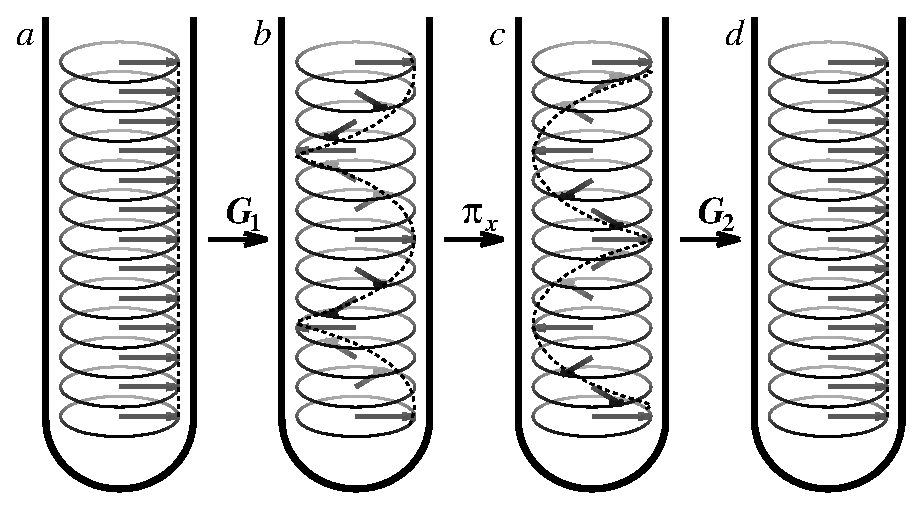
\epsfig{file=gradecho.eps,width=4in}
\end{center}
\caption[Écho de spin avec gradient]{Écho de spin avec gradient.
$a$. Aimantation transversale initiale. 
$b$. effet de la première impulsion de gradient. 
$c$. Inversion de l'aimantation.
$d$. effet de la seconde impulsion de gradient.}
\label{fig:gradecho}
\end{figure}

\section{Matrice densité et modèle vectoriel}
La présentation du modèle vectoriel pour les systèmes de spins isolés est l'objet
du chapitre \ref{chap:bloch}.

De la même manière qu'un système à un spin est caractérisé par une unique
fréquence de résonance et est classiquement décrit par un seul vecteur aimantation,
un système de deux spins faiblement couplés est caractérisé par quatre fréquences
de résonance et est décrit, dans le cadre du modèle vectoriel, par quatre vecteurs.

Les quatre états de spin $\al\al$, $\be\al$, $\al\be$ et $\be\be$ sont liés par quatre
transitions à $\pm 1$ quanta, comme indiqué sur la figure \ref{fig:diagramisj}.
Deux vecteurs aimantation seront associés aux transitions du noyau $I$
et deux au noyau $S$.
L'aimantation d'équilibre du noyau $I$ résulte de la somme des différences de populations :
\begin{equation}
\Delta P(I) = (p_{\al\al} - p_{\be\al}) + (p_{\al\be} - p_{\be\be})
\end{equation}
Le modèle vectoriel considère l'évolution des deux composantes de l'aimantation dues
aux noyaux $I$ d'une part et de des deux composantes dues aux noyaux $S$ d'autre part.
Pour chaque noyau, une composante diffère de l'autre par l'état $\al$ ou $\be$
de l'autre noyau.
La composante notée $\aimvec_{I\al}$ correspond à la paire d'états
($\al\al$, $\be\al$) liée à la transition du noyau $I$ quand le noyau $S$ 
se trouve dans l'état $\al$.
La fréquence de cette transition est $\nu_1 = \nu_I - J/2$.
La composante transversale du vecteur $\aimvec_{I\al}$ est sujette à un mouvement
de précession de fréquence $\nu_1$ dans le référentiel du laboratoire.
Le système $IS$ est décrit par l'ensemble des quatre
vecteurs $\aimvec_{I\al}$, $\aimvec_{I\be}$,
$\aimvec_{\al S}$ et $\aimvec_{\be S}$. 

La matrice densité d'un système de 2 spins évolue dans un espace de dimension 16, alors
qu'un ensemble de 4 vecteurs dans un espace physique de dimension 3 ne fait intervenir
que 12 coordonnées.
Les 4 (16 $-$ 12) coordonnées manquantes sont celles qui décrivent les 4 cohérences à
0 et $\pm$ 2 quanta du système.
Tant que l'on ne cherche pas à mettre en {\oe}uvre des expériences fondées sur des évolutions
autres que celles des populations et des cohérences d'ordre $\pm 1$,
le modèle vectoriel est susceptible de fournir une
interprétation graphique correcte des observations.

Du point de vue du formalisme des opérateurs, les trois coordonnées du
vecteur $\aimvec_{I\al}$ sont fournies par les coefficients multiplicatifs
des opérateurs $I_xS_{\al}$, $I_yS_{\al}$ et $I_zS_{\al}$, la matrice densité
étant exprimée dans ce qui pourrait être une base
\{
$I_xS_{\al}$, $I_yS_{\al}$, $I_zS_{\al}$,
$I_xS_{\be}$, $I_yS_{\be}$, $I_zS_{\be}$,
$I_{\al}S_x$, $I_{\al}S_y$, $I_{\al}S_z$,
$I_{\be}S_x$, $I_{\be}S_y$, $I_{\be}S_z$
\}
du sous-espace des états susceptibles d'être décrits par le formalisme vectoriel.
Ce n'est pas une base car
\begin{eqnarray}
\label{eqn:izsza}
2I_zS_z & = & I_z(S_{\al}-S_{\be}) = I_zS_{\al} - I_zS_{\be} \\
\label{eqn:izszb}
2I_zS_z & = & (I_{\al}-I_{\be})S_z = I_{\al}S_z - I_{\be}S_z
\end{eqnarray}
et en sachant qu'un même état ne peut être décrit de deux manières différentes
comme combinaisons linéaires des mêmes états de base.
Toutefois, cet ensemble de 12 éléments contient 8 états d'ordre de cohérence $\pm 1$
qui constituent une base.
Le modèle vectoriel est donc particulièrement adapté au suivi de l'évolution
de l'aimantation transversale.
L'extension aux opérateurs de population est néanmoins acceptable,
sous réserve de ne pas être trop sourcilleux sur la rigueur mathématique.

L'état initial du système, en omettant la partie proportionnelle
à la matrice identité, s'écrit :
\begin{eqnarray}
\sigma_0 & = & \Delta P(I)/2 \cdot I_z + \Delta P(S)/2 \cdot S_z\\
& = & \frac{1}{2}\left(
\Delta P(I)(I_zS_{\al} + I_zS_{\be}) 
+ \Delta P(S)(I_{\al}S_z + I_{\be}S_z) 
\right)
\end{eqnarray}
ce qui correspond graphiquement à la figure \ref{fig:vectisinit}
où la superposition des paires de vecteurs identiques est remplacée
par une flèche double.
La partie gauche de la figure se rapporte au noyau $I$ et
les annotations $\al$ et $\be$ décrivent l'état de spin du noyau $S$.

\begin{figure}[hbt]
\begin{center}
\begin{pspicture}(-3,-2)(3,3)
\SpecialCoor
\psline{->}(0.5;150)(2.5;-30)
\psline{->}(0.5;270)(2.5;90)
\psline{->}(0.5;30)(2.5;210)
\psline[linewidth=0.06,doubleline=true,doublesep=0.05]{->}(0,0)(2;90)
\uput[210](2.5;210){$X$}
\uput[-30](2.5;-30){$Y$}
\uput[90](2.5;90){$Z$}
\rput(-0.5,0){$O$}
\rput(2;90){\rput(-0.25,0){$\alpha$}\rput(0.25,0){$\beta$}}
\rput(0,-1.75){I}
\end{pspicture}
\begin{pspicture}(-3,-2)(3,3)
\SpecialCoor
\psline{->}(0.5;150)(2.5;-30)
\psline{->}(0.5;270)(2.5;90)
\psline{->}(0.5;30)(2.5;210)
\psline[linewidth=0.06,doubleline=true,doublesep=0.05]{->}(0,0)(1;90)
\uput[210](2.5;210){$X$}
\uput[-30](2.5;-30){$Y$}
\uput[90](2.5;90){$Z$}
\rput(-0.5,0){$O$}
\rput(1;90){\rput(-0.25,0){$\alpha$}\rput(0.25,0){$\beta$}}
\rput(0,-1.75){S}
\end{pspicture}

\caption{\label{fig:vectisinit}
\small Représentation vectorielle de l'état initial d'un système $IS$}
\end{center}
\end{figure}

Une impulsion de RF $\pi/2_y$ appliquée à la fréquence de $I$ amène l'aimantation
sur l'axe $OX$ du référentiel tournant lié à $I$.
En d'autres termes :
\begin{equation}
I_zS_{\al} \flham{\pi/2_y} I_xS_{\al}
\qetq
I_zS_{\be} \flham{\pi/2_y} I_xS_{\be}
\end{equation}

Les vecteurs $\aimvec_{I\al}$ et $\aimvec_{I\be}$, superposés sur l'axe $OX$
juste après l'impulsion, vont ensuite évoluer à leur pulsation de précession propres
$\Omega_{I\alpha} = \omsi - \pi J$ et 
$\Omega_{I\beta} = \omsi + \pi J$ dans le référentiel tournant,
comme sur la figure \ref{fig:vectisevol} limitée à la représentation
du plan transversal $XOY$.
Après un temps $t$ dévolution libre du système sous l'action de 
l'hamiltonien $H$, $\aimvec_{I\alpha}$ et $\aimvec_{I\beta}$ tournent
respectivement des angles $\theta_{\alpha} = \Omega_{I\alpha} t$ et
$\theta_{\beta} = \Omega_{I\beta} t$.
L'angle entre les deux vecteurs est $2\pi J t$.

\begin{figure}[hbt]
\begin{center}
\begin{pspicture}(-6,-2)(6,2)
\SpecialCoor
\rput(-4,0){
\pscircle(0,0){1.5}
\psline{->}(2;180)(2;0)
\psline{->}(2;-90)(2;90)
\uput[0](2;0){$X$}
\uput[90](2;90){$Y$}
\psline[linewidth=0.06,doubleline=true,doublesep=0.05]{->}(0,0)(1.5;0)
\uput[0](1.5;0){\rput(0,-0.25){$\alpha$}\rput(0,0.25){$\beta$}}
}
\rput(4,0){
\pscircle(0,0){1.5}
\psline{->}(2;180)(2;0)
\psline{->}(2;-90)(2;90)
\uput[0](2;0){$X$}
\uput[90](2;90){$Y$}
\psline[linewidth=0.06]{->}(0,0)(1.5;150)
\psline[linewidth=0.06]{->}(0,0)(1.5;80)
\uput[80](1.5;80){$\alpha$}
\uput[150](1.5;150){$\beta$}
\psarc[arcsepB=0.06,linewidth=0.02]{->}(0,0){0.9}{0}{80}
\psarc[arcsepB=0.06,linewidth=0.02]{->}(0,0){1.0}{0}{150}
\uput[220](1.1;40){$\theta_{\alpha}$}
\uput[120](0.8;120){$\theta_{\beta}$}
}
\psline[linewidth=0.04]{->}(-0.75,0)(0.75,0)
\rput(0,0.25){$Ht$}
\end{pspicture}
\caption{\label{fig:vectisevol}
\small Evolution de l'aimantation transversale du noyau $I$ d'un syst\`eme $IS$}
\end{center}
\end{figure}

La détection des deux composantes de l'aimantation de $I$ conduit après TF 
à un doublet de lorentziennes en phase
de fréquences séparées de la constante de couplage $J$ et centrées sur $\nu_I$.
Le même raisonnement peut être effectué indépendemment (système $IS$ hétéronucléaire)
ou simultanément (système $IS$ homonucléaire) pour le noyau S.

Le modèle vectoriel aide à visualiser
simplement l'action d'un écho de spin de durée $2T$ sur l'aimantation transversale 
du noyau $I$ d'un système $IS$ hétéronucléaire,
et ceci dans les trois situations possibles (figure \ref{fig:vectecho}) :

\begin{figure}[hbt]
\begin{center}
\begin{pspicture}(-6,-3)(6,3)
\SpecialCoor
\psset{labelsep=2pt}
\rput(-3.75,0){
\rput(-1.75,0){
\pscircle(0,0){0.75}
\psline[linewidth=0.04,doubleline=true,doublesep=0.03]{->}(0,0)(0.75;0)
\uput[-10](0.75;-10){$\alpha$}
\uput[10](0.75;10){$\beta$}
}
\rput(1.75,0){
\pscircle(0,0){0.75}
\psline[linewidth=0.04]{->}(0,0)(0.75;50)
\uput[50](0.75;50){$\alpha$}
\psline[linewidth=0.04]{->}(0,0)(0.75;70)
\uput[70](0.75;70){$\beta$}
}
\psline[linewidth=0.03]{->}(-0.5,0)(0.5,0)
\rput(0,0.25){$HT$}
}
\rput(-0.75,0){
\psline[linewidth=0.03]{->}(0,0)(1.5,0)
\psline[linewidth=0.03]{->}(0.25,0)(0.5,2.25)(1.5,2.25)
\psline[linewidth=0.03]{->}(0.25,0)(0.5,-2.25)(1.5,-2.25)
\rput(1,2.5){$\pi_x(I)$}
\rput(1,0.25){$\pi_x(S)$}
\rput(1,-2){$\pi_x(I)$}
\rput(1,-2.5){$\pi_x(S)$}
}
\rput(3.75,0){
\rput(0,2.25){
\rput(-1.75,0){
\pscircle(0,0){0.75}
\psline[linewidth=0.04]{->}(0,0)(0.75;-50)
\uput[-50](0.75;-50){$\alpha$}
\psline[linewidth=0.04]{->}(0,0)(0.75;-70)
\uput[-70](0.75;-70){$\beta$}
}
\rput(1.75,0){
\pscircle(0,0){0.75}
\psline[linewidth=0.04,doubleline=true,doublesep=0.03]{->}(0,0)(0.75;0)
\uput[-10](0.75;-10){$\alpha$}
\uput[10](0.75;10){$\beta$}
}
\psline[linewidth=0.03]{->}(-0.5,0)(0.5,0)
\rput(0,0.25){$HT$}
}
\rput(0,0){
\rput(-1.75,0){
\pscircle(0,0){0.75}
\psline[linewidth=0.04]{->}(0,0)(0.75;50)
\uput[50](0.75;50){$\beta$}
\psline[linewidth=0.04]{->}(0,0)(0.75;70)
\uput[70](0.75;70){$\alpha$}
}
\rput(1.75,0){
\pscircle(0,0){0.75}
\psline[linewidth=0.04,doubleline=true,doublesep=0.03]{->}(0,0)(0.75;120)
\uput[110](0.75;110){$\beta$}
\uput[130](0.75;130){$\alpha$}
}
\psline[linewidth=0.03]{->}(-0.5,0)(0.5,0)
\rput(0,0.25){$HT$}
}
\rput(0,-2.25){
\rput(-1.75,0){
\pscircle(0,0){0.75}
\psline[linewidth=0.04]{->}(0,0)(0.75;-50)
\uput[-50](0.75;-50){$\beta$}
\psline[linewidth=0.04]{->}(0,0)(0.75;-70)
\uput[-70](0.75;-70){$\alpha$}
}
\rput(1.75,0){
\pscircle(0,0){0.75}
\psline[linewidth=0.04]{->}(0,0)(0.75;20)
\uput[20](0.75;20){$\beta$}
\psline[linewidth=0.04]{->}(0,0)(0.75;-20)
\uput[-20](0.75;-20){$\alpha$}
}
\psline[linewidth=0.03]{->}(-0.5,0)(0.5,0)
\rput(0,0.25){$HT$}
}
}
\end{pspicture}
\caption{\label{fig:vectecho}
\small Évolution de l'aimantation transversale du noyau $I$ d'un système $IS$ pendant un
écho de spin.}
\end{center}
\end{figure}

\begin{enumerate}
\item Seul $I$ subit une impulsion RF $\pi_x$. Pendant la deuxième partie de l'écho
chaque composante décrit exactement le même angle que pendant la première partie.
Elle se retrouvent à leur emplacement initial quel que soit $\omsi$ et $J$.
Les effets du couplage et de l'offset de $I$ sont refocalisés.
\item Seul $S$ subit une impulsion RF $\pi_x$. L'impulsion sur $S$ permute les
"étiquettes" $\al$ et $\be$ :
\begin{equation}
S_{\al} \flham{\pi_x(S)} S_{\be}
\qetq
S_{\be} \flham{\pi_x(S)} S_{\al}
\end{equation}
avec pour conséquence que chaque composante à tourné à la pulsation
$\omsi + \pi J$ pendant $T$ et $\omsi - \pi J$ aussi pendant $T$.
Les composantes se superposent au temps $2T$ comme si elles avaient tourné
à la pulsation $\omsi$.
L'effet du couplage est refocalisé.
\item $I$ et $S$ subissent une impulsion RF $\pi_x$.
Le vecteur $\aimvec_{I\al}$ a tourné à la pulsation $\omsi - \pi J$ pendant
la première période, est devenu $\aimvec_{I\be}$ par action de l'impulsion
$\pi_x(S)$ et a tourné à la pulsation $\omsi + \pi J$ pendant
la seconde période. 
Tout se passe comme si seul le couplage avait agit pendant $2T$.
L'effet de l'offset de $I$ (et de $S$, par symétrie) est refocalisé.
\end{enumerate}

Le lecteur pourra constater qu'utiliser une impulsion $\pi_y$ transforme les
vecteurs finaux en leur opposé, en plein accord avec la description
de l'écho de spin utilisant la matrice densité.
Ce tableau du modèle vectoriel sera complété lors de l'étude du transfert
d'aimantation cohérent.

L'extension du modèle à un système $ISL$ faiblement couplé fait apparaître
pour chaque noyau quatre composantes.
Ainsi, celles du noyau$ $I seront notées $\aimvec_{I\al\al}$,
$\aimvec_{I\be\al}$, $\aimvec_{I\al\be}$ et $\aimvec_{\be\be}$.
Les principes exposés aux paragraphes précédents s'appliquent
de manière immédiate.

\chapter[RMN 1D]{Expériences à une dimension}

La plus simple des expériences à une dimension (1D) est celle où après
une période de mise ou de remise en équilibre de l'échantillon, 
l'excitation des systèmes de spins par une unique impulsion 
de radiofréquence est suivie de la détection du signal de précession libre.
Le terme "1D" est relatif au fait que le spectre obtenu après TF
est une fonction d'une seule variable fréquencielle.
Des expériences 1D plus complexes font intervenir la relaxation,
divers types de transfert d'aimantation, la spectroscopie à plusieurs quanta
ou le découplage pour améliorer ou compléter les informations contenues dans
les spectres "élémentaires".
Les mesures des temps de relaxation et d'effet Overhauser nucléaire précisent 
la nature de l'environnement des noyaux à travers l'espace.
Les liaisons chimiques sont le support du couplage scalaire et autorisent
l'analyse des systèmes de spin grâce aux transferts d'aimantation. 
Enfin, le découplage est une méthode expérimentale indispensable
en RMN hétéronucléaire car elle apporte à la fois une simplification
des spectres et une amélioration de la sensibilité.
Des applications de ces concepts à la spectroscopie 1D hétéronucléaire
et aux expériences homonucléaires sélectives 1D seront présentées ci-après.

\section{Effet Overhauser Nucléaire, nOe}
\label{sec:noe}
Le problème le plus critique posé par l'enregistrement de spectres 
de noyaux isotopiquement dilués et de faible rapport gyromagnétique 
est l'obtention d'un rapport signal sur bruit suffisant pour permettre
une l'exploitation analytique des données.
C'est par exemple le cas des noyaux de \carb.

L'effet Overhauser nucléaire se manifeste par une modification des 
intensités de certaines résonances lorsque d'autres sont saturées.
Cet effet se manifeste entre noyaux de nature semblable ou différente,
ainsi qu'entre noyaux et électrons (effet Overhauser électronique),
pour peu qu'un couplage dipolaire existe entre les spins des particules.

Le couplage dipolaire est l'interaction directe qui s'exerce à travers
l'espace entre deux particules qui possèdent un moment magnétique.
En considérant ces deux particules dans un état quantique défini par
les deux valeurs de $m_s$, l'énergie de l'interaction dépend de l'orientation
de la droite qui joint les particules avec la direction de $\bzerovec$.
Au cours du temps, la réorientation aléatoire des molécules
au sein d'un liquide isotrope produit une interaction 
dont l'intensité est nulle en moyenne. 
Le couplage dipolaire est ainsi indétectable si on ne considère que
les fréquences de résonance des noyaux.
Toutefois, l'existence d'une interaction d'intensité aléatoire
entre noyaux contribue à la relaxation de leur aimantation macroscopique
(il faut, à ce niveau de l'exposé, l'admettre).
De fait, toute perturbation aléatoire des niveaux énergétiques des noyaux
contribue à la relaxation.
L'existence du couplage dipolaire a pour conséquence que la relaxation
longitudinale de chaque noyau est influencée par celle de l'autre noyau.

Considérons deux noyaux $I$ et $S$ de rapports gyromagnétiques $\gi$ et $\gs$.
Les différences de population $\Delta P(I)$ et $\Delta P(S)$ sont
aussi appelées polarisations et notées $\poli$ et $\pols$, dont les
valeurs d'équilibre sont $\poliz$ et $\polsz$.
L'évolution des polarisations est donnée par les équations de Solomon :
\begin{eqnarray}
\label{eqn:soli}
\derivt{\poli} & = & -\rho_I \dpoli -\sigma \dpols \\
\label{eqn:sols}
\derivt{\pols} & = & -\rho_S \dpols -\sigma \dpoli
\end{eqnarray}
qui constituent une généralisation de l'équation $\ref{eqn:t1}$
relative à la relaxation longitudinale.

La grandeur $\sigma$ caractérise la vitesse (en $s^{-1}$) de relaxation \emph{croisée}
entre les noyaux $I$ et $S$.
Dans le cas où $\sigma$ est nul, les aimantations de $I$ et $S$ évoluent indépendamment.
Ainsi
\begin{equation}
\frac{1}{T_1(I)} = \rho_I^{\dipolaire} + \rho_I^{\autres}
\end{equation}
En effet, la  relaxation longitudinale de $I$ est en partie causée par son interaction
dipolaire avec $S$, mais aussi par d'autres influences de nature aléatoire.

La saturation de l'aimantation du noyau $S$ par un champ de radiofréquence continu
(voir section \ref{sec:eqnbloch}) d'intensité suffisante conduit à $\pols = 0$
et donc à une évolution des polarisations jusqu'à un nouvel état stationnaire
différent de l'état d'équilibre.
A l'état stationnaire, l'équation \ref{eqn:soli} conduit à
\begin{eqnarray}
0 & = & -\rho_I \dpoli + \sigma \polsz \\
\frac{\dpoli}{\poliz} & = & \frac{\sigma}{\rho_I} \frac{\polsz}{\poliz}
\end{eqnarray}
Sachant d'après l'équation \ref{eqn:diffpopgamma} que les polarisations 
d'équilibre sont proportionnelles
aux rapports gyromagnétiques, le rapport d'effet Overhauser $\eta$ s'écrit :
\begin{equation}
\eta = \frac{\dpoli}{\poliz} = \frac{\gs}{\gi} \frac{\sigma}{\rho_I}
\end{equation}
Il caractérise l'augmentation relative d'intensité du signal de $I$ lorsque l'aimantation
des noyaux $S$ est préalablement saturée puisque pour un noyau donné,
l'intensité des signaux mesurés est proportionnelle aux différences de population.
Dans les situations où le couplage dipolaire est le mécanisme de relaxation prépondérant
et que les molécules se réorientent très rapidement (petites molécules en solution
de faible viscosité), le rapport $\sigma/\rho_I$ vaut $1/2$, et donc
\begin{equation}
\label{eqn:noe}
\frac{\aimzI}{\aimzzi} = 1+\eta = 1+\frac{1}{2}\frac{\gs}{\gi}
\end{equation}

\section{Découplage}
Considérons un système hétéronucléaire de deux noyaux $I$ et $S$ couplés scalairement.
L'évolution d'un état $I_{x,y}$ conduit, pendant la détection de l'aimantation de $I$, à
deux raies de résonance aux fréquences $\omsi \pm \pi J$ et d'intensité moitié par
rapport à un noyau non couplé.

Si les noyaux $S$ subissent en permanence une série d'échos de spin, 
l'hamiltonien effectif d'évolution, $\omsi I_z$, ne fait pas intervenir la constante
de couplage. 
L'aimantation de $I$ évolue alors comme si $I$ n'était pas couplé à $S$.
L'évolution libre d'un terme $2I_{x,y}S_z$ ne peut alors pas conduire
à tes termes $I_{x,y}$ et n'est donc pas susceptible de produire un signal.

Dans la pratique, la série d'échos de spin pourrait être constituée d'une 
série d'impulsions à 180 degrés sans délai intercalé. 
Sous cette forme, découpler serait équivalent à envoyer
un champ de radiofréquence continu. Si on désire que le découplage soit uniforme
pour l'ensemble des noyaux $I$ dont la fréquence de résonance s'étend
sur plusieurs (ou dizaines de) kHz, cela implique des valeurs de champ 
$\bunmax$ incompatibles avec les contraintes matérielles liées à la sonde 
ou à l'échantillon (ou aux deux) par suite soit de l'effet Joule
soit des pertes diélectriques.
Les séquences utilisées pour le découplage \emph{large bande}
sont constituée d'impulsions modulées en phase, en durée, voire en amplitude,
le plus souvent optimisées par calcul numérique.

Notons qu'une telle séquence, appliquée sur l'aimantation d'équilibre de $S$
conduit aussi à la saturation de cette aimantation.

\section{RMN du \carb}
L'enregistrement d'un spectre de RMN du \carb (noyaux $I$), 
dans sa forme la plus simple, requiert la saturation de l'aimantation des \prot
(noyaux $S$) et l'obtention d'un état stationnaire pour l'aimantation des noyaux $I$,
l'excitation de l'aimantation des noyaux de \carb, puis la détection du signal
avec application d'une séquence de découplage sur les noyaux \prot.
En résumé, il s'agit d'une séquence relaxation -- impulsion -- acquisition analogue
à celle étudiée jusqu'ici sauf que les noyaux non observés sont soumis en permanence
à une séquence de découplage.

Sauf superposition accidentelle ou liée à la symétrie des molécules étudiés, chaque
atome de carbone fournit une résonance identifiable par le déplacement chimique associé.
L'information de couplage avec les noyaux \prot est perdue, mais en contrepartie
les enchevêtrements de multiplets qui rendent les spectres peu lisibles sont éliminés.
L'intensité des signaux des \carb liés à des \prot est multipliée par un facteur pouvant aller
jusqu'à 3 ($\gs/\gi = 4$ dans l'équation \ref{eqn:noe}).
Les signaux des carbones quaternaires ne profitent évidemment pas (ou peu) de l'effet Overhauser.
De plus, leur temps de relaxation peut valoir plusieurs secondes car ils ne sont
que faiblement soumis à la relaxation dipolaire.
Le temps qu'il faudrait attendre entre deux impulsions (temps de répétition $T_R$)
pour que l'aimantation de $I$
revienne près de sa valeur initiale rend peu efficace l'augmentation du rapport 
signal sur bruit par accumulation de plusieurs \FID.
Cela conduit à utiliser un angle de nutation de l'aimantation optimisé par rapport 
à $T_R$ et à $T_1$, angle qui peut être très inférieur à $\pi/2$ et
qui dépend de $T_1$, grandeur qui est inconnue le plus souvent.
La saturation partielle des signaux de \carb et l'inégalité des noyaux devant
l'effet Overhauser rend hasardeuses les tentatives de tirer une information quantitative
des spectres enregistrées dans des conditions inappropriées.

L'enregistrement de spectres de RMN du \carb dans des conditions quantitatives
requiert de n'actionner le découplage que pendant l'acquisition du signal
et d'utiliser le $T_R$ le plus long possible compatible avec le rapport signal sur bruit
désiré et le temps total de mesure disponible.

L'augmentation de l'intensité des signaux des noyaux $S$ peut aussi être réalisée
sans recourir à l'effet Overhauser, comme indiqué ci-après.

\section{Transfert hétéronucléaire d'aimantation}
Dans la suite du texte, et contrairement à ce qui est écrit depuis le début
de ce chapitre, les noyaux \prot seront notés $I$ et les hétéronoyaux $S$,
indépendemment de la nature du noyau détecté.
Dans l'étude de l'effet Overhauser, il est d'usage d'appeler $S$
le noyau dont l'aimantation est \emph{s}aturée.

\begin{figure}[hbt]
\begin{center}
\begin{pspicture}(0,0)(6,5.5)
% sequence I
\psline(1,3.5)(6,3.5)
\rput(0.5,4){RF($I$)}
\psline[linewidth=2mm]{-}(1.9,3.5)(1.9,4.5)
\rput(1.9,4.7){$\pi/2_x$}
\psline[linewidth=2mm]{-}(3.9,3.5)(3.9,4.5)
\rput(3.9,4.7){$\pi/2_y$}
\rput(2.9,4){$T$}
% sequence S
\psline(1,2)(6,2)
\rput(0.5,2.5){RF($S$)}
\psline[linewidth=2mm]{-}(4.1,2)(4.1,3)
\rput(4.3,3.2){$\pi/2_x$}
% time marks
\psline{->}(1,1)(6,1)
\psline[linewidth=0.25mm,linestyle=dashed]{-}(1.8,3.3)(1.8,0.8)
\rput(1.7,0.5){0}
\psline[linewidth=0.25mm,linestyle=dashed]{-}(2,3.3)(2,0.8)
\rput(2.1,0.5){1}
\psline[linewidth=0.25mm,linestyle=dashed]{-}(3.8,3.3)(3.8,0.8)
\rput(3.7,0.5){2}
\psline[linewidth=0.25mm,linestyle=dashed]{-}(4,1.8)(4,0.8)
\rput(4,0.5){3}
\psline[linewidth=0.25mm,linestyle=dashed]{-}(4.2,1.3)(4.2,0.8)
\rput(4.3,0.5){4}
\psline[linewidth=0.25mm,linestyle=dashed]{-}(5,1.6)(5,0.8)
\rput(5,0.5){$t$}
% FID
\rput(4.2,2){
\pscurve(0,0.5)(0.5,0.25)(1.5,0)
\pscurve(0,-0.5)(0.5,-0.25)(1.5,0)
\psline(0,0.5)(0,-0.5)
}
\end{pspicture}
\caption{\label{fig:transmagheta}
Principe du transfert d'aimantation hétéronucléaire.}
\end{center}
\end{figure}

\subsection{Principe}

Détaillons l'effet de la séquence \ref{fig:transmagheta}
sur la matrice densité initiale $I_z + aS_z$ d'un système scalairement 
couplé $IS$ où $a = \gs/\gi$, soit $a = $ 0,25 si $S$ 
désigne les noyaux de \carb. 
Le temps $T$ vaut $1/2J$. 
Calculons l'évolution de $I_z$ aux instants 1 à 4 en faisant l'hypothèse
simplificatrice $\omsi = 0$ :
\begin{eqnarray}
\sigma_1 & = & - I_y \\
\sigma_2 & = & -\cos\left(\frac{\pi J}{2 J}\right)\cdot I_y + 
\sin\left(\frac{\pi J}{2 J}\right) \cdot 2I_xS_z = 2I_xS_z \\
\sigma_3 & = & -2I_zS_z \\
\label{eqn:fintransmag}
\sigma_4 & = & 2I_zS_y
\end{eqnarray}

\begin{figure}[hbt]
\begin{center}
\begin{pspicture}(0,-3)(10,2.5)
% a
\psline(0,0)(2,0)
\pstriangle*(0.5,0)(0.2,-0.5)
\pstriangle*(1.5,0)(0.2,-0.5)
\rput(0.5,-1){-1/4}
\rput(1.5,-1){-1/4}
\rput(0,-2){$a$}
% b
\psline(4,0)(6,0)
\pstriangle*(4.5,0)(0.2,2)
\pstriangle*(5.5,0)(0.2,-2)
\rput(4.5,2.5){1}
\rput(5.5,-2.5){-1}
\rput(4,-2){$b$}
% c
\psline(8,0)(10,0)
\pstriangle*(8.5,0)(0.2,1.5)
\pstriangle*(9.5,0)(0.2,-2.5)
\rput(8.5,2){3/4}
\rput(9.5,-3){-5/4}
\rput(8,-2){$c$}
% deco
\rput(3,0){+}
\rput(7,0){=}
\end{pspicture}
\caption{\label{fig:picsinept}
Intensités des pics obtenues par la séquence de la Figure \ref{fig:transmagheta}.
$a$. contribution des noyaux $S$, $b$. contribution des noyaux $I$, $c$ résultat.}
\end{center}
\end{figure}

Le spectre correspondant à l'évolution libre de $\sigma_4$ est un 
doublet antiphase en dispersion d'intensité relative 1. 
Le second terme de l'état initial, $a S_z$, commute avec tous les opérateurs 
qui interviennent entre les instants 0 et 3 et reste donc inchangé jusque là. 
L'impulsion $\pi/2$ sur $S$ le transforme en $-aS_y$ qui évolue ensuite pour 
donner un doublet en phase et en dispersion d'intensité relative $-a$.
Le spectre réellement observé, après correction de la phase 
(présentation des raies en absorption) consiste en une paire de raies 
d'intensités relatives $(1-a)$ et $(-1-a)$ soit 3/4 et -5/4 si a = 0,25
(Figure \ref{fig:picsinept}). 
En comparaison les intensités relatives des composantes du doublet qui 
aurait été obtenu par la séquence impulsion-détection, 
sans effect Overhauser ni découplage, valent $a$ et $a$. 

L'étape-clé du transfert d'aimantation est la transformation 
subie par le système sous l'action simultanée 
(si on considère des impulsions de durée pratiquement nulle)
des deux impulsions d'angle $\pi/2$ sur un état couplé du noyau $I$
qui produit un état couplé du noyau $S$.
L'intensité du signal de pulsation $\omss$ qui provient du 
transfert d'aimantation est proportionnelle à l'aimantation initiale 
du noyau $I$, plus importante que celle de $S$.

Il doit nécessairement y avoir entre les phases des deux impulsions 
appliquées aux noyaux $I$ un écart de $\pi/2$.
Si la phase de la seconde impulsion était nulle :
\begin{eqnarray}
\sigma_2 & = & 2I_xS_z \\
\sigma_3 & = & 2I_xS_z \quad \mbox{car $\sigma_2$ et $I_x$ commutent} \\
\sigma_4 & = & -2I_xS_y
\end{eqnarray}
Cet état à 0 et 2 quanta évolue sans donner de signal, ce qui n'est
pas le but recherché ici.

Dans l'expérience décrite par la figure \ref{fig:transmagheta}, 
le temps $T$ a été choisi égal à $1/2J$ pour que l'état non couplé
$\sigma_1$ n'évolue seulement que vers un état couplé. 
Dans la réalité il n'y a pas une valeur unique de $J$ mais une certaine dispersion
autour d'une valeur moyenne (environ 145 Hz, si $S$ est un noyau de \carb).
Dans le cas général $\sigma_2 = -\cos(\pi J T)I_y + \sin(\pi J T)2I_xS_z$.
Le second terme conduit au signal souhaité, mais son intensité dépend de $\sin(\pi J T)$,
qui vaut $\pm 1$ lorsque $\pi J T$ vaut $(2n+1)\pi/2$, c'est à dire lorsque $T$
est un multiple impair de $1/2J$. 
Le terme proportionnel à $I_y$ reste inchangé sous l'action de l'impulsion 
$\pi/2_y(I)$; il ne contribue donc pas au signal enregistré aux fréquences du noyau $S$.

\subsection{Lien avec le modèle vectoriel}

\begin{figure}[hbt]
\begin{center}
\begin{pspicture}(-6,-5)(6,5)
\SpecialCoor
\rput(-3,2.5){
\psline{->}(0.5;150)(2.5;-30)
\psline{->}(0.5;270)(2.5;90)
\psline{->}(0.5;30)(2.5;210)
\uput[210](2.5;210){$X$}
\uput[-30](2.5;-30){$Y$}
\uput[90](2.5;90){$Z$}
\psline[linewidth=0.08,doubleline=true,doublesep=0.05]{->}(0,0)(2;90)
\uput[90](1.8;80){$\alpha$}
\uput[90](1.8;100){$\beta$}
\rput(-0.5,0){$O$}
}
\rput(0,2.5){
\psline{->}(-1,0)(1,0)
\rput(0,0.25){$\pi/2_x(I)$}
}
\rput(3,2.5){
\psline{->}(0.5;150)(2.5;-30)
\psline{->}(0.5;270)(2.5;90)
\psline{->}(0.5;30)(2.5;210)
\uput[210](2.5;210){$X$}
\uput[-30](2.5;-30){$Y$}
\uput[90](2.5;90){$Z$}
\psline[linewidth=0.08,doubleline=true,doublesep=0.05]{->}(0,0)(2;150)
\uput[150](1.8;140){$\alpha$}
\uput[150](1.8;160){$\beta$}
\rput(0.5,0){$O$}
}
\rput(6,2.5){
\psline{->}(-1,0)(1,0)
\rput(0,0.25){$T = 1/2J$}
}
\rput(-3,-2.5){
\psline{->}(0.5;150)(2.5;-30)
\psline{->}(0.5;270)(2.5;90)
\psline{->}(0.5;30)(2.5;210)
\uput[210](2.5;210){$X$}
\uput[-30](2.5;-30){$Y$}
\uput[90](2.5;90){$Z$}
\psline[linewidth=0.08]{->}(0,0)(2;210)
\uput[210](1.8;200){$\alpha$}
\psline[linewidth=0.08]{->}(0,0)(2;30)
\uput[30](1.8;20){$\beta$}
\rput(-0.5,0){$O$}
}
\rput(0,-2.5){
\psline{->}(-1,0)(1,0)
\rput(0,0.25){$\pi/2_y(I)$}
}
\rput(3,-2.5){
\psline{->}(0.5;150)(2.5;-30)
\psline{->}(0.5;270)(2.5;90)
\psline{->}(0.5;30)(2.5;210)
\uput[210](2.5;210){$X$}
\uput[-30](2.5;-30){$Y$}
\uput[90](2.5;90){$Z$}
\psline[linewidth=0.08]{->}(0,0)(2;90)
\uput[90](1.8;80){$\alpha$}
\psline[linewidth=0.08]{->}(0,0)(2;-90)
\uput[-90](1.8;-80){$\beta$}
\rput(-0.5,0){$O$}
}
\end{pspicture}

\caption{\label{fig:transmagvec}
\small Transfert d'aimantation selon le modèle vectoriel}
\end{center}
\end{figure}

L'évolution de l'aimantation initiale des noyaux $I$ entre les
instants 0 et 3 est retracée par la figure \ref{fig:transmagvec}.
L'évolution pendant $T$ correspond à une rotation de 
$\pm J/2 \cdot 1/2J = \pm1/4$ de tour, soit un angle de $\pm \pi/2$.
La représentation vectorielle de l'état $2I_zS_z$ est constitée d'une paire
de vecteurs opposés (donc de somme nulle).
Le terme de l'état inital $\poli/2 \cdot I_z$ contribue aux populations
($p_{\al\al}$, $p_{\al\be}$, $p_{\be\al}$, $p_{\be\be}$) pour 
($\poli/4$, $\poli/4$, $-\poli/4$, $-\poli/4$) selon les équations
\ref{eqn:popisa} à \ref{eqn:popisd}.
L'état $\poli/2 \cdot 2I_zS_z$ contribue, d'après les mêmes équations
pour ($\poli/4$, -$\poli/4$, $-\poli/4$, $\poli/4$) 
aux populations des 4 états du système.
Cela revient à dire que la séquence $\pi/2_x(I)$ -- $1/2J$ -- $\pi/2_y(I)$
a inversé sélectivement les populations
des états $\al\be$ et $\be\be$, ce correspond bien a l'inversion
de la partie de l'aimantation de $I$ qui est étiquetée $\be$ en
ce qui concerne l'état du noyau $S$.
Après l'instant 3, l'intensité de la résonance de $S$ étiquetée $\al$
est proportionnelle à $p_{\al\al}$ - $p_{\al\be} = \poli/2$.
L'intensité de celle étiquetée $\be$ est $p_{\be\al}$ - $p_{\be\be} = -\poli/2$.
En résumé, l'aimantation initiale de $I$ devient à l'instant 3 la source
d'un doublet antiphase pour $S$, d'intensité totale certes nulle, mais dont
chacune des composantes est plus intense (d'un facteur $\gi/\gs$) que
les composantes en phase issues de l'aimantation initiale du noyau $S$.
L'origine du transfert d'aimantation via l'état $2I_zS_z$
peut être vue dans l'identité des membres de droite des équations
\ref{eqn:izsza} et \ref{eqn:izszb}, identité qui permet de transférer les vecteurs
opposés obtenus à l'instant 3 depuis le référentiel tournant des noyaux
$I$ vers celui des noyaux $S$.

\subsection{Le transfert INEPT}

\begin{figure}[hbt]
\begin{center}
\begin{pspicture}(0,0)(9,6.5)
% sequence I
\rput(2,5){
\psline(0,0)(7,0)
\rput(-0.5,0){RF($I$)}
\psline[linewidth=2mm]{-}(0.9,0)(0.9,1)
\rput(0.9,1.2){$\phi_1$}
\psline[linewidth=4mm]{-}(1.9,0)(1.9,1)
\rput(1.9,1.2){$\phi_2$}
\psline[linewidth=2mm]{-}(2.9,0)(2.9,1)
\rput(2.9,1.2){$\phi_3$}
\psline[linewidth=4mm]{-}(4.1,0)(4.1,1)
\rput(4.1,1.2){$\phi_4$}
\psframe(5.1,0)(6.5,0.8)
\rput(5.8,0.4){Déc.}
}
% sequence S
\rput(2,3.5){
\psline(0,0)(7,0)
\rput(-0.5,0){RF($S$)}
\psline[linewidth=4mm]{-}(1.9,0)(1.9,1)
\rput(1.9,1.2){$\phi_5$}
\psline[linewidth=2mm]{-}(3.1,0)(3.1,1)
\rput(3.1,1.2){$\phi_6$}
\psline[linewidth=4mm]{-}(4.1,0)(4.1,1)
\rput(4.1,1.2){$\phi_7$}
\rput(5.1,0){
\pscurve(0,0.5)(0.5,0.25)(1.5,0)
\pscurve(0,-0.5)(0.5,-0.25)(1.5,0)
\psline(0,0.5)(0,-0.5)
}
\rput(6,0.7){$\phi_R$}
}
% time marks
\rput(2,2.5){
\psline{->}(0,0)(7,0)
\psline[linewidth=0.25mm,linestyle=dashed]{-}(0.8,2.3)(0.8,-0.2)
\rput(0.7,-0.4){0}
\psline[linewidth=0.25mm,linestyle=dashed]{-}(1,2.3)(1,-0.2)
\rput(1.1,-0.4){1}
\rput(1.4,0.5){$\frac{T}{2}$}
\rput(2.4,0.5){$\frac{T}{2}$}
\psline[linewidth=0.25mm,linestyle=dashed]{-}(2.8,2.3)(2.8,-0.2)
\rput(2.7,-0.4){2}
\psline[linewidth=0.25mm,linestyle=dashed]{-}(3,0.8)(3,-0.2)
\rput(3,-0.4){3}
\psline[linewidth=0.25mm,linestyle=dashed]{-}(3.2,0.8)(3.2,-0.2)
\rput(3.3,-0.4){4}
\rput(3.6,0.5){$\frac{T'}{2}$}
\rput(4.6,0.5){$\frac{T'}{2}$}
\psline[linewidth=0.25mm,linestyle=dashed]{-}(5.1,0.4)(5.1,-0.2)
\rput(5.1,-0.4){5}
\psline[linewidth=0.25mm,linestyle=dashed]{-}(6,0.7)(6,-0.2)
\rput(6,-0.4){$t$}
}
% coherence order of I
\rput(2,1.5){
\psline(0,0.25)(7,0.25)
\rput(-0.5,0.3){$+1$}
\psline(0,0)(7,0)
\rput(-0.5,0){$0$}
\psline(0,-0.25)(7,-0.25)
\rput(-0.5,-0.3){$-1$}
\psline[linewidth=0.8mm]{-}(0,0)(0.8,0)(1,0.25)(1.7,0.25)(2.1,-0.25)(2.8,-0.25)(3,0)(7,0)
\psline[linewidth=0.8mm]{-}(0.8,0)(1,-0.25)(1.7,-0.25)(2.1,0.25)(2.8,0.25)(3,0)
\rput(-1.5,0){$p(I)$}
}
% coherence order of S
\rput(2,0.5){
\psline(0,0.25)(7,0.25)
\rput(-0.5,0.3){$+1$}
\psline(0,0)(7,0)
\rput(-0.5,0){$0$}
\psline(0,-0.25)(7,-0.25)
\rput(-0.5,-0.3){$-1$}
\psline[linewidth=0.8mm]{-}(0,0)(3,0)(3.2,0.25)(3.9,0.25)(4.1,-0.25)(7,-0.25)
\rput(-1.5,0){$p(S)$}
}
\end{pspicture}
\caption{\label{fig:transmaghetb}
Séquence INEPT et son chemin de transfert de cohérence.}
\end{center}
\end{figure}

L'expérience qui vient d'être décrite présente deux défauts. 
L'intensité des raies dépend de $\omsi$ selon $\cos(\omsi/2J)$
comme le montrerait un calcul plus complet.
Le découplage hétéronucléaire appliqué pendant la détection du {\FID}
annulerait l'amélioration de l'intensité du signal acquise 
grâce au transfert de polarisation : le terme $2I_zS_y$ ne fournit aucun signal 
s'il y découplage pendant l'acquisition, seule reste l'évolution de $-aS_z$.

Le remède à ces deux problèmes est le même et est apporté par l'introduction
de deux séquences d'écho de spin de durée $T$, l'une avant, 
et l'autre après l'étape de transfert d'aimantation (Figure \ref{fig:transmaghetb}).
Ces échos concernent simultanément les noyaux $I$ et $S$.
Ainsi, entre les instants 0 et 5, leurs offsets n'interviennent pas.
L'état couplé de $S$ produit par le transfert d'aimantation
est converti en un état non couplé pendant $T' = T = 1/2J$, état
qui évolue à le seule fréquence $\omss$ pendant l'acquisition
découplée des noyaux $I$.
L'aimantation initiale de $S$ est transformée en aimantation
antiphase qui reste indétectable pendant l'acquisition.

\subsection{INEPT ou effet Overhauser ?}
En RMN du \carb, l'augmentation de sensibilité obtenue par effet Overhauser est au plus
d'un facteur 1 + $\gamma$(\prot)/2$\gamma$(\carb) = 3. 
Celle apportée par la séquence INEPT est $\gamma$(\prot)/$\gamma$(\carb) = 4,
à peine légèrement supérieure, surtout s'il est tenu compte de l'effet
cumulatif des erreurs de calibration des impulsions et des effets d'offset.

Sachant que $\gamma$(\prot)/$\gamma$(\azot) = -10, l'avantage de la séquence INEPT
est clair puisque l'effet Overhauser ne peut fournir au plus qu'une amplification
des signaux d'un facteur 4 (en valeur absolue).
La réalisation pratique de spectres de RMN de l'\azot reste toutefois restreinte
aux échantillons très concentrés car l'abondance naturelle de ce noyau
n'est que 0,37 \%.

\subsection{Programme de phase}
Les phases des impulsions, de $\phi_1$ à $\phi_7$ sauf $\phi_3$,
peuvent arbitrairement être toutes prises égales à $0$, et $\phi_3$ à $\pi/2$
pour une raison exposée ci-dessus.
L'impulsion de phase $\phi_1$ crée de l'aimantation transversale ($\pm 1$ quanta)
de $I$, celle de phase $\phi_2$ inverse les ordres de cohérence et celle de
phase $\phi_3$ transforme les cohérences en populations (0 quanta).
A la suite de cela, l'impulsion de phase $\phi_6$ crée des états à $\pm 1$
quanta de $S$. 
Touefois seule la transition vers l'état où $p(S) = 1$ est matérialisé
sur la figure \ref{fig:transmaghetb}.
En effet, seul ce chemin conduit à de l'aimantation observable de $S$ ($p(S) = -1$)
après inversion des ordres de cohérence par l'impulsion de phase $\phi_7$.
Notons que les impulsions de phase $\phi_4$ et $\phi_5$ ne causent pas
de changement d'ordre de cohérence.

L'équation \ref{eqn:masterphase} relie les variations des phases des impulsions
avec celles de la phase du récepteur qui conduisent à une addition cohérente des signaux
et à l'élimination d'un certain nombre d'artefacts intrumentaux possibles, issus
des imperfections du récepteur, de la calibration imparfaite des impulsions,
des effets d'offset, ou de la durée approximative des délais.
Le chemin de transfert de cohérence pour le noyau $S$ est sélectionné par :
\begin{equation}
\Delta\phi_R = 0\Delta\phi_5 - \Delta\phi_6 + 2\Delta\phi_7
\end{equation}
Si les trois phases des impulsions sur $S$
sont augmentées simultanément de $\Delta\phi_{5,6,7}$, alors
\begin{equation}
\Delta\phi_R = \Delta\phi_{5,6,7}
\end{equation}
ce qui est nécessaire pour détecter l'aimantation transversale de $S$
formée à partir de son aimantation longitudinale, qu'elle provienne
du terme $aS_z$ ou de $I_z$ via le mécanisme de transfert.
Le programme de phase minimum pourrait donc consister à fixer
simultanément $\Delta\phi_R$, $\Delta\phi_5$, $\Delta\phi_6$ et $\Delta\phi_7$
à $\Delta\phi_{5,6,7} = \pi/2$, bien que $\Delta\phi_{5,6,7} = \pi$ pourrait
suffire, sachant que les pics issus du défaut de quadrature ont une
intensité qui les rend généralement indétectables dans le bruit du spectre.
De manière équivalente, il suffit de cycler identiquement les phases
de $\phi_R$, $\phi_6$ et $\phi_7$.
Le cyclage des phase $\phi_5$ et $\phi_7$ est susceptible de compenser les
défauts de ces impulsions d'angle $\pi$, sans que cela fasse 
ici l'objet d'une démonstration.

\renewcommand{\baselinestretch}{1}
\normalsize
\begin{table}[hbt]
\begin{center}
\begin{tabular}{ccccccccccccccccc}
pas          &  1 &  2 &  3 &  4 &  5 &  6 &  7 &  8 \\
             &  9 & 10 & 11 & 12 & 13 & 14 & 15 & 16 \\
\hline
$\phi_1$ (4) &  0 &  0 &  0 &  0 &  0 &  0 &  0 &  0 \\
             &  2 &  2 &  2 &  2 &  2 &  2 &  2 &  2 \\
$\phi_2$ (4) &  0 &  2 \\
$\phi_3$ (4) &  1 &  1 &  3 &  3 \\
$\phi_4$ (4) &  0 &  2 \\
$\phi_5$ (4) &  0 &  2 \\
$\phi_6$ (4) &  0 &  0 &  0 &  0 &  1 &  1 &  1 &  1 \\
             &  2 &  2 &  2 &  2 &  3 &  3 &  3 &  3 \\
$\phi_7$ (4) &  0 &  2 &  0 &  2 &  1 &  3 &  1 &  3 \\
$\phi_R$ (4) &  0 &  0 &  2 &  2 &  1 &  1 &  3 &  3 \\
\hline
\end{tabular}
\caption{\label{tab:inept}
Programme de phase de l'expérience INEPT}
\end{center}
\end{table}
\renewcommand{\baselinestretch}{1.5}
\normalsize

En ce qui concerne le noyau $I$, il serait par exemple possible
de cycler $\phi_1$ indépendamment des autres phases.
Pour garder les deux chemins correspondants à $\Delta p = +1$ et
$\Delta p = -1$, soit $\Delta(\Delta p) = 2$, il faut choisir
$\Delta \phi_1 = \pi$, comme indiqué par l'équation \ref{eqn:selectionphase}.
Il en est de même pour $\phi_3$.
Dans les deux cas $\phi_R$ reste inchangée.
L'incrément de phase $\Delta \phi_2 = \pi/2$, et à 
plus forte raison $\Delta \phi_2 = \pi$, préserve les deux chemins.
où $\Delta p = +2$ et $\Delta p = -2$.
Le fait d'imposer aussi $\phi_3 - \phi_1 = \pm \pi/2$ ne relève pas 
de la théorie du programme de phase.
Il n'est en effet pas suffisant de sélectionner un ou des chemins,
il faut aussi que tous les transferts soient associés à un coefficient
de transfert non nul pour qu'il signal soit détecté.

Parmi les choix possibles, le programme de phase de la table \ref{tab:inept}
satisfait aux nécessités énoncées ci-dessus.
L'alternance des phases $\phi_2$, $\phi_4$, $\phi_5$ et $\phi_7$ des impulsions
d'angle $\pi$ ne cause aucun changement de $\phi_R$ (pas pairs et impairs).
L'inversion de $\phi_3$ entraîne celle de $\phi_R$ (pas 1 et 3, 2 et 4, etc...).
L'augmentation simultanée de $\phi_6$ et $\phi_7$ de $\pi/2$ nécessite
une augmentation identique de $\phi_R$ (pas 1 et 5, 2 et 6, etc...).
Finalement, l'inversion de $\phi_1$ cause celle de $\phi_R$ (pas 1 et 9, 2 et 10, etc...).
Le cyclage n'est pas total sur l'ensemble de toutes les impulsions pour
que le programme de phase reste de dimension raisonnable
tout en éliminant les causes principales d'artefacts.

\subsection{Edition des spectres par la séquence INEPT}
Un atome $S$ lié à aucun atome $I$ (un carbone quaternaire, par exemple)
ne fournit aucun signal puisqu'une inversion de $\phi_1$ ou de $\phi_3$,
à laquelle les noyaux $S$ est insensible, s'accompagne de l'inversion de
$\phi_R$ et donc de la disparition du signal par soustraction.
L'analyse du comportement d'un système $I_2S$ et $I_3S$ fait apparaître que
si $T = T' = 1/2J(IS)$, la séquence INEPT produit un signal nul.
Si $\pi J T' = \alpha$, l'intensité des signaux 
issus des groupes $IS$, $I_2S$ et $I_3S$ dépend de $\alpha$ selon une
loi qui leur est spécifique.
Des combinaisons linéaires des spectres obtenus permettent de fabriquer
des sous-spectres dans lesquelles n'apparaissent que les signaux
des noyaux $S$ liés à 1, 2 ou 3 de noyaux $I$.
L'opération ainsi effectuée s'appelle "édition des spectres".

\begin{figure}[hbt]
\begin{center}
\begin{pspicture}(0,0)(7,4.5)
% sequence I
\rput(1,3){
\psline(0,0)(6,0)
\rput(-0.5,0){RF($I$)}
\psline[linewidth=2mm]{-}(0.9,0)(0.9,1)
\rput(0.9,1.2){$x$}
\psline[linewidth=2mm]{-}(2.9,0)(2.9,1)
\rput(2.9,1.2){$y$}
\psframe(4.1,0)(5.5,0.8)
\rput(4.8,0.4){Déc.}
}
% sequence S
\rput(1,1.5){
\psline(0,0)(6,0)
\rput(-0.5,0){RF($S$)}
\psline[linewidth=2mm]{-}(3.1,0)(3.1,1)
\rput(3.1,1.2){$-x$}
\rput(4.1,0){
\pscurve(0,0.5)(0.5,0.25)(1.5,0)
\pscurve(0,-0.5)(0.5,-0.25)(1.5,0)
\psline(0,0.5)(0,-0.5)
}
\rput(5,0.7){$\phi_R$}
}
% time marks
\rput(1,0.5){
\psline{->}(0,0)(6,0)
\psline[linewidth=0.25mm,linestyle=dashed]{-}(0.8,2.3)(0.8,-0.2)
\rput(0.7,-0.4){0}
\psline[linewidth=0.25mm,linestyle=dashed]{-}(1,2.3)(1,-0.2)
\rput(1.1,-0.4){1}
\rput(1.9,0.5){$T$}
\psline[linewidth=0.25mm,linestyle=dashed]{-}(2.8,2.3)(2.8,-0.2)
\rput(2.7,-0.4){2}
\psline[linewidth=0.25mm,linestyle=dashed]{-}(3,0.8)(3,-0.2)
\rput(3,-0.4){3}
\psline[linewidth=0.25mm,linestyle=dashed]{-}(3.2,0.8)(3.2,-0.2)
\rput(3.3,-0.4){4}
\rput(3.65,0.5){$T'$}
\psline[linewidth=0.25mm,linestyle=dashed]{-}(4.1,0.4)(4.1,-0.2)
\rput(4.1,-0.4){5}
\psline[linewidth=0.25mm,linestyle=dashed]{-}(5,0.7)(5,-0.2)
\rput(5,-0.4){$t$}
}
\end{pspicture}
\caption{\label{fig:ineptsimple}
Séquence INEPT simplifiée pour l'analyse de l'édition spectrale.}
\end{center}
\end{figure}

Pour simplifier le travail d'analyse, la séquence de la figure \ref{fig:ineptsimple}
sera considérée, en imposant de plus $\omss = 0$ et $\omsi = 0$
puisque les échos de spin de la figure \ref{fig:transmaghetb} ont été supprimés.
Seule l'aimantation initiale des noyaux $I$ sera prise en compte sachant que celle
des noyaux $S$ produit un signal qui est éliminé par le programme de phases.

\subsubsection{Système $IS$}
A l'instant 4 l'état du système est décrit par l'équation \ref{eqn:fintransmag}.
Ainsi :
\begin{equation}
\sigma_5 = - 2I_zS_y \ca + S_x \sa
\end{equation}
sachant que par commodité d'écriture la phase de l'impulsion sur $S$ a été inversée.
La partie $\sigma_5'$ de $\sigma_5$ qui contribue au signal mesurable pendant
le découplage des noyaux $I$ est 
\begin{equation}
\sigma_5' (IS) = \sa S_x
\end{equation}
et qui fournit un signal d'intensité maximale quand $\alpha = \pi/2$.

\subsubsection{Système $I_2S$}
Ce système sera traité comme un système $II'S$ où $\Omega_{I'} = 0$,
$J_{II'} = 0$ et $J_{I'S} = J_{IS} = J$.
De l'état initial
\begin{equation}
\sigma_0 = I_z + I'_z + aS_z
\end{equation}
seule l'évolution du premier terme sera analysée, sachant que celle du second terme
est identique par symétrie entre $I$ et $I'$ et que celle du troisième
ne contribue pas au signal.
Comme pour le système $IS$, $\sigma_4 = -2I_zS_y$.
Pendant $T'$, ce terme évolue sous l'action de $\alpha 2I_zS_z$ et de $\alpha 2I'_zS_z$
puisqu'aucun de ces deux opérateur ne commute avec $\sigma_4$.
Pour que de l'aimantation non couplée de $S$ soit produite à l'instant 5, il faut
ne considérer que la production d'un terme $S_x$ par action de $\alpha 2I_zS_z$ sur
$\sigma_4$ puis la conservation de ce terme $S_x$ par action de $\alpha 2I'_zS_z$:
\begin{equation}
-2I_zS_y \flham{\alpha 2I_zS_z} \sa S_x + \cdots \flham{\alpha 2I'_zS_z} \sa\ca S_x + \cdots
\end{equation}
L'addition des contributions des noyaux $I$ et $I'$ aboutit à
\begin{equation}
\sigma_5' (I_2S) = 2\sa\ca S_x
\end{equation}
qui est bien nulle si $T' = T$ puisque dans ce cas $\alpha = \pi/2$ et donc $\sa = 0$.

\subsubsection{Système $I_3S$}
Ce système sera traité comme un système $II'I"S$ où $\Omega_{I'} = \Omega_{I"} = 0$,
$J_{II'} = J_{II"} = J_{I'I"} = 0$ et $J_{I"S} = J_{I'S} = J_{IS} = J$.
La démarche exposée pour un système $I_2S$ s'étend sans difficulté au système $I_3S$.
Ainsi :
\begin{equation}
\sigma_5' (I_3S) = 3\cos^2\alpha\sa S_x
\end{equation}

Si $\alpha = \pi/4$ alors les signaux des systèmes $IS$, $I_2S$ et $I_3S$
fournissent des pics spectraux d'intensités toutes de même signe, si
$\alpha = \pi/2$, seuls les pics des systèmes $IS$ sont visibles, et enfin
si $\alpha = 3\pi/4$ les intensités des pics des groupes $I_2S$ sont de signe opposé
à ceux des groupes $IS$ et $I_3S$.
L'enregistrement de trois spectres avec $\alpha = \pi/4$, $\pi/2$ et $3\pi/4$
permet donc de déterminer le nombre de noyaux $I$ attachés au noyau $S$.
Si ce nombre est nul, l'expérience impulsion -- détection permet de visualiser
les signaux correspondants.
L'expérience INEPT n'est généralement pas utilisée pour ses possibilités
d'édition spectrale car toutes les valeurs de $J$ ne sont pas identiques
dans une molécule donnée.
La dispersion des valeurs de $J$ conduit à des spectres difficiles à phaser
et les méthodes utilisées sont soit l'enregistrement de spectres $J$-modulés
ou de spectres DEPT.
Toutefois, les considérations développées ci-dessus 
ne sont pas inutiles car elles montrent que l'aimantation
transversale des noyaux $S$ évolue de manières distinctes selon le
nombre de noyaux $I$ attachés.
De plus, le transfert d'aimantation INEPT est un élément présent dans de nombreuses
séquences impulsionnelles en RMN 2D hétéronucléaire.

\section{Spectres DEPT}
Les séquences INEPT et DEPT sont l'une comme l'autre utilisables
pour éditer des sous-spectres de noyaux $S$ en fonction du nombre de noyaux $I$ voisins. 
La séquence DEPT (Distortionless Enhancement by Polarisation Transfer)
présente l'avantage de n'être que peu sensible à la dispersion
des valeurs des constantes de couplage $J_{IS}$.
Elle est aussi basée sur le transfert d'aimantation des noyaux $I$ vers les noyaux $S$.
L'analyse de son fonctionnement sera effectuée d'abord sur une version simplifiée
pour laquelle il est nécessaire de considérer $\omsi = \omss = 0$
(Fig. \ref{fig:deptsimple}).

\begin{figure}[hbt]
\begin{center}
\begin{pspicture}(0,0)(10,4.5)
% sequence I
\rput(1,3){
\psline(0,0)(9,0)
\rput(-0.5,0){RF($I$)}
\psline[linewidth=2mm]{-}(1,0)(1,1)
\rput(1,1.2){$\pi/2_x$}
\psline[linewidth=2mm]{-}(5,0)(5,1)
\rput(5,1.2){$\alpha_y$}
\psframe(6.9,0)(8.5,0.8)
\rput(7.7,0.4){Déc.}
}
% sequence S
\rput(1,1.5){
\psline(0,0)(9,0)
\rput(-0.5,0){RF($S$)}
\psline[linewidth=2mm]{-}(3,0)(3,1)
\rput(3,1.2){$\pi/2_x$}
\rput(6.9,0){
\pscurve(0,0.5)(0.5,0.25)(1.5,0)
\pscurve(0,-0.5)(0.5,-0.25)(1.5,0)
\psline(0,0.5)(0,-0.5)
}
\rput(8,0.7){$\phi_R$}
}
% time marks
\rput(1,0.5){
\psline{->}(0,0)(9,0)
\psline[linewidth=0.25mm,linestyle=dashed]{-}(0.9,2.3)(0.9,-0.2)
\rput(0.8,-0.4){0}
\psline[linewidth=0.25mm,linestyle=dashed]{-}(1.1,2.3)(1.1,-0.2)
\rput(1.2,-0.4){1}
\rput(2,0.5){$1/2J$}
\psline[linewidth=0.25mm,linestyle=dashed]{-}(2.9,0.8)(2.9,-0.2)
\rput(2.8,-0.4){2}
\psline[linewidth=0.25mm,linestyle=dashed]{-}(3.1,0.8)(3.1,-0.2)
\rput(3.2,-0.4){3}
\rput(4,0.5){$1/2J$}
\psline[linewidth=0.25mm,linestyle=dashed]{-}(4.9,2.3)(4.9,-0.2)
\rput(4.8,-0.4){4}
\psline[linewidth=0.25mm,linestyle=dashed]{-}(5.1,2.3)(5.1,-0.2)
\rput(5.2,-0.4){5}
\rput(6,0.5){$1/2J$}
\psline[linewidth=0.25mm,linestyle=dashed]{-}(6.9,0.4)(6.9,-0.2)
\rput(6.9,-0.4){6}
\psline[linewidth=0.25mm,linestyle=dashed]{-}(8,0.7)(8,-0.2)
\rput(8,-0.4){$t$}
}
\end{pspicture}
\caption{\label{fig:deptsimple}
Séquence DEPT simplifiée}
\end{center}
\end{figure}

Quel que soit le nombre de noyaux $I$ liés au noyau $S$, l'aimantation
de chaque noyau $I$ est produit un état à 0 et $\pm2$ quanta à l'instant 3 :
\begin{eqnarray}
\sigma_0 & = & I_z \\
\sigma_1 & = & -I_y \\
\sigma_2 & = & 2I_xS_z \\
\sigma_3 & = & -2I_xS_y
\end{eqnarray}

L'effet du second délai $1/2J$ est de produire des états à 0 et $\pm2$ quanta
couplés des noyaux $I'$ et $I"$ quand ceux-ci existent.
Notons que $\sigma_3$ commute avec $2I_zS_z$.
Ainsi :

\begin{eqnarray}
\mbox{Système} & & \sigma_4 \nonumber\\
IS & : & -2I_xS_y \\
I_2S & : & +4I_xI'_zS_x \\
I_3S & : & +8I_xI'_zI''_zS_y
\end{eqnarray}

Il faut que la seconde impulsion sur les noyaux $I$ soit de phase $y$ pour
que $\sigma_5$ et donc $\sigma_6$ soit un état à zéro quanta de $I$.
L'angle de cette impulsion pouvant être de valeur arbitraire, seule la partie de $\sigma_5$
qui est à 0 quanta pour $I$ sera conservée dans la suite du calcul.
La transformation de $I_x$ en $I_z$ est liée à un coefficient multiplicatif $\sa$,
alors que la préservation de $I'_z$ ou de $I''_z$ est liée à $\ca$ : 
\begin{eqnarray}
\mbox{Système} & & \sigma_5 \nonumber\\
IS & : & + \sa \cdot 2I_zS_y + \cdots \\
I_2S & : & - \sa\ca \cdot 4I_zI'_zS_x + \cdots \\
I_3S & : & - \sa\cos^2\alpha \cdot 8I_zI'_zI''_zS_y + \cdots
\end{eqnarray}
Pendant le troisième délai, l'action du ou des couplages conduit à l'état non
couplé $S_x$ modulé par la valeur de l'angle $\alpha$ :
\begin{eqnarray}
\mbox{Système} & & \sigma_6 \nonumber\\
IS & : & - \sa \cdot S_x + \cdots \\
I_2S & : & + \sa\ca \cdot S_x + \cdots \\
I_3S & : & - \sa\cos^2\alpha \cdot S_x + \cdots
\end{eqnarray}

\begin{figure}[hbt]
\begin{center}
\begin{pspicture}(0,0)(11,6.5)
% sequence DEPT
\rput(1,2){
% sequence I
\rput(1,3){
\psline(0,0)(9,0)
\rput(-0.5,0){RF($I$)}
\psline[linewidth=2mm]{-}(1,0)(1,1)
\rput(1,1.2){$\pi/2_x$}
\psline[linewidth=4mm]{-}(3,0)(3,1)
\rput(3,1.2){$\pi$}
\psline[linewidth=2mm]{-}(5,0)(5,1)
\rput(5,1.2){$\alpha_y$}
\psframe(6.9,0)(8.5,0.8)
\rput(7.7,0.4){Déc.}
}
% sequence S
\rput(1,1.5){
\psline(0,0)(9,0)
\rput(-0.5,0){RF($S$)}
\psline[linewidth=2mm]{-}(3,0)(3,1)
\rput(3,1.2){$\pi/2_x$}
\psline[linewidth=4mm]{-}(5,0)(5,1)
\rput(5,1.2){$\pi$}
\rput(6.9,0){
\pscurve(0,0.5)(0.5,0.25)(1.5,0)
\pscurve(0,-0.5)(0.5,-0.25)(1.5,0)
\psline(0,0.5)(0,-0.5)
}
\rput(8,0.7){$\phi_R$}
}
% time marks
\rput(1,0.5){
\psline{->}(0,0)(9,0)
\psline[linewidth=0.25mm,linestyle=dashed]{-}(0.9,2.3)(0.9,-0.2)
\rput(0.8,-0.4){0}
\psline[linewidth=0.25mm,linestyle=dashed]{-}(1.1,2.3)(1.1,-0.2)
\rput(1.2,-0.4){1}
\rput(2,0.5){$1/2J$}
\psline[linewidth=0.25mm,linestyle=dashed]{-}(2.9,0.8)(2.9,-0.2)
\rput(2.8,-0.4){2}
\psline[linewidth=0.25mm,linestyle=dashed]{-}(3.1,0.8)(3.1,-0.2)
\rput(3.2,-0.4){3}
\rput(4,0.5){$1/2J$}
\psline[linewidth=0.25mm,linestyle=dashed]{-}(4.9,0.8)(4.9,-0.2)
\rput(4.8,-0.4){4}
\psline[linewidth=0.25mm,linestyle=dashed]{-}(5.1,0.8)(5.1,-0.2)
\rput(5.2,-0.4){5}
\rput(6,0.5){$1/2J$}
\psline[linewidth=0.25mm,linestyle=dashed]{-}(6.9,0.4)(6.9,-0.2)
\rput(6.9,-0.4){6}
\psline[linewidth=0.25mm,linestyle=dashed]{-}(8,0.7)(8,-0.2)
\rput(8,-0.4){$t$}
}
}
% p(I)
\rput(2,1.5){
\psline(0,0.25)(9,0.25)
\rput(-0.5,0.3){$+1$}
\psline(0,0)(9,0)
\rput(-0.5,0){$0$}
\psline(0,-0.25)(9,-0.25)
\rput(-0.5,-0.3){$-1$}
\psline[linewidth=0.8mm]{-}(0,0)(0.9,0)(1.1,0.25)(2.8,0.25)(3.2,-0.25)(4.9,-0.25)(5.1,0)(9,0)
\psline[linewidth=0.8mm]{-}(0.9,0)(1.1,-0.25)(2.8,-0.25)(3.2,0.25)(4.9,0.25)(5.1,0)
\rput(-1.5,0){$p(I)$}
}
% p(S)
\rput(2,0.5){
\psline(0,0.25)(9,0.25)
\rput(-0.5,0.3){$+1$}
\psline(0,0)(9,0)
\rput(-0.5,0){$0$}
\psline(0,-0.25)(9,-0.25)
\rput(-0.5,-0.3){$-1$}
\psline[linewidth=0.8mm]{-}(0,0)(2.9,0)(3.1,0.25)(4.8,0.25)(5.2,-0.25)(9,-0.25)
\rput(-1.5,0){$p(S)$}
}
\end{pspicture}
\caption{\label{fig:dept}
Séquence DEPT complète}
\end{center}
\end{figure}

La séquence complète (Fig. \ref{fig:dept}) se distingue de la séquence simplifiée
par la présence d'impulsions de refocalisation situées au milieu
des périodes d'évolution de l'aimantation transversale des noyaux
$I$ (entre les instants 1 et 4) et $S$ (instants 3 et 6).
Le résultat produit par cette séquence d'impulsions est alors indépendant
des valeurs de $\omsi$ et $\omss$.
Le calcul de $\sigma_6$ à partir de $\sigma_5$ fait aussi apparaître une inversion de
signe pour les systèmes $IS$ et $I_3S$.
Dans ces deux cas, $\sigma_5$ contient la matrice de base $S_y$ dont le signe
est inversé par application de l'opérateur $\pi S_x$.
En tenant compte du fait que chaque noyau de type $I$ contribue au signal $s(t)$ et
donc au spectre mesuré, l'intensité relative du pic produit par le noyau $S$ 
d'un système $I_nS$ est proportionnelle à $n\sa\cos^{n-1}\alpha$.

Pratiquement, il faut enregistrer trois spectres $S(\pi/4)$, $S(\pi/2)$ et $S(3\pi/4)$.
Si $S_1$, $S_2$ et $S_3$ désignent les spectres issus des systèmes
$IS$, $I_2S$ et $I_3S$ de la substance étudiée, considérés séparément et affectés des
coefficients 1, 2 et 3, alors
\begin{equation}
\label{eqn:mixdept}
S(\alpha) = \sum_{n=1}^3\sa\cos^{n-1}\alpha \cdot S_n = \sum_{n=1}^3 c_n(\alpha) S_n
\end{equation}
Les coefficients $c_n(\alpha)$ sont donnés dans la table \ref{tab:mixdept}

\begin{figure}[hbt]
\begin{center}
\begin{tabular}{c|ccc}
$c_n(\alpha)$  & 1 & 2 & 3 \\
\hline
$\pi/4$ & $\sqrt{2}/2$ & 1/2 & $\sqrt{2}/4$ \\
$\pi/2$ & 1 & 0 & 0 \\
$3\pi/4$ & $\sqrt{2}/2$ & -1/2 & $\sqrt{2}/4$
\end{tabular}
\caption{\label{tab:mixdept}
Intensités relatives $c_n(\alpha)$ des pics fournis par la séquence DEPT}
\end{center}
\end{figure}

L'édition spectrale consiste à inverser l'équation \ref{eqn:mixdept} par application
de l'équation \ref{eqn:unmixdept}:
\begin{equation}
\label{eqn:unmixdept}
S_n = \sum_{n=1}^3 d_n(\alpha) S(\alpha)
\end{equation}
où les coefficients $d_n(\alpha)$ sont fournis par la table \ref{tab:unmixdept}.

\begin{figure}[hbt]
\begin{center}
\begin{tabular}{c|ccc}
$d_n(\alpha)$  & $\pi/4$ & $\pi/2$ & $3\pi/4$ \\
\hline
1 & 0 & 1 & 0 \\
2 & 1 & 0 & -1 \\
3 & $\sqrt{2}$ & -2 & $\sqrt{2}$
\end{tabular}
\caption{\label{tab:unmixdept}
Édition spectrale par combinaison de spectres DEPT}
\end{center}
\end{figure}

Dans les conditions réelles d'utilisation, les impulsions peuvent ne pas être
parfaitement calibrées.
Les coeffients $c_n(\alpha)$ sont alors différents de ceux donnés dans la table
\ref{tab:mixdept}.
L'édition spectrale requiert alors un ajustement manuel des coefficients $d_n(\alpha)$
de la table \ref{tab:unmixdept}.

Le spectre $S(3\pi/4)$ aussi appelé spectre DEPT-135 ($3\pi/4 = 135^{\circ}$) contient
souvent l'information recherchée, pour peu que les valeurs des déplacements
chimiques des noyaux $S$ ou qu'un spectre 2D permette de distinguer les systèmes
$IS$ des systèmes $I_3S$.
Il n'est pas alors nécessaire de recourir à la procédure DEPT dans son ensemble.

\section{Spectre $J$-modulé}
La séquence d'impulsions $J$-modulée \ref{fig:jmod}
permet de discriminer les systèmes de spins
$I_nS$ selon la parité de $n$, $n=0$ inclus.
Elle donne la même information que le séquence DEPT-135, avec l'avantage
supplémentaire de faire apparaître les signaux des noyaux $S$ isolés.

\begin{figure}[hbt]
\begin{center}
\begin{pspicture}(0,0)(10,4.5)
% sequence I
\rput(1,3){
\psline(0,0)(9,0)
\rput(-0.5,0){RF($I$)}
\psframe(1,0)(2.9,0.8)
\rput(2,0.4){Sat.}
\psframe(5.2,0)(8.5,0.8)
\rput(6.9,0.4){Déc.}
}
% sequence S
\rput(1,1.5){
\psline(0,0)(9,0)
\rput(-0.5,0){RF($S$)}
\psline[linewidth=2mm]{-}(3,0)(3,1)
\rput(3,1.2){$\pi/2_x$}
\psline[linewidth=4mm]{-}(5,0)(5,1)
\rput(5,1.2){$\pi_x$}
\rput(6.9,0){
\pscurve(0,0.5)(0.5,0.25)(1.5,0)
\pscurve(0,-0.5)(0.5,-0.25)(1.5,0)
\psline(0,0.5)(0,-0.5)
}
\rput(8,0.7){$\phi_R$}
}
% time marks
\rput(1,0.5){
\psline{->}(0,0)(9,0)
\psline[linewidth=0.25mm,linestyle=dashed]{-}(2.9,0.8)(2.9,-0.2)
\rput(2.8,-0.4){0}
\psline[linewidth=0.25mm,linestyle=dashed]{-}(3.1,0.8)(3.1,-0.2)
\rput(3.2,-0.4){1}
\rput(4,0.5){$1/J$}
\psline[linewidth=0.25mm,linestyle=dashed]{-}(4.8,0.8)(4.8,-0.2)
\rput(4.8,-0.4){2}
\psline[linewidth=0.25mm,linestyle=dashed]{-}(5.2,0.8)(5.2,-0.2)
\rput(5.2,-0.4){3}
\rput(6,0.5){$1/J$}
\psline[linewidth=0.25mm,linestyle=dashed]{-}(6.9,0.4)(6.9,-0.2)
\rput(6.9,-0.4){4}
\psline[linewidth=0.25mm,linestyle=dashed]{-}(8,0.7)(8,-0.2)
\rput(8,-0.4){$t$}
}
\end{pspicture}
\caption{\label{fig:jmod}
Séquence $J$-modulée}
\end{center}
\end{figure}

Les noyaux $S$ dipolairement couplés aux noyaux $I$ voient leur
aimantation d'équilibre augmentée par l'effet Overhauser dû
à la saturation de l'aimantation des noyaux $I$.

Un noyau $S$ non couplé scalairement va subir un écho de spin d'hamiltonien effectif nul :
\begin{eqnarray}
\sigma_0 & = & S_z \\
\sigma_1 & = & -S_y \\
\sigma_4 & = & S_y
\end{eqnarray}
Il n'est pas possible d'appliquer directement la règle de l'hamiltonien moyen
si le noyau $S$ est couplé à un ou plusieurs noyaux $I$ puisque l'écho
n'est pas de structure symétrique par rapport à l'impulsion de refocalisation.
En prenant l'exemple d'un système $I_3S$, la succession des opérateurs qui
agissent entre les instants 1 et 4 est :
\begin{equation}
\flham{\pi \cdot 2I_zS_z} \quad \flham{\pi \cdot 2I'_zS_z} 
\quad \flham{\pi \cdot 2I''_zS_z} 
\quad \flham{\omss/J \cdot S_z} \quad \flham{\pi \cdot S_x} 
\quad \flham{\omss/J \cdot S_z}
\end{equation}
Chacun des trois premiers opérateurs changent le signe de $\sigma_1$.
Les trois derniers opérateurs constituent un écho de spin comme si $S$ était isolé.
En conséquence, tout se passe comme si les opérateurs
\begin{equation}
\flham{\pi \cdot 2I_zS_z} \quad \flham{\pi \cdot 2I'_zS_z} \quad \flham{\pi \cdot 2I''_zS_z} 
\quad \flham{\pi \cdot S_x}
\end{equation}
agissent sur $\sigma_1 = -S_y$.

La généralisation aux systèmes $IS$ et $I_2S$ est immédiate et conduit à :
\begin{eqnarray}
\mbox{Système} & & \sigma_4 \nonumber\\
S & : & + S_y \\
IS & : & - S_y \\
I_2S & : & + S_y \\
I_3S & : & - S_y
\end{eqnarray}
Les signes des pics spectraux de deux noyaux $S$ sont opposés lorsque les parités des nombres
de noyaux $I$ avec qui ils couplent sont différentes.

Le programme de phase de l'expérience $J$-modulée est celui d'une séquence
d'écho de spin, comme décrit dans le tableau 
\ref{tab:impechodetec}, page \pageref{tab:impechodetec}.


\section{Mesure des temps de relaxation}
\subsection{Mesure de $T_1$}
La mesure du temps de relaxation longitudinale nécessite 
\begin{itemize}
\item d'amener la composante $\aimzs$ de l'aimantation $\aimvec$ hors de
sa valeur d'équilibre $\aimzerozs$
\item de laisser évoluer $\aimvec$ pendant des temps $\tau$ convenablement choisis,
\item de convertir l'aimantation longitudinale "relaxée" en aimantation transversale
détectable
\item d'enregistrer les FID pour les différentes valeurs de $\tau$
\item d'étudier la variation de l'intensité des résonances en fonction de $\tau$
pour déduire la valeur de $T_1$.
\end{itemize}
La première étape est réalisable soit par saturation de l'aimantation
($\aimvec = \zerovec$, section \ref{sec:eqnbloch}), soit par inversion
au moyen d'une impulsion d'angle $\pi$.
La seconde solution est celle qui procure le plus grand écart possible 
entre $\aimzs$ et $\aimzerozs$ et qui est la plus simple à mettre en {\oe}uvre ;
c'est celle qui est généralement retenue.
La séquence impulsionnelle correspondante est décrite dans la figure \ref{fig:mesuretun}.

\begin{figure}[hbt]
\begin{center}
\begin{pspicture}(0,0)(7,3)
% sequence I
\rput(1,1.5){
\psline(0,0)(6,0)
\rput(-0.5,0){RF($I$)}
\psline[linewidth=4mm]{-}(1,0)(1,1)
\rput(1,1.2){$\phi_1$}
\psline[linewidth=2mm]{-}(4,0)(4,1)
\rput(4,1.2){$\phi_2$}
\rput(4.1,0){
\pscurve(0,0.5)(0.5,0.25)(1.5,0)
\pscurve(0,-0.5)(0.5,-0.25)(1.5,0)
\psline(0,0.5)(0,-0.5)
}
\rput(5,0.5){$\phi_R$}
}
% time marks
\rput(1,0.5){
\psline{->}(0,0)(6,0)
\psline[linewidth=0.25mm,linestyle=dashed]{-}(0.8,0.8)(0.8,-0.2)
\rput(0.8,-0.4){0}
\psline[linewidth=0.25mm,linestyle=dashed]{-}(1.2,0.8)(1.2,-0.2)
\rput(1.2,-0.4){1}
\rput(2.5,0.5){$\tau$}
\psline[linewidth=0.25mm,linestyle=dashed]{-}(3.9,0.8)(3.9,-0.2)
\rput(3.8,-0.4){2}
\psline[linewidth=0.25mm,linestyle=dashed]{-}(4.1,0.8)(4.1,-0.2)
\rput(4.2,-0.4){3}
\psline[linewidth=0.25mm,linestyle=dashed]{-}(3,0.8)(3,-0.2)
\rput(3,-0.4){$t$}
}
\end{pspicture}
\caption{\label{fig:mesuretun}
Mesure de $T_1$}
\end{center}
\end{figure}

Quelle que soit la phase $\phi_1$ de la première impulsion, 
l'état initial $\sigma_0$ d'un noyau $I$ est transformée en $\sigma_1 = -I_z$.
D'une manière plus générale, à l'instant 1, $\aimz = -\alpha\aimzerozs$ où
$\alpha = 1$ pour une inversion parfaite et $\alpha = 0$ 
pour la saturation totale de $\aimvec$.
En écrivant $m(t) = \aimzs(t) - \aimzerozs$ (ici $t=0$ correspond à l'instant 1),
l'équation \ref{eqn:t1} devient
\begin{equation}
\derivt{m(t)} = -\frac{m(t)}{T_1}
\end{equation}
dont la solution est
\begin{equation}
m(t) = m(0) \exp\left(-\frac{t}{T_1}\right)
\end{equation}
Sachant que $m(0) = -(1+\alpha)\aimzerozs$,
\begin{equation}
\aimzs(\tau) = \aimzerozs\left(1-(1+\alpha)\exp\left(-\frac{\tau}{T_1}\right)\right)
\end{equation}

L'aimantation longitudinale à l'instant 2 est convertie
en aimantation transversale détectable à partir de l'instant 3, qui fournit un signal
proportionnel à $\aimzs(\tau)$.
L'intensité $I(\tau)$ du pic spectral issu du noyau $I$ est alors
\begin{equation}
\label{eqn:loit1}
I(\tau) = I(\infty)\left(1-(1+\alpha)\exp\left(-\frac{\tau}{T_1}\right)\right)
\end{equation}
puisque le signal maximal est obtenu lorsque l'aimantation a pu "relaxer"
pendant un temps plusieurs fois supérieur à $T_1$.
Plus précisément, si $\alpha = 1$ alors $I(5T_1)$ = 0.987, ce qui peut être considéré
comme égal 1 à 1,3 \% près et satisfaisant en fonction des autres sources d'erreur.
L'extraction de la valeur de $T_1$ à partir des intensités mesurées pour un ensemble
de valeurs de $\tau$ est du ressort des techniques d'ajustement non linéaire,
sauf si on considère comme connue la valeur de $I(\infty)$. Alors,
\begin{equation}
\log(1+\alpha) - \frac{\tau}{T_1} = \log\left(1-\frac{I(\tau)}{I(\infty)}\right)
\end{equation}
La représentation graphique de la fonction $f(\tau)$ définie par
\begin{equation}
f(\tau) = \log\left(1-\frac{I(\tau)}{I(\infty)}\right)
\end{equation}
est une droite de pente $-1/T_1$ et d'abscisse à l'origine $\log(1+\alpha)$.

L'inversion incomplète de l'aimantation peut avoir pour origine
soit une mauvaise calibration de l'impulsion, soit l'effet d'offset (ou les deux).
Les figures \ref{fig:offres}, et à plus forte raison, \ref{fig:veryoffres}
montrent qu'une inversion parfaite n'est possible que pour un noyau
en résonance ou très proche de la résonance.
L'inversion incomplète peut être combattue par l'utilisation
d'une impulsion composite.

L'impulsion composite d'inversion la plus simple qu'il soit possible d'imaginer
est dérivée de l'expression de l'hamiltonien réduit pour un système à un spin
établie à la section \ref{sec:echo1spin} et qui peut se résumer par
\begin{equation}
\label{eqn:rot1spin}
\flham{\alpha I_z}\quad\flham{\pi I_x}\quad\flham{\alpha I_z}
\iff
\flham{\pi I_x}
\end{equation}
puisque l'hamiltonien réduit, sans ce cas, est nul.
La permutation circulaire des axes O$X$, O$Y$ et O$Z$
($Z \rightarrow X$, $X \rightarrow Y$ et $Y \rightarrow Z$) laisse 
formellement l'équivalence des rotations \ref{eqn:rot1spin} inchangée :
\begin{equation}
\label{eqn:incompv}
\flham{\alpha I_x}\quad\flham{\pi I_y}\quad\flham{\alpha I_x}
\iff
\flham{\pi I_y}
\end{equation}

La séquence d'impulsions $\alpha_x$ --- $2\alpha_y$ --- $\alpha_x$ est donc
équivalente à une impulsion $\pi_y$ lorsque $\alpha = \pi/2$.
La propriété intéressante de cette séquence est qu'elle assure une
meilleure inversion que l'impulsion $2\alpha_y$ (ou $2\alpha_x$, de manière équivalente)
lorsque $\alpha$ est voisin de $\pi/2$.
Cela est clairement visible sur la figure \ref{fig:invcomp}.
A droite, l'impulsion centrale amène l'aimantation
du dessus du plan transversal vers le dessous, dans une position
quasiment symétrique, et rend ainsi possible une meilleure inversion qu'à gauche.

\begin{figure}[hbt]
\begin{center}
$a$
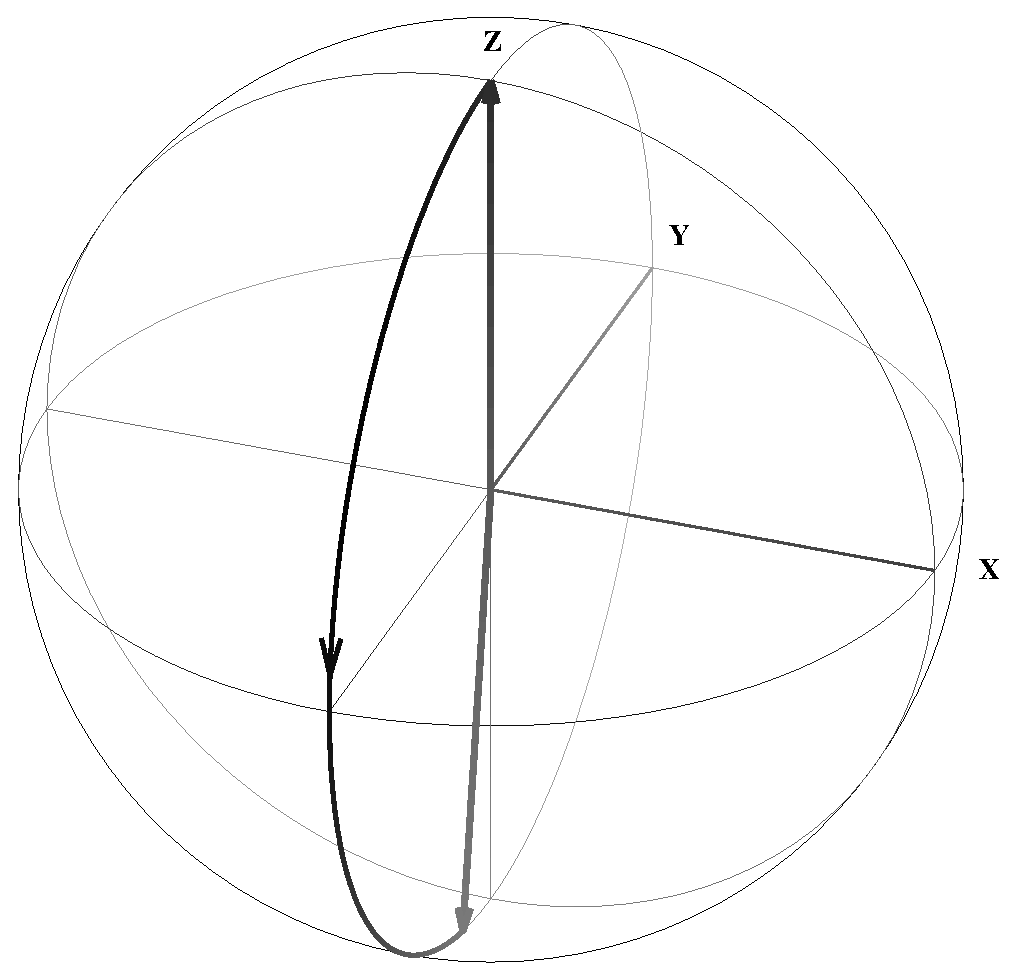
\epsfig{file=invcomp0.eps,width=2.5in}
\hspace{1em}
$b$
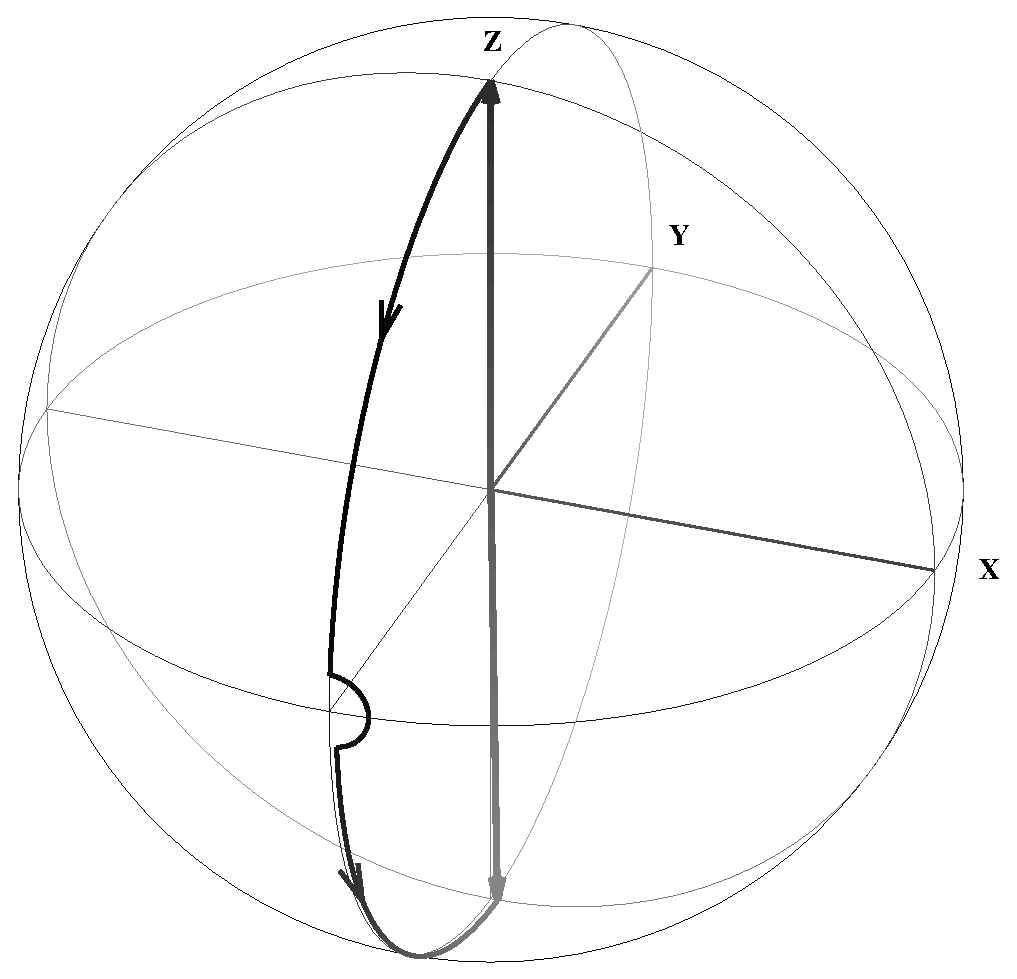
\epsfig{file=invcomp1.eps,width=2.5in}
\end{center}
\caption[Inversion composite]{Effet d'une erreur de calibration
sur l'inversion de l'aimantation d'équilibre.
A gauche l'inversion est effectuée par une impulsion $170^{\circ}_x$.
et à droite par la séquence $85^{\circ}_x$ --- $170^{\circ}_y$ --- $85^{\circ}_x$.}
\label{fig:invcomp}
\end{figure}

Une méthode rapide de mesure de $T_1$ consiste à utiliser la séquence de la figure
\ref{fig:mesuretun} et à rechercher expérimentalement la valeur $\tau_0$ de $\tau$
telle que $I(\tau_0) = 0$.
L'équation \ref{eqn:loit1} avec $\alpha = 1$ donne alors
\begin{equation}
\tau_0 = T_1 \log(2).
\end{equation}
ce qui permet d'évaluer $T_1$.

\subsection{mesure de $T_2$}
La démarche adoptée ici est la même que celle qui précède, à savoir une
"préparation" de l'aimantation qui révèle la grandeur à mesurer,
suivie de l'enregistrement du spectre proprement dit.
Pour mesurer $T_2$, il faut donc laisser évoluer l'aimantation transversale
pendant un temps $\tau$ puis détecter l'évolution libre de $\aimvec$.
Pendant le temps $\tau$, $\aimvec$ évolue sous l'action de l'offset $\omsi$
du noyau $I$ étudié, offset qui dépend de la localisation du noyau $I$
dans l'échantillon si $\bzeroz$ est inhomogène.
On mesurerait alors plutôt $T_2^*$ que $T_2$ (voir figure \ref{fig:isochrom}).
Une séquence d'écho de spin de durée $\tau$ permet de rendre l'évolution
de $\aimvec$ indépendante de $\omsi$.
Le cas où $I$ est scalairement couplé à un autre noyau de même type
sera traité en détail dans le cadre de la spectroscopie 2D $J$-résolue (---).
L'écho de spin est alors incapable de compenser l'action de l'opérateur 
de couplage qui subsiste dans l'hamiltonien réduit 
(equation \ref{eqn:hredis}) et qui introduit
une distorsion de phase.
L'analyse des données expérimentales devient alors
beaucoup plus difficile.
Toutefois, le $T_2$ d'un noyau couplé peut être mesuré
à condition que $J \tau \ll 1$ pour toutes les valeurs de $\tau$ utilisées.

En pratique, la préparation de l'aimantation consiste à faire subir
1, 2, 3, ..., $n$ séquences d'écho de spin de durées identiques $\tau_1$.
Les durées $\tau$ d'évolution de l'aimantation transversale sont alors
$\tau_1$, $2\tau_1$, $3\tau_1$, ..., $\tau_n = n\tau_1$ (Figure \ref{fig:mesuret2}).

\begin{figure}[hbt]
\begin{center}
\begin{pspicture}(0,0)(7,2)
% sequence I
\rput(0,-0.5){
\rput(1,1){
\psline(0,0)(6,0)
\rput(-0.5,0){RF($I$)}
\psline[linewidth=2mm]{-}(1,0)(1,1)
\rput(0.8,1.2){$\phi_1$}
\psline[linewidth=4mm]{-}(2.5,0)(2.5,1)
\rput(2.5,1.2){$\phi_2$}
\rput(3.9,0){
\pscurve(0,0.5)(0.5,0.25)(1.5,0)
\pscurve(0,-0.5)(0.5,-0.25)(1.5,0)
\psline(0,0.5)(0,-0.5)
}
\rput(5,0.5){$\phi_R$}
}
\rput(1,0.5){
\psline{->}(2,0)(1.1,0)
\psline{->}(3,0)(3.9,0)
\rput(2.5,0){$\tau_1$}
}
\rput(2.1,0.75){
\psline(0.25,0)(0,0)(0,1.5)(0.25,1.5)
}
\rput(4.9,0.75){
\psline(-0.25,0)(0,0)(0,1.5)(-0.25,1.5)
\rput(0.7,1.6){$n$ fois}
}
}
\end{pspicture}
\caption{\label{fig:mesuret2}
Mesure de $T_2$}
\end{center}
\end{figure}
A ce niveau de l'analyse, l'intensité du signal enregistré après
un temps d'écho $\tau_n$ est donnée par 
\begin{equation}
I(\tau_n) = \pm I(0) \exp\left(-\frac{\tau_n}{T_2}\right)
\end{equation}
Le signe de $I(\tau_n)$ dépend de la relation entre $\phi_1$ et $\phi_2$
et de la parité de $n$.
En effet, si $\phi_2 = \phi_1 \pm \pi/2$ (séquence 1), alors l'opérateur qui décrit
l'état du système juste après la première impulsion commute avec
l'opérateur associé aux impulsions de refocalisation.
Le signe de $I(\tau_n)$ est alors invariable.
Si $\phi_2 - \phi_1$ vaut 0 ou $\pi$ (séquence 2), les opérateurs en question ne commutent
pas et chaque écho multiplie $I(\tau_n)$ par $-1$.
La supériorité de la séquence 1 sur la séquence 2
est manifeste si on considère l'impact des imperfections
des impulsions de refocalisation sur le signal,
imperfections dues à une mauvaise calibration de $\buns$
(ou a son homogénéité dans l'échantillon) ainsi qu'à l'effet d'offset.
Il faut pour s'en rendre compte étudier les évènements qui se déroulent
pendant deux échos successifs (Figures \ref{fig:doublecho} et \ref{fig:cpmgcalib}).

\begin{figure}[hbt]
\begin{center}
\begin{pspicture}(0,0)(7,2)
\psline(0,0.5)(7,0.5)
\psline[linestyle=dashed,dash=2pt 2pt](0.5,0.3)(0.5,2)
\rput(0.5,0){A}
\rput(3.5,0){D}
\psline[linestyle=dashed,dash=2pt 2pt](3.5,0.3)(3.5,2)
\rput(6.5,0){G}
\psline[linestyle=dashed,dash=2pt 2pt](6.5,0.3)(6.5,2)
\rput(0.5,0.5){
\psline[linewidth=4mm]{-}(1.5,0)(1.5,1)
\psline{->}(1,1.5)(0,1.5)
\psline{->}(2,1.5)(3,1.5)
\rput(1.5,1.5){$\tau$}
\rput(1.3,-0.5){B}
\rput(1.7,-0.5){C}
}
\rput(3.5,0.5){
\psline[linewidth=4mm]{-}(1.5,0)(1.5,1)
\psline{->}(1,1.5)(0,1.5)
\psline{->}(2,1.5)(3,1.5)
\rput(1.5,1.5){$\tau$}
\rput(1.3,-0.5){E}
\rput(1.7,-0.5){F}
}
\end{pspicture}
\caption[Double écho de spin]{Double écho de spin. Les instants
marqués A à G font référence à la figure \ref{fig:cpmgcalib}.}
\label{fig:doublecho}
\end{center}
\end{figure}

Pendant les périodes de précession libre (A$\rightarrow$B, C$\rightarrow$D,
D$\rightarrow$E et F$\rightarrow$G), l'aimantation tourne d'un même angle 
autour de l'axe $OZ$ (dans cet exemple, il vaut 45\degres) et l'angle des
impulsions de refocalisation n'est pas $\pi$ (ici, il vaut 160\degres).
L'aimantation à l'instant D, dans la figure de gauche (séquence 1), 
est située au dessus du plan transversal au lieu d'être dessus,
comme ce serait le cas si l'impulsion était parfaite.
Cette erreur est compensée par le deuxième écho et l'aimantation en G
n'est que faiblement différente de celle à l'instant initial A.
La figure de droite montre que si $\phi_2 = \phi_1$ (séquence 2), l'aimantation
en D arrive en dessous du plan transversal et
s'en retrouve deux fois plus éloigné en G à l'issue du second écho.
L'effet des erreurs de calibration est alors cumulatif.

\begin{figure}[hbt]
\begin{center}
$a$
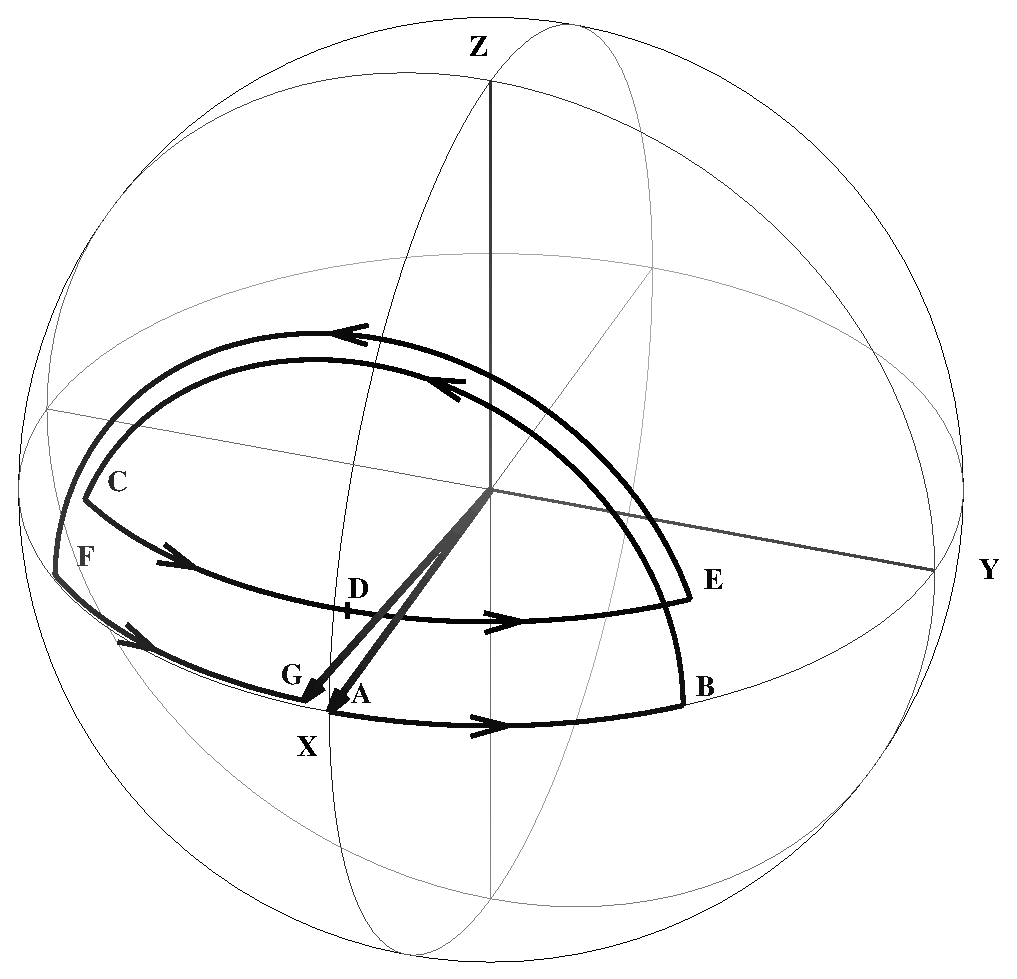
\epsfig{file=cpmgcalib0.eps,width=2.5in}
\hspace{1em}
$b$
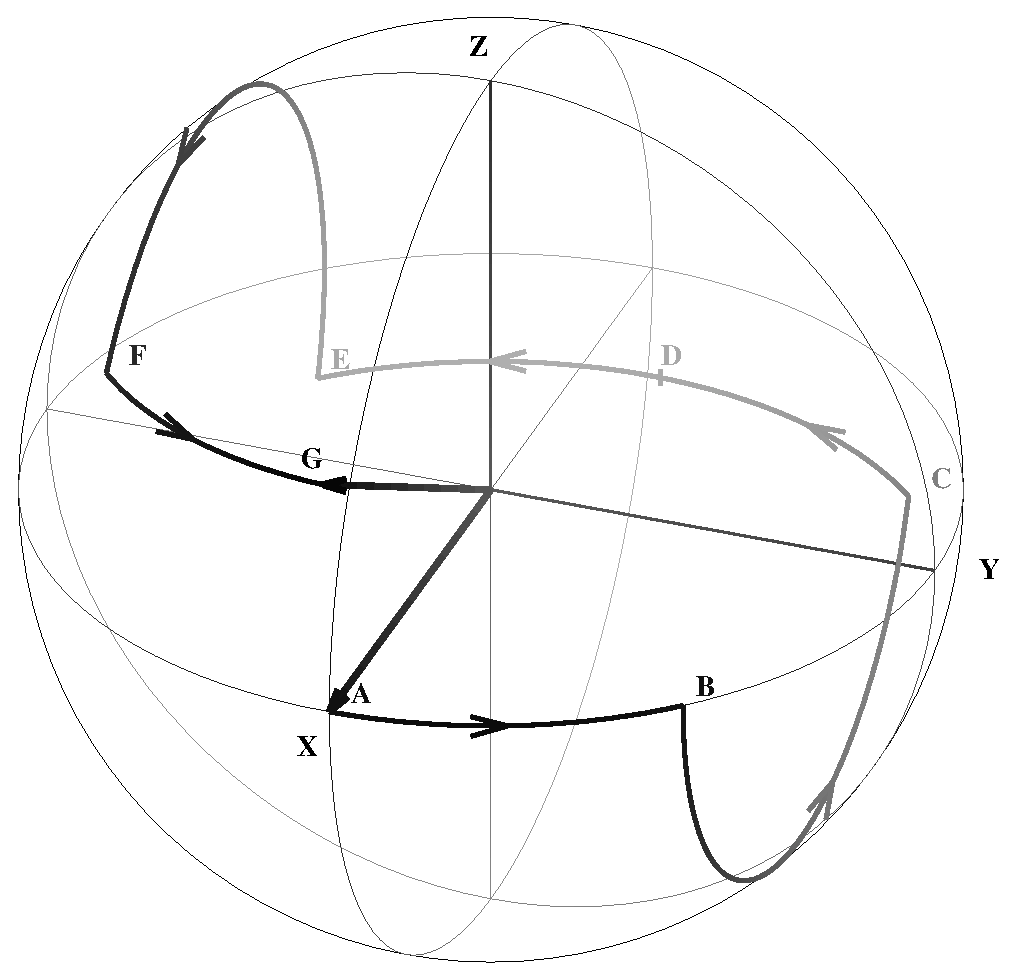
\epsfig{file=cpmgcalib1.eps,width=2.5in}
\end{center}
\caption[Séquence CPMG]{Effet d'une erreur de calibration sur l'évolution de
l'aimantation au cours d'un double écho de spin.
A gauche $\phi_2 - \phi_1 = \pi/2$ (Séquence 1, ou CPMG) 
et à droite $\phi_1 = \phi_2$ (Séquence 2, ou CP).}
\label{fig:cpmgcalib}
\end{figure}

La séquence 2 est aussi appelée séquence de Carr--Purcell.
Elle a été améliorée
par le déphasage de $\pi/2$ des impulsions de refocalisation par rapport à
l'impulsion d'excitation pour aboutir à séquence de Carr--Purcell--Meiboom--Gill
(CPMG).
L'enregistrement des signaux qu'elle produit lorsque $n$ est pair minimise
les erreurs sur la mesure de $T_2$.

La valeur de $T_2$ est obtenue à partir de la représentation graphique
de la fonction $f(\tau_n)$ définie par
\begin{equation}
f(\tau_n) = \log\left(\frac{I(\tau_n)}{I(0)}\right) = -\frac{\tau_n}{T_2}
\end{equation}
La fonction $f(\tau_n)$ est linéaire et sa pente est $-1/T_2$.

La non--équivalence d'un écho de durée totale $n\tau_1$ et de $n$ échos
de durée $\tau_1$ n'apparaît que lorsqu'on considère le mouvement
brownien des molécules au sein de l'échantillon liquide et l'existence
du gradient $\sgvec$ de $\bzerozs$, constant dans le temps, et dû au réglage imparfait
des courants dans les bobines de shim.
Il s'agit bien ici du gradient qui caractérise les inhomogénéités de $\bzerozs$ et
dont l'effet est combattu par la succession des échos de spin.

Les noyaux d'un petit élément de volume de l'échantillon
qui auraient subi un champ $\bzero(\rvec)$ au cours de la première moitié
du temps d'écho et un champ différent pendant la seconde moitié ne
verrait pas son aimantation parfaitement refocalisé à la fin de l'écho.
Un traitement plus rigoureux de cette vision simpliste des évènements
indique qu'à la fin d'un écho, le signal
recueilli est d'autant plus atténué que le gradient résiduel $\sgvec$ est intense
et que les molécules sont mobiles.
La phase du signal n'est pas affectée.
La mobilité des noyaux est caractérisée par une grandeur, le coefficient de diffusion
translationnelle, notée $D$.
Il est possible de montrer qu'à cause de la diffusion
\begin{eqnarray}
I(\tau_1) & = & I(0) \exp\left(-\frac{\tau_1}{T_2}\right)
\exp(-D\gamma^2\sgs^2\tau_1^3/12) \\
& = & I'(\tau_1) \exp(-D\gamma^2\sgs^2\tau_1^3/12)
\end{eqnarray}
où $I'$ désigne l'intensité du signal en l'absence de diffusion.
Après $n$ échos de durée $\tau_1$, l'intensité $I_n$ du signal est
\begin{equation}
I_n(\tau_n) = I'(\tau_n) \exp(-nD\gamma^2\sgs^2\tau_1^3/12)
\end{equation}
Avec un seul écho de durée $\tau_n$ l'intensité $I_1$ du signal s'écrit
\begin{eqnarray}
I_1(\tau_n) & = & I'(\tau_n) \exp(-D\gamma^2\sgs^2(n\tau_1)^3/12)\\
& = & I'(\tau_n) \exp(-nD\gamma^2(n\sgs)^2\tau_1^3/12)
\end{eqnarray}
L'utilisation de $n$ échos au lieu d'un seul
est donc équivalente à réduire d'un facteur $n$
l'intensité du gradient résiduel et donc à réduire l'effet de la diffusion
sur la mesure de $T_2$.

\chapter[RMN 2D]{Expériences à deux dimensions}

Une séquence impulsionnelle dont le but est la production d'un spectre de RMN 2D
n'est pas plus difficile à analyser qu'une séquence 1D.
Elle est en effet constituée d'impulsions de radio-fréquence et
de gradient de champ statique séparées par des délais
ou des périodes d'acquisition du signal.
L'acquis théorique des chapitres précédents trouve naturellement
ici un nouveau domaine d'application.

\section{Généralités}
\label{sec:2d:gen}
L'utilisation de la plus fréquente de la RMN 2D est
la recherche de paires de noyaux couplés.
Il est alors question de spectres 2D de corrélation des déplacements chimiques.
Cette expression indique que le déplacement chimique d'un noyau
est corrélé à celui d'un d'autre noyau si ces deux noyaux sont couplés ensemble.
L'acronyme COSY a été formée à partir de l'expression "COrrelation SpectroscopY".
L'expérience historique relatée en 1971 a été suivie de très nombreux
développements et d'autres séquences impulsionnelles dédiées à la spectroscopie de 
corrélation ont vu le jour et reçu diverses appellations.

Le grand intérêt de la RMN 2D est de concentrer sur un seul spectre l'information
relative à toutes les paires de noyaux, pour un type de couplage donné.
On distingue en effet les spectres 2D homonucléaires (\prot -- \prot, comme les spectres COSY et NOESY)
des spectres 2D hétéronucléaires (\prot -- \carb par exemple, comme le spectre HSQC).
La recherche de paires de noyaux couplés est une étape essentielle à
l'interprétation des spectres de molécules complexes.
En effet, l'existence
d'un couplage scalaire indique que les noyaux concernés sont séparés par un
petit nombre de liaisons chimiques ; elle fournit donc une information
sur la connectivité des atomes d'une molécule, c'est-à-dire sur sa formule
développée plane.
De plus, un couplage dipolaire est une source de relaxation croisée
et révèle donc une proximité spatiale entre les noyaux.
Un spectre NOESY permet ainsi de préciser la configuration d'une molécule,
c'est-à-dire sa structure tridimensionnelle.

En plus de la corrélation des déplacements chimiques,
une autre famille d'expériences de RMN 2D produit des spectres
dits "de séparation des interactions".
Dans cette catégorie, un spectre $J$-résolu fournit une vision
séparée des déplacements chimiques
et des motifs de couplage scalaire. 
Cette expérience facilite la mesure
de ces constantes et vient compléter les informations conformationnelles apportées
par l'expérience NOESY, elle permet
de plus une lecture simplifiée des déplacements chimiques

Pour tenter de réduire la difficulté d'apprentissage 
des concepts spécifiques à la RMN 2D (ou nD...) la séquence COSY
"à un seul noyau" sera d'abord traitée.
Il n'y a aucun intérêt à utiliser la séquence COSY sur des systèmes à un spin
puisque le but de la séquence COSY
est de révéler les couplages entre deux noyaux.
Toutefois, l'analyse de la séquence COSY sur un tel système
est commode pour introduire le concept de modulation et montrer
comment le problème central de la détermination du signe des fréquences dans
les deux dimensions a été résolu.
Les résultats généraux obtenus à partir de cet exemple
faciliteront l'étude des autres séquences.
La COSY "à un noyau" ne faisant pas intervenir de système de spins couplés,
la description vectorielle de l'évolution de l'aimantation nucléaire est suffisante.
Cela réduit au minimum l'aspect calculatoire, souvent dissuasif, des explications
relatives à la compréhension de la RMN 2D.

\section{La COSY "à un noyau"}
\label{sec:2d:cosy1noyau}
\subsection{Séquence}
\label{sec:2d:cosy1noyau:seq}
La séquence de base, figure \ref{fig:cosydebase}, est constituée d'un délai de relaxation,
d'une impulsion d'excitation, d'un délai d'évolution de durée nommé $t_1$, 
d'une impulsion dite "de transfert" et d'une période
d'acquisition où le signal est mesuré aux instants $t_2$.
Cette séquence n'est autre qu'une séquence 1D un peu particulière.
L'expérience n'acquiert l'appellation 2D que si elle est réalisée pour plusieurs valeurs
de $t_1$.
Les angles de nutation des deux impulsions seront considérés comme égaux à $\pi/2$.
Le signal enregistré est une fonction de $t_2$  mais aussi du temps 
$t_1$ et des phase $\phi_1$ et $\phi_2$ des impulsions.
En fait, seule la phase relative des impulsions est significative puisque leur augmentation
simultanée de $\pi/2$ produit une multiplication du signal par $i$
qui peut être compensée en augmentant la phase du récepteur de $\pi/2$.
Le système étudié est un ensemble de noyaux identiques notés
$I$ et caractérisés par leur offset $\omsi$
et leurs temps de relaxation $T_{1I}$ et $T_{2I}$.
L'effet des inhomogénéités de $\bzeros$ ne sera pas pris en compte dans un premier temps.

\begin{figure}[hbt]
\begin{center}
\begin{pspicture}(0,0)(7,3)
% sequence I
\rput(1,1.5){
\psline(0,0)(6,0)
\rput(-0.5,0){RF($I$)}
\psline[linewidth=2mm]{-}(1,0)(1,1)
\rput(1,1.2){$\phi_1$}
\psline[linewidth=2mm]{-}(4,0)(4,1)
\rput(4,1.2){$\phi_2$}
\rput(4.1,0){
\pscurve(0,0.5)(0.5,0.25)(1.5,0)
\pscurve(0,-0.5)(0.5,-0.25)(1.5,0)
\psline(0,0.5)(0,-0.5)
}
\rput(5,0.5){$\phi_R$}
}
% time marks
\rput(1,0.5){
\psline{->}(0,0)(6,0)
\rput(6.2,0){$t$}
\psline[linewidth=0.25mm,linestyle=dashed]{-}(0.9,0.8)(0.9,-0.2)
\rput(0.8,-0.4){A}
\psline[linewidth=0.25mm,linestyle=dashed]{-}(1.1,0.8)(1.1,-0.2)
\rput(1.2,-0.4){B}
\rput(2.5,0.5){$t_1$}
\psline[linewidth=0.25mm,linestyle=dashed]{-}(3.9,0.8)(3.9,-0.2)
\rput(3.8,-0.4){C}
\psline[linewidth=0.25mm,linestyle=dashed]{-}(4.1,0.8)(4.1,-0.2)
\rput(4.2,-0.4){D}
\psline[linewidth=0.25mm,linestyle=dashed]{-}(5,0.8)(5,-0.2)
\rput(5.3,0.5){$t_2$}
}
\end{pspicture}
\caption{\label{fig:cosydebase}
Séquence COSY}
\end{center}
\end{figure}

\subsection{Modulation d'amplitude, méthode de States}
\label{sec:2d:cosy1noyau:amp}
L'aimantation initiale
\begin{equation}
\aimvec(t_A) = \aimzeros\coo{0}{0}{1}
\end{equation}
devient
\begin{equation}
\aimvec(t_B) = \aimzeros\coo{0}{-1}{0} \qsiq \phi_1 = 0 \qetq
\aimvec(t_B) = \aimzeros\coo{1}{0}{0} \qsiq \phi_1 = \pi/2
\end{equation}
après la première impulsion.
Après le délai de durée $t_1$, l'aimantation devient
\begin{eqnarray}
\label{eqn:rmn2d1:tcs}
\aimvec(t_C) & = & \aimzeros\coo{\sin(\omsi t_1)}{-\cos(\omsi t_1)}{0} \qsiq \phi_1 = 0 \\
\label{eqn:rmn2d1:tcc}
\aimvec(t_C) & = & \aimzeros\coo{\cos(\omsi t_1)}{\sin(\omsi t_1)}{0} \qsiq \phi_1 = \pi/2
\end{eqnarray}
en considérant que ni la relaxation transversale ni la relaxation longitudinale
ne sont intervenus pendant $t_1$.
En réalité, leur action se traduit par le facteur d'amortissement de l'aimantation transversale
$r_{2I}(t_1) = \exp(-t_1/T_{2I})$ et le facteur de "repousse" de l'aimantation longitudinale
$r_{1I}(t_1) = 1 - \exp(-t_1/T_{1I})$ (équations \ref{eqn:relaxlong} et \ref{eqn:relaxtrans}),
si bien que les équations \ref{eqn:rmn2d1:tcs} et \ref{eqn:rmn2d1:tcc} deviennent :
\begin{eqnarray}
\aimvec(t_C) & = & 
\aimzeros\coo{\sin(\omsi t_1) r_{2I}(t_1)}{-\cos(\omsi t_1) r_{2I}(t_1)}{r_{1I}(t_1)}
\qsiq \phi_1 = 0 \\
\aimvec(t_C) & = & 
\aimzeros\coo{\cos(\omsi t_1) r_{2I}(t_1)}{\sin(\omsi t_1) r_{2I}(t_1)}{r_{1I}(t_1)} 
\qsiq \phi_1 = \pi/2
\end{eqnarray}
La seconde impulsion, de phase 0 ou $\pi$, préserve la composante sur l'axe $OX$ de
l'aimantation transversale et transfère l'autre sur l'axe $OZ$. 
La composante initialement présente sur $OZ$ est basculée dans le plan 
transversal sur l'axe $OY$.
Avec $\phi_2$ = 0,
\begin{eqnarray}
\label{eqn:rmn2d1aimxx}
\aimvec(t_D) & = &
\aimzeros\coo{\sin(\omsi t_1) r_{2I}(t_1)}{-r_{1I}(t_1)}{-\cos(\omsi t_1) r_{2I}(t_1)}
\qsiq \phi_1 = 0 \\
\label{eqn:rmn2d1aimyx}
\aimvec(t_D) & = & 
\aimzeros\coo{\cos(\omsi t_1) r_{2I}(t_1)}{-r_{1I}(t_1)}{\sin(\omsi t_1) r_{2I}(t_1)}
\qsiq \phi_1 = \pi/2
\end{eqnarray}
Dans les deux cas, la composante de l'aimantation sur l'axe $OX$ immédiatement avant le début
de l'acquisition du signal est identique à celle obtenue par application
d'une unique impulsion de phase $y$, à ceci près que l'\emph{amplitude}
est en ici modulée par un facteur qui dépend du produit $\omsi t_1$.
La modulation est dite "en sinus" quand les axes de rotation associés aux deux impulsions
sont colinéaires et "en cosinus" quand ils sont orthogonaux.

L'aimantation présente sur l'axe $OX$ donne lieu aux signaux
\begin{eqnarray}
s_S(t_1, t_2) & = & s_0 \sin(\omsi t_1) r_{2I}(t_1) \times \exp(i \omsi t_2 ) r_{2I}(t_2) \\
s_C(t_1, t_2) & = & s_0 \cos(\omsi t_1) r_{2I}(t_1) \times \exp(i \omsi t_2 ) r_{2I}(t_2)
\end{eqnarray}
où les indices $S$ et $C$ font référence aux deux types de modulation d'amplitude et $s_0$
est l'intensité du {\FID} obtenu par une seule impulsion de phase $\pi/2$.
La quantité $s_0$ est un nombre réel, ce qui sous-entend que le détecteur n'introduit pas
de déphasage du signal. Le facteur multiplicatif $s_0$ sera considéré par la suite 
comme égal à 1, sans perte de généralité pour l'exposé.
La partie réelle des signaux temporels est représentée sur la partie gauche
de la figure \ref{fig:modulampl}.
La TF de ces signaux, considérés comme des fonctions de la variable 
temporelle d'acquisition $t_2$ donne
\begin{eqnarray}
f_S(t_1, \Omega_2) & = & \sin(\omsi t_1) r_{2I}(t_1)
\times (A_I(\Omega_2-\omsi) + iD_I(\Omega_2-\omsi)) \\
f_C(t_1, \Omega_2) & = & \cos(\omsi t_1) r_{2I}(t_1)
\times (A_I(\Omega_2-\omsi) + iD_I(\Omega_2-\omsi))
\end{eqnarray}
où $A_I(\Omega_2)$ et $D_I(\Omega_2)$ sont les fonctions lorentziennes en absorption
et en dispersion centrées autour de la fréquence nulle.
La temps d'acquisition étant nommé $t_2$, la variable fréquentielle
associée a été nommée $\Omega_2$.
\begin{figure}[hbt]
\begin{center}
\begin{pspicture}(-0.5,-1)(13.5,7)
\psset{unit=5mm,labelsep=3pt}
\rput(0,0){
\rput(0,0){
\multido{\i=0+1}{24}
{
  \FPeval{yy}{\i/24*5}
  \FPeval{absc}{\i*0.1}
  \FPeval{ordo}{\i*0.5}
  \FPupn{facta}{yy 0.3 mul 2 mul \FPpi{} mul sin}
  \FPupn{factb}{yy 4 div neg exp}
  \FPupn{factc}{0.8}
  \FPupn{fact}{facta factb mul factc mul}
  \rput(\absc,\ordo)
  {
    \psplot[algebraic,plotpoints=200]{0}{5}{\fact*cos(x*2*\FPpi)*(\FPe^(-x/4))}
  }
}
\rput(-1,0){\psline{->}(0,0)(2.4,12)\uput[70](2.4,12){$t_1$}}
\rput(0,-1){\psline{->}(0,0)(5,0)\uput[-70](5,0){$t_2$}}
\rput(2.5,-2){$s_S(t_1,t_2)$}
}
\rput(6,0){
\multido{\i=0+1}{24}
{
  \FPeval{yy}{\i/24*5}
  \FPeval{absc}{\i*0.1}
  \FPeval{ordo}{\i*0.5}
  \FPupn{facta}{yy 0.3 mul 2 mul \FPpi{} mul cos}
  \FPupn{factb}{yy 4 div neg exp}
  \FPupn{factc}{0.8}
  \FPupn{fact}{facta factb mul factc mul}
  \rput(\absc,\ordo)
  {
    \psplot[algebraic,plotpoints=200]{0}{5}{\fact*cos(x*2*\FPpi)*(\FPe^(-x/4))}
  }
}
\rput(0,-1){\psline{->}(0,0)(5,0)\uput[-70](5,0){$t_2$}}
\rput(2.5,-2){$s_C(t_1,t_2)$}
}
}
%
\rput(14,0){
\rput(0,0){
\multido{\i=0+1}{24}
{
  \FPeval{yy}{\i/24*5}
  \FPeval{absc}{\i*0.1}
  \FPeval{ordo}{\i*0.5}
  \FPupn{facta}{yy 0.3 mul 2 mul \FPpi{} mul sin}
  \FPupn{factb}{yy 4 div neg exp}
  \FPupn{factc}{0.9}
  \FPupn{fact}{facta factb mul factc mul}
  \rput(\absc,\ordo)
  {
    \psplot[algebraic,plotpoints=200]{0}{5}{\fact/(1+((x-2.5)/0.2)^2)}
  }
}
\rput(-1,0){\psline{->}(0,0)(2.4,12)\uput[70](2.4,12){$t_1$}}
\rput(0,-1){\psline{<-}(0,0)(5,0)\uput[-110](0,0){$\Omega_2$}}
\rput(2.5,-2){$f_S(t_1,\Omega_2)$}
}
\rput(6,0){
\multido{\i=0+1}{24}
{
  \FPeval{yy}{\i/24*5}
  \FPeval{absc}{\i*0.1}
  \FPeval{ordo}{\i*0.5}
  \FPupn{facta}{yy 0.3 mul 2 mul \FPpi{} mul cos}
  \FPupn{factb}{yy 4 div neg exp}
  \FPupn{factc}{0.9}
  \FPupn{fact}{facta factb mul factc mul}
  \rput(\absc,\ordo)
  {
    \psplot[algebraic,plotpoints=200]{0}{5}{\fact/(1+((x-2.5)/0.2)^2)}
  }
}
\rput(0,-1){\psline{<-}(0,0)(5,0)\uput[-110](0,0){$\Omega_2$}}
\rput(2.5,-2){$f_C(t_1,\Omega_2)$}
}
}
\end{pspicture}
\caption{\label{fig:modulampl}
Signaux temporels 2D modulés en amplitude (à gauche) et leur TF (à droite)}
\end{center}
\end{figure}
La partie réelle des spectres, dont les intensités sont
modulées en sinus et en cosinus (voir la partie droite de la figure \ref{fig:modulampl})
peuvent être combinées pour donner un signal complexe virtuel (c'est-à-dire fabriqué
sans avoir été enregistré physiquement) $f(t_1, \Omega_2)$
dont l'intérêt apparaîtra bientôt.
\begin{eqnarray}
f(t_1, \Omega_2) & = & \reel(f_S(t_1, \Omega_2)) + i\reel(f_C(t_1, \Omega_2)) \\
\label{eq:rmn2d1:virtuel}
                 & = & i \exp(-i \omsi t_1) r_{2I}(t_1) \times A_I(\Omega_2-\omsi)
\end{eqnarray}
Ainsi $f(t_1, \Omega_2)$, considéré pour chaque valeur de $\Omega_2$,
varie en fonction de $t_1$ comme un {\FID} ordinaire.
Avec la méthode choisie pour la construction de la fonction $f$,
c'est la pulsation $-\omsi$ qui intervient pendant $t_1$
puisque $\sin x + i\cos x = i(\cos x - i \sin x) = i\exp(-ix)$.
De la même manière qu'un {\FID} est enregistré à partir de $t_2 = 0$ par intervalles
$\delta t_2 = 1/\Delta F_2$ pour
disposer d'une fenêtre spectrale de largeur $\Delta F_2$,
il suffit de faire varier $t_1$ à partir de 0 
par pas $\delta t_1 = 1/\Delta F_1$ pour déterminer
la fréquence d'évolution de l'aimantation pendant $t_1$
à l'intérieur d'une fenêtre spectrale de largeur $\Delta F_1$.
La TF de toutes les fonctions $S(t_1, \Omega_2)$, chacune correspondant 
à une valeur particulière de $\Omega_2$ et étant donc considérée comme une fonction
de la variable temporelle $t_1$, fournit
\begin{equation}
S(\Omega_1, \Omega_2) = i \times (A_I(\Omega_1+\omsi) + iD_I(\Omega_1+\omsi)) 
\times A_I(\Omega_2-\omsi)
\end{equation}
Une correction de phase de $\pi/2$ (une multiplication par $-i$) et la conservation de la seule
partie réelle conduit à
\begin{equation}
S(\Omega_1, \Omega_2) = A_I(\Omega_1+\omsi)  \times A_I(\Omega_2-\omsi)
\end{equation}
qui correspond à une raie élémentaire en absorption pure d'un spectre de RMN 2D,
et dont le maximum se trouve à $(\Omega_1, \Omega_2) = (-\omsi, \omsi)$.
Dans la pratique,le spectre 2D
est représenté en fonction de $-\Omega_1$ (sur un axe vertical dirigé de haut en bas)
et de $\Omega_2$ (sur un axe horizontal dirigé, comme en RMN 1D, de droite à gauche)
de sorte que l'évolution de l'aimantation
d'un même noyau pendant $t_1$ et $t_2$ se traduit par un pic situé sur la diagonale principale
du spectre, orientée du haut à droite vers le bas à gauche
dans le sens des déplacements chimiques croissants.
Les axes verticaux et horizontaux sont respectivement désignés sous le noms d'axes $F_1$ et $F_2$.
La figure \ref{fig:raies2D} fournit une représentation graphique
des formes de raies usuelles en RMN 2D.

\renewcommand{\baselinestretch}{1}
\normalsize
\begin{figure}[hbt]
\begin{center}

\begin{tabular}{llll}
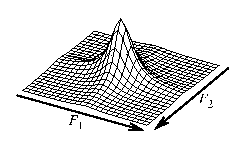
\includegraphics[scale=0.9]{ContSurf/surf1.eps} & 
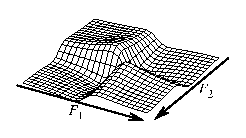
\includegraphics[scale=0.9]{ContSurf/surf2.eps} & 
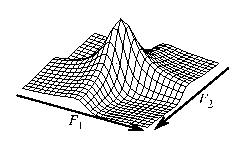
\includegraphics[scale=0.9]{ContSurf/surf3.eps} & 
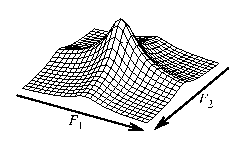
\includegraphics[scale=0.9]{ContSurf/surf4.eps} \\
\rule[0mm]{0mm}{2mm} \\
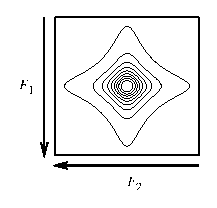
\includegraphics[scale=0.9]{ContSurf/cont1.eps} & 
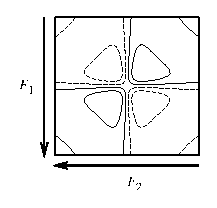
\includegraphics[scale=0.9]{ContSurf/cont2.eps} & 
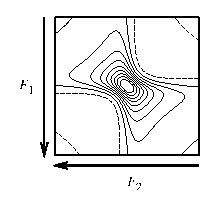
\includegraphics[scale=0.9]{ContSurf/cont3.eps} & 
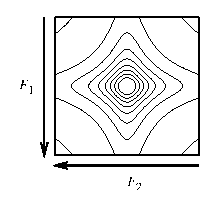
\includegraphics[scale=0.9]{ContSurf/cont4.eps} \\
\myc{\raisebox{-0.5ex}[0pt]{Double}} &
\myc{\raisebox{-0.5ex}[0pt]{Double}} &
\myc{\raisebox{-0.5ex}[0pt]{Phase}} \\
\myc{Absorption} & 
\myc{Dispersion} & 
\myc{Twist} & 
\myc{\raisebox{1.25ex}[0pt]{Magnitude}}

\end{tabular}
\caption{\label{fig:raies2D}Formes de raies en RMN 2D}
\end{center}
\end{figure}
\renewcommand{\baselinestretch}{1.5}
\normalsize
Le cas particulier qui a été détaillé dans les paragraphes précédents est celui où 
le noyau dont l'aimantation évolue pendant $t_1$ ($I$) est le même que celui
dont l'aimantation évolue pendant $t_2$.
Dans le cas général, il faut considérer que l'aimantation d'un noyau $S$,
qui évolue pendant $t_1$, est transférée sur un noyau $I$ avant la détection
du signal créé par ce dernier.
Alors, les signaux enregistrés dépendent de $t_1$ au travers de facteurs
$\sin(\omss t_1)$ ou $\cos(\omss t_1)$ multipliés par un facteur d'amortissement
$r_{2S}=\exp(-t_1/T_{2S})$ où $\omss$ et $T_{2S}$ caractérisent le noyau S :
\begin{eqnarray}
s_S(t_1, t_2) & = & \sin(\omss t_1) r_{2S}(t_1) \times \exp(i \omsi t_2 ) r_{2I}(t_2) \\
s_C(t_1, t_2) & = & \cos(\omss t_1) r_{2S}(t_1) \times \exp(i \omsi t_2 ) r_{2I}(t_2)
\end{eqnarray}
L'expérience COSY, effectuée sur un système à un spin, ne peut pas donner
lieu à un transfert d'aimantation, ce qui conduit à identifier $S$ avec $I$.
D'une manière encore plus générale, la fréquence d'évolution pendant $t_1$
peut n'être ni $\omsi$ ni $\omss$, mais une autre comme $\omsi + \omss$, fréquence
d'évolution des états à double quanta dans un spectre INADEQUATE
ou encore $\pi J$ dans un spectre $J$-résolu.

Ce qui vient d'être décrit passe sous silence les signaux issus des composantes de
l'aimantation sur l'axe $OY$ décrites dans les équations
\ref{eqn:rmn2d1aimxx} et \ref{eqn:rmn2d1aimyx}.
Leur évolution en fonction de $t_1$ ne comporte aucune partie oscillante et sa TF selon $t_1$
produit un pic centré autour de la fréquence $\Omega_1$ nulle.
En effet, dans le facteur $1-\exp(-t_1/T_{1I})$, le terme 1 conduit à un
spectre nul partout sauf
pour $\Omega_1 = 0$ et le terme $-\exp(-t_1/T_{1I})$ conduit à une raie lorentzienne
centrée sur $\Omega_1 = 0$.
Si $t_1$ est suffisamment grand par rapport à $T_{1I}$ pour que $r_{1I}$ soit
significativement non nul, alors des pics indésirables sont visibles sur l'axe 
$F_1$ du spectre.
Ces pics axiaux sont éliminés par action du programme de phase de la séquence.
Si $\phi_2 = \pi$ au lieu de $0$, alors, à l'instant $t=t_D$
la composante de l'aimantation sur l'axe $OX$ est inchangée et celle sur $OY$
est inversée. 
Le signal indésirable est donc éliminé par addition des {\FID} produits
avec $\phi_2 = 0$ et $\phi_2 = \pi$.
Le nombre de scans minimum par valeur de $t_1$ nécessaire pour obtenir un spectre 2D
dépourvu de pic axiaux est donc de 4, 2 pour chaque type de modulation.

L'ensemble de la procédure d'acquisition et de traitement qui vient d'être décrite
fournit à la fois des pics en absorption pure et permet de déterminer le signe
de la fréquence d'évolution de l'aimantation pendant $t_1$.
Ces deux objectifs sont atteints parce qu'il est possible d'enregistrer séparément
les signaux modulés en sinus et en cosinus.
En imaginant que seule la modulation en cosinus ait été enregistrée,
il serait impossible de distinguer $\cos(\omsi t_1)$ de $\cos(-\omsi t_1)$
et avec la modulation en sinus de distinguer $\sin(\omsi t_1)$ de -$\sin(-\omsi t_1)$.
La procédure est désignée parfois par l'acronyme SHR,
formé à partir des intiales des auteurs de la publication
qui l'a formalisée : States, Haberkorn et Ruben.
Il est plus commun de parler de la méthode "States", caractérisée
par l'enregistrement d'un signal modulé en sinus
et d'un signal modulés en cosinus, les deux étant enregistrés
pour chaque valeur de $t_1$ multiple entier de la période
d'échantillonnage $\delta t_1 = 1/\Delta F_1$, et comme
indiqué sur la figure \ref{fig:amplvariant}.
\begin{figure}[hbt]
\begin{center}
\begin{pspicture}(0,1)(14,3.5)
\psset{unit=8mm}
\rput(1,2){%
  \psline{->}(-0.5,0)(4.5,0)\uput[-90](4.5,0){$\tau$}
  \multido{\i=0+1}{5}{%
    \psline(\i,0.1)(\i,-0.1)\uput[270](\i,-0.1){\i}
  }
  \multido{\r=0.5+0.5}{4}{%
    \psline[linestyle=dotted](-0.5,\r)(4.5,\r)
  }
  \uput[180](-0.5,0.5){sin}
  \uput[180](-0.5,1.0){cos}
  \uput[180](-0.5,1.5){-sin}
  \uput[180](-0.5,2.0){-cos}
  \rput(2,-1.5){States}
  \multido{\i=0+1}{5}{%
    \psdots[dotstyle=diamond*,dotscale=1.5](\i,0.5)
    \psdots[dotstyle=diamond*,dotscale=1.5](\i,1.0)
  }
}

\rput(6.5,2){%
  \psline{->}(-0.5,0)(4.5,0)\uput[-90](4.5,0){$\tau$}
  \multido{\i=0+1}{5}{%
    \psline(\i,0.1)(\i,-0.1)\uput[270](\i,-0.1){\i}
  }
  \multido{\r=0.5+0.5}{4}{%
    \psline[linestyle=dotted](-0.5,\r)(4.5,\r)
  }
  \rput(2,-1.5){States-TPPI}
  \multido{\i=0+2}{3}{%
    \psdots[dotstyle=diamond*,dotscale=1.5](\i,0.5)
    \psdots[dotstyle=diamond*,dotscale=1.5](\i,1.0)
  }
  \multido{\i=1+2}{2}{%
    \psdots[dotstyle=diamond*,dotscale=1.5](\i,1.5)
    \psdots[dotstyle=diamond*,dotscale=1.5](\i,2.0)
  }
}

\rput(12,2){%
  \psline{->}(-0.5,0)(4.5,0)\uput[0](4.5,0){%
    $\tau = \displaystyle\frac{t_1}{\delta t_1}$}
  \multido{\i=0+1}{5}{%
    \psline(\i,0.1)(\i,-0.1)\uput[270](\i,-0.1){\i}
  }
  \multido{\r=0.5+0.5}{4}{%
    \psline[linestyle=dotted](-0.5,\r)(4.5,\r)
  }
  \rput(2,-1.5){TPPI}
  \multido{\i=0+2}{2}{%
    \rput(\i,0){%
      \multido{\rx=0.0+0.5,\ry=0.5+0.5}{4}{
        \psdots[dotstyle=diamond*,dotscale=1.5](\rx,\ry)
      }
    }
  }
  \rput(4,0){
    \multido{\rx=0.0+0.5,\ry=0.5+0.5}{2}{
      \psdots[dotstyle=diamond*,dotscale=1.5](\rx,\ry)
    }
  }
}
\end{pspicture}
\end{center}
\caption{\label{fig:amplvariant} Les modes d'acquisition en modulation d'amplitude}
\end{figure}

\subsection{Méthode States-TPPI}
\label{sec:2d:cosy1noyau:st}
Une variante de la méthode States permet de déplacer les pics axiaux de leur position
centrale vers les bords de la fenêtre spectrale en $F_1$, c'est-à-dire
à un endroit où ils sont potentiellement moins gênants.
L'échantillonnage du signal est ici encore effectuée
par incrémentation de $t_1$ à partir d'une valeur nulle et par pas $\delta t_1 = 1/\Delta F_1$.
Les signaux $s_S(t_1 = 0, t_2)$ et $s_C(t_1 = 0, t_2)$
sont enregistrés comme précédemment,
$\phi_2$ et $\phi_R$ restant nuls pendant toute l'acquisition des données.
Les signaux à $t_1 = \delta t_1$ sont enregistrés avec $\phi_1 = \pi$.
Chaque incrémentation ultérieure de $t_1$ est aussi accompagnée d'une incrémentation de $\pi$
de la valeur de $\phi_1$, comme indiqué au milieu de la figure \ref{fig:amplvariant}.
Cette incrémentation de phase proportionnelle au temps (sous-entendu $t_1$)
ou "Time Proportional Phase Increment", TPPI, donne à la méthode le nom "States--TPPI".
Elle cause une inversion de l'aimantation sur l'axe $OX$ en $t=t_B$
et donc une multiplication des signaux $s_S$ et $s_C$
par -1 une fois sur deux, lorsque $\tau = t_1/\delta t_1$ est impair.
Le signal complexe "virtuel" $f'(t_1, \Omega_2)$ construit après TF des signaux selon $t_2$
se déduit de celui obtenu par la méthode States selon
\begin{equation}
f'(t_1, \Omega_2) = f(t_1, \Omega_2) \exp(i \pi \tau)
\end{equation}
où $\tau$ est le nombre d'incréments de $t_1$ effectués.
Le signal indésirable produit pendant $t_2$
par la relaxation longitudinale pendant $t_1$
ne dépend pas de $\phi_1$ puisque la repousse de l'aimantation longitudinale
commence toujours à partir de zéro après la première impulsion.
Le facteur $\exp(i \pi \tau)$ vaut alternativement 1 et -1 à chaque modification de $t_1$.
Ainsi
\begin{eqnarray}
\exp(i \pi \tau) & = & \exp(2 i \pi \tau \delta t_1 \Delta F_1 / 2) \\
              & = & \exp(i(2\pi\Delta F_1 / 2) t_1)
\end{eqnarray}
et donc d'après l'équation \ref{eq:rmn2d1:virtuel}
\begin{equation}
f'(t_1, \Omega_2) = i \exp(-(\omsi-(2\pi\Delta F_1 / 2)) t_1) r_{2I}(t_1) \times A_I(\Omega_2-\omsi)
\end{equation}
La fréquence en $F_1$ du pic souhaité est donc décalée de $-\Delta F_1/2$ et celle
du pic indésirable est restée à l'identique, c'est-à-dire à 0.
La permutation des deux parties de spectre qui correspondent aux intervalles
de fréquence $[0, \Delta F_1/2[$ et $[-\Delta F_1/2, 0[$ restaure l'apparence usuelle
du spectre tout en plaçant le pic précédemment axial vers le bord de la fenêtre spectrale,
comme souhaité. 
De plus, rien n'interdit d'utiliser la procédure States--TPPI avec deux scans pour
chaque valeur de $t_1$ et chaque type de modulation, avec alternance de $\phi_2$
à $\phi_R$ constant, afin d'éliminer le pic non désiré.
Cela double le temps d'acquisition minimal de l'enregistrement mais se justifie
si l'amélioration du rapport signal sur bruit est nécessaire.

\subsection{Méthode TPPI}
\label{sec:2d:cosy1noyau:tppi}
Une troisième possibilité existe pour créer un pic en absorption pure à partir des signaux
modulés en amplitude.
Elle est calquée sur le "Redfield trick" décrit au paragraphe \ref{sec:redfield}, sauf 
que l'alternance dans la sélection du canal de détection est remplacée par 
l'alternance des modulations en sinus et cosinus.
L'incrément de $t_1$ est alors la moitié de celui requis par la méthode States.
L'augmentation de $t_1$ s'accompagne d'une augmentation de la phase de $\phi_1$ d'une valeur
de $\pi/2$ ce qui confère le nom de TPPI à la méthode, à ne pas confondre avec States--TPPI !
Les {\FID} sont alors modulés successivement en sinus, cosinus, $-$sinus, $-$cosinus, sinus, etc...,
comme indiqué par la figure \ref{fig:amplvariant}.
Le doublement de la largeur de la fenêtre spectrale en $F_1$ consécutive à la division
par 2 de $\delta t_1$ est nécessaire puisque les fréquences d'évolution apparaissent
comme augmentées de $\Delta F_1 / 2$.
La TF des colonnes du tableau des données nécessite l'emploi de l'algorithme de TF
adapté aux données réelles et dans lequel les spectres ne sont calculés
que pour les fréquences positives.
La fréquence nulle se trouvant au bord de la fenêtre spectrale (au lieu d'être
au milieu lorsque l'algorithm de FT des données complexes est utilisé),
les pics issus de la relaxation longitudinale pendant $t_1$ n'occupent pas
le centre du spectre.

\subsection{Modulation de phase}
\label{sec:2d:cosy1noyau:phase}
Une étape de phasage des spectres 2D est nécessaire pour présenter
les pics en double absorption car $s_0$ n'est un nombre réel que dans
le cadre d'une étude théorique. 
Les spectres produits par les méthodes States ou TPPI ou leurs variantes
sont pour cela communément appelés "spectres phasés".
Le phasage nécessite un logiciel dédié et un ordinateur
tout-à-fait banal selon les critères actuels, mais il n'en a pas toujours été ainsi.

Une procédure d'acquisition et de traitement des données, encore utilisée aujourd'hui,
résout le problème du signe des fréquences pendant $t_1$ mais fournit des signaux
qu'il faut apodiser de manière particulière et présenter en magnitude pour être regardables,
mais évitent, comme il sera vu ci-après, l'opération de phasage.
L'idée est ici de produire une \emph{modulation de phase} à partir de signaux
modulés en amplitude. 
Comme cela sera expliqué par la suite, certaines séquences ne sont capable de produire
qu'un seul de type de modulation de phase (l'expérience $J$-résolue)
et d'autres de produire deux types de modulation
de phase (N et P, ou écho et anti--écho) qui, une fois les signaux combinés ensemble,
fournissent des signaux modulés en sinus et cosinus et susceptibles d'être traités comme
exposé ci-dessus.

Produire pendant $t_1$ une modulation de phase de type N, aussi appelée "écho",
(voir ci-après pour l'origine de ces dénominations) revient, dans
le cas général à fabriquer un signal
$s_N(t_1, t_2)$ proportionnel à $\exp(-i \omss t_1)$ et à $\exp(i \omsi t_2)$.
L'indice N se rapporte au fait que la fréquence $\omss$ intervient par
sa forme $\emph{n}$égative.
La présence du facteur $\exp(-i \omss t_1)$ assure que le signe de la
fréquence d'évolution de l'aimantation pendant $t_1$ est déterminé
sans ambiguïté.
Le signal $s_N$ s'obtient aisément à partir des signaux $s_S$ et et $s_C$
\begin{eqnarray}
s_N(t_1, t_2) & = & s_S(t_1, t_2) + i s_C(t_1, t_2) \\
              & = & i \times \exp(-i \omss t_1) r_{2S}(t_1) \times \exp(i \omsi t_2) r_{2I}(t_2)
\end{eqnarray}
ce qui revient dans le cas particulier de la COSY à enregistrer
deux scans pour une même valeur de $t_1$, avec $\phi_2 = 0$,
et avec, pour le premier scan, $\phi_1 = 0$ et $\phi_R = 0$ 
ou avec, pour le second scan, $\phi_1 = \pi/2$ et $\phi_R = -\pi/2$.
En diminuant toutes les phases de $\pi/2$ dans le second scan, on obtient
$(\phi_1, \phi_2, \phi_R) = (0, -\pi/2, \pi) $, ce qui élimine,
par inversion de $\phi_R$, tout éventuel défaut de composante continue du récepteur.
Les pics axiaux en $\Omega_1 = 0$ sont eux éliminés par répétition
des deux scans avec inversion de $\phi_2$ à $\phi_R$
constant, comme indiqué dans le tableau \ref{tab:cosyqfn}.

\renewcommand{\baselinestretch}{1}
\normalsize
\begin{table}[hbt]
\begin{center}
\begin{tabular}{ccccc}
pas          &  1 &  2 &  3 &  4 \\
\hline
$\phi_1$ (4) &  0 &  0 &  0 &  0 \\
$\phi_2$ (4) &  0 &  3 &  2 &  1 \\
$\phi_R$ (4) &  0 &  2 &  0 &  2 \\
\hline
\end{tabular}
\caption{\label{tab:cosyqfn}
Programme de phase de l'expérience COSY avec modulation de phase N}
\end{center}
\end{table}
\renewcommand{\baselinestretch}{1.5}
\normalsize

Le calcul du spectre 2D nécessite dans un premier temps la TF de chaque {\FID}.
Ainsi, en omettant le facteur $r_{2S}(t_1)$ pour alléger l'écriture,
\begin{eqnarray}
f_N(t_1, \Omega_2) & = & i \times \exp(-i \omss t_1)  
\times (A_I(\Omega_2 - \omsi) + i D_I(\Omega_2 - \omsi)) \\
& = & (\sin(\omss t_1) A_I(\cdots) - \cos(\omss t_1) D_I(\cdots)) \nonumber \\
& & + i(\sin(\omss t_1) D_I(\cdots) + \cos(\omss t_1) A_I(\cdots))
\end{eqnarray}
La partie réelle des spectres obtenus pour des valeurs croissantes de $t_1$,
comme leur partie imaginaire, sont des mélanges de raies lorentziennes
en absorption et en dispersion.
Cette caractéristique justifie pleinement l'appellation "modulation de phase"
donnée à cette méthode d'enregistrement.

\begin{figure}[hbt]
\begin{center}
\begin{pspicture}(-0.5,-1)(13.5,7)
\psset{unit=5mm,labelsep=3pt}
\rput(0,0){
\rput(0,0){
\multido{\i=0+1}{24}
{
  \FPeval{yy}{\i/24*5}
  \FPeval{absc}{\i*0.1}
  \FPeval{ordo}{\i*0.5}
  \FPupn{decal}{yy 0.3 mul 2 mul \FPpi{} mul}
  \FPupn{factb}{yy 4 div neg exp}
  \FPupn{factc}{0.8}
  \FPupn{fact}{factb factc mul}
  \rput(\absc,\ordo)
  {
    \psplot[algebraic,plotpoints=200]{0}{5}{\fact*cos(x*2*\FPpi+\decal)*(\FPe^(-x/4))}
  }
}
\rput(-1,0){\psline{->}(0,0)(2.4,12)\uput[70](2.4,12){$t_1$}}
\rput(0,-1){\psline{->}(0,0)(5,0)\uput[-70](5,0){$t_2$}}
\rput(2.5,-2){$s_N(t_1,t_2)$}
}
\rput(6,0){
\multido{\i=0+1}{24}
{
  \FPeval{yy}{\i/24*5}
  \FPeval{absc}{\i*0.1}
  \FPeval{ordo}{\i*0.5}
  \FPupn{decal}{yy 0.3 mul 2 mul \FPpi{} mul}
  \FPupn{factb}{yy 4 div neg exp}
  \FPupn{factc}{0.8}
  \FPupn{fact}{factb factc mul}
  \rput(\absc,\ordo)
  {
    \psplot[algebraic,plotpoints=200]{0}{5}{\fact*cos(x*2*\FPpi-\decal)*(\FPe^(-x/4))}
  }
}
\rput(0,-1){\psline{->}(0,0)(5,0)\uput[-70](5,0){$t_2$}}
\rput(2.5,-2){$s_P(t_1,t_2)$}
}
}
%
\rput(14,0){
\rput(0,0){
\multido{\i=0+1}{24}
{
  \FPeval{yy}{\i/24*5}
  \FPeval{absc}{\i*0.1}
  \FPeval{ordo}{\i*0.5}
  \FPupn{decal}{yy 0.3 mul 2 mul \FPpi{} mul}
  \FPupn{mcos}{decal cos}
  \FPupn{msin}{decal sin}
  \FPupn{factb}{yy 4 div neg exp}
  \FPupn{factc}{0.8}
  \FPupn{fact}{factb factc mul}
  \rput(\absc,\ordo)
  {
    \psplot[algebraic,plotpoints=200]{0}{5}{\fact*(\mcos/(1+((x-2.5)/0.2)^2)-\msin*(x-2.5)/0.2/(1+((x-2.5)/0.2)^2))}
  }
}
\rput(-1,0){\psline{->}(0,0)(2.4,12)\uput[70](2.4,12){$t_1$}}
\rput(0,-1){\psline{<-}(0,0)(5,0)\uput[-110](0,0){$\Omega_2$}}
\rput(2.5,-2){$f_N(t_1,\Omega_2)$}
}
\rput(6,0){
\multido{\i=0+1}{24}
{
  \FPeval{yy}{\i/24*5}
  \FPeval{absc}{\i*0.1}
  \FPeval{ordo}{\i*0.5}
  \FPupn{decal}{yy 0.3 mul 2 mul \FPpi{} mul}
  \FPupn{mcos}{decal cos}
  \FPupn{msin}{decal sin}
  \FPupn{factb}{yy 4 div neg exp}
  \FPupn{factc}{0.8}
  \FPupn{fact}{factb factc mul}
  \rput(\absc,\ordo)
  {
    \psplot[algebraic,plotpoints=200]{0}{5}{\fact*(\mcos/(1+((x-2.5)/0.2)^2)+\msin*(x-2.5)/0.2/(1+((x-2.5)/0.2)^2))}
  }
}
\rput(0,-1){\psline{<-}(0,0)(5,0)\uput[-110](0,0){$\Omega_2$}}
\rput(2.5,-2){$f_P(t_1,\Omega_2)$}
}
}
\end{pspicture}
\caption{\label{fig:modulphase}
Signaux temporels 2D modulés en phase (à gauche) et leur TF (à droite)}
\end{center}
\end{figure}

En considérant $f_N$ comme une collection de fonctions de la variable $t_1$,
leur TF donne le spectre 2D
\begin{eqnarray}
S_N(\Omega_1, \Omega_2) & = & i \times (A_S(\Omega_1 + \omss) + i D_S(\Omega_1 + \omss))
\nonumber\\
& & \times (A_I(\Omega_2 - \omsi) + i D_I(\Omega_2 - \omsi)) \\
& = & -(A_S(\cdots) D_I(\cdots) + D_S(\cdots) A_I(\cdots))
\nonumber \\
& & + i (A_S(\cdots) A_I(\cdots) - D_S(\cdots) D_I(\cdots))
\end{eqnarray}
Le pic en double absorption $A_S(\Omega_1 + \omss) A_I(\Omega_2 - \omsi)$
est superposé au pic en double dispersion (figure \ref{fig:raies2D})
centré à la même position et donne un
pic de forme complexe, dite "phase twist" (figure \ref{fig:raies2D}),
qui présente des parties positives et négatives
et qui a surtout l'inconvénient d'être plus large que le pic en double dispersion
seul, et donc moins résolutif.
L'application d'une fonction d'apodisation particulière peut toutefois contribuer
à l'atténuation de la partie dispersive des pics, mais au prix d'une perte importante
en rapport signal sur bruit.
Le problème des signes alternés à l'intérieur d'un même pic est
résolu en présentant le spectre en magnitude :
\begin{equation}
S_M(\Omega_1, \Omega_2) = | S(\Omega_1, \Omega_2) |.
\end{equation}
représenté sur la figure \ref{fig:raies2D}.
Dans le cas des systèmes à deux noyaux (et plus) couplés, le spectre
COSY N en mode magnitude n'est constitué que de pics positifs, alors que le spectre
phasé correspondant montre des pics positifs et négatifs
dont les positions relatives sont porteuses d'une information
qui est perdue dans le spectre COSY N.

Toute la discussion précédente s'applique à la COSY P, avec
\begin{eqnarray}
s_P(t_1, t_2) & = & s_S(t_1, t_2) - i s_C(t_1, t_2) \\
              & = & -i \times \exp(i \omss t_1) r_{2S}(t_1) \times \exp(i \omsi t_2) r_{2I}(t_2)
\end{eqnarray}
ce qui nécessite un programme de phase dont l'élaboration est laissée aux soins du lecteur.
La partie réelle des {\FID} modulés en phase N et P et la partie réelle des spectres
correspondants, obtenus après TF selon $t_2$ sont représentées sur la figure \ref{fig:modulphase}.
A part une différence de signe dans la fréquence d'évolution de l'aimantation 
du noyau $S$ pendant $t_1$ (respectivement $-\omss$ et $+\omss$ pour la COSY N et la COSY P),
la différence entre $s_N$ et $s_P$ se manifeste quand $\bzeros$ est inhomogène.
Considérons un cas théorique où la relaxation serait infiniment lente, sur un système
homonucléaire à l'instant $t_2 = t_1$ :
\begin{eqnarray}
s_N(t_1, t_1) & = & i \exp(-i \omss t_1) \times \exp(i \omsi t_1) = i \exp(i (\omsi-\omss) t_1) \\
s_P(t_1, t_1) & = & -i \exp(i \omss t_1) \times \exp(i \omss t_1) = i\exp(i (\omsi+\omss) t_1)
\end{eqnarray}
Un écart $\Delta \bzeros$ de champ magnétique statique entre deux points de l'échantillon
cause un écart de fréquence de résonance $\Delta\omsi = \Delta\omss = \gamma\Delta\bzeros$.
La différence $\omsi-\omss$ est indépendante des inhomogénéités de $\bzeros$,
ce que n'est pas vrai pour la somme $\omsi+\omss$ où les écarts se cumulent.
Dans la COSY N, la magnitude du signal en $t_2 = t_1$ est identique à celle en $t_2 = 0$.
Alors que dans la COSY P, la somme des contributions des différentes parties de l'échantillon,
chacune affectée d'un facteur de phase différent de sa voisine, ne peut redevenir en 
$t_2 = t_1$ aussi intense qu'elle était en $t_2 = 0$.
La résurrection du signal à $t_2 = t_1$ dans la COSY N justifie le terme de COSY-écho.
Une telle situation a déjà été rencontrée dans le contexte de l'analyse de l'écho de spin
créé par impulsion d'angle $\pi$.
Par antisymétrie, la COSY-P est qualifiée de COSY-antiécho.
Le signal d'une COSY N présente donc l'avantage d'être moins atténué que celui d'une COSY P
par un défaut d'homogénéité du champ.
L'écart entre les deux est d'autant plus marqué que la largeur des raies due à $T_2$ seul
est faible devant celle due à $T_2^*$.
La COSY N, par la simplicité de sa mise en {\oe}uvre 
est la première expérience de RMN 2D
qui a suscité un grand intérêt parmi les chimistes. 

\subsection{Méthode écho/antiécho}
\label{sec:2d:cosy1noyau:ea}
La création directe de signaux modulés en phase, de type N et P, sans passer par la production
de signaux modulés en amplitude est possible pour le spectre COSY à condition
d'utiliser des impulsions de gradient de champ statique.
Nous les supposerons idéales dans un premier temps, c'est-à-dire suffisamment
courtes pour que l'évolution de l'aimantation due à la précession pendant l'impulsion
soit négligeable, ce qui n'est généralement pas le cas.
Il est toutefois possible de créer une séquence d'impulsions qui imite au mieux
le comportement de la séquence idéale. 
\begin{figure}[hbt]
\begin{center}
\begin{pspicture}(0,0)(9,5)
\rput(1,3){
\psline(0,0)(6,0)
\rput(-0.5,0){RF($I$)}
\psline[linewidth=2mm]{-}(1,0)(1,1)
\rput(1,1.2){$\phi_1$}
\psline[linewidth=2mm]{-}(4,0)(4,1)
\rput(4,1.2){$\phi_2$}
\rput(4.1,0){
\pscurve(0,0.5)(0.5,0.25)(1.5,0)
\pscurve(0,-0.5)(0.5,-0.25)(1.5,0)
\psline(0,0.5)(0,-0.5)
\rput(0.9,0.5){$\phi_R$}
}
}
\rput(1,1.5){
\psline(0,0)(6,0)
\rput(-0.5,0){$G_z$}
\psline[linewidth=1mm]{-}(3.85,0)(3.85,0.8)
\rput(3.5,0.5){$G_1$}
\psline[linewidth=1mm]{-}(4.15,0)(4.15,0.8)
\rput(4.5,0.5){$G_2$}
}
% time marks
\rput(1,0.5){
\psline{->}(0,0)(6,0)
\rput(6.2,0){$t$}
\psline[linewidth=0.25mm,linestyle=dashed]{-}(0.9,2.3)(0.9,-0.2)
\rput(0.8,-0.4){A}
\psline[linewidth=0.25mm,linestyle=dashed]{-}(1.1,2.3)(1.1,-0.2)
\rput(1.2,-0.4){B}
\rput(2.5,0.5){$t_1$}
\psline[linewidth=0.25mm,linestyle=dashed]{-}(3.8,0.8)(3.4,0.2)(3.4,-0.2)
\rput(3.4,-0.4){C}
\psline[linewidth=0.25mm,linestyle=dashed]{-}(3.9,2.3)(3.9,-0.2)
\rput(3.8,-0.4){D}
\psline[linewidth=0.25mm,linestyle=dashed]{-}(4.1,2.3)(4.1,-0.2)
\rput(4.2,-0.4){E}
\psline[linewidth=0.25mm,linestyle=dashed]{-}(4.2,0.8)(4.6,0.2)(4.6,-0.2)
\rput(4.6,-0.4){F}
\psline[linewidth=0.25mm,linestyle=dashed]{-}(5,2.3)(5,-0.2)
\rput(5.3,0.5){$t_2$}
}

\end{pspicture}
\caption{\label{fig:cosygpth}
Séquence COSY avec gradients (version théorique)}
\end{center}
\end{figure}

La séquence décrite par la figure \ref{fig:cosygpth} est identique à celle
de la figure \ref{fig:cosydebase} jusqu'au point C.
Les phases $\phi_1$, $\phi_2$ et $\phi_R$ sont prises égales à 0.
Au point d'altitude $z$ de l'échantillon, l'aimantation
transversale subit entre $t_C$ et $t_D$ une rotation dans le plan transversal d'angle $k_1 z$
où $k_1 = \gamma G_1 \tau$ et où $\tau$ est la durée des impulsions de gradient.
L'angle de rotation $k_1 z$ s'ajoute à $\omsi t_1$ subi par l'aimantation pendant $t_1$.
Ainsi, après la seconde impulsion :
\begin{equation}
\aimvec(t_E) =  \aimzeros
\coo{\sin(\omsi t_1 + k_1 z) r_{2I}(t_1)}{-r_{1I}(t_1)}{-\cos(\omsi t_1 + k_1 z) r_{2I}(t_1)}
\end{equation}
Entre $t_E$ et l'instant $t_2$ de la détection, l'aimantation tourne
de $k_2 z + \omsi t_2$ dans le plan transversal ($k_2 = \gamma G_2 \tau$).
La contribution au signal en provenance de l'altitude $z$ de l'échantillon est donc
\begin{equation}
s(z, t_1, t_2) = (\sin(\omsi t_1 + k_1 z) r_{2I}(t_1) -ir_{1I}(t_1))
\times \exp(i(k_2 z + \omsi t_2)) r_{2I}(t_2)
\end{equation}

Le développement de la fonctions sinus en exponentielles complexes conduit à 
une somme de trois termes :
\begin{eqnarray}
s(z, t_1, t_2) & = &
-\frac{i}{2} \exp(i(k_1 + k_2)z) \exp(i\omsi t_1) r_{2I}(t_1) \exp(i\omsi t_2) r_{2I}(t_2) \nonumber\\
& & +
\frac{i}{2} \exp(i(k_2 - k_1)z) \exp(-i\omsi t_1) r_{2I}(t_1) \exp(i\omsi t_2) r_{2I}(t_2) \nonumber\\
& & -
\label{eqn:rmn2d1:cosygrad}
i \exp(i k_2 z) \exp(i\omsi t_2) r_{2I}(t_2)
\end{eqnarray}
La condition pour détecter un signal modulé pendant $t_1$
de la part de l'ensemble de l'échantillon est d'avoir soit $k_1 + k_2$ = 0
soit $k_2 - k_1 = 0$, afin qu'une des deux fonctions exponentielles complexes
\emph{a priori} dépendantes de $z$ soient égale à 1 quel que soit $z$
dans le premier ou le second terme de l'équation \ref{eqn:rmn2d1:cosygrad}.
Le troisième terme est issu de la relaxation longitudinale pendant $t_1$
et est éliminé lorsque $k_2 \ne 0$.
Ainsi
\begin{eqnarray}
G_1 = -G_2 \quad & \Rightarrow & \quad
s(t_1, t_2) = -\frac{i}{2} \exp(i\omsi t_1) r_{2I}(t_1) \exp(i\omsi t_2) r_{2I}(t_2) \\
G_1 = G_2 \quad & \Rightarrow & \quad
s(t_1, t_2) = \frac{i}{2} \exp(-i\omsi t_1) r_{2I}(t_1) \exp(i\omsi t_2) r_{2I}(t_2)
\end{eqnarray}
Ces signaux sont respectivement identiques, à un facteur 1/2 près, 
à $s_P(t_1, t_2)$ et $s_N(t_1, t_2)$.
La détermination du signe de la fréquence d'évolution de l'aimantation transversale
pendant $t_1$ est résolu implicitement et le type de modulation de phase
dépend du signe relatif de l'intensité des gradients.
Les pics axiaux sont éliminés sans recourir au programme de phase.
En choisissant de n'enregistrer que les signaux $s_N$, la séquence COSY
avec gradients permet d'obtenir un spectre COSY non phasé et sans artefacts en n'enregistrant
qu'un seul {\FID} par valeur de $t_1$.
Ce choix est tout-à-fait acceptable si la concentration de l'échantillon est suffisante
et si les informations spécifiques apportées par la COSY phasée ne sont pas désirées.
L'enregistrement des deux modulations de phase autorise aussi la création de
signaux modulés en amplitude, susceptibles d'être ensuite traités
comme s'ils provenaient d'une acquisition de signaux modulés en amplitude :
\begin{equation}
s_S = \frac{1}{2i}(s_P - s_N) \qetq s_C = \frac{1}{2}(s_P + s_N)
\end{equation}
Une telle stratégie d'acquisition porte le nom d'écho/antiécho.
Une variante consiste à augmenter $\phi_1$ et $\phi_R$ de $\pi$ à chaque incrémentation
de $t_1$, ce qui laisse les signaux désirés invariants et ne nécessite donc pas de
modification du protocole de TF ; elle porte
naturellement le nom d'écho/antiécho-TPPI.

\subsection{Modulation et chemin de transfert de cohérence}
Les deux types de modulation, phase et amplitude, font appel à deux
manières de sélectionner le chemin de transfert de cohérence de la séquence
COSY.

\begin{figure}[hbt]
\begin{center}

\caption{\label{fig:cosycoherence}
Chemins de transfert de cohérence de l'expérience COSY}
\end{center}
\end{figure}

La première impulsion et la période d'évolution $t_1$
transforment l'état initial $I_z$ selon
\begin{eqnarray}
I_z  & \flham{\pi/2 I_x} & -I_y = i/2(I_+ - I_-) \\
     & \flham{\omsi t_1 } & i/2(\exp(-i \omsi t_1) I_+ - \exp(i \omsi t_1) I_-)
\end{eqnarray}
La seconde impulsion, de phase nulle, transforme $I_+$ et $I_-$ selon
\begin{eqnarray}
I_+ \flham{\pi/2 I_x} 1/2 I_+ + 1/2 I_- + i I_z \\
I_- \flham{\pi/2 I_x} 1/2 I_+ + 1/2 I_- - i I_z
\end{eqnarray}
En ne conservant que les termes détectables, multiples de $I_-$
\begin{eqnarray}
I_z & \longrightarrow & i/4 (\exp(-i \omsi t_1) - \exp(i \omsi t_1)) I_- \\
 & & = 1/2 \sin(\omsi t_1) I_-
\end{eqnarray}
le résultat attendu est obtenu.
Toutefois, ce calcul montre que l'obtention d'une modulation 
en sinus du signal acquis pendant $t_2$ dépend de l'évolution simultanée
pendant $t_1$ des états $I_+$ et $I_-$.
Il en est de même pour la modulation en cosinus lorsque $\phi_1 = \pi/2$
et $\phi_2 = 0$.

Pour obtenir une modulation d'amplitude, il est donc nécessaire
de conserver deux chemins d'ordres de cohérence de signes opposés
(ici $p = \pm 1$) pendant $t_1$.
La seconde impulsion de l'expérience COSY réalise alors simultanément
les transferts $p=1 \rightarrow p=-1$ et $p=-1 \rightarrow p=-1$,
avec donc $\Delta p = -2$ et $\Delta p = 0$.
Pour préserver deux chemins avec $\Delta(\Delta p)$ = 2, il
faut cycler la phase de $\phi_2$ par pas de $2\pi / \Delta(\Delta p) = \pi$.
Une augmentation de $\phi_2$ de $\pi$ ne s'accompagne alors 
d'aucun changement de $\phi_R$, comme annoncé ci-dessus.
L'aimantation longitudinale qui est créée par la relaxation pendant $t_1$
correspond à un état caractérisé par $p = 0$.
Son excitation par la seconde impulsion fournit
de l'aimantation détectable, avec $p = -1$.
Le saut $\Delta p = -1$ ne satisfait pas à la relation
$\Delta \phi_R $ (ici 0) $= - \Delta p$ (ici -1) $\cdot \Delta \phi_2$
(ici $\pi$) ce qui élimine le pic axial.

D'une manière générale, si une séquence 2D crée des cohérences à
$\pm p$ quanta (ici $p=1$) pendant $t_1$, alors une 
augmentation simultanée de la phase de toutes impulsions situées entre
le début de l'expérience ($p=0$) et le début de $t_1$
d'une quantité $\pi/2/\Delta p$ (ici $\Delta\phi_1 = \pi/2$)
transforme une modulation en sinus en une modulation en cosinus.
Les augmentations ultérieures des phases, d'une même quantité
que précédemment conduisent à des modulations
en -sinus, -cosinus, sinus, etc...

La sélection d'un unique chemin de transfert de cohérence
pendant $t_1$ conduit à une modulation de phase du 
signal enregistré pendant $t_2$.
Si seul l'ordre $p=1$ est conservé alors
\begin{equation}
I_z \flham{\pi/2 I_x} i/2 I_+ + \cdots 
\flham{\omsi t_1 I_z} i/2 \exp(-i \omsi t_1) I_+ 
\flham{\pi/2 I_x} -i/4 \exp(-i \omsi t_1) I_-
\end{equation}
La phase du signal varie donc à la fréquence $-\omsi$
pendant $t_1$ et $+\omsi$ pendant $t_2$,
ce qui conduit à un spectre COSY N.

La sélection d'un seul chemin de transfert de cohérence
est réalisable en faisant varier $\phi_1$ et $\phi_2$ par pas
de $\pi/2$ selon
\begin{equation}
\Delta \phi_R = -\Delta \phi_1 + 2 \Delta \phi_2
\end{equation}
ce qui correspond bien à ce qui a été écrit précédemment
sur la base d'une analyse complète de la séquence d'impulsions.

La sélection par les gradients, dans le cas de la COSY N,
conduit à 
\begin{eqnarray}
(+1) G_1 + (-1) G_2 & = & 0 \\
\mbox{soit}\quad G_1 = G_2
\end{eqnarray}
résultat à nouveau obtenu sans calcul laborieux
effectué à chaque point de l'échantillon en fonction
de la coordonnée $z$.

\section{COSY, système de deux noyaux faiblement couplés}
Le système homonucléaire de spins $IS$ considéré ici se caractérise
par les offsets $\omsi$ et $\omss$ et la constante de couplage $J$.
La séquence utilisée est celle de la figure \ref{fig:cosydebase}.
L'état initial du système
\begin{equation}
\sigma_A = I_z + S_z
\end{equation}
l'opérateur associé à l'impulsion de phase 0 ou $\pi/2$
\begin{equation}
H_x = \pi/2(I_x + S_x) \qouq H_y = \pi/2(I_y + S_y)
\end{equation}
et l'opérateur d'évolution libre
\begin{equation}
\Hevo = \omsi I_z + \omss S_z + \pi J 2I_zS_z
\end{equation}
font jouer aux noyau $I$ et $S$ des rôles complètement équivalents.
Il suffit donc de savoir comment évolue la partie $I_z$ de l'état initial
pour établir le schéma complet du spectre 2D COSY du système de spins étudié.


\appendix
\chapter{Référentiel tournant}
\label{chap:refer}

Le référentiel tournant, défini au paragraphe \ref{sec:rf}, tourne
autour de l'axe $Oz$ du référentiel du laboratoire à la fréquence $\omrf$,
fréquence des impulsions de radio-fréquence appliquées à l'échantillon
(figure \ref{fig:refer}).
Ce changement de repère est introduit pour faciliter la résolution de
l'équation \ref{eqn:blochrf1} :
\begin{equation}
\label{eqn:rf}
\frac{\mbox{d}\aimvec}{\mbox{d}t} =
\gamma \aimvec \wedge (\bzerovec + \bunvect)
\end{equation}

Les vecteurs de base $\iprimvec$, $\jprimvec$ et $\kprimvec$ du référentiel tournant
se déduisent des vecteurs de base $\ivec$, $\jvec$ et $\kvec$
du référentiel du laboratoire par les relations :
\begin{eqnarray}
\iprimvec & = & \cos(\omrft) \cdot \ivec + \sin(\omrft) \cdot \jvec \nonumber\\
\label{eqn:fix2mob}
\jprimvec & = & - \sin(\omrft) \cdot \ivec + \cos(\omrft) \cdot \jvec \\
\kprimvec & = & \kvec \nonumber
\end{eqnarray}
Les formules de transformation inverse s'écrivent :
\begin{eqnarray}
\ivec & = & \cos(\omrft) \cdot \iprimvec - \sin(\omrft) \cdot \jprimvec \nonumber\\
\label{eqn:mob2fix}
\jvec & = & - \sin(\omrft) \cdot \iprimvec + \cos(\omrft) \cdot \jprimvec \\
\kvec & = & \kprimvec \nonumber
\end{eqnarray}
Le signe de $\omrf$ est choisi de manière à ce que le référentiel tournant
évolue dans le même sens que la précession de Larmor.

Les coordonnées du vecteur $\aimvec$ sont définies dans le repère fixe 
et dans le repère tournant par :
\begin{eqnarray}
\aimvec & = & \aimxs \cdot \ivec + \aimys \cdot \jvec + \aimzs \cdot \kvec \\
\aimvec & = & \aimxs' \cdot \iprimvec + \aimys' \cdot \jprimvec + \aimzs' \cdot \kprimvec
\end{eqnarray}
La variation d'un vecteur au cours du temps dépend du repère où elle est considérée. 
Ainsi un vecteur fixe dans le référentiel tournant (solidaire des axes $OX$, $OY$ et $OZ$) 
varie dans le référentiel du laboratoire.
Le signe prime ($'$) sera utilisé par la suite pour désigner la dérivée
par rapport au temps d'une grandeur vectorielle, considérée dans le référentiel tournant.

Pour évaluer $\derivttxt{\aimvec}$ dans le référentiel
du laboratoire, membre de gauche de l'équation \ref{eqn:rf},
à partir des coordonnées de $\aimvec$
dans le référentiel tournant il faut tenir compte de la variation 
des vecteurs de base de ce dernier dans le référentiel du laboratoire.
Pour cela, il faut exprimer $\aimvec$ dans le référentiel tournant :
\begin{eqnarray}
\derivt{\aimvec} & = &
\derivt{\aimxs'} \cdot \iprimvec + 
\aimxs' \cdot \derivt{\iprimvec} \nonumber\\
&  & + \derivt{\aimys'} \cdot \jprimvec + 
\aimys' \cdot \derivt{\jprimvec} \nonumber\\
\label{eqn:derivvec} &  & + \derivt{\aimzs'} \cdot \kprimvec + 
\aimzs' \cdot \derivt{\kprimvec}
\end{eqnarray}

La dérivée de $\aimvec$ par rapport au temps, calculée dans le référentiel tournant, n'est autre que :
\begin{eqnarray}
\left(\derivt{\aimvec}\right)' & = &
\derivt{(\aimxs'\cdot\iprimvec+\aimys'\cdot\jprimvec+\aimzs'\cdot\kprimvec)}
\nonumber\\
\label{eqn:derivvec1}
& = & \derivt{\aimxs'} \cdot \iprimvec +
\derivt{\aimys'} \cdot \jprimvec +
\derivt{\aimys'} \cdot \jprimvec +
\derivt{\aimzs'} \cdot \kprimvec
\end{eqnarray}
et qui est bien différente de la dérivée de $\aimvec$ vue dans le référentiel
du laboratoire.
La différence entre les deux fait intervenir les dérivées des vecteurs
de base du référentiel tournant vues dans le référentiel du laboratoire.
Ces dérivées se calculent aisément à partir des équations \ref{eqn:fix2mob} :
\begin{eqnarray}
\derivt{\iprimvec} & = & -\omrf\sin(\omrft)\cdot\ivec +
\omrf\cos(\omrft)\cdot\jvec = +\omrf\cdot\jprimvec \nonumber\\
\derivt{\jprimvec} & = & -\omrf\cos(\omrft)\cdot\ivec -
\omrf\sin(\omrft)\cdot\jvec = -\omrf\cdot\iprimvec \\
\derivt{\kprimvec} & = & 0 \nonumber
\end{eqnarray}
Ainsi :
\begin{eqnarray}
\aimx' \cdot \derivt{\iprimvec} +
\aimy' \cdot \derivt{\jprimvec} +
\aimz' \cdot \derivt{\kprimvec} & = &
-\omrf\aimy'\cdot\iprimvec + \omrf\aimx'\cdot\jprimvec \nonumber\\
\label{eqn:derivvec2} & = & (\omrf\kvec) \wedge \aimvec
\end{eqnarray}
En reportant les résultats \ref{eqn:derivvec1} et \ref{eqn:derivvec2} dans
\ref{eqn:derivvec} on obtient
\begin{equation}
\derivt{\aimvec} = \left(\derivt{\aimvec}\right)'
+ (\omrf\kvec) \wedge \aimvec
\end{equation}

La partie du champ $\bunvect$ qui tourne dans le même sens
que le mouvement de précession de Larmor
(équation \ref{eqn:bunvect}) s'exprime dans le référentiel tournant
à l'aide des équations de transformation \ref{eqn:mob2fix} :
\begin{eqnarray}
\bunvect & = & \bunmax\cos(\omrft+\phi)(\cos(\omrft)\cdot\iprimvec-\sin(\omrft)\cdot\jprimvec)
\nonumber\\
& & + \bunmax\sin(\omrft+\phi)(\sin(\omrft)\cdot\iprimvec+\cos(\omrft)\cdot\jprimvec) \\
& = & \bunmax(\cos(\omrft+\phi)\cos(\omrft) + \sin(\omrft+\phi)\sin(\omrft))\cdot\iprimvec
\nonumber\\
& & + \bunmax(-\cos(\omrft+\phi)\sin(\omrft) + \sin(\omrft+\phi)\cos(\omrft))\cdot\jprimvec
\nonumber\\
& = & \bunmax(\cos\phi\cdot\iprimvec+\sin\phi\cdot\jprimvec)
\end{eqnarray}

Comme attendu, $\bunvect$ est immobile dans le référentiel tournant.
L'angle de phase $\phi$ de l'impulsion est l'angle constant que fait $\bunvec$ avec l'axe $OX$.
Le vecteur unitaire colinéaire avec $\bunvec$ dans le référentiel tournant sera noté 
$\uvec$ :
\begin{equation}
\uvec = \cos\phi \cdot \iprimvec + \sin\phi \cdot \jprimvec
\end{equation}
conduisant à
\begin{equation}
\bunvect = \bunmax\uvec
\end{equation}
où la dépendance de $\bunvec$ en fonction du temps réside dans le fait
que $\uvec$ tourne par rapport au référentiel du laboratoire.

En posant
\begin{equation}
\omega_0 = -\gamma\buns \qetq \omuns = -\gamma\bunmax
\end{equation}
l'équation \ref{eqn:rf} retranscrite dans le référentiel tournant devient :
\begin{equation}
\left(\derivt{\aimvec}\right)' + \omrf\cdot\kvec\wedge\aimvec = 
\left(\frac{\mbox{d}\aimvec}{\mbox{d}t}\right)' + \omrf\cdot\kvec\wedge\aimvec = 
- \aimvec\wedge (\omega_0\cdot\kvec + \omuns\cdot\uvec)
\end{equation}
soit encore 
\begin{equation}
\left(\derivt{\aimvec}\right)' =
-\aimvec\wedge((\omega_0-\omrf)\cdot\kvec + \omuns\cdot\uvec)
\end{equation}

Dans le référentiel tournant le vecteur $(\omega_0-\omrf)\cdot\kvec + \omuns\cdot\uvec$
est immobile. 
L'équation du mouvement de $\aimvec$ examinée dans le référentiel tournant se ramène donc
formellement à celle du mouvement de $\aimvec$ dans le référentiel du laboratoire
en présence du seul champ $\bzerovec$ (figure \ref{fig:effectif}).
Il suffit de considérer que l'aimantation de l'échantillon est soumise à un champ magnétique
appelé \emph{champ effectif} $\bveceff$ défini par 
\begin{equation}
(\omega_0-\omrf)\cdot\kvec + \omuns\cdot\uvec = -\gamma\cdot\bveceff = \omveceff 
\end{equation}
Ainsi :
\begin{equation}
\left(\derivt{\aimvec}\right)' = \aimvec\wedge\bveceff 
\end{equation}

Dans le référentiel tournant le mouvement de $\aimvec$ soumis simultanément aux champs 
$\bzerovec$ et $\bunvect$ est un mouvement de précession autour de l'axe de 
$\bveceff$ à la fréquence $\omeff/2\pi$.
Lorsque le champ $\bunvect$ est nul, $\omeff$ vaut $\omega_0-\omrf$.
Ceci était prévisible puisqu'alors $\aimvec$ tourne autour de l'axe 
$Oz$ (ou $OZ$) à la pulsation $\omega_0$ dans le référentiel du laboratoire
et que le référentiel mobile tourne dans le même sens
à la pulsation $\omrf$ autour de ce même référentiel.

\chapter{Transformation de Fourier}
\label{chap:fourier}

Bien que d'innombrables ouvrages existent sur le sujet, cette annexe,
sans prétention de rigueur mathématique aucune, est destinée à montrer
que les équations qui définissent la TF sont accessibles sans trop de
développements théoriques.

\section{Série de Fourier}
Le concept de d'analyse en séries de Fourier ne s'applique qu'aux fonctions
périodiques.
Son étude constitue cependant le préliminaire à celle de la TF.
Une fonction $x(t)$ de la variable réelle $t$ et à valeurs réelles
est périodique de période $T$ si
\begin{equation}
x(t+kT) = x(t) \qavecq k \in \mathbb{Z}
\end{equation}
En conséquence, la connaissance de $x$ pour $t$ dans l'intervalle $[t_0, t_0+T[$
suffit pour définir $x$ partout.
La relation
\begin{equation}
\omz = 2\pi\nu_0 = \frac{2\pi}{T}
\end{equation}
définit la fréquence $\nu_0$ et la pulsation $\omz$ de la fonction $x(t)$.

Le développement de $x(t)$ en série de Fourier s'écrit :
\begin{equation}
\label{eqn:serfourdef}
x(t) = \frac{a_0}{2}+\sum_{n=1}^{\infty}
\left[a_n \cos(n\omz t) + b_n \sin(n\omz t) \right]
\end{equation}

Le fait que le coefficient $a_0$ soit divisé par 2 dans le premier terme
est une commodité qui prendra son sens un peu plus tard.
Ainsi, $x(t)$ est la somme d'une constante $a_0/2$ et d'une somme de fonctions
cosinus et sinus de pulsations $\omz$, $2\omz$, $3\omz$, $\ldots$.
Ces dernières étant des fonctions dont la valeur moyenne sur une période est nulle,
il en ressort que $a_0/2$ représente la valeur moyenne de $x(t)$.
La fonction $a_1 \cos(\omz t) + b_1 \sin(\omz t)$ ($n=1$) est de même
pulsation que $x(t)$ et s'appelle la composante fondamentale de $x(t)$.
Toute fonction sinusoïdale $A\cos(\omz t+\phi)$ d'amplitude $A$, de pulsation
$\omz$ et de phase à l'origine $\phi$ est susceptible de se mettre sous cette forme,
avec $a_1 = A \cos\phi$ et $b_1 = -\sin\phi$.
Les fonctions $a_n \cos(n\omz t) + b_n \sin(n\omz t)$ avec $n>1$ sont appelées harmoniques
d'ordre $n$.
L'ensemble des valeurs $a_0, a_1, \ldots, a_n, \ldots, b_1, \ldots, b_n, \ldots$
définissent entièrement la fonction $x(t)$ et sont les coefficient du
développement de $s(t)$ en série de Fourier.
Une fonction $x(t)$ étant donnée, le problème est savoir calculer ces coefficients.

Le calcul des coefficients de Fourier repose sur les résultats suivants :
\begin{eqnarray}
\label{eqn:intcosmcosn}
\intfou \cos(n\omz t)\cos(m\omz t) dt & = & 0 \quad\mbox{si}\quad n \ne m \\
\label{eqn:intsinmsinn}
\intfou \sin(n\omz t)\sin(m\omz t) dt & = & 0 \quad\mbox{si}\quad n \ne m \\
\label{eqn:intcossin}
\intfou \cos(n\omz t)\sin(m\omz t) dt & = & 0
\end{eqnarray}
et
\begin{equation}
\label{eqn:intcossqr}
\intfou \cos^2(n\omz t) dt = \intfou \sin^2(n\omz t) dt = \frac{T}{2}
\end{equation}

Ces résultats s'obtiennent aisément en considérant les identités trigonométriques
\begin{eqnarray}
\cos a \cos b & = & \frac{1}{2}\left[ \cos(a-b) + \cos(a+b) \right] \\
\sin a \sin b & = & \frac{1}{2}\left[ \cos(a-b) - \cos(a+b) \right] \\
\sin a \cos b & = & \frac{1}{2}\left[ \sin(a+b) - \sin(a-b) \right]
\end{eqnarray}
avec $a = n\omz t$ et $b = m\omz t$.
Sachant que $n > 0$ et $m > 0$, $a-b$ et $a+b$ sont non nuls lorsque $a \ne b$.
Il en résulte que le membre de gauche des relations \ref{eqn:intcosmcosn}
et \ref{eqn:intsinmsinn} est nul car les fonctions intégrées sont de moyenne nulle
sur un nombre entier de périodes.
Même si $a = b$ ($n = m$), la fonction intégrée dans la relation \ref{eqn:intcossin}
conduit aussi à une valeur nulle.

La valeur de $a_0$ s'obtient en intégrant les deux membres de l'équation
\ref{eqn:serfourdef} sur une période :
\begin{equation}
\intfou x(t) dt = \intfou \frac{a_0}{2} dt = \frac{a_0 T}{2} 
\end{equation}
d'où
\begin{equation}
\label{eqn:coeffazero}
a_0 = \frac{2}{T}\intfou s(t) dt 
\end{equation}
Chaque coefficient $a_n$ est obtenu en multipliant les deux membres de l'équation
\ref{eqn:serfourdef} par $\cos(n \omz t)$ et en les intégrant sur une période :
\begin{equation}
\intfou x(t) \cos(n \omz t)dt = a_n\intfou \cos^2(n\omz t) dt = \frac{a_n T}{2}
\end{equation}
d'où
\begin{equation}
\label{eqn:coeffan}
a_n = \frac{2}{T}\intfou x(t) \cos(n\omz t) dt
\end{equation}
qui reste valable quand $n=0$ (à cause du facteur 1/2 appliqué à $a_0$ dans
l'équation \ref{eqn:serfourdef}.
De même,
\begin{equation}
\label{eqn:coeffbn}
b_n = \frac{2}{T}\intfou x(t) \sin(n\omz t) dt
\end{equation}
qui reste valable si $n=0$, en définissant $b_0 = 0$.

Les coefficients $a_n$ et $b_n$ peuvent être définis pour $n<0$ 
à partir des relations \ref{eqn:coeffan} et \ref{eqn:coeffbn} :
\begin{equation}
a_{-n} = a_n \qetq b_{-n} = -b_n
\end{equation}

Le remplacement dans l'équation \ref{eqn:serfourdef}
des fonctions sinus et cosinus par les fonctions
exponentielles complexes équivalentes fournit :
\begin{eqnarray}
x(t) & = & \frac{a_0}{2} + 
\sum_{n=1}^{\infty} a_n \frac{\exp(in\omz t)+\exp(-in\omz t)}{2}
\nonumber\\
& & \quad \quad \quad 
+\sum_{n=1}^{\infty} b_n \frac{\exp(in\omz t)+\exp(-in\omz t)}{2i} \\
x(t) & = & \frac{a_0}{2} + 
\sum_{n=1}^{\infty} \frac{a_n-ib_n}{2}\exp(in\omz t)
\nonumber\\
& & \quad \quad \quad 
+\sum_{n=1}^{\infty} \frac{a_n+ib_n}{2}\exp(-in\omz t) \\
x(t) & = & \frac{a_0}{2} + 
\sum_{n=1}^{\infty} \frac{a_n-ib_n}{2}\exp(in\omz t)
\nonumber\\
& & \quad \quad \quad 
+\sum_{n=1}^{\infty} \frac{a_{-n}-ib_{-n}}{2}\exp(i(-n)\omz t) \\
x(t) & = & \sum_{n=-\infty}^{\infty} \frac{a_n-ib_n}{2}\exp(in\omz t)
\end{eqnarray}

En définissant $c_n$ par
\begin{equation}
c_n = \frac{a_n - i b_n}{2}
\end{equation}
les deux énoncés suivants sont équivalents :
\begin{eqnarray}
\label{eqn:serfourreim}
x(t) & = & \sum_{n=-\infty}^{\infty} c_n \exp(in\omz t) \\
\label{eqn:coefffourreim}
c_n & = & \frac{1}{T}\intfou x(t)\exp(-in\omz t)dt
\end{eqnarray}
Ils constituent une reformulation de \ref{eqn:serfourdef} où la décomposition
d'une fonction périodique de période $T$
s'éffectue sur l'ensemble des fonctions exponentielles
complexes $\exp(in\omz t)$ ($-\infty < n < \infty, n \in \mathbb{Z}$).

Si la fonction périodique $x(t)$ est à valeurs complexes alors ses parties réelle
$x'(t)$ et imaginaire $x''(t)$ sont aussi périodiques et susceptibles
d'être décomposées en séries de Fourier :
\begin{eqnarray}
x(t) & = & x'(t) + i x''(t) \\
c_n(t) & = & c'_n(t) + i c''_n(t)
\end{eqnarray}
où les coefficients $c'_n$ et $c''_n$ sont respectivement 
issus de la décomposition de $x'(t)$ et $x''(t)$.
Les relations \ref{eqn:serfourreim} et \ref{eqn:coefffourreim}
s'appliquent donc aussi aux fonctions périodiques à valeurs complexes.

\section{Transformation de Fourier}
L'analyse d'une fonction par TF constitue une extension du concept de
décomposition en série de Fourier lorsque cette fonction n'est pas périodique.
On considère alors la fonction $\hat{x}(t)$ périodique de période $T$ telle que
\begin{equation}
\hat{x}(t) = x(t) \qpourq -\frac{T}{2} \le t \le \frac{T}{2}
\end{equation}

Lorsque $T$ tend vers l'infini, $\hat{x}(t)$ tend vers $x(t)$, $\omz$ tend vers 0,
et donc la différence de pulsations entre deux harmoniques consécutives
tend vers 0. Les définitions 
\begin{equation}
\omz = d\omega \quad \omega = n\omz \qetq \hat{y}(\omz) = c_n
\end{equation}
et l'approximation de la somme discrète du membre de gauche de l'équation
\ref{eqn:serfourreim} conduisent aux relations :
\begin{eqnarray}
\omz \hat{x}(t) & = & \intmp \hat{y}(\omega)\exp(i\omega t) d\omega \\
\hat{y}(\omega) & = & \frac{1}{T} \intfoub \hat{x}(t) \exp(-i\omega t) dt
\end{eqnarray}
Le passage à la limite quand $T$ tend vers l'infini permet d'écrire l'identité
\begin{equation}
x(t) = \frac{1}{2\pi}\intmp
\left[\intmp x(t) \exp(-i\omega t) dt
\right] \exp(i\omega t) d\omega
\end{equation}
sous réserve que les intégrales en question convergent.
Cette dernière relation conduit à définir la fonction $y(\omega)$
comme TF de $x(t)$ et $x(t)$ comme la TF inverse de $y(\omega)$ :
\begin{eqnarray}
\label{eqn:tfinv}
x(t) & = & K \intmp y(\omega) \exp(i\omega t) d\omega \\
\label{eqn:tf}
y(\omega) & = & K' \intmp x(t) \exp(-i\omega t) dt \\
2\pi K K' & = & 1
\end{eqnarray}

Plusieurs attitudes sont possibles vis-à-vis de $K$ et de $K'$ :
\begin{itemize}
\item le mépris : $K = K' = 1$,
\item l'attachement au concept de synthèse de Fourier où $x(t)$ est une somme de
fonctions exponentielles complexes : $K=1$ et $K' = 1/2\pi$,
\item l'attachement à la symétrie formelle entre $x(t)$ et $y(\omega)$ :
$K = K' = 1/\sqrt{2\pi}$.
\end{itemize}

\section{TF d'une fonction réelle}
Si $x(t)$ est une fonction à valeurs réelle, les parties réelles
et imaginaires de sa TF s'écrivent
\begin{eqnarray}
\label{eqn:tfrere}
\mbox{Re}[y(\omega)] & = & \intmp x(t) \cos(\omega t) dt \\
\label{eqn:tfreim}
\mbox{Im}[y(\omega)] & = & \intmp x(t) \sin(\omega t) dt 
\end{eqnarray}
Lorsque $x(t)$ représente un signal \emph{causal}, c'est-à-dire tel
que $x(t)=0$ si $t<0$, alors la borne de inférieure de l'intégrale
dans les équations \ref{eqn:tfrere} et \ref{eqn:tfreim} est remplacée par $0$
comme dans les équations \ref{eqn:ftftr} et \ref{eqn:ftfti}.

\chapter{Évolution des états et relations de commutation}
\label{chap:hamilt}

\section{Principe}
Cette annexe est destinée à exposer le lien entre les règles de calcul
de l'évolution de la matrice densité d'un système et les
relations de commutation de l'hamiltonien d'évolution
(indépendant du temps) avec l'opérateur qui caractérise l'état initial du système.
Cela donne l'opportunité de sortir du cadre particulier
où les termes d'un hamiltonien composé de plusieurs termes doivent
impérativement tous commuter entre eux.
Les applications possibles vont de l'étude des systèmes homonucléaires
fortement couplés aux effets d'offset et au mélange isotrope.
Nous allons donc considérer le problème de l'évolution
d'un état $A$ sous l'action d'un hamiltonien $H$ appliqué
pendant un temps $t$.

Dans cette annexe, les règles de commutation des opérateurs sont écrites à l'aide de
la notation "officielle", à savoir $[A,B]$ pour le commutateur de $A$ et de $B$,
sachant que
\begin{equation}
[A,B] = i\{A,B\} = AB - BA
\end{equation}
Cette définition, même si elle reste abstraite tant que les matrices des opérateurs
ne sont pas connues de manière explicite, indique trois propriétés de base des commutateurs :
\begin{equation}
[A,B+C] = [A,B] + [A,C] \quad [\lambda A,B] = \lambda[A,B] \quad [A,B] = -[B,A]
\end{equation}

\subsection{Rappel des axiomes}
Les relations qui servent à calculer l'évolution de la matrice de base
d'un système 
\emph{dans la base des produits d'opérateurs cartésiens}
ont été introduites au paragraphe \ref{subsec:transf} :
\begin{eqnarray}
\label{eqn:rien}
\mbox{si}\quad [H,A] = 0 & \qalorsq & 
A \stackrel{Ht}{\Longrightarrow} A \\
\label{eqn:evolcart}
\mbox{si}\quad [H,A] \ne 0 & \qalorsq & 
A \flham{Ht} \cos(at)A + \sin(at)B
\end{eqnarray}
où $a$ est un nombre réel qui caractérise $H$.
Ces relations, que le lecteur a été obligé d'admettre, constituent de fait
des axiomes de base pour les calculs d'évolution de l'état des
systèmes de spins.
Elles se justifient bien entendu à partir des principes de
base de la mécanique quantique et de la définition de l'opérateur densité.
D'autres formulations de ce qui est ici considéré comme des
axiomes sont possibles et cette annexe
a pour but de les énoncer.

L'équation \ref{eqn:rien} n'appelle aucun commentaire particulier
(la double flèche souligne l'invariance de $A$).
L'équation \ref{eqn:evolcart} devient générale quand elle est écrite :

\noindent
\begin{minipage}{0.5cm}si\end{minipage}
\hfill
\parbox{3.5cm}
{\begin{eqnarray*} [H,A] & = & iaB \\ {[H,B]} & = & -iaA \end{eqnarray*}}
\hfill\hfill
\begin{minipage}{0.5cm}alors\end{minipage}
\hfill
\parbox{8cm}{
\begin{eqnarray*}
A & \flham{Ht} & \cos(at)A + \sin(at)B \\
B & \flham{Ht} & \cos(at)B - \sin(at)A
\end{eqnarray*}}
\parbox{1cm}{\begin{eqnarray}\label{eqn:ordre2}\end{eqnarray}}
\\
\noindent
ce qui correspond effectivement à la situation rencontrée avec
les produits d'opérateurs cartésiens lorsque $H$ ne comprend
qu'un seul terme.
L'axiome \ref{eqn:ordre2} définit l'action du superopérateur
relatif à l'application de $H$ pendant le temps $t$ sur les opérateurs
$A$ et $B$.
Toute combinaison de ces opérateurs évolue en donnant une combinaison de ces
mêmes opérateurs.
Mathématiquement, le sous-espace engendré par $A$ et $B$ est stable
par action du superopérateur d'évolution.
Puisque ce sous-espace est de dimension 2, l'axiome \ref{eqn:ordre2}
définit ce qu'il convient d'appeler un problème d'ordre 2.

\ignore{
Lorsque $H$ est composé d'une somme de termes
\emph{qui commutent tous entre eux par paires}
il suffit d'appliquer à l'état initial les superopérateurs
relatifs aux différents termes un à un dans un ordre quelconque.
}
Une autre formulation de l'axiome \ref{eqn:ordre2} est donnée par :

\noindent
\begin{minipage}{0.5cm}si\end{minipage}
\hfill
\parbox{3.5cm}
{\begin{eqnarray*} [H,A] & = & -aB \\ {[H,B]} & = & -aA \end{eqnarray*}}
\hfill\hfill
\begin{minipage}{0.5cm}alors\end{minipage}
\hfill
\parbox{8cm}{
\begin{eqnarray*}
A & \flham{Ht} & \cos(at)A + i\sin(at)B \\
B & \flham{Ht} & \cos(at)B + i\sin(at)A
\end{eqnarray*}}
\parbox{1cm}{\begin{eqnarray}\label{eqn:ordre2b}\end{eqnarray}}
\\
\noindent
qui s'obtient à partir de \ref{eqn:ordre2} en remplaçant $B$ par $iB$
et $a$ par $-a$.
Ainsi :
\begin{eqnarray}
[\pi J 2I_zS_z, I_-] & = & [\pi J 2I_zS_z, I_x - iI_y] \nonumber\\
& = & i\pi J 2I_yS_z - \pi J 2I_xS_z \nonumber\\
& = & -\pi J 2I_-S_z
\end{eqnarray}
De la même manière,
\begin{equation}
[\pi J 2I_zS_z, 2I_-S_z] = -\pi J I_-
\end{equation}
d'où le résultat établi précédemment 
(équations \ref{eqn:evolipm-is} et \ref{eqn:evolipmsz-is}) :
\begin{eqnarray}
\label{eqn:evolim-is}
I_- & \flham{\pi J t 2I_zS_z} &
\cos(\pi J t)I_- + i \sin(\pi J t) 2I_-S_z \\
2I_-S_z & \flham{\pi J t 2I_zS_z} &
\cos(\pi J t)2I_-S_z + i \sin(\pi J t) I_-
\end{eqnarray}

\subsection{Axiomes équivalents}
En effectuant la somme membre à membre des commutateurs de
l'axiome \ref{eqn:ordre2b} on obtient
\begin{equation}
[H,A+B] = -a(A+B)
\end{equation}
avec pour conséquence :
\begin{equation}
A+B \flham{Ht} \exp(iat)(A+B)
\end{equation}
pour tout état initial $A+B$.

L'axiome \ref{eqn:ordre1} :
\begin{equation}
\label{eqn:ordre1}
\mbox{si}\quad [H,A]=-aA \qalorsq
A \flham{Ht} \exp(iat)A
\end{equation}
est équivalent à \ref{eqn:ordre2} tout en ne faisant
intervenir qu'un seul opérateur $A$.

En effet, si
\begin{equation}
[H,A] = iaB \qetq [H,B] = -iaA
\end{equation}
(hypothèse de \ref{eqn:ordre2}) alors
\begin{equation}
[H,A] = a(iB) \qetq [H,iB] = aA
\end{equation}
d'où, en considérant la somme et la différence membre à membre :
\begin{eqnarray}
[H,A+iB] & = & a(A+iB) \\
{[H,A-iB]} & = & -a(A-iB)
\end{eqnarray}
avec pour conséquence
\begin{eqnarray}
A+iB & \flham{Ht} & \exp(-iat)(A+iB) \\
A-iB & \flham{Ht} & \exp(iat)(A-iB)
\end{eqnarray}
soit encore, en calculant les demi sommes et différences
\begin{eqnarray}
A & \flham{Ht} & \cos(at)A + \sin(at)B \\
B & \flham{Ht} & \cos(at)B - \sin(at)B
\end{eqnarray}
qui est la solution attendue à un problème d'ordre 2.

L'axiome \ref{eqn:ordre1} définit un problème d'ordre 1, vu
que tout multiple de $A$ est transformé en un multiple
de l'unique opérateur $A$.
Il est possible de démontrer que tout calcul d'évolution
d'un état peut se ramener à un ensemble de problèmes d'ordre 1.
Les relations \ref{eqn:ordre2} et \ref{eqn:ordre2b} en sont des conséquences
pratiques à utiliser.

La relation \ref{eqn:ordre1} s'applique lorsque
lorsque $A$ est une cohérence du système étudié, subissant
l'effet de l'hamiltonien d'évolution libre, en vertu
de la définition même d'une cohérence.
Ainsi, le résultat
\begin{equation}
I_- \flham{\omsi t I_z} \exp(i\Omega t)I_-
\end{equation}
est une conséquence immédiate de la relation de commutation
\begin{equation}
[\omsi I_z, I_-] = -\omsi I_-
\end{equation}

\subsection{Un problème général d'ordre 2}
Le problème considéré dans ce paragraphe correspond aux relations de commutation
\begin{equation}
\label{eqn:ordre2chyp}
[H,A] = -aA -bB \qetq [H,B] = -bA + aB
\end{equation}

Il existe une méthode un peu longue mais systématique pour prédire
comment vont évoluer $A$ et $B$.
En remarquant que dans les cas précédents $[H,[H,A]]$ était un multiple de $A$,
le calcul de cette quantité donne ici :
\begin{eqnarray}
[H,-aA-bB] & = & -a(-aA-bB) -b(-bA+aB) \\
& = & (a^2+b^2)A \\
& = & c^2 A
\end{eqnarray}
en posant
\begin{equation}
c = \sqrt{a^2+b^2}
\end{equation}

Les hypothèses \ref{eqn:ordre2chyp} peuvent alors être réécrites
\begin{equation}
[H,A] = -c\frac{aA+bB}{c} \qetq [H,\frac{aA+bB}{c}] = -cA
\end{equation}
ce qui d'après \ref{eqn:ordre2b} implique :
\begin{equation}
A \flham{Ht} \cos(ct)A + i\sin(ct)\frac{aA+bB}{c}
\end{equation}
soit
\begin{equation}
\label{eqn:ordre2ca}
A \flham{Ht} 
\left(\cos(ct)+i\frac{a}{c}\sin(ct)\right)A + i\frac{b}{c}\sin(ct)B
\end{equation}
En remarquant que dans \ref{eqn:ordre2chyp} $A$ est permuté avec $B$
lorsque $a$ est changé en $-a$ :
\begin{equation}
\label{eqn:ordre2cb}
B \flham{Ht} 
\left(\cos(ct)-i\frac{a}{c}\sin(ct)\right)B + i\frac{b}{c}\sin(ct)A
\end{equation}

\section{Applications}

\subsection{Couplages forts}
Le calcul des spectres $AB$ où deux noyaux $A$ et $B$ forment un système
de spins fortement couplés est un grand "classique" de l'application du formalisme de la
mécanique quantique à la RMN.
L'approche développée dans cette annexe nous permet d'obtenir le même
résultat, sans introduire ni diagonalisation d'opérateur hamiltonien
ni calcul de moment de transition.
Nous continueront d'appeler $I$ et $S$ les noyaux couplés, $\nu_I$ et $\nu_S$
leur fréquence de résonance et $J$ leur constante de couplage.

L'opérateur hamiltonien complet de ce système est :
\begin{eqnarray}
H & = & 2\pi\nu_I I_z + 2\pi\nu_S S_z + 
2\pi J \boldsymbol{\vec{I}} \cdot \boldsymbol{\vec{S}} \\
\label{eqn:hcouplefort}
& = & 2\pi\nu_I I_z + 2\pi\nu_S S_z + 
\pi J (2I_xS_x + 2I_yS_y + 2I_zS_z)
\end{eqnarray}
écriture qui fait apparaître le couplage (scalaire) comme résultant du 
produit scalaire des opérateurs vectoriels liés à la mesure du moment cinétique
de spin de $I$ et de $S$.

Si le but recherché n'est que de décrire l'évolution de l'aimantation du système à
l'issue d'une impulsion RF et pendant l'acquisition du signal,
il suffit de prévoir comment évolue $I_- + S_-$ sous l'action de $H$
pendant le temps $t$.
Toutefois les équations qui seront écrites permettent d'aller plus loin,
notamment de décrire l'effet des couplages forts dans certaines
expériences de RMN 2D.

Dans un système $IS$, les deux noyaux ont des fréquences de résonance
différentes l'une de l'autre, même si l'expression 
\ref{eqn:hcouplefort} de $H$ traduit l'existence
d'une certaine symétrie.
L'écriture
\begin{equation}
\label{eqn:hcouplefort2}
H = \pi(\nu_I + \nu_S)(I_z + S_z) + \pi J \, 2I_zS_z + \pi(\nu_I - \nu_S)(I_z - S_z)
+ \pi J (2I_xS_x + 2I_yS_y)
\end{equation}
fait apparaître quatre termes.
Les deux premiers sont totalement symétriques
vis-à-vis de $I$ et $S$, le troisième concentre toute la non-symétrie de $H$,
alors que le quatrième est celui qui est négligé lorsque le couplage est faible,
c'est-à-dire lorsque $|J| \ll |\nu_I - \nu_S|$.
Il suffit de supprimer le quatrième terme dans \ref{eqn:hcouplefort2} pour
retrouver l'expression \ref{eqn:hcouplefaible}.
Le choix de la décomposition \ref{eqn:hcouplefort2} de $H$ n'est pas évident \emph{a priori}
et il ne faut pas que le lecteur se vexe de ne pas l'avoir trouvée lui-même.
 
Les notations
\begin{eqnarray}
H & = & H_0 + H_1 + H_2 \\
H_1 & = & \pi J 2I_zS_z \\
H_2 & = & a H_3 + b H_4 \qavecq a = \pi J 
\qetq b = \pi(\nu_I - \nu_S) \\
H_3 & = & 2I_xS_x + 2I_yS_y\\
H_4 & = & I_z - S_z
\end{eqnarray}
simplifient les expressions qui vont suivre.
Connaissant l'évolution de $I_-$, il suffit de changer $b$ en $-b$
pour trouver celle de $S_-$.
Il est facile de vérifier que
\begin{equation}
[H_0, H_1] = [H_0, H_2] = [H_1, H_2] =  0 
\end{equation}
à partir des relations de commutation entre produits d'opérateurs
cartésiens.
Il faut toutefois ajouter à la liste celles qui sont connues, celles
du type $[I_z, 2I_xS_x] = i \, 2I_yS_x$ qui obéissent à la même
logique que $[2I_zS_z, I_x] = i \, 2I_yS_z$.

La nullité des commutateurs de $H_0$, $H_1$ et $H_2$ pris deux par deux
permet d'appliquer successivement ces trois opérateurs pendant le temps $t$.
Nous cherchons donc $\sigma_3$ tel que :
\begin{equation}
\sigma_0 = I_-\flham{H_0 t} \sigma_1
\flham{H_1 t} \sigma_2
\flham{H_2 t} \sigma_3
\end{equation}
Sachant que $[I_z + S_z, I_-] = -I_-$,
\begin{equation}
\sigma_1 = \exp(i\pi(\nu_I+\nu_S)t) \sigma_0
\end{equation}
il suffit de calculer $\sigma_5$ :
\begin{equation}
\sigma_0 = I_- \flham{H_1 t} \sigma_4
\flham{H_2 t} \sigma_5
\end{equation}
et d'écrire :
\begin{equation}
\label{eqn:couplefortsigma3}
\sigma_3 = \exp(i\pi(\nu_I+\nu_S)t) \sigma_5
\end{equation}

L'opérateur $H_2$ est constitué de deux termes qui ne commutent
pas entre eux.
A partir des relations :

\noindent\hfill
\parbox{6cm}{
\[
\begin{array}{r@{\,=\,}l@{\quad\quad}r@{\,=\,}l}
[H_3, I_-] & 2I_zS_- & [H_4, I_-] & -I_- \\
{[H_3, 2I_zS_-]} & I_- & [H_4, 2I_zS_-] & 2I_zS_-
\end{array}
\]
}
\hfill
\parbox{1cm}{
\begin{eqnarray}\end{eqnarray}
}

\noindent
on déduit les relations de commutation pour $H_2$ :
\begin{eqnarray}
[H_2, I_-] & = & -b \, I_- + a \, 2I_zS_- \\
{[H_2, 2I_zS_-]} & = & a \, I_- + b \, 2I_zS_-
\end{eqnarray}
qui se ramènent aux hypothèses \ref{eqn:ordre2chyp} moyennant les transformations :
\begin{equation}
I_- \rightarrow A \quad 2I_-Sz \rightarrow B \quad
-b \rightarrow -a \quad a \rightarrow -b
\end{equation}
avec pour conséquence :
\begin{equation}
\label{eqn:evolimh2}
I_- \flham{H_2 t}
\left(\cos ct + i\frac{b}{c}\sin ct \right) \, I_- -i\frac{a}{c}\sin ct \, 2I_zS_-
\end{equation}

De même, les relations de commutation :
\begin{eqnarray}
[H_2, 2I_-S_z] & = & -b \, I_-S_z + a \, S_- \\
{[H_2, S_-]} & = & a \, I_-S_z + b \, S_-
\end{eqnarray}
conduisent à :
\begin{equation}
\label{eqn:evolimszh2}
2I_-S_z \flham{H_2 t}
\left(\cos ct + i\frac{b}{c}\sin ct \right) \, 2I_-S_z -i\frac{a}{c}\sin ct \, S_-
\end{equation}

L'hamiltonien $H_2$ transforme donc de l'aimantation transversale du noyau $I$
en aimantation transversale de $S$ et réciproquement.
Ceci n'a pas lieu lorsque le système est faiblement couplé
et est en fait dû aux propriétés de commutation de $H_3$.
D'après \ref{eqn:evolim-is} et dans le contexte de ce paragraphe,
\begin{equation}
\sigma_4 = \cos at \, I_- + i\sin at \, 2I_-S_z
\end{equation}
Les équations \ref{eqn:evolimh2}, \ref{eqn:evolimszh2} 
puis \ref{eqn:couplefortsigma3} fournissent le moyen
de calculer $\sigma_5$ puis $\sigma_3$ à partir de $\sigma_4$ :
\begin{eqnarray}
\lefteqn{\sigma_3 = \exp(i \pi (\nu_I + \nu_S)t) \Bigg[ (\cos at\left(\cos ct + 
i\frac{b}{c}\sin ct\right) \, I_- +
\frac{a}{c}\sin at \sin ct \, S_-} \nonumber\\
& & + \sin at\left(\cos ct + i\frac{b}{c}\sin ct\right) \, 2 I_-S_z
- i\frac{a}{c}\cos at \sin ct \, 2I_zS_- \Bigg]
\end{eqnarray}

L'évolution de $I_-$ sous l'action de $H$ préserve bien l'ordre de cohérence total (-1)
bien qu'un état d'ordre de cohérence partiel -1 du noyau $I$ ($I_-$) évolue pour donner
un terme d'ordre de cohérence partiel 0 ($2I_zS_-$) de ce même noyau.

A partir de $\sigma_3$, l'expression
du signal $s_I(t)$ qui provient de l'évolution de $I_-$ sous l'action de $H$
pendant le temps $t$ est la somme des des coefficients multiplicatifs
de $I_-$ et $S_-$ dans l'expression de $\sigma_3$ :
\begin{equation}
s_I(t) = \exp(i \pi (\nu_I + \nu_S)t) \Bigg[
\cos at\left(\cos ct + i\frac{b}{c}\sin ct\right) + 
\frac{a}{c}\sin at \sin ct
\Bigg]
\end{equation}

\begin{figure}[hbt]
\begin{center}
\begin{pspicture}(-4.5,-2.5)(10,3.5)
\SpecialCoor
\psline{<->}(-3.6,3)(-1.6,3)
\uput[90](-2.6,3){$J$}
\psline{<->}(3.6,3)(1.6,3)
\uput[90](2.6,3){$J$}
\psline(-2.4,0.5)(-2.4,-1)
\psline(2.4,0.5)(2.4,-1)
\psline{<->}(-2.4,-0.8)(2.4,-0.8)
\uput[90](0,-0.8){$\Delta \nu$}
\psline(-2.6,0.5)(-2.6,-2.2)
\psline(2.6,0.5)(2.6,-2.2)
\psline{<->}(-2.6,-2)(2.6,-2)
\uput{3pt}[90](0,-2){$\displaystyle
\sqrt{\displaystyle J^{\scriptstyle 2} + (\Delta\nu)^{\scriptstyle 2}} $}
\psline(0,-0.1)(0,1.5)
\uput{3pt}[90](0,1.5){$\displaystyle \frac{\displaystyle \nu_I + \nu_S}{\displaystyle 2}$}
\psline[linestyle=dashed,dash=5pt 5pt](-4.5,1.23)(5,1.23)
\uput[0](5,1.23){$\displaystyle I_{\mbox{rel}} = \frac{\displaystyle 1}{\displaystyle 2}
\left(1 - \frac{\displaystyle J}{\displaystyle 
\sqrt{\displaystyle J^{\scriptstyle 2} + (\Delta\nu)^{\scriptstyle 2}}} \right) $}
\psline[linestyle=dashed,dash=5pt 5pt](-4.5,2.77)(5,2.77)
\uput[0](5,2.77){$\displaystyle I_{\mbox{rel}} = \frac{\displaystyle 1}{\displaystyle 2}
\left(1 + \frac{\displaystyle J}{\displaystyle
\sqrt{\displaystyle J^{\scriptstyle 2} + (\Delta\nu)^{\scriptstyle 2}}} \right) $}
\psset{linewidth=1.2pt}
\psline(-4.5,0)(-3.7,0)(-3.6,1.23)(-3.5,0)(-1.7,0)(-1.6,2.77)(-1.5,0)(1.5,0)(1.6,2.77)(1.7,0)(3.5,0)(3.6,1.23)(3.7,0)(4.5,0)
\end{pspicture}
\caption{\label{fig:couplefort}
\small Spectre issu d'un système $IS$ fortement couplé.}
\end{center}
\end{figure}

Le signal $s_S(t)$ qui provient de $S$ se déduit de $s_I(t)$ en remplaçant $b$
par $-b$. En conséquence, le signal détecté $s(t)$ s'écrit :
\begin{eqnarray}
s(t) & = & s_I(t) + s_S(t) \\
& = & 2 \exp(i \pi (\nu_I + \nu_S)t) \left(
\cos at \cos ct + \frac{a}{c} \sin at \sin ct \right)
\end{eqnarray}

Le signal $s(t)$ se décompose comme la somme de deux termes $s_s(t)$ et $s_a(t)$, où
les indices $_a$ et $_s$ signifient \emph{s}ymétrique et \emph{a}nti-symétrique :
\begin{eqnarray}
\lefteqn{s_s(t) = \frac{1}{2} \exp(i \pi (\nu_I + \nu_S)t)} \nonumber\\
& & \quad\quad (\exp(ict)+\exp(-ict))(\exp(iat)+\exp(-iat)) \\
\lefteqn{s_a(t) = -\frac{1}{2}\frac{a}{c} \exp(i \pi (\nu_I + \nu_S)t)} \nonumber\\
& & \quad\quad (\exp(ict)-\exp(-ict))(\exp(iat)-\exp(-iat))
\end{eqnarray}

En se rappelant que
\begin{equation}
a = \pi J \quad\mbox{et}\quad \frac{c}{\pi}=\sqrt{J^2+(\Delta \nu)^2}
\end{equation}
la TF de $s_s(t)$ fournit quatre raies d'intensités
relatives toutes égales à $\frac{1}{2}$ et celle de $s_a(t)$ fournit
quatre raies aux mêmes fréquences mais avec des intensités $\pm\frac{\pi J}{2c}$.
Le spectre issus de la TF de $s(t)$ présente donc les caractéristiques indiquées
dans le tableau \ref{tab:couplefort} et illustrées par la figure
\ref{fig:couplefort}.
La somme des intensités relatives 
de deux raies distantes de $J$ en fréquence
est toujours égale à 1.
Le couplage fort n'affecte donc pas le caractère quantitatif des spectres.

\begin{table}[hbt]
\caption{Spectre d'un système $IS$ fortement couplé}
\label{tab:couplefort}
\begin{center}
\begin{tabular}{cc}
\hline
Fréquence & Intensité \\ \hline
$\frac{1}{2}\left(\nu_I + \nu_S + \frac{c}{\pi} + J \right)$ & 
$\frac{1}{2}\left(1 - \frac{\pi J}{c} \right)$ \\
$\frac{1}{2}\left(\nu_I + \nu_S + \frac{c}{\pi} - J \right)$ & 
$\frac{1}{2}\left(1 + \frac{\pi J}{c} \right)$ \\
$\frac{1}{2}\left(\nu_I + \nu_S - \frac{c}{\pi} + J \right)$ & 
$\frac{1}{2}\left(1 + \frac{\pi J}{c} \right)$ \\
$\frac{1}{2}\left(\nu_I + \nu_S - \frac{c}{\pi} - J \right)$ & 
$\frac{1}{2}\left(1 - \frac{\pi J}{c} \right)$ \\
\hline
\end{tabular}
\end{center}
\end{table}

Deux cas particuliers sont intéressants à mentionner : celui où $J \ll \Delta\nu$
et celui où $\Delta\nu = 0$.
Si $J \ll \Delta\nu$, en faisant une approximation au premier ordre,
$c = \pi \, \Delta\nu$ et alors les fréquences sont identiques à celles d'un système
faiblement couplé et les raies "externes" présentent une intensité relative
un peu plus faible que les raies internes, comme indiqué dans le
tableau \ref{tab:pastropfort}.
Le lecteur pourra vérifier que l'allure du spectre n'est pas modifiée si
$J$ est changé en $-J$.

\begin{table}[hbt]
\caption{Spectre d'un système $IS$ pas trop fortement couplé}
\label{tab:pastropfort}
\begin{center}
\begin{tabular}{cc}
\hline
Fréquence & Intensité \\ \hline
$\nu_I + \frac{J}{2}$ & 
$\frac{1}{2}\left(1 - \frac{J}{\Delta\nu} \right)$ \\
$\nu_I - \frac{J}{2}$ & 
$\frac{1}{2}\left(1 + \frac{J}{\Delta\nu} \right)$ \\
$\nu_S + \frac{J}{2}$ & 
$\frac{1}{2}\left(1 + \frac{J}{\Delta\nu} \right)$ \\
$\nu_S - \frac{J}{2}$ & 
$\frac{1}{2}\left(1 - \frac{J}{\Delta\nu} \right)$ \\
\hline
\end{tabular}
\end{center}
\end{table}

Si $\Delta\nu = 0$ alors les deux noyaux ont la même fréquence de résonance $\nu_{IS}$
et $c = \pi J$. Les raies externes sont d'intensités nulles et les deux raies internes
sont superposées à la fréquence $\nu_{IS}$ avec chacune une intensité relative de 1,
soit 2 au total.
Ce résultat est général : tout se passe comme si la constante de
couplage de deux noyaux magnétiquement équivalents est nulle.

\subsection{Mélange isotrope}
Un système homonucléaire couplé (fortement ou faiblement) 
$IS$ soumis à une suite ininterrompue d'échos de
spin évolue comme si les offsets des noyaux $I$ et $S$ sont nuls,
puisque leur action est en annulée (refocalisée) à chaque instant.
L'hamiltonien d'évolution est alors
\begin{eqnarray}
H & = & 2\pi J \boldsymbol{\vec{I}} \cdot \boldsymbol{\vec{S}} \\
\label{eqn:hisotrope}
& = & \pi J (2I_xS_x + 2I_yS_y + 2I_zS_z)
\end{eqnarray}
à comparer avec \ref{eqn:hcouplefort}.
L'expression de $H$ ne fait intervenir qu'un produit scalaire d'opérateurs,
invariant par permutation des axes, faisant ainsi que
$H$ soit qualifié d'\emph{isotrope}.

L'évolution de l'aimantation d'un des noyaux, $I$ par exemple,
sous l'action de $H$ peut être prédite de diverses manières.
Celle présentée ici essaye de réutiliser au maximum les équations
écrites dans les paragraphes précédents.
La séquence de calculs adoptée est la suivante :
\begin{equation}
\sigma_0 = I_{\pm}\flham{a H_2 t} \sigma_1
\flham{a H_1 t} \sigma_2
\end{equation}
où
\begin{eqnarray}
H & = & a \, H_1 + a \, H_2 \\
a & = & \pi J \\
H_1 & = & 2I_zS_z \\
H_2 & = & 2I_xS_x + 2I_yS_y
\end{eqnarray}

Sachant que
\begin{equation}
[H_2, I_{\pm}] = \mp 2I_zS_- \qetq [H_2, 2I_zS_{\pm}] = \mp I_{\pm}
\end{equation}
on déduit :
\begin{equation}
\sigma_1 = \cos at \, I_{\pm} \pm i \sin at \, 2I_zS_{\pm}
\end{equation}

De même, à partir de :

\noindent\hfill
\parbox{6cm}{
\[
\begin{array}{r@{\,=\,}l@{\quad\quad}r@{\,=\,}l}
[H_1, I_{\pm}] & \pm2I_-S_z & [H_1, 2I_{\pm}S_z] & \pm I_- \\
{[H_1, 2I_zS_{\pm}]} & \pm S_{\pm} & [H_1, S_{\pm}] & \pm 2I_zS_{\pm}
\end{array}
\]
}
\hfill
\parbox{1cm}{
\begin{eqnarray}\end{eqnarray}
}

\noindent
il vient :
\begin{eqnarray}
I_{\pm} & \flham{a H_1 t} &
\cos at \, I_{\pm} \mp i \sin at \, 2I_{\pm}S_z \\
2I_zS_{\pm} & \flham{a H_1 t} &
\cos at \, 2I_zS_{\pm} \mp i \sin at \, S_{\pm}
\end{eqnarray}
et donc
\begin{eqnarray}
\lefteqn{\sigma_2 = \cos at (\cos at I_{\pm} \, \mp i \sin at \, 2I_{\pm}S_z)}
\nonumber\\
& & \quad\quad \pm i \sin at (\cos at \, 2I_zS_{\pm} \, \mp i \sin at \, 2S_{\pm})
\end{eqnarray}
soit, en calculant la demi-somme des équations d'évolution de $I_+$ et de $I_-$ :
\begin{equation}
I_x \flham{H t} \sigma_x(t) = \cos^2 at \, I_x + \sin^2 at \, S_x
+ \sin at \cos at (2I_yS_z - 2I_zS_y)
\end{equation}
ou encore
\begin{equation}
\label{eqn:isox}
\sigma_x(t) = \frac{I_x + S_x}{2}
+ \cos(2\pi J  t) \frac{I_x - S_x}{2} + \frac{1}{2} \sin(2\pi J t) \, (2I_yS_z - 2I_zS_y)
\end{equation}

Ainsi, après un temps $\tau=1/(2J)$ d'évolution, l'aimantation transversale (en phase)
$I_x$ du noyau $I$ est intégralement convertie en aimantation transversale (en phase) $S_x$ du
noyau $S$ et revient à l'état initial après une seconde période de durée $\tau$.
Notons qu'en dehors des instants où l'aimantation est intégralement sur
$I$ ou sur $S$, des états anti-phase, d'intensité relative maximale $1/2$, sont aussi créés.
Le processus de transfert d'aimantation entre noyaux qui vient d'être décrit porte
le nom de \emph{mélange isotrope}, à cause de la nature de l'hamiltonien
qui en est la cause.
Le mélange isotrope constitue le fondement de l'expérience TOCSY.

L'hamiltonien \ref{eqn:hisotrope} préserve l'ordre de cohérence total des états
qui sont mélangés : $I_-$, $S_-$, $2I_-S_z$ et $2I_zS_-$.
Le calcul de l'évolution de $I_x$ peut aussi être mené en n'utilisant que les règles
d'évolution des opérateurs cartésiens, sachant que les trois termes qui
constituent l'hamitonien \ref{eqn:hisotrope} commutent entre eux :
\begin{equation}
I_x \flham{2I_xS_x t} I_x
\flham{2I_yS_y t} \quad
\flham{2I_zS_z t}
\sigma_x(t)
\end{equation}
avec bien entendu un résultat identique à \ref{eqn:isox}.
Suivant la même procédure, l'évolution de $I_y$ donne un résultat
$\sigma_y(t)$ qui se déduit de $\sigma_x(t)$ par permutation circulaire
des indices $x$, $y$ et $z$.
L'évolution de $I_{\pm}$ en $\sigma_x(t) \pm i\sigma_y(t)$ fait apparaître la
conservation de l'ordre de cohérence $\pm 1$.

\subsection{Effet d'offset}

\subsubsection{Position du problème}
Pendant une impulsion RF de phase nulle, l'hamiltonien qui agit sur un noyau $I$ isolé,
considéré dans le référentiel tournant, résulte de l'interaction due à l'offset
du noyau et au champ RF (statique dans le référentiel tournant).
La description classique des phénomènes est détaillée dans l'annexe \ref{chap:refer}.
L'usage de la matrice densité a été limité le plus souvent aux impulsions parfaites,
pour laquelle l'action du champ RF est très notablement supérieure à toutes les autres.
Les opérateurs associés aux impulsions sont alors $I_{\pm x, \pm y}$.
Dans la réalité, l'hamiltonien qui agit pendant une impulsion RF de phase nulle s'écrit
\begin{equation}
H = a \, I_z + b \, I_x \qavecq a = \omsi
\qetq b = \omuns
\end{equation}

Le traitement classique nous apprend que l'aimantation effectue une mouvement
de précession autour de la direction du champ effectif.
Le but de ce paragraphe est d'arriver à ce résultat à l'aide du formalisme
développé précédemment et aussi d'introduire le concept de sélectivité
des impulsion de RF.

\subsubsection{Solution du problème général}
Le système se trouve dans l'état initial $\sigma_0 = I_z$.
Les relations de commutation :
\begin{eqnarray}
[H, I_z] & = & -ib \, I_y \\
{[H, I_y]} & = & -ia \, I_x  + ib \, I_z \\
{[H, I_x]} & = & ia \, I_y 
\end{eqnarray}
indiquent que le problème qui est traité est d'ordre 3.
Tous les problèmes pour lesquelles les relations de commutation
ont la même structure sont traitables à l'aide des considérations qui vont suivre.
On peut citer dans cette catégorie l'action d'un champ RF en résonance
sur un noyau couplé.

Il faut en fait trouver trois combinaisons de $I_x$, $I_y$ et $I_z$
pour lesquelles les relations de commutation se ramènent aux cas précédemment étudiés.
De manière immédiate :
\begin{eqnarray}
[H, a \, I_z + b \, I_x] = 0
\end{eqnarray}
ce qui signifie que $a \, I_z + b \, I_x$ ou tout multiple de celui-ci est
invariant par action de $H$.
Ainsi la direction du vecteur $\aimvec = a\kprimvec + b\iprimvec$ joue
le rôle de la direction du champ effectif.
L'aimantation décrite par $I_y$ est perpendiculaire à celle décrite par
$a \, I_z + b \, I_x$ car le produit scalaire des vecteurs correspondants est nul.
L'évolution de $I_y$ est gouvernée par les relations :
\begin{eqnarray}
{[H, I_y]} & = &i(-a \, I_x  + b \, I_z) \\
{[H, -a \, I_x  + b \, I_z]} & = & -i (a^2 + b^2) I_y
\end{eqnarray}
En introduisant les notations :
\begin{eqnarray}
c & = & \sqrt{a^2 + b^2} = \sqrt{\omuns^2 + \omsi^2} = \omeff \\
U & = & \frac{a \, I_z + b \, I_z}{c} = \ct \, I_x + \st \, I_z \\
V & = & I_y \\
W & = & \frac{-a \, I_x + b \, I_z}{c} = -\st \, I_x + \ct \, I_z
\end{eqnarray}
les realtions de commutation deviennent
\begin{eqnarray}
[H,U] & = & 0 \\
{[H,V]} & = & ic \, W \\
{[H,W]} & = & -ic \, V
\end{eqnarray}
ramenant ainsi un problème d'ordre 3 à deux problèmes, l'un d'ordre 0
et l'autre d'ordre 2.
Les équations d'évolution s'écrivent alors :
\begin{eqnarray}
U & \flham{Ht} & U \\
V & \flham{Ht} & \cos ct \, V + \sin ct \, W \\
W & \flham{Ht} & -\sin ct \, V + \cos ct \, W
\end{eqnarray}
Ce qui correspond bien à une rotation de l'aimantation autour de la direction de
$U$ (par abus de langage, il s'agit en fait de la direction de l'aimantation décrite par $U$)
à la pulsation $\omeff$.

Pour déterminer le devenir d'un vecteur aimantation initial quelconque
il faut l'écrire dans la base \{$U$, $V$, $W$\}, utiliser les équations
d'évolution ci-dessus puis réécrire l'état $\sigma(t)$
du système au temps $t$ dans la base \{$I_x$, $I_y$, $I_z$\}.
Ainsi :
\begin{equation}
xI_x + yI_y + zI_z = x'U + y'V +z'W \flham{Ht}
x''U + y''V + z''W = x'''I_x + y'''I_y + z'''I_z
\end{equation}
En considérant chacun des triplets de facteurs multiplicatifs comme les
coordonnées cartésiennes de vecteurs dans l'espace physique
muni du repère $(\iprimvec, \jprimvec, \kprimvec)$, l'opération
qui transforme $(x',y',z')$ en $(x'',y'',z'')$ est, d'après ce qui précède,
la rotation d'angle $\omeff t$ autour de l'axe dirigé par $\iprimvec$.

Le passage de $(x'',y'',z'')$ vers $(x''',y''',z''')$ est explicité par :
\begin{eqnarray}
\lefteqn{x'''I_x + y'''I_y + z'''I_z } \nonumber\\
& = & x''U + y''V + z''W  \\
& = & x''(\ct \, I_x + \st \, I_z) + y''I_y + z''(-\st \, I_x + \ct \, I_z) \\
& = & (x''\ct - z''\st)I_x + y''I_y + (x''\st + z''\ct) I_z
\end{eqnarray}
qui définit la transformations des vecteurs de base de l'espace physique :
\begin{eqnarray}
(x'',y'',z'') = (1,0,0) & \longrightarrow & (\ct, 0, \st) = (x''', y''', z''') \\
(0,1,0) & \longrightarrow & (0, 1, 0) \\
(0,0,1) & \longrightarrow & (-\st, 0, \ct)
\end{eqnarray}
et qui correspond donc à une rotation d'angle $\theta$ dans le plan $(\iprimvec, \kprimvec)$
autour de l'axe défini par $\jprimvec$.

Le passage de $(x,y,z)$ vers $(x',y',z')$ est l'opération inverse de celui de
$(x'',y'',z'')$ vers $(x''',y''',z''')$ et correspond donc à
une rotation d'angle $-\theta$ dans le plan $(\iprimvec, \kprimvec)$
autour de l'axe défini par $\jprimvec$.
Cette rotation transforme la direction du champ effectif donnée par les coordonnées
$(\ct, 0, \st)$ en $(1,0,0)$.

En résumé, la rotation d'angle $\omeff t$ autour de l'axe du champ effectif est identique
à l'application successive de trois opérations :
\begin{enumerate}
\item Une rotation d'angle $-\theta$ autour de l'axe OY, rotation qui amène le champ effectif
sur l'axe OX
\item Une rotation autour de OX d'angle $\omeff t$
\item Une rotation d'angle $\theta$ qui ramène le champ effectif à sa position d'origine.
\end{enumerate}
Toute rotation autour d'un axe quelconque contenu dans un plan défini par deux
axes du référentiel
est équivalente à la composition de 3 rotations autour des axes de ce référentiel.
Si l'axe de rotation est défini par deux angles polaires $\theta$ et $\phi$ quelconques
(la phase de l'impulsion n'est pas nécessairement nulle ou multiple de $\pi/2$),
alors, il faut en tout d'abord ramener l'axe de rotation dans le plan $XOZ$ par une rotation
d'angle $-\phi$ autour de $OZ$, puis appliquer les trois rotations mentionnées ci-dessus,
et enfin appliquer une rotation d'angle $\phi$ autour de $OZ$ pour ramener l'axe à sa
position initiale. Cette composition de cinq rotations se résume par :
\begin{equation}
\label{eqn:cinqrotations}
R_{\alpha}(\theta, \phi) = 
R_{\phi}(\pi/2, 0)
R_{\theta}(0, \pi/2)
R_{\alpha}(0,0)
R_{-\theta}(0, \pi/2)
R_{-\phi}(\pi/2, 0)
\end{equation}
où $R_{\alpha}(\theta, \phi)$ désigne la rotation d'angle $\alpha$ autour d'un axe
défini par les angles $\theta$ (compté à partir du plan $XOY$) et $\phi$ (compté à partir
du plan $XOZ$). 
Dans le membre de droite de l'équation \ref{eqn:cinqrotations},
la première opération à appliquer est celle la plus à droite ;
sa réécriture en terme de superopérateurs est
\begin{equation}
\label{eqn:cinqrotationsop}
\flham{-\phi I_z}
\quad
\flham{\theta I_y}
\quad
\flham{\alpha I_x}
\quad
\flham{-\theta I_y}
\quad
\flham{-\phi I_z}
\end{equation}
L'angle $\theta$ a été transformé en son opposé car c'est l'opérateur
$\theta I_y$ qui transforme $\cos\theta I_x + \sin\theta I_y$ (direction
du champ effectif) en $I_x$ (axe pour la rotation d'angle $\alpha$).
Ce changement de signe est dû au fait que le trièdre $(\ivec, \kvec, \jvec)$
est d'orientation opposée à $(\ivec, \jvec, \kvec)$.

\subsubsection{Lien avec l'écho de spin}
Un cas particulier intéressant concerne la définition de ce qu'est, par exemple,
une rotation d'angle $-\alpha$ autour de l'axe $0Z$ ($\theta=\pi/2$, $\phi=0$).
On peut considérer qu'il s'agit d'une rotation d'angle $\alpha$ autour de l'axe $OZ$
qui aurait été préalablement et subséquemment tourné de $\pi$ autour d'un axe horizontal
quelconque defini par ($\theta=0$, $\phi$). Ainsi :
\begin{equation}
\label{eqn:rotationpi}
R_{-\alpha}(\pi/2, 0)
= 
R_{\pi}(0, \phi)
R_{\alpha}(\pi/2,0)
R_{\pi}(0, \phi)
\end{equation}
soit encore :
\begin{equation}
\label{eqn:rotationpi2}
R_{\pi}(0, \phi)
R_{\alpha}(\pi/2, 0)
=
R_{-\alpha}(\pi/2,0)
R_{\pi}(0, \phi)
\end{equation}
qui se traduit en termes de superopérateurs par
\begin{equation}
\label{eqn:rotationpiop}
\flham{\alpha I_z}
\quad
\flham{\pi I_{x,y}}
\qiffq
\flham{\pi I_{x,y}}
\quad
\flham{-\alpha I_z}
\end{equation}

L'équivalence \ref{eqn:rotationpiop}
entre successions d'opérateurs est à base de la justification 
de la construction de l'hamiltonien réduit associé aux séquences d'écho de spin.
Pour un système à un spin, on posant $\alpha = \omsi T$, les équivalences :
\begin{eqnarray}
\flham{\alpha I_z}
\quad
\flham{\pi I_{x,y}}
\quad
\flham{\alpha I_z}
& \qiffq &
\flham{\pi I_{x,y}}
\quad
\flham{-\alpha I_z}
\quad
\flham{\alpha I_z} \\
& \qiffq &
\flham{\pi I_{x,y}}
\end{eqnarray}
montrent bien que l'hamiltonien réduit est nul et que seule
subsiste l'action de l'impulsion de refocalisation.

L'extension aux systèmes à plusieurs spins est fondée sur une
généralisation de \ref{eqn:rotationpiop}, à savoir :
\begin{equation}
\label{eqn:rotationpiopzz}
\flham{\alpha 2I_zS_z}
\quad
\flham{\pi I,S_{x,y}}
\qiffq
\flham{\pi I,S_{x,y}}
\quad
\flham{-\alpha 2I_zS_z}
\end{equation}

\subsubsection{Sélectivité des impulsions}

Le but est ici de déterminer les composantes de l'aimantation
en fonction de l'offset de l'impulsion qui lui est appliquée
sachant d'une part que l'aimantation initiale est celle d'équilibre
et que l'angle de nutation $\alpha_0$ à offset nul est constant.
La phase de l'impulsion sera $\phi = \pi/2$, de manière à ce que si $\alpha_0 = \pi/2$
alors l'aimantation finale sera mesurée positivement sur l'axe $OX$.

Pour cela, il sera fait appel aux transformations de 
l'identité \ref{eqn:cinqrotationsop} :
\begin{equation}
\sigma_0 = I_z
\stackrel{-\pi/2 I_z}{\Longrightarrow} I_z
\flham{\theta I_y} \sigma_1
\flham{\alpha I_x} \sigma_2
\flham{-\theta I_y} \sigma_3
\flham{\pi/2 I_z} \sigma_4
\end{equation}
qui fournissent :
\begin{eqnarray}
\sigma_1 & = & \ct I_z + \st I_x \\
\sigma_2 & = & \ct(\ca I_z - \sa I_y) + \st I_x \\
\sigma_2 & = & \st I_x - \ct\sa I_y + \ct\ca I_z \\
\sigma_3 & = & \st(\ct I_x + \st I_z) - \sa\ct I_y \nonumber\\
& & \quad + \ct\ca(\ct I_z - \st I_x) \\
\sigma_3 & = & \st\ct(1 - \ca) I_x - \sa\ct I_y \nonumber\\
& & \quad +(\sin^2\theta + \ca\cos^2\theta)I_z \\
\sigma_4 & = & \sa\ct I_x + \st\ct(1 - \ca) I_y \nonumber\\
& & \quad +(\sin^2\theta + \ca\cos^2\theta)I_z
\end{eqnarray}

On pose alors :
\begin{eqnarray}
v & = & \omsi / \omuns \\
\omeff & = & \omuns \sqrt{1 + v^2} \\
\alpha & = & \alpha_0 \sqrt{1 + v^2} \\
\ct & = & \frac{v}{\sqrt{1+v^2}} \\
\st & = & \frac{1}{\sqrt{1+v^2}}
\end{eqnarray}
La variable sans dimension $v$ caractérise l'offset en prenant $\omuns$
comme unité de mesure.
La sélectivité de l'impulsion est mesurée par les fonctions de la variable $v$ :
\begin{eqnarray}
\frac{\aimxs}{\aimzerozs} & = &
\frac{\sin(\alpha_0\sqrt{1+v^2})}{\sqrt{1+v^2}} \\
\frac{\aimys}{\aimzerozs} & = &
\frac{v}{1+v^2} \left( 1 - \cos(\alpha_0\sqrt{1+v^2})\right)\\
\frac{\aimzs}{\aimzerozs} & = &
\frac{\cos(\alpha_0\sqrt{1+v^2}) + v^2}{1+v^2}
\end{eqnarray}
dont les représentations graphiques pour $\alpha_0 = \pi/2$ et 
$\alpha_0 = \pi$ sont données par la figure \ref{fig:sqrselect}.

\begin{figure}[hbt]
\begin{center}
\begin{pspicture}(-7.5,-2)(7.5,2)
\rput(-4.5,0){
\psset{xunit=0.6cm,yunit=2cm}
\psaxes[Dx=5](0,0)(-5,-1)(5,1)
\fileplot{sqr90zx}
\fileplot[linestyle=dashed,dash=2pt 5pt]{sqr90zy}
\fileplot[linestyle=dashed,dash=5pt 5pt]{sqr90zz}
}
\rput(2,0){
\psset{xunit=0.6cm,yunit=2cm}
\psaxes[Dx=5](0,0)(-5,-1)(5,1)
\fileplot{sqr180zx}
\fileplot[linestyle=dashed,dash=2pt 5pt]{sqr180zy}
\fileplot[linestyle=dashed,dash=5pt 5pt]{sqr180zz}
}
\rput(6,1.5) {
\rput(0,0){$\displaystyle\frac{\displaystyle\aimxs}{\displaystyle\aimzerozs}$}
\psline[linewidth=0.04](0.5,0)(1.5,0)
}
\rput(6,0) {
\rput(0,0){$\displaystyle\frac{\displaystyle\aimys}{\displaystyle\aimzerozs}$}
\psline[linewidth=0.04,linestyle=dashed,dash=2pt 5pt](0.5,0)(1.5,0)
}
\rput(6,-1.5) {
\rput(0,0){$\displaystyle\frac{\displaystyle\aimzs}{\displaystyle\aimzerozs}$}
\psline[linewidth=0.04,linestyle=dashed,dash=5pt 5pt](0.5,0)(1.5,0)
}
\end{pspicture}
\caption{\label{fig:sqrselect}
\small Sélectivité d'une impulsion rectangulaire, à gauche d'angle $\pi/2$,
à droite d'angle $\pi$}
\end{center}
\end{figure}

\subsubsection{Rotation générale dans l'espace physique}
$R(\rvec)$ désigne ici le vecteur produit par une
rotation d'angle $\alpha$ appliquée au vecteur $\rvec$.
Le sens et la direction de l'axe de rotation sont définis 
par un vecteur unitaire $\uvec$.
Le vecteur $\rvec$ se décompose en deux vecteurs $\rvecpar$ et $\rvecper$
respectivement parallèles et perpendiculaires à $\uvec$ :
\begin{equation}
\rvec = \rvecpar + \rvecper
\end{equation}
La composante parallèle à $\uvec$ est la projection de $\rvec$ sur $\uvec$.
En considérant que $\uvec$ est un vecteur unitaire :
\begin{eqnarray}
\rvecpar & = & (\uvec \cdot \rvec)\uvec \\
\rvecper & = & \rvec - (\uvec \cdot \rvec)\uvec
\end{eqnarray}
Par linéarité de l'opération de rotation :
\begin{equation}
R(\rvec) = R(\rvecpar) + R(\rvecper)
\end{equation}
Par définition de $\rvecpar$, $R(\rvecpar) = \rvecpar$.
Le vecteur $\rvecper$ tourne d'un angle $\alpha$ dans le plan défini par
lui-même et $\uvec \wedge \rvecper$.
Sachant que $\uvec \wedge \rvecper = \uvec \wedge \rvec$
car $\uvec \wedge (\uvec \cdot \rvec)\uvec = 0$,
\begin{equation}
R(\rvecper) = \ca \rvecper + \sa \uvec \wedge \rvec
\end{equation}
et donc
\begin{eqnarray}
R(\rvec) & = & (\uvec \cdot \rvec)\uvec + \ca (\rvec -(\uvec \cdot \rvec)\uvec)
+ \sa (\uvec \wedge \rvec) \\
\label{eqn:rotatgene}
& = & \ca \rvec + \sa (\uvec \wedge \rvec) + (1 - \ca)(\uvec \cdot \rvec)\uvec
\end{eqnarray}

La relation entre $\rvec$ et $R(\rvec)$ est linéaire.
Il suffit de savoir comment sont transformés les vecteurs de base
de l'espace physique pour savoir comment est transformé tout vecteur.
L'équation \ref{eqn:rotatgene} est à la base de la prédiction numérique
des fonctions de sélectivité des impulsions "formées" (shaped pulses, en anglais)
pendant lesquelles $\omuns$ voire $\phi$ varient.

\chapter{Un peu de maths...}
\label{chap:maths}

\section{Nombres complexes}
\subsection{Écritures et définitions}
Un nombre complexe $z$ est défini par
\begin{equation}
\label{eqn:defcomplexe}
z = a + ib \qavecq i^2 = -1 \qetq a,\,b 
\;\;\mbox{deux nombres réels}
\end{equation}

Cette définition mériterait une digression
philosophico--mathématique, mais ce n'est pas ici le lieu pour le faire.
La définition \ref{eqn:defcomplexe} peut se réécrire :
\begin{eqnarray}
z & = & \sqrt{a^2+b^2}
\left( \frac{a}{\sqrt{a^2+b^2}} + i\frac{b}{\sqrt{a^2+b^2}} \right) \nonumber\\
\label{eqn:zexpcomplexe}
& = & |z| \left( \cos\theta + i\sin\theta \right)
\end{eqnarray}

Les quantités réelles $|z|$ et $\theta$ sont respectivement nommées module
et argument du nombre complexe $z$.
La dérivée de la fonction $f$ de la variable $\theta$ définie par
\begin{equation}
\label{eqn:defexpcomplexe}
f(\theta) = \cos\theta + i\sin\theta
\end{equation}
possède une propriété intéressante :
\begin{eqnarray}
f'(\theta) & = & -\sin\theta +i\cos\theta \nonumber\\
& = & i(\cos\theta + i\sin\theta) \nonumber\\
& = & i f(\theta)
\end{eqnarray}
Trouver la fonction $f(\theta)$ qui possède cette propriété et qui satisfasse
la relation \ref{eqn:defexpcomplexe} revient à résoudre l'équation différentielle
\begin{equation}
\derivtot{f}{\theta} = i f.
\end{equation}
Ainsi
\begin{eqnarray}
\frac{\diffe f}{f} & = & i \diffe\theta \nonumber\\
\diffe\log(f) & = & \diffe(i\theta) \nonumber\\
\log(f) = i\theta + K 
\end{eqnarray}
La constante $K$ vaut 0 car $ \log(f(0)) = 0 $ et donc
\begin{equation}
\label{eqn:expcomplexe}
\cos\theta + i\sin\theta = e^{i\theta} = \exp(i\theta)
\end{equation}
Ce résultat, combiné avec l'équation \ref{eqn:zexpcomplexe}
conduit à l'écriture d'un nombre complexe à partir de son
module et de son argument :
\begin{equation}
z = |z| e^{i\theta}
\end{equation}
aussi appelée écriture "trigonométrique" ou "exponentielle complexe".

Le complexe conjugué $\bar{z}$ d'un nombre complexe $z = a + ib$ 
est défini par :
\begin{equation}
\bar{z} = a - ib
\end{equation}
avec comme écriture trigonométrique
\begin{equation}
\bar{z} = |z| e^{-i\theta}
\end{equation}

\subsection{Opérations entre nombres complexes}
Considérons deux nombres complexes $z_1$ et $z_2$
\begin{eqnarray}
z_1 = a_1 + i b_1 & \quad & z_1 = |z_1| e^{i\theta_1} \nonumber\\
z_2 = a_2 + i b_2 & \quad & z_2 = |z_2| e^{i\theta_2} \nonumber
\end{eqnarray}
Les opérations entre nombres complexes sont définies par
\begin{eqnarray}
z_1 + z_2 & = & (a_1 + a_2) + i (b_1 + b_2) \\
z_1 - z_2 & = & (a_1 - a_2) + i (b_1 - b_2) \\
z_1 z_2 & = & (a_1 a_2 - b_1 b_2) + i (a_1 b_2 + a_2 b_1) \\
z_1 z_2 & = & |z_1||z_2| \exp(i(\theta_1 + \theta_2)) \\
z_1 \bar{z_1} & = & |z_1|^2 \\
\frac{1}{z_1} & = & \frac{1}{|z_1|} \exp(-i\theta) = \frac{\bar{z_1}}{|z_1|^2} \\
\frac{z_1}{z_2} & = & \frac{|z_1|}{|z_2|} \exp(i(\theta_1 - \theta_2)) = \frac{z_1 \bar{z_2}}{|z_2|^2} \\
\frac{z_1}{z_2} & = & \frac{(a_1 a_2 + b_1 b_2) + i(a_2 b_1 - a_1 b_2)}{a_2^2 + b_2^2}
\end{eqnarray}

L'identification entre le plan vectoriel et l'ensemble des nombres complexes
est illustré par la figure \ref{fig:xyplane}, page \pageref{fig:xyplane}.
L'addition et soustraction des nombres complexes est équivalente aux mêmes
opérations effectuées sur les vecteurs. Le module d'un nombre complexe est la norme
du vecteur associé, son argument est l'angle formé entre le vecteur et le vecteur
$\ivec$. La transformation d'un nombre complexe en son complexe conjugué correspond
à l'opération de symétrie par rapport à l'axe $OX$ de direction $\ivec$.

La multiplication d'un nombre complexe par un autre nombre complexe de module 1
et d'argument $\theta$ est équivalente à une rotation d'angle $\theta$ :
\begin{equation}
z_1 \exp(i\theta) = |z_1| \exp(i(\theta_1 + \theta))
\end{equation}
Le module de $z_1$ est inchangé et son argument a été augmenté de $\theta$.
La description d'une opération de rotation plane est donc très simplement
décrite en utilisant les nombre complexes.




\backmatter
% \printindex


\end{document}
